% **************************************************************************************************************
% A Classic Thesis Style
% An Homage to The Elements of Typographic Style
%
% Copyright (C) 2012 Andr\'e Miede http://www.miede.de
%
% If you like the style then I would appreciate a postcard. My address
% can be found in the file ClassicThesis.pdf. A collection of the
% postcards I received so far is available online at
% http://postcards.miede.de
%
% License:
% This program is free software; you can redistribute it and/or modify
% it under the terms of the GNU General Public License as published by
% the Free Software Foundation; either version 2 of the License, or
% (at your option) any later version.
%
% This program is distributed in the hope that it will be useful,
% but WITHOUT ANY WARRANTY; without even the implied warranty of
% MERCHANTABILITY or FITNESS FOR A PARTICULAR PURPOSE.  See the
% GNU General Public License for more details.
%
% You should have received a copy of the GNU General Public License
% along with this program; see the file COPYING.  If not, write to
% the Free Software Foundation, Inc., 59 Temple Place - Suite 330,
% Boston, MA 02111-1307, USA.
%
% **************************************************************************************************************
% Note:
%    * You must not use "u etc. in strings/commands that will be spaced out (use \"u or real umlauts instead)
%    * New enumeration (small caps): \begin{aenumerate} \end{aenumerate}
%    * For margin notes: \marginpar or \graffito{}
%    * Do not use bold fonts in this style, it is designed around them
%    * Use tables as in the examples
%    * See classicthesis-preamble.sty for useful commands
% **************************************************************************************************************
% To Do:
%		 * [high] Check this out: http://www.golatex.de/koma-script-warnung-in-verbindung-mit-listings-package-t2058.html
%    * [medium] mathbb in section-titles/chapter-titles => disappears somehow in headlines!!!
% **************************************************************************************************************
\documentclass[ twoside,openright,titlepage,numbers=noenddot,headinclude,%1headlines,% letterpaper a4paper
                footinclude=true,cleardoublepage=empty,abstractoff, % <--- obsolete, remove (todo)
                BCOR=5mm,paper=a4,fontsize=11pt,%11pt,a4paper,%
                ngerman,american,%
                ]{scrreprt}

%********************************************************************
% Note: Make all your adjustments in here
%*******************************************************
% ****************************************************************************************************
% classicthesis-config.tex
% formerly known as loadpackages.sty, classicthesis-ldpkg.sty, and classicthesis-preamble.sty
% Use it at the beginning of your ClassicThesis.tex, or as a LaTeX Preamble
% in your ClassicThesis.{tex,lyx} with % ****************************************************************************************************
% classicthesis-config.tex
% formerly known as loadpackages.sty, classicthesis-ldpkg.sty, and classicthesis-preamble.sty
% Use it at the beginning of your ClassicThesis.tex, or as a LaTeX Preamble
% in your ClassicThesis.{tex,lyx} with % ****************************************************************************************************
% classicthesis-config.tex
% formerly known as loadpackages.sty, classicthesis-ldpkg.sty, and classicthesis-preamble.sty
% Use it at the beginning of your ClassicThesis.tex, or as a LaTeX Preamble
% in your ClassicThesis.{tex,lyx} with \input{classicthesis-config}
% ****************************************************************************************************
% If you like the classicthesis, then I would appreciate a postcard.
% My address can be found in the file ClassicThesis.pdf. A collection
% of the postcards I received so far is available online at
% http://postcards.miede.de
% ****************************************************************************************************

% ****************************************************************************************************
% 1. Configure classicthesis for your needs here, e.g., remove "drafting" below
% in order to deactivate the time-stamp on the pages
% ****************************************************************************************************
\PassOptionsToPackage{eulerchapternumbers,listings,drafting,%
				 pdfspacing,%floatperchapter,%linedheaders,%
				 subfig,beramono,eulermath,parts}{classicthesis}
% ********************************************************************
% Available options for classicthesis.sty
% (see ClassicThesis.pdf for more information):
% drafting
% parts nochapters linedheaders
% eulerchapternumbers beramono eulermath pdfspacing minionprospacing
% tocaligned dottedtoc manychapters
% listings floatperchapter subfig
% ********************************************************************

% ********************************************************************
% Triggers for this config
% ********************************************************************
\usepackage{ifthen}
\newboolean{enable-backrefs} % enable backrefs in the bibliography
\setboolean{enable-backrefs}{false} % true false
% ****************************************************************************************************


% ****************************************************************************************************
% 2. Personal data and user ad-hoc commands
% ****************************************************************************************************
\newcommand{\myTitle}{LONE\xspace}
\newcommand{\mySubtitle}{Lone is Observation of Nondeterministic Environments\xspace}
%\newcommand{\myDegree}{Doktor-Ingenieur (Dr.-Ing.)\xspace}
\newcommand{\myName}{SW701E12\xspace}
\newcommand{\myProf}{Put name here\xspace}
\newcommand{\myOtherProf}{Put name here\xspace}
\newcommand{\mySupervisor}{Put name here\xspace}
\newcommand{\myFaculty}{Put data here\xspace}
\newcommand{\myDepartment}{Put data here\xspace}
\newcommand{\myUni}{Aalborg University\xspace}
\newcommand{\myLocation}{Aalborg\xspace}
\newcommand{\myTime}{December 2012\xspace}
\newcommand{\myVersion}{version 4.1\xspace}
\newcommand{\projectname}{<projectname>}

% ********************************************************************
% Setup, finetuning, and useful commands
% ********************************************************************
\newcounter{dummy} % necessary for correct hyperlinks (to index, bib, etc.)
\newlength{\abcd} % for ab..z string length calculation
\providecommand{\mLyX}{L\kern-.1667em\lower.25em\hbox{Y}\kern-.125emX\@}
\newcommand{\ie}{i.\,e.}
\newcommand{\Ie}{I.\,e.}
\newcommand{\eg}{e.\,g.}
\newcommand{\Eg}{E.\,g.}
% ****************************************************************************************************


% ****************************************************************************************************
% 3. Loading some handy packages
% ****************************************************************************************************
% ********************************************************************
% Packages with options that might require adjustments
% ********************************************************************
\PassOptionsToPackage{latin9}{inputenc}	% latin9 (ISO-8859-9) = latin1+"Euro sign"
 \usepackage{inputenc}

%\PassOptionsToPackage{ngerman,american}{babel}   % change this to your language(s)
% Spanish languages need extra options in order to work with this template
%\PassOptionsToPackage{spanish,es-lcroman}{babel}
 \usepackage{babel}

\PassOptionsToPackage{square,numbers}{natbib}
 \usepackage{natbib}

\PassOptionsToPackage{fleqn}{amsmath}		% math environments and more by the AMS
 \usepackage{amsmath}

% ********************************************************************
% General useful packages
% ********************************************************************
\PassOptionsToPackage{T1}{fontenc} % T2A for cyrillics
	\usepackage{fontenc}
\usepackage{textcomp} % fix warning with missing font shapes
\usepackage{scrhack} % fix warnings when using KOMA with listings package
\usepackage{xspace} % to get the spacing after macros right
\usepackage{mparhack} % get marginpar right
\usepackage{fixltx2e} % fixes some LaTeX stuff
\PassOptionsToPackage{printonlyused,smaller}{acronym}
	\usepackage{acronym} % nice macros for handling all acronyms in the thesis
%\renewcommand*{\acsfont}[1]{\textssc{#1}} % for MinionPro
\renewcommand{\bflabel}[1]{{#1}\hfill} % fix the list of acronyms
\usepackage[footnote,draft,english,silent,nomargin]{fixme}  % final instead of draft produces errors at
                                                            % compile time
                                                            
%Bjarke HS stuff
\newcommand{\todo}[1]{\fxnote{#1}}
\newcommand{\todoi}[1]{\fxfatal{#1}}
\newcommand{\todoI}[1]{\todoi{#1}}

%Rasmus stuff
\newcommand{\figref}[1]{\figurename~\ref{#1}}

% ****************************************************************************************************


% ****************************************************************************************************
% 4. Setup floats: tables, (sub)figures, and captions
% ****************************************************************************************************
\usepackage{tabularx} % better tables
	\setlength{\extrarowheight}{3pt} % increase table row height
\newcommand{\tableheadline}[1]{\multicolumn{1}{c}{\spacedlowsmallcaps{#1}}}
\newcommand{\myfloatalign}{\centering} % to be used with each float for alignment
\usepackage{caption}
\captionsetup{format=hang,font=small}
\usepackage{subfig}
% ****************************************************************************************************


% ****************************************************************************************************
% 5. Setup code listings
% ****************************************************************************************************
\usepackage{listings}
%\lstset{emph={trueIndex,root},emphstyle=\color{BlueViolet}}%\underbar} % for special keywords
\lstset{language=[LaTeX]Tex,%C++,
    keywordstyle=\color{RoyalBlue},%\bfseries,
    basicstyle=\small\ttfamily,
    %identifierstyle=\color{NavyBlue},
    commentstyle=\color{Green}\ttfamily,
    stringstyle=\rmfamily,
    numbers=none,%left,%
    numberstyle=\scriptsize,%\tiny
    stepnumber=5,
    numbersep=8pt,
    showstringspaces=false,
    breaklines=true,
    frameround=ftff,
    frame=single,
    belowcaptionskip=.75\baselineskip
    %frame=L
}
% ****************************************************************************************************


% ****************************************************************************************************
% 6. PDFLaTeX, hyperreferences and citation backreferences
% ****************************************************************************************************
% ********************************************************************
% Using PDFLaTeX
% ********************************************************************
\PassOptionsToPackage{pdftex,hyperfootnotes=false,pdfpagelabels}{hyperref}
	\usepackage{hyperref}  % backref linktocpage pagebackref
\pdfcompresslevel=9
\pdfadjustspacing=1
\PassOptionsToPackage{pdftex}{graphicx}
	\usepackage{graphicx}

% ********************************************************************
% Setup the style of the backrefs from the bibliography
% (translate the options to any language you use)
% ********************************************************************
\newcommand{\backrefnotcitedstring}{\relax}%(Not cited.)
\newcommand{\backrefcitedsinglestring}[1]{(Cited on page~#1.)}
\newcommand{\backrefcitedmultistring}[1]{(Cited on pages~#1.)}
\ifthenelse{\boolean{enable-backrefs}}%
{%
		\PassOptionsToPackage{hyperpageref}{backref}
		\usepackage{backref} % to be loaded after hyperref package
		   \renewcommand{\backreftwosep}{ and~} % separate 2 pages
		   \renewcommand{\backreflastsep}{, and~} % separate last of longer list
		   \renewcommand*{\backref}[1]{}  % disable standard
		   \renewcommand*{\backrefalt}[4]{% detailed backref
		      \ifcase #1 %
		         \backrefnotcitedstring%
		      \or%
		         \backrefcitedsinglestring{#2}%
		      \else%
		         \backrefcitedmultistring{#2}%
		      \fi}%
}{\relax}

% ********************************************************************
% Hyperreferences
% ********************************************************************
\hypersetup{%
    %draft,	% = no hyperlinking at all (useful in b/w printouts)
    colorlinks=true, linktocpage=true, pdfstartpage=3, pdfstartview=FitV,%
    % uncomment the following line if you want to have black links (e.g., for printing)
    %colorlinks=false, linktocpage=false, pdfborder={0 0 0}, pdfstartpage=3, pdfstartview=FitV,%
    breaklinks=true, pdfpagemode=UseNone, pageanchor=true, pdfpagemode=UseOutlines,%
    plainpages=false, bookmarksnumbered, bookmarksopen=true, bookmarksopenlevel=1,%
    hypertexnames=true, pdfhighlight=/O,%nesting=true,%frenchlinks,%
    urlcolor=webbrown, linkcolor=RoyalBlue, citecolor=webgreen, %pagecolor=RoyalBlue,%
    %urlcolor=Black, linkcolor=Black, citecolor=Black, %pagecolor=Black,%
    pdftitle={\myTitle},%
    pdfauthor={\textcopyright\ \myName, \myUni, \myFaculty},%
    pdfsubject={},%
    pdfkeywords={},%
    pdfcreator={pdfLaTeX},%
    pdfproducer={LaTeX with hyperref and classicthesis}%
}

% ********************************************************************
% Setup autoreferences
% ********************************************************************
% There are some issues regarding autorefnames
% http://www.ureader.de/msg/136221647.aspx
% http://www.tex.ac.uk/cgi-bin/texfaq2html?label=latexwords
% you have to redefine the makros for the
% language you use, e.g., american, ngerman
% (as chosen when loading babel/AtBeginDocument)
% ********************************************************************
\makeatletter
\@ifpackageloaded{babel}%
    {%
       \addto\extrasamerican{%
					\renewcommand*{\figureautorefname}{Figure}%
					\renewcommand*{\tableautorefname}{Table}%
					\renewcommand*{\partautorefname}{Part}%
					\renewcommand*{\chapterautorefname}{Chapter}%
					\renewcommand*{\sectionautorefname}{Section}%
					\renewcommand*{\subsectionautorefname}{Section}%
					\renewcommand*{\subsubsectionautorefname}{Section}%
				}%
       \addto\extrasngerman{%
					\renewcommand*{\paragraphautorefname}{Absatz}%
					\renewcommand*{\subparagraphautorefname}{Unterabsatz}%
					\renewcommand*{\footnoteautorefname}{Fu\"snote}%
					\renewcommand*{\FancyVerbLineautorefname}{Zeile}%
					\renewcommand*{\theoremautorefname}{Theorem}%
					\renewcommand*{\appendixautorefname}{Anhang}%
					\renewcommand*{\equationautorefname}{Gleichung}%
					\renewcommand*{\itemautorefname}{Punkt}%
				}%
			% Fix to getting autorefs for subfigures right (thanks to Belinda Vogt for changing the definition)
			\providecommand{\subfigureautorefname}{\figureautorefname}%
    }{\relax}
\makeatother


% ****************************************************************************************************
% 7. Last calls before the bar closes
% ****************************************************************************************************
% ********************************************************************
% Development Stuff
% ********************************************************************
\listfiles
%\PassOptionsToPackage{l2tabu,orthodox,abort}{nag}
%	\usepackage{nag}
%\PassOptionsToPackage{warning, all}{onlyamsmath}
%	\usepackage{onlyamsmath}

% ********************************************************************
% Last, but not least...
% ********************************************************************
\usepackage{classicthesis}
% ****************************************************************************************************


% ****************************************************************************************************
% 8. Further adjustments (experimental)
% ****************************************************************************************************
% ********************************************************************
% Changing the text area
% ********************************************************************
%\linespread{1.05} % a bit more for Palatino
%\areaset[current]{312pt}{761pt} % 686 (factor 2.2) + 33 head + 42 head \the\footskip
%\setlength{\marginparwidth}{7em}%
%\setlength{\marginparsep}{2em}%

% ********************************************************************
% Using different fonts
% ********************************************************************
%\usepackage[oldstylenums]{kpfonts} % oldstyle notextcomp
%\usepackage[osf]{libertine}
%\usepackage{hfoldsty} % Computer Modern with osf
%\usepackage[light,condensed,math]{iwona}
%\renewcommand{\sfdefault}{iwona}
%\usepackage{lmodern} % <-- no osf support :-(
%\usepackage[urw-garamond]{mathdesign} <-- no osf support :-(
% ****************************************************************************************************

% ****************************************************************************************************
% If you like the classicthesis, then I would appreciate a postcard.
% My address can be found in the file ClassicThesis.pdf. A collection
% of the postcards I received so far is available online at
% http://postcards.miede.de
% ****************************************************************************************************

% ****************************************************************************************************
% 1. Configure classicthesis for your needs here, e.g., remove "drafting" below
% in order to deactivate the time-stamp on the pages
% ****************************************************************************************************
\PassOptionsToPackage{eulerchapternumbers,listings,drafting,%
				 pdfspacing,%floatperchapter,%linedheaders,%
				 subfig,beramono,eulermath,parts}{classicthesis}
% ********************************************************************
% Available options for classicthesis.sty
% (see ClassicThesis.pdf for more information):
% drafting
% parts nochapters linedheaders
% eulerchapternumbers beramono eulermath pdfspacing minionprospacing
% tocaligned dottedtoc manychapters
% listings floatperchapter subfig
% ********************************************************************

% ********************************************************************
% Triggers for this config
% ********************************************************************
\usepackage{ifthen}
\newboolean{enable-backrefs} % enable backrefs in the bibliography
\setboolean{enable-backrefs}{false} % true false
% ****************************************************************************************************


% ****************************************************************************************************
% 2. Personal data and user ad-hoc commands
% ****************************************************************************************************
\newcommand{\myTitle}{LONE\xspace}
\newcommand{\mySubtitle}{Lone is Observation of Nondeterministic Environments\xspace}
%\newcommand{\myDegree}{Doktor-Ingenieur (Dr.-Ing.)\xspace}
\newcommand{\myName}{SW701E12\xspace}
\newcommand{\myProf}{Put name here\xspace}
\newcommand{\myOtherProf}{Put name here\xspace}
\newcommand{\mySupervisor}{Put name here\xspace}
\newcommand{\myFaculty}{Put data here\xspace}
\newcommand{\myDepartment}{Put data here\xspace}
\newcommand{\myUni}{Aalborg University\xspace}
\newcommand{\myLocation}{Aalborg\xspace}
\newcommand{\myTime}{December 2012\xspace}
\newcommand{\myVersion}{version 4.1\xspace}
\newcommand{\projectname}{<projectname>}

% ********************************************************************
% Setup, finetuning, and useful commands
% ********************************************************************
\newcounter{dummy} % necessary for correct hyperlinks (to index, bib, etc.)
\newlength{\abcd} % for ab..z string length calculation
\providecommand{\mLyX}{L\kern-.1667em\lower.25em\hbox{Y}\kern-.125emX\@}
\newcommand{\ie}{i.\,e.}
\newcommand{\Ie}{I.\,e.}
\newcommand{\eg}{e.\,g.}
\newcommand{\Eg}{E.\,g.}
% ****************************************************************************************************


% ****************************************************************************************************
% 3. Loading some handy packages
% ****************************************************************************************************
% ********************************************************************
% Packages with options that might require adjustments
% ********************************************************************
\PassOptionsToPackage{latin9}{inputenc}	% latin9 (ISO-8859-9) = latin1+"Euro sign"
 \usepackage{inputenc}

%\PassOptionsToPackage{ngerman,american}{babel}   % change this to your language(s)
% Spanish languages need extra options in order to work with this template
%\PassOptionsToPackage{spanish,es-lcroman}{babel}
 \usepackage{babel}

\PassOptionsToPackage{square,numbers}{natbib}
 \usepackage{natbib}

\PassOptionsToPackage{fleqn}{amsmath}		% math environments and more by the AMS
 \usepackage{amsmath}

% ********************************************************************
% General useful packages
% ********************************************************************
\PassOptionsToPackage{T1}{fontenc} % T2A for cyrillics
	\usepackage{fontenc}
\usepackage{textcomp} % fix warning with missing font shapes
\usepackage{scrhack} % fix warnings when using KOMA with listings package
\usepackage{xspace} % to get the spacing after macros right
\usepackage{mparhack} % get marginpar right
\usepackage{fixltx2e} % fixes some LaTeX stuff
\PassOptionsToPackage{printonlyused,smaller}{acronym}
	\usepackage{acronym} % nice macros for handling all acronyms in the thesis
%\renewcommand*{\acsfont}[1]{\textssc{#1}} % for MinionPro
\renewcommand{\bflabel}[1]{{#1}\hfill} % fix the list of acronyms
\usepackage[footnote,draft,english,silent,nomargin]{fixme}  % final instead of draft produces errors at
                                                            % compile time
                                                            
%Bjarke HS stuff
\newcommand{\todo}[1]{\fxnote{#1}}
\newcommand{\todoi}[1]{\fxfatal{#1}}
\newcommand{\todoI}[1]{\todoi{#1}}

%Rasmus stuff
\newcommand{\figref}[1]{\figurename~\ref{#1}}

% ****************************************************************************************************


% ****************************************************************************************************
% 4. Setup floats: tables, (sub)figures, and captions
% ****************************************************************************************************
\usepackage{tabularx} % better tables
	\setlength{\extrarowheight}{3pt} % increase table row height
\newcommand{\tableheadline}[1]{\multicolumn{1}{c}{\spacedlowsmallcaps{#1}}}
\newcommand{\myfloatalign}{\centering} % to be used with each float for alignment
\usepackage{caption}
\captionsetup{format=hang,font=small}
\usepackage{subfig}
% ****************************************************************************************************


% ****************************************************************************************************
% 5. Setup code listings
% ****************************************************************************************************
\usepackage{listings}
%\lstset{emph={trueIndex,root},emphstyle=\color{BlueViolet}}%\underbar} % for special keywords
\lstset{language=[LaTeX]Tex,%C++,
    keywordstyle=\color{RoyalBlue},%\bfseries,
    basicstyle=\small\ttfamily,
    %identifierstyle=\color{NavyBlue},
    commentstyle=\color{Green}\ttfamily,
    stringstyle=\rmfamily,
    numbers=none,%left,%
    numberstyle=\scriptsize,%\tiny
    stepnumber=5,
    numbersep=8pt,
    showstringspaces=false,
    breaklines=true,
    frameround=ftff,
    frame=single,
    belowcaptionskip=.75\baselineskip
    %frame=L
}
% ****************************************************************************************************


% ****************************************************************************************************
% 6. PDFLaTeX, hyperreferences and citation backreferences
% ****************************************************************************************************
% ********************************************************************
% Using PDFLaTeX
% ********************************************************************
\PassOptionsToPackage{pdftex,hyperfootnotes=false,pdfpagelabels}{hyperref}
	\usepackage{hyperref}  % backref linktocpage pagebackref
\pdfcompresslevel=9
\pdfadjustspacing=1
\PassOptionsToPackage{pdftex}{graphicx}
	\usepackage{graphicx}

% ********************************************************************
% Setup the style of the backrefs from the bibliography
% (translate the options to any language you use)
% ********************************************************************
\newcommand{\backrefnotcitedstring}{\relax}%(Not cited.)
\newcommand{\backrefcitedsinglestring}[1]{(Cited on page~#1.)}
\newcommand{\backrefcitedmultistring}[1]{(Cited on pages~#1.)}
\ifthenelse{\boolean{enable-backrefs}}%
{%
		\PassOptionsToPackage{hyperpageref}{backref}
		\usepackage{backref} % to be loaded after hyperref package
		   \renewcommand{\backreftwosep}{ and~} % separate 2 pages
		   \renewcommand{\backreflastsep}{, and~} % separate last of longer list
		   \renewcommand*{\backref}[1]{}  % disable standard
		   \renewcommand*{\backrefalt}[4]{% detailed backref
		      \ifcase #1 %
		         \backrefnotcitedstring%
		      \or%
		         \backrefcitedsinglestring{#2}%
		      \else%
		         \backrefcitedmultistring{#2}%
		      \fi}%
}{\relax}

% ********************************************************************
% Hyperreferences
% ********************************************************************
\hypersetup{%
    %draft,	% = no hyperlinking at all (useful in b/w printouts)
    colorlinks=true, linktocpage=true, pdfstartpage=3, pdfstartview=FitV,%
    % uncomment the following line if you want to have black links (e.g., for printing)
    %colorlinks=false, linktocpage=false, pdfborder={0 0 0}, pdfstartpage=3, pdfstartview=FitV,%
    breaklinks=true, pdfpagemode=UseNone, pageanchor=true, pdfpagemode=UseOutlines,%
    plainpages=false, bookmarksnumbered, bookmarksopen=true, bookmarksopenlevel=1,%
    hypertexnames=true, pdfhighlight=/O,%nesting=true,%frenchlinks,%
    urlcolor=webbrown, linkcolor=RoyalBlue, citecolor=webgreen, %pagecolor=RoyalBlue,%
    %urlcolor=Black, linkcolor=Black, citecolor=Black, %pagecolor=Black,%
    pdftitle={\myTitle},%
    pdfauthor={\textcopyright\ \myName, \myUni, \myFaculty},%
    pdfsubject={},%
    pdfkeywords={},%
    pdfcreator={pdfLaTeX},%
    pdfproducer={LaTeX with hyperref and classicthesis}%
}

% ********************************************************************
% Setup autoreferences
% ********************************************************************
% There are some issues regarding autorefnames
% http://www.ureader.de/msg/136221647.aspx
% http://www.tex.ac.uk/cgi-bin/texfaq2html?label=latexwords
% you have to redefine the makros for the
% language you use, e.g., american, ngerman
% (as chosen when loading babel/AtBeginDocument)
% ********************************************************************
\makeatletter
\@ifpackageloaded{babel}%
    {%
       \addto\extrasamerican{%
					\renewcommand*{\figureautorefname}{Figure}%
					\renewcommand*{\tableautorefname}{Table}%
					\renewcommand*{\partautorefname}{Part}%
					\renewcommand*{\chapterautorefname}{Chapter}%
					\renewcommand*{\sectionautorefname}{Section}%
					\renewcommand*{\subsectionautorefname}{Section}%
					\renewcommand*{\subsubsectionautorefname}{Section}%
				}%
       \addto\extrasngerman{%
					\renewcommand*{\paragraphautorefname}{Absatz}%
					\renewcommand*{\subparagraphautorefname}{Unterabsatz}%
					\renewcommand*{\footnoteautorefname}{Fu\"snote}%
					\renewcommand*{\FancyVerbLineautorefname}{Zeile}%
					\renewcommand*{\theoremautorefname}{Theorem}%
					\renewcommand*{\appendixautorefname}{Anhang}%
					\renewcommand*{\equationautorefname}{Gleichung}%
					\renewcommand*{\itemautorefname}{Punkt}%
				}%
			% Fix to getting autorefs for subfigures right (thanks to Belinda Vogt for changing the definition)
			\providecommand{\subfigureautorefname}{\figureautorefname}%
    }{\relax}
\makeatother


% ****************************************************************************************************
% 7. Last calls before the bar closes
% ****************************************************************************************************
% ********************************************************************
% Development Stuff
% ********************************************************************
\listfiles
%\PassOptionsToPackage{l2tabu,orthodox,abort}{nag}
%	\usepackage{nag}
%\PassOptionsToPackage{warning, all}{onlyamsmath}
%	\usepackage{onlyamsmath}

% ********************************************************************
% Last, but not least...
% ********************************************************************
\usepackage{classicthesis}
% ****************************************************************************************************


% ****************************************************************************************************
% 8. Further adjustments (experimental)
% ****************************************************************************************************
% ********************************************************************
% Changing the text area
% ********************************************************************
%\linespread{1.05} % a bit more for Palatino
%\areaset[current]{312pt}{761pt} % 686 (factor 2.2) + 33 head + 42 head \the\footskip
%\setlength{\marginparwidth}{7em}%
%\setlength{\marginparsep}{2em}%

% ********************************************************************
% Using different fonts
% ********************************************************************
%\usepackage[oldstylenums]{kpfonts} % oldstyle notextcomp
%\usepackage[osf]{libertine}
%\usepackage{hfoldsty} % Computer Modern with osf
%\usepackage[light,condensed,math]{iwona}
%\renewcommand{\sfdefault}{iwona}
%\usepackage{lmodern} % <-- no osf support :-(
%\usepackage[urw-garamond]{mathdesign} <-- no osf support :-(
% ****************************************************************************************************

% ****************************************************************************************************
% If you like the classicthesis, then I would appreciate a postcard.
% My address can be found in the file ClassicThesis.pdf. A collection
% of the postcards I received so far is available online at
% http://postcards.miede.de
% ****************************************************************************************************

% ****************************************************************************************************
% 1. Configure classicthesis for your needs here, e.g., remove "drafting" below
% in order to deactivate the time-stamp on the pages
% ****************************************************************************************************
\PassOptionsToPackage{eulerchapternumbers,listings,drafting,%
				 pdfspacing,%floatperchapter,%linedheaders,%
				 subfig,beramono,eulermath,parts}{classicthesis}
% ********************************************************************
% Available options for classicthesis.sty
% (see ClassicThesis.pdf for more information):
% drafting
% parts nochapters linedheaders
% eulerchapternumbers beramono eulermath pdfspacing minionprospacing
% tocaligned dottedtoc manychapters
% listings floatperchapter subfig
% ********************************************************************

% ********************************************************************
% Triggers for this config
% ********************************************************************
\usepackage{ifthen}
\newboolean{enable-backrefs} % enable backrefs in the bibliography
\setboolean{enable-backrefs}{false} % true false
% ****************************************************************************************************


% ****************************************************************************************************
% 2. Personal data and user ad-hoc commands
% ****************************************************************************************************
\newcommand{\myTitle}{LONE\xspace}
\newcommand{\mySubtitle}{Lone is Observation of Nondeterministic Environments\xspace}
%\newcommand{\myDegree}{Doktor-Ingenieur (Dr.-Ing.)\xspace}
\newcommand{\myName}{SW701E12\xspace}
\newcommand{\myProf}{Put name here\xspace}
\newcommand{\myOtherProf}{Put name here\xspace}
\newcommand{\mySupervisor}{Put name here\xspace}
\newcommand{\myFaculty}{Put data here\xspace}
\newcommand{\myDepartment}{Put data here\xspace}
\newcommand{\myUni}{Aalborg University\xspace}
\newcommand{\myLocation}{Aalborg\xspace}
\newcommand{\myTime}{December 2012\xspace}
\newcommand{\myVersion}{version 4.1\xspace}
\newcommand{\projectname}{<projectname>}

% ********************************************************************
% Setup, finetuning, and useful commands
% ********************************************************************
\newcounter{dummy} % necessary for correct hyperlinks (to index, bib, etc.)
\newlength{\abcd} % for ab..z string length calculation
\providecommand{\mLyX}{L\kern-.1667em\lower.25em\hbox{Y}\kern-.125emX\@}
\newcommand{\ie}{i.\,e.}
\newcommand{\Ie}{I.\,e.}
\newcommand{\eg}{e.\,g.}
\newcommand{\Eg}{E.\,g.}
% ****************************************************************************************************


% ****************************************************************************************************
% 3. Loading some handy packages
% ****************************************************************************************************
% ********************************************************************
% Packages with options that might require adjustments
% ********************************************************************
\PassOptionsToPackage{latin9}{inputenc}	% latin9 (ISO-8859-9) = latin1+"Euro sign"
 \usepackage{inputenc}

%\PassOptionsToPackage{ngerman,american}{babel}   % change this to your language(s)
% Spanish languages need extra options in order to work with this template
%\PassOptionsToPackage{spanish,es-lcroman}{babel}
 \usepackage{babel}

\PassOptionsToPackage{square,numbers}{natbib}
 \usepackage{natbib}

\PassOptionsToPackage{fleqn}{amsmath}		% math environments and more by the AMS
 \usepackage{amsmath}

% ********************************************************************
% General useful packages
% ********************************************************************
\PassOptionsToPackage{T1}{fontenc} % T2A for cyrillics
	\usepackage{fontenc}
\usepackage{textcomp} % fix warning with missing font shapes
\usepackage{scrhack} % fix warnings when using KOMA with listings package
\usepackage{xspace} % to get the spacing after macros right
\usepackage{mparhack} % get marginpar right
\usepackage{fixltx2e} % fixes some LaTeX stuff
\PassOptionsToPackage{printonlyused,smaller}{acronym}
	\usepackage{acronym} % nice macros for handling all acronyms in the thesis
%\renewcommand*{\acsfont}[1]{\textssc{#1}} % for MinionPro
\renewcommand{\bflabel}[1]{{#1}\hfill} % fix the list of acronyms
\usepackage[footnote,draft,english,silent,nomargin]{fixme}  % final instead of draft produces errors at
                                                            % compile time
                                                            
%Bjarke HS stuff
\newcommand{\todo}[1]{\fxnote{#1}}
\newcommand{\todoi}[1]{\fxfatal{#1}}
\newcommand{\todoI}[1]{\todoi{#1}}

%Rasmus stuff
\newcommand{\figref}[1]{\figurename~\ref{#1}}

% ****************************************************************************************************


% ****************************************************************************************************
% 4. Setup floats: tables, (sub)figures, and captions
% ****************************************************************************************************
\usepackage{tabularx} % better tables
	\setlength{\extrarowheight}{3pt} % increase table row height
\newcommand{\tableheadline}[1]{\multicolumn{1}{c}{\spacedlowsmallcaps{#1}}}
\newcommand{\myfloatalign}{\centering} % to be used with each float for alignment
\usepackage{caption}
\captionsetup{format=hang,font=small}
\usepackage{subfig}
% ****************************************************************************************************


% ****************************************************************************************************
% 5. Setup code listings
% ****************************************************************************************************
\usepackage{listings}
%\lstset{emph={trueIndex,root},emphstyle=\color{BlueViolet}}%\underbar} % for special keywords
\lstset{language=[LaTeX]Tex,%C++,
    keywordstyle=\color{RoyalBlue},%\bfseries,
    basicstyle=\small\ttfamily,
    %identifierstyle=\color{NavyBlue},
    commentstyle=\color{Green}\ttfamily,
    stringstyle=\rmfamily,
    numbers=none,%left,%
    numberstyle=\scriptsize,%\tiny
    stepnumber=5,
    numbersep=8pt,
    showstringspaces=false,
    breaklines=true,
    frameround=ftff,
    frame=single,
    belowcaptionskip=.75\baselineskip
    %frame=L
}
% ****************************************************************************************************


% ****************************************************************************************************
% 6. PDFLaTeX, hyperreferences and citation backreferences
% ****************************************************************************************************
% ********************************************************************
% Using PDFLaTeX
% ********************************************************************
\PassOptionsToPackage{pdftex,hyperfootnotes=false,pdfpagelabels}{hyperref}
	\usepackage{hyperref}  % backref linktocpage pagebackref
\pdfcompresslevel=9
\pdfadjustspacing=1
\PassOptionsToPackage{pdftex}{graphicx}
	\usepackage{graphicx}

% ********************************************************************
% Setup the style of the backrefs from the bibliography
% (translate the options to any language you use)
% ********************************************************************
\newcommand{\backrefnotcitedstring}{\relax}%(Not cited.)
\newcommand{\backrefcitedsinglestring}[1]{(Cited on page~#1.)}
\newcommand{\backrefcitedmultistring}[1]{(Cited on pages~#1.)}
\ifthenelse{\boolean{enable-backrefs}}%
{%
		\PassOptionsToPackage{hyperpageref}{backref}
		\usepackage{backref} % to be loaded after hyperref package
		   \renewcommand{\backreftwosep}{ and~} % separate 2 pages
		   \renewcommand{\backreflastsep}{, and~} % separate last of longer list
		   \renewcommand*{\backref}[1]{}  % disable standard
		   \renewcommand*{\backrefalt}[4]{% detailed backref
		      \ifcase #1 %
		         \backrefnotcitedstring%
		      \or%
		         \backrefcitedsinglestring{#2}%
		      \else%
		         \backrefcitedmultistring{#2}%
		      \fi}%
}{\relax}

% ********************************************************************
% Hyperreferences
% ********************************************************************
\hypersetup{%
    %draft,	% = no hyperlinking at all (useful in b/w printouts)
    colorlinks=true, linktocpage=true, pdfstartpage=3, pdfstartview=FitV,%
    % uncomment the following line if you want to have black links (e.g., for printing)
    %colorlinks=false, linktocpage=false, pdfborder={0 0 0}, pdfstartpage=3, pdfstartview=FitV,%
    breaklinks=true, pdfpagemode=UseNone, pageanchor=true, pdfpagemode=UseOutlines,%
    plainpages=false, bookmarksnumbered, bookmarksopen=true, bookmarksopenlevel=1,%
    hypertexnames=true, pdfhighlight=/O,%nesting=true,%frenchlinks,%
    urlcolor=webbrown, linkcolor=RoyalBlue, citecolor=webgreen, %pagecolor=RoyalBlue,%
    %urlcolor=Black, linkcolor=Black, citecolor=Black, %pagecolor=Black,%
    pdftitle={\myTitle},%
    pdfauthor={\textcopyright\ \myName, \myUni, \myFaculty},%
    pdfsubject={},%
    pdfkeywords={},%
    pdfcreator={pdfLaTeX},%
    pdfproducer={LaTeX with hyperref and classicthesis}%
}

% ********************************************************************
% Setup autoreferences
% ********************************************************************
% There are some issues regarding autorefnames
% http://www.ureader.de/msg/136221647.aspx
% http://www.tex.ac.uk/cgi-bin/texfaq2html?label=latexwords
% you have to redefine the makros for the
% language you use, e.g., american, ngerman
% (as chosen when loading babel/AtBeginDocument)
% ********************************************************************
\makeatletter
\@ifpackageloaded{babel}%
    {%
       \addto\extrasamerican{%
					\renewcommand*{\figureautorefname}{Figure}%
					\renewcommand*{\tableautorefname}{Table}%
					\renewcommand*{\partautorefname}{Part}%
					\renewcommand*{\chapterautorefname}{Chapter}%
					\renewcommand*{\sectionautorefname}{Section}%
					\renewcommand*{\subsectionautorefname}{Section}%
					\renewcommand*{\subsubsectionautorefname}{Section}%
				}%
       \addto\extrasngerman{%
					\renewcommand*{\paragraphautorefname}{Absatz}%
					\renewcommand*{\subparagraphautorefname}{Unterabsatz}%
					\renewcommand*{\footnoteautorefname}{Fu\"snote}%
					\renewcommand*{\FancyVerbLineautorefname}{Zeile}%
					\renewcommand*{\theoremautorefname}{Theorem}%
					\renewcommand*{\appendixautorefname}{Anhang}%
					\renewcommand*{\equationautorefname}{Gleichung}%
					\renewcommand*{\itemautorefname}{Punkt}%
				}%
			% Fix to getting autorefs for subfigures right (thanks to Belinda Vogt for changing the definition)
			\providecommand{\subfigureautorefname}{\figureautorefname}%
    }{\relax}
\makeatother


% ****************************************************************************************************
% 7. Last calls before the bar closes
% ****************************************************************************************************
% ********************************************************************
% Development Stuff
% ********************************************************************
\listfiles
%\PassOptionsToPackage{l2tabu,orthodox,abort}{nag}
%	\usepackage{nag}
%\PassOptionsToPackage{warning, all}{onlyamsmath}
%	\usepackage{onlyamsmath}

% ********************************************************************
% Last, but not least...
% ********************************************************************
\usepackage{classicthesis}
% ****************************************************************************************************


% ****************************************************************************************************
% 8. Further adjustments (experimental)
% ****************************************************************************************************
% ********************************************************************
% Changing the text area
% ********************************************************************
%\linespread{1.05} % a bit more for Palatino
%\areaset[current]{312pt}{761pt} % 686 (factor 2.2) + 33 head + 42 head \the\footskip
%\setlength{\marginparwidth}{7em}%
%\setlength{\marginparsep}{2em}%

% ********************************************************************
% Using different fonts
% ********************************************************************
%\usepackage[oldstylenums]{kpfonts} % oldstyle notextcomp
%\usepackage[osf]{libertine}
%\usepackage{hfoldsty} % Computer Modern with osf
%\usepackage[light,condensed,math]{iwona}
%\renewcommand{\sfdefault}{iwona}
%\usepackage{lmodern} % <-- no osf support :-(
%\usepackage[urw-garamond]{mathdesign} <-- no osf support :-(
% ****************************************************************************************************


%********************************************************************
% Hyphenation
%*******************************************************
%\hyphenation{put special hyphenation here}

% ********************************************************************
% GO!GO!GO! MOVE IT!
%*******************************************************
\begin{document}
\frenchspacing
\raggedbottom
\selectlanguage{american} % american ngerman
%\renewcommand*{\bibname}{new name}
%\setbibpreamble{}
\pagenumbering{roman}
\pagestyle{plain}
%********************************************************************
% Frontmatter
%*******************************************************
%%*******************************************************
% Little Dirty Titlepage
%*******************************************************
\thispagestyle{empty}
%\pdfbookmark[1]{Titel}{title}
%*******************************************************
\begin{center}
    \spacedlowsmallcaps{\myName} \\ \medskip                        

    \begingroup
        \color{Maroon}\spacedallcaps{\myTitle}
    \endgroup
\end{center}        

%*******************************************************
% Titlepage
%*******************************************************
\begin{titlepage}
	% if you want the titlepage to be centered, uncomment and fine-tune the line below (KOMA classes environment)
	\begin{addmargin}[-1cm]{-3cm}
    \begin{center}
        \large  

        \hfill

        \vfill

        \begingroup
            \color{Maroon}\spacedallcaps{\myTitle} \\ \bigskip
        \endgroup

        \vfill

        %\myDegree \\
        %\myDepartment \\                            
        %\myFaculty \\
        %\myUni \\ \bigskip

        \myTime\ -- \myVersion

        \vfill                      

    \end{center}  
  \end{addmargin}       
\end{titlepage}   
\thispagestyle{empty}

\hfill

\vfill

\noindent\myName: \textit{\myTitle,} \mySubtitle, %\myDegree, 
\textcopyright\ \myTime

%\bigskip
%
%\noindent\spacedlowsmallcaps{Supervisors}: \\
%\myProf \\
%\myOtherProf \\ 
%\mySupervisor
%
%\medskip
%
%\noindent\spacedlowsmallcaps{Location}: \\
%\myLocation
%
%\medskip
%
%\noindent\spacedlowsmallcaps{Time Frame}: \\
%\myTime

%\cleardoublepage%*******************************************************
% Dedication
%*******************************************************
\thispagestyle{empty}
%\phantomsection 
\refstepcounter{dummy}
\pdfbookmark[1]{Dedication}{Dedication}

\vspace*{3cm}

\begin{center}
    \emph{Ohana} means family. \\
    Family means nobody gets left behind, or forgotten. \\ \medskip
    --- Lilo \& Stitch    
\end{center}

\medskip

\begin{center}
    Dedicated to the loving memory of Rudolf Miede. \\ \smallskip
    1939\,--\,2005
\end{center}
%\cleardoublepage\include{FrontBackmatter/Foreword}
\cleardoublepage%*******************************************************
% Abstract
%*******************************************************
%\renewcommand{\abstractname}{Abstract}
\pdfbookmark[1]{Abstract}{Abstract}
\begingroup
\let\clearpage\relax
\let\cleardoublepage\relax
\let\cleardoublepage\relax

\chapter*{Abstract}
Video surveilance is becoming more and more used around the world.
Governments use it in big cities to prevent criminal activities and terror, while privates use it to surveil their property and have evidence if a crime happens.
The ways that the technology allows us to video surveil today is, however, quite expensive and has its limitations such as the amount of needed hardware to get a sufficient degree of surveilance and the installation costs of this equipment. \\

This paper seeks to take advantage of modern technology to provide a new way of video surveil large areas in a cost-efficient way. 
A proof of concept solution that uses unmanned air-crafts with mounted cameras -- drones -- and a web-interface for user interacting based on a scalable infrastructure is designed and implemented.
The goal is a scalable web-application that allows multiple users to control and view the video stream from such drones to do remote and cost-efficient surveilance of large areas. \\

The system that was developed in this student project is a proof of concept solution that shows that -- with better hardware than what was available in this project -- a product that uses drones to surveil large areas is possible to deploy. 

\endgroup			

\vfill
%\cleardoublepage%*******************************************************
% Publications
%*******************************************************
\pdfbookmark[1]{Publications}{publications}
\chapter*{Publications}
Some ideas and figures have appeared previously in the following publications:

\bigskip

\noindent Put your publications from the thesis here. The packages \texttt{multibib} or \texttt{bibtopic} etc. can be used to handle multiple different bibliographies in your document.
%\cleardoublepage%*******************************************************
% Acknowledgments
%*******************************************************
\pdfbookmark[1]{Acknowledgments}{acknowledgments}

\begin{flushright}{\slshape    
    We have seen that computer programming is an art, \\ 
    because it applies accumulated knowledge to the world, \\ 
    because it requires skill and ingenuity, and especially \\
    because it produces objects of beauty.} \\ \medskip
    --- \defcitealias{knuth:1974}{Donald E. Knuth}\citetalias{knuth:1974} \citep{knuth:1974}
\end{flushright}



\bigskip

\begingroup
\let\clearpage\relax
\let\cleardoublepage\relax
\let\cleardoublepage\relax
\chapter*{Acknowledgments}
Put your acknowledgments here.

Many thanks to everybody who already sent me a postcard!

Regarding the typography and other help, many thanks go to Marco 
Kuhlmann, Philipp Lehman, Lothar Schlesier, Jim Young, Lorenzo 
Pantieri and Enrico Gregorio\footnote{Members of GuIT (Gruppo 
Italiano Utilizzatori di \TeX\ e \LaTeX )}, J\"org Sommer, 
Joachim K\"ostler, Daniel Gottschlag, Denis Aydin, Paride 
Legovini, Steffen Prochnow, Nicolas Repp, Hinrich Harms, 
 Roland Winkler, J\"org Weber, 
 and the whole \LaTeX-community for support, ideas and 
 some great software.

\bigskip

\noindent\emph{Regarding \mLyX}: The \mLyX\ port was intially done by 
\emph{Nicholas Mariette} in March 2009 and continued by 
\emph{Ivo Pletikosi\'c} in 2011. Thank you very much for your 
work and the contributions to the original style.


\endgroup




\pagestyle{scrheadings}
\cleardoublepage%*******************************************************
% Table of Contents
%*******************************************************
%\phantomsection
\refstepcounter{dummy}
\pdfbookmark[1]{\contentsname}{tableofcontents}
\setcounter{tocdepth}{2} % <-- 2 includes up to subsections in the ToC
\setcounter{secnumdepth}{3} % <-- 3 numbers up to subsubsections
\manualmark
\markboth{\spacedlowsmallcaps{\contentsname}}{\spacedlowsmallcaps{\contentsname}}
\tableofcontents 
\automark[section]{chapter}
\renewcommand{\chaptermark}[1]{\markboth{\spacedlowsmallcaps{#1}}{\spacedlowsmallcaps{#1}}}
\renewcommand{\sectionmark}[1]{\markright{\thesection\enspace\spacedlowsmallcaps{#1}}}
%*******************************************************
% List of Figures and of the Tables
%*******************************************************
\clearpage

\begingroup 
    \let\clearpage\relax
    \let\cleardoublepage\relax
    \let\cleardoublepage\relax
    %*******************************************************
    % List of Figures
    %*******************************************************    
    %\phantomsection 
    \refstepcounter{dummy}
    %\addcontentsline{toc}{chapter}{\listfigurename}
    \pdfbookmark[1]{\listfigurename}{lof}
    \listoffigures

    \vspace*{8ex}

    %*******************************************************
    % List of Tables
    %*******************************************************
    %\phantomsection 
    \refstepcounter{dummy}
    %\addcontentsline{toc}{chapter}{\listtablename}
    \pdfbookmark[1]{\listtablename}{lot}
    \listoftables
        
    \vspace*{8ex}
%   \newpage
    
    %*******************************************************
    % List of Listings
    %*******************************************************      
	  %\phantomsection 
    \refstepcounter{dummy}
    %\addcontentsline{toc}{chapter}{\lstlistlistingname}
    \pdfbookmark[1]{\lstlistlistingname}{lol}
    \lstlistoflistings 

    \vspace*{8ex}
       
    %*******************************************************
    % Acronyms
    %*******************************************************
    %\phantomsection 
    \refstepcounter{dummy}
    \pdfbookmark[1]{Acronyms}{acronyms}
    \markboth{\spacedlowsmallcaps{Acronyms}}{\spacedlowsmallcaps{Acronyms}}
    \chapter*{Acronyms}
    \begin{acronym}[UML]
        \acro{DRY}{Don't Repeat Yourself}
        \acro{API}{Application Programming Interface}
        \acro{UML}{Unified Modeling Language}
        \acro{GUI}{Graphical User Interface}
        \acro{Video Frame}{A coded still image in video technology}
        \acro{Frame Header}{Header containing metadata about a video frame such as resolution, and size}
        \acro{Framerate}{The frequency with which a new video frame is displayed in a video. Is often meassured in Frames per second.}
        \acro{Rails}{Ruby on Rails}
        \acro{LONE}{LONE is Observation of Nondeterministic Environments}
        \acro{DoS}{Denial-of-service attack}
    \end{acronym}                    
\endgroup

\cleardoublepage
%********************************************************************
% Mainmatter
%*******************************************************
\pagenumbering{arabic}
%\setcounter{page}{90}
% use \cleardoublepage here to avoid problems with pdfbookmark
\cleardoublepage

%\part{Some Kind of Manual}
%%************************************************
\chapter{Introduction}\label{ch:introduction}
%************************************************
This bundle for \LaTeX\ has two goals:
\begin{enumerate}
    \item Provide students with an easy-to-use template for their
    Master's
    or PhD thesis. (Though it might also be used by other types of
    authors
    for reports, books, etc.)
    \item Provide a classic, high-quality typographic style that is
    inspired by \citeauthor{bringhurst:2002}'s ``\emph{The Elements of
    Typographic Style}'' \citep{bringhurst:2002}.
    \marginpar{\myTitle \myVersion}
\end{enumerate}
The bundle is configured to run with a \emph{full} 
MiK\TeX\ or \TeX Live\footnote{See the file \texttt{LISTOFFILES} for
needed packages. Furthermore, \texttt{classicthesis} 
works with most other distributions and, thus, with most systems 
\LaTeX\ is available for.} 
installation right away and, therefore, it uses only freely available 
fonts. (Minion fans can easily adjust the style to their needs.)

People interested only in the nice style and not the whole bundle can
now use the style stand-alone via the file \texttt{classicthesis.sty}.
This works now also with ``plain'' \LaTeX.

As of version 3.0, \texttt{classicthesis} can also be easily used with 
\mLyX\footnote{\url{http://www.lyx.org}} thanks to Nicholas Mariette 
and Ivo Pletikosi\'c. The \mLyX\ version of this manual will contain
more information on the details.

This should enable anyone with a basic knowledge of \LaTeXe\ or \mLyX\ to
produce beautiful documents without too much effort. In the end, this
is my overall goal: more beautiful documents, especially theses, as I
am tired of seeing so many ugly ones.

The whole template and the used style is released under the
\textsmaller{GNU} General Public License. 

If you like the style then I would appreciate a postcard:
\begin{center}
 Andr� Miede \\
 Detmolder Stra�e 32 \\
 31737 Rinteln \\
 Germany
\end{center}
The postcards I received so far are available at:
\begin{center}
 \url{http://postcards.miede.de}
\end{center}
\marginpar{A well-balanced line width improves the legibility of
the text. That's what typography is all about, right?}
So far, many theses, some books, and several other publications have 
been typeset successfully with it. If you are interested in some
typographic details behind it, enjoy Robert Bringhurst's wonderful book.
% \citep{bringhurst:2002}.

\paragraph{Important Note:} Some things of this style might look
unusual at first glance, many people feel so in the beginning.
However, all things are intentionally designed to be as they are,
especially these:
\begin{itemize}
    \item No bold fonts are used. Italics or spaced small caps do the
    job quite well.
    \item The size of the text body is intentionally shaped like it
    is. It supports both legibility and allows a reasonable amount of
    information to be on a page. And, no: the lines are not too short.
    \item The tables intentionally do not use vertical or double
    rules. See the documentation for the \texttt{booktabs} package for
    a nice discussion of this topic.\footnote{To be found online at \\
    \url{http://www.ctan.org/tex-archive/macros/latex/contrib/booktabs/}.}
    \item And last but not least, to provide the reader with a way
    easier access to page numbers in the table of contents, the page
    numbers are right behind the titles. Yes, they are \emph{not}
    neatly aligned at the right side and they are \emph{not} connected
    with dots that help the eye to bridge a distance that is not
    necessary. If you are still not convinced: is your reader
    interested in the page number or does she want to sum the numbers
    up?
\end{itemize}
Therefore, please do not break the beauty of the style by changing
these things unless you really know what you are doing! Please.


\section{Organization}
A very important factor for successful thesis writing is the
organization of the material. This template suggests a structure as
the following:
\begin{itemize}
    \marginpar{You can use these margins for summaries of the text
    body\dots}
    \item\texttt{Chapters/} is where all the ``real'' content goes in
    separate files such as \texttt{Chapter01.tex} etc.
 %  \item\texttt{Examples/} is where you store all listings and other
 %  examples you want to use for your text.
    \item\texttt{FrontBackMatter/} is where all the stuff goes that
    surrounds the ``real'' content, such as the acknowledgments,
    dedication, etc.
    \item\texttt{gfx/} is where you put all the graphics you use in
    the thesis. Maybe they should be organized into subfolders
    depending on the chapter they are used in, if you have a lot of
    graphics.
    \item\texttt{Bibliography.bib}: the Bib\TeX\ database to organize
    all the references you might want to cite.
    \item\texttt{classicthesis.sty}: the style definition to get this
    awesome look and feel. Does not only work with this thesis template
    but also on its own (see folder \texttt{Examples}). Bonus: works
    with both \LaTeX\ and \textsc{pdf}\LaTeX\dots and \mLyX.
    \item\texttt{ClassicThesis.tcp} a \TeX nicCenter project file.
    Great tool and it's free!
    \item\texttt{ClassicThesis.tex}: the main file of your thesis
    where all gets bundled together.
    \item\texttt{classicthesis-config.tex}: a central place to load all 
    nifty packages that are used. In there, you can also activate 
    backrefs in order to have information in the bibliography about 
    where a source was cited in the text (\ie, the page number).
    
    \emph{Make your changes and adjustments here.} This means that you  
    specify here the options you want to load \texttt{classicthesis.sty} 
    with. You also adjust the title of your thesis, your name, and all 
    similar information here. Refer to \autoref{sec:custom} for more 
    information.
    
		This had to change as of version 3.0 in order to enable an easy 
		transition from the ``basic'' style to \mLyX.
    
\end{itemize}
In total, this should get you started in no time.


\section{Style Options}\label{sec:options}
There are a couple of options for \texttt{classicthesis.sty} that
allow for a bit of freedom concerning the layout:
\marginpar{\dots or your supervisor might use the margins for some
    comments of her own while reading.}
\begin{itemize}
	\item General:
		\begin{itemize}
			\item\texttt{drafting}: prints the date and time at the bottom of
    each page, so you always know which version you are dealing with.
    Might come in handy not to give your Prof. that old draft.
		\end{itemize}
	
	\item Parts and Chapters:
		\begin{itemize}
			\item\texttt{parts}: if you use Part divisions for your document,
    you should choose this option. (Cannot be used together with 
    \texttt{nochapters}.)
    
			\item\texttt{nochapters}: allows to use the look-and-feel with 
    classes that do not use chapters, \eg, for articles. Automatically
    turns off a couple of other options: \texttt{eulerchapternumbers}, 
    \texttt{linedheaders}, \texttt{listsseparated}, and \texttt{parts}. 
    
	    \item\texttt{linedheaders}: changes the look of the chapter
	    headings a bit by adding a horizontal line above the chapter
	    title. The chapter number will also be moved to the top of the
	    page, above the chapter title.
    
		\end{itemize}

  \item Typography:
		\begin{itemize}
				\item\texttt{eulerchapternumbers}: use figures from Hermann Zapf's
    Euler math font for the chapter numbers. By default, old style
    figures from the Palatino font are used.
    
        \item\texttt{beramono}: loads Bera Mono as typewriter font. 
    (Default setting is using the standard CM typewriter font.)
    \item\texttt{eulermath}: loads the awesome Euler fonts for math. 
    (Palatino is used as default font.)
    
		    \item\texttt{pdfspacing}: makes use of pdftex' letter spacing
		    capabilities via the \texttt{microtype} package.\footnote{Use 
		    \texttt{microtype}'s \texttt{DVIoutput} option to generate
		    DVI with pdftex.} This fixes some serious issues regarding 
		    math formul\ae\ etc. (\eg, ``\ss'') in headers. 
		    
		    \item\texttt{minionprospacing}: uses the internal \texttt{textssc}
		    command of the \texttt{MinionPro} package for letter spacing. This 
		    automatically enables the \texttt{minionpro} option and overrides
		    the \texttt{pdfspacing} option.
    
		\end{itemize}  

	\item Table of Contents:
		\begin{itemize}
			 \item\texttt{tocaligned}: aligns the whole table of contents on
		    the left side. Some people like that, some don't.
		    
		    \item\texttt{dottedtoc}: sets pagenumbers flushed right in the 
		    table of contents.

			\item\texttt{manychapters}: if you need more than nine chapters for 
	    your document, you might not be happy with the spacing between the 
	    chapter number and the chapter title in the Table of Contents. 
	    This option allows for additional space in this context. 
	    However, it does not look as ``perfect'' if you use
	    \verb|\parts| for structuring your document.
		    
		\end{itemize}
    
	\item Floats:
		\begin{itemize}
    \item\texttt{listings}: loads the \texttt{listings} package (if not 
    already done) and configures the List of Listings accordingly.
    
    \item\texttt{floatperchapter}: activates numbering per chapter for
    all floats such as figures, tables, and listings (if used).	
    
	    \item\texttt{subfig}(\texttt{ure}): is passed to the \texttt{tocloft} 
	    package to enable compatibility with the \texttt{subfig}(\texttt{ure}) 
	    package. Use this option if you want use classicthesis with the
	    \texttt{subfig} package.
    	
%    \item\texttt{listsseparated}: will add extra space between table
%    and figure entries of different chapters in the list of tables or
%    figures, respectively. % Deprecated as of version 2.9.
		\end{itemize}    
 
% 	\item\texttt{a5paper}: adjusts the page layout according to the
%    global \texttt{a5paper} option (\emph{experimental} feature).
%    \item\texttt{minionpro}: sets Robert Slimbach's Minion as the 
%    main font of the document. The textblock size is adjusted 
%    accordingly.    

   \end{itemize}
The best way to figure these options out is to try the different
possibilities and see, what you and your supervisor like best.

In order to make things easier in general, 
\texttt{classicthesis-config.tex} 
contains some useful commands that might help you.


\section{Customization}\label{sec:custom}
%(As of v3.0, the Classic Thesis Style for \LaTeX{} and \mLyX{} share
%the same two \texttt{.sty} files.)
This section will give you some hints about how to adapt 
\texttt{classicthesis} to your needs.

The file \texttt{classicthesis.sty}
contains the core functionality of the style and in most cases will
be left intact, whereas the file \texttt{classic\-thesis-config.tex}
is used for some common user customizations. 

The first customization you are about to make is to alter the document
title, author name, and other thesis details. In order to do this, replace
the data in the following lines of \texttt{classicthesis-config.tex:}%
\marginpar{Modifications in \texttt{classic\-thesis-config.tex}%
}

\begin{lstlisting}[frame=lt]
% **************************************************
% 2. Personal data and user ad-hoc commands
% **************************************************
\newcommand{\myTitle}{A Classic Thesis Style\xspace} 
\newcommand{\mySubtitle}{An Homage to...\xspace} 
\end{lstlisting}

Further customization can be made in \texttt{classicthesis-config.tex}
by choosing the options to \texttt{classicthesis.sty} 
(see~\autoref{sec:options}) in a line that looks like this:

\begin{lstlisting}[frame=lt]
\PassOptionsToPackage{eulerchapternumbers,drafting,listings,subfig,eulermath,parts}{classicthesis}
\end{lstlisting}

If you want to use backreferences from your citations to the pages
they were cited on, change the following line from:
\begin{lstlisting}[breaklines=false,frame=lt]
\setboolean{enable-backrefs}{false} % true false
\end{lstlisting}
to
\begin{lstlisting}[breaklines=false,frame=lt]
\setboolean{enable-backrefs}{true} % true false
\end{lstlisting}

Many other customizations in \texttt{classicthesis-config.tex} are
possible, but you should be careful making changes there, since some
changes could cause errors.

Finally, changes can be made in the file \texttt{classicthesis.sty},%
\marginpar{Modifications in \texttt{classicthesis.sty}%
} although this is mostly not designed for user customization. The
main change that might be made here is the text-block size, for example,
to get longer lines of text.


\section{Issues}\label{sec:issues}
This section will list some information about problems using
\texttt{classic\-thesis} in general or using it with other packages.

Beta versions of \texttt{classicthesis} can be found at the following 
Google code repository:
\begin{center}
	\url{http://code.google.com/p/classicthesis/}
\end{center}
There, you can also post serious bugs and problems you encounter.

\subsection*{Compatibility with the \texttt{glossaries} Package}
If you want to use the \texttt{glossaries} package, take care of loading it 
with the following options:
\begin{verbatim}
	\usepackage[style=long,nolist]{glossaries}
\end{verbatim}
Thanks to Sven Staehs for this information. 


\subsection*{Compatibility with the (Spanish) \texttt{babel} Package}
Spanish languages need an extra option in order to work with this template:
\begin{verbatim}
	\usepackage[spanish,es-lcroman]{babel}
\end{verbatim}
Thanks to an unknown person for this information (via Google Code issue reporting). 


\paragraph{Further information for using \texttt{classicthesis} with Spanish (in addition to the above)}
In the file \texttt{ClassicThesis.tex} activate the language: 
\begin{verbatim}
	\selectlanguage{spanish}
\end{verbatim}
	
In order to get the bibliography style right, you can use the following:
\begin{verbatim}
	\bibliographystyle{babplain}
\end{verbatim}

For this, it is necessary to load the package:
\begin{verbatim}
	\usepackage[spanish,fixlanguage]{babelbib}
	\selectbiblanguage{spanish}
\end{verbatim}

If there are issues changing \verb|\tablename|, \eg, using this:
\begin{verbatim}
	\renewcommand{\bibname}{Referencias}
	\renewcommand{\tablename}{Tabla}
\end{verbatim}

This can be solved by passing \texttt{es-tabla} parameter to \texttt{babel}:
\begin{verbatim}
	\PassOptionsToPackage{es-tabla,spanish,es-lcroman,english}{babel}
	\usepackage{babel}
\end{verbatim}

But it is also necessary set \texttt{spanish} in the \verb|\documentclass|.

Thanks to Alvaro Jaramillo Duque for this information. 


\subsection*{Compatibility with the \texttt{pdfsync} Package}
Using the \texttt{pdfsync} package leads to linebreaking problems with the \texttt{graffito} command. 
Thanks to Henrik Schumacher for this information. 



\section{Future Work}
So far, this is a quite stable version that served a couple of people
well during their thesis time. However, some things are still not as
they should be. Proper documentation in the standard format is still
missing. In the long run, the style should probably be published
separately, with the template bundle being only an application of the
style. Alas, there is no time for that at the moment\dots it could be
a nice task for a small group of \LaTeX nicians.

Please do not send me email with questions concerning \LaTeX\ or the
template, as I do not have time for an answer. But if you have
comments, suggestions, or improvements for the style or the template
in general, do not hesitate to write them on that postcard of yours.


\section{Beyond a Thesis}
It is easy to use the layout of \texttt{classicthesis.sty} without the
framework of this bundle. To make it even easier, this section offers 
some plug-and-play-examples.

The \LaTeX -sources of these examples can be found in the folder 
with the name \texttt{Examples}. They have been tested with  
\texttt{latex} and \texttt{pdflatex} and are easy to compile. To 
assure you even a bit more, PDFs built from the sources can also 
be found in the folder. 
%(It might be necessary to adjust the path to 
%\texttt{classicthesis.sty} and \texttt{Bibliography.bib} within the 
%examples.)

\lstinputlisting[caption=An Article]%
    {Examples/classicthesis-article.tex}
    
\lstinputlisting[caption=A Book]%
    {Examples/classicthesis-book.tex}

\lstinputlisting[caption=A Curriculum Vit\ae]%
    {Examples/classicthesis-cv.tex}


\section{License}
\paragraph{GNU General Public License:} This program is free software;
you can redistribute it and/or modify
 it under the terms of the \textsmaller{GNU} General Public License as
 published by
 the Free Software Foundation; either version 2 of the License, or
 (at your option) any later version.

 This program is distributed in the hope that it will be useful,
 but \emph{without any warranty}; without even the implied warranty of
 \emph{merchantability} or \emph{fitness for a particular purpose}.
 See the
 \textsmaller{GNU} General Public License for more details.

 You should have received a copy of the \textsmaller{GNU} General
 Public License
 along with this program; see the file \texttt{COPYING}.  If not,
 write to
 the Free Software Foundation, Inc., 59 Temple Place - Suite 330,
 Boston, \textsmaller{MA} 02111-1307, \textsmaller{USA}.

%*****************************************
%*****************************************
%*****************************************
%*****************************************
%*****************************************





%\cleardoublepage

%\ctparttext{You can put some informational part preamble text here.
%Illo principalmente su nos. Non message \emph{occidental} angloromanic
%da. Debitas effortio simplificate sia se, auxiliar summarios da que,
%se avantiate publicationes via. Pan in terra summarios, capital
%interlingua se que. Al via multo esser specimen, campo responder que
%da. Le usate medical addresses pro, europa origine sanctificate nos se.}

% \part{Introduction \& Analysis}
\chapter{Design}
This chapter will cover the design of the application by solving design problems, based upon the analysis, of the problem statement. The design problems are problems unfolded by the use cases and acceptance tests from the analysis process. The solution process includes discussion and reasoning behind the choices made throughout the design process. 

\section{Application Structure}
\label{sec:application_structure}

Web applications have a single point of entry, a hostname, that is translated into an IP address.
The IP address points to a server, which then handles HTTP requests (requests) from users, these users will be denoted as Browser or \deno{B}.
This means that a server solution is needed.
Server solutions can either be a singleton or a distributed with multiple servers.
Singleton server solutions are based on having one server that handles all incoming requests.
This means that singleton server solutions are vulnerable to DoS, through HTTP requests, but provides consistency.

\begin{figure}[htb]
    \centering
    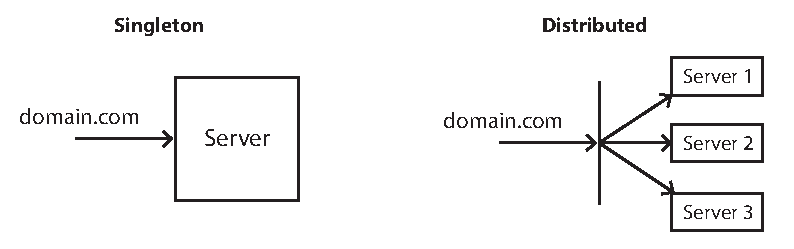
\includegraphics[width=\textwidth]{gfx/server_solutions.pdf}
    \caption{Illustration of a singleton and distributed server solution.}
    \label{fig:server_solutions}
\end{figure}

Distributed server solutions contain several servers possibly on several locations, meaning that DoS will be harder to perform, since there is no single point of failure.
However, this solution cannot ensure consistency and adds complexity.
The two solutions are graphically displayed in Figure~\ref{fig:server_solutions}.
A singleton solution has been chosen due to; consistency and simplicity.
This singleton solution will be denoted as Master or \deno{M}.

The application is required to handle communication with drones, as defined by \at{1} in Figure~\ref{tab:acceptance_tests1}.
In case of the communication being disabled, this might end up with a drone crash.
The technical limitations of antennas for digital wireless communication, sets a constraint for the availability of drones.
Assuming there exists no antenna to cover the physical area of our problem domain, it is necessary to have a distributed antenna setup in order to cover the whole physical area of the problem domain.
This leads to the structure shown in Figure~\ref{fig:antenna_structure}.

\begin{figure}[htb]
    \centering
    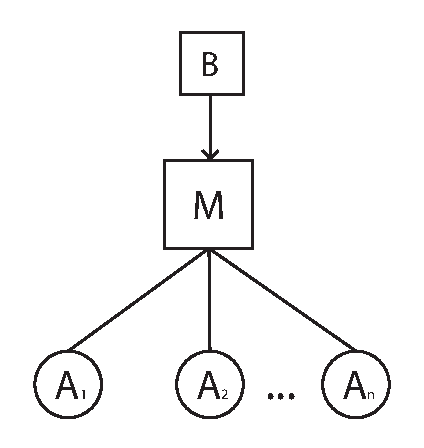
\includegraphics[width=0.5\textwidth]{gfx/antenna_structure.pdf}
    \caption{Antenna structure.}
    \label{fig:antenna_structure}
\end{figure}

If all \deno{B}'s communication with the drones goes through \deno{M}, this would create a single point of failure.
This means that, if \deno{M} crashes at any point, all communication with the drones will be disabled.
Providing the antennas with processing power and opportunity to communicate directly with \deno{B} would solve this issue.
If an antenna crashes only the drones connected to that antenna would be disconnected, leaving the drones connected to other antennas untouched.
This could be achieved by distributing some of the communication from \deno{M}.
This is solved by combining the antennas with distributed processing units, which will be denoted as Slaves or \deno{S}, as shown in Figure~\ref{fig:slave_structure}.

As \deno{S} has a dynamic network position relative to \deno{M}, this enforces that \deno{B} is not able to communicate directly with \deno{S} before getting network information about \deno{S} from \deno{M}. This communication is illustrated by a dashed line in Figure~\ref{fig:slave_structure}.

\begin{figure}[htb]
    \centering
    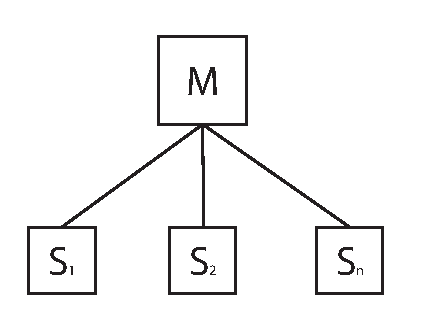
\includegraphics[width=0.5\textwidth]{gfx/slave_structure.pdf}
    \caption{Slave structure.}
    \label{fig:slave_structure}
\end{figure}

The acceptance tests, e.g. 17, 24, 25 in Figure~\ref{tab:acceptance_tests2}, enforces a constraint that requires \deno{M} to be able to store data based of the interaction of the user.
As requests can happen asynchronously, this makes it ideal to use a database denoted \deno{DB}, due to its transaction system in order to ensure no data loss.

The response output of \deno{M} needs to be dynamic based on the user, e.g. Acceptance test 2 in Figure~\ref{tab:acceptance_tests1}, which requires \deno{M} to be capable of processing data and store it in the database.
The processing unit that creates the dynamic response will be denoted \deno{W}.
The communication with the drones are handled by another processing unit, denoted \deno{D}.
If \deno{W} were to handle requests from \deno{S} and \deno{B}, this would increase the load on \deno{W}.
By creating multiple request handlers, it is possible to have a process for each. \deno{W}, \deno{DB}, and \deno{S} are processes, seen in Figure~\ref{fig:daemon_structure}, which improves resource management.
The resource management could be to constrain processing power for each process, or distribute the processes on individual machines.

\begin{figure}[htb]
    \centering
    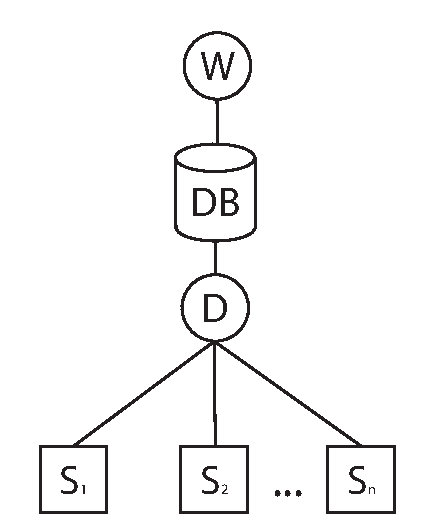
\includegraphics[width=0.5\textwidth]{gfx/daemon_structure.pdf}
    \caption{Daemon structure.}
    \label{fig:daemon_structure}
\end{figure}

% The architecture of \projectname{} differs from other web applications due to the fact that there exists two different type of servers.
% The architecture can be seen in figure~\ref{fig:system_architecture}.
% The server where the web application is running is called Master denoted M.
% For each drone in the system there is a Slave denoted S.
% On both M and S there exists daemons which is responsible for different tasks, however there is some similarity in the tasks they perform.
% These tasks can happen at anytime therefore the program needs to be running at anytime. These daemons are denoted D.
% Each user have a browser they view the application through this is denoted B.
% It is M's responsibility to communicate with every S in the system.
% S is responsible for all communication with the drone it is parred with.

% When a user wants to interact with a drone in the system a session key is needed.
% Such a session key is generated by S and then given to B through M.
% When both B and S have the same session key it is possible for them to communicate without M.
% This ensures that M does not become a bottleneck for controlling and streaming from drones and it reduces latency.
% When a new drone is added it is controlled by its S. This ensures that the system can scaled out and not have to scale up.
% Scale out means using more than one server where scale up means adding more processors, ram etc. to the server so it can handle more by itself.
% M does not handle commands and streaming, and every drone in the system have their own S.
% This makes the application architecture scalable because it removes bottlenecks from both M and S's.

% \begin{figure}[htb]
%     \centering
%     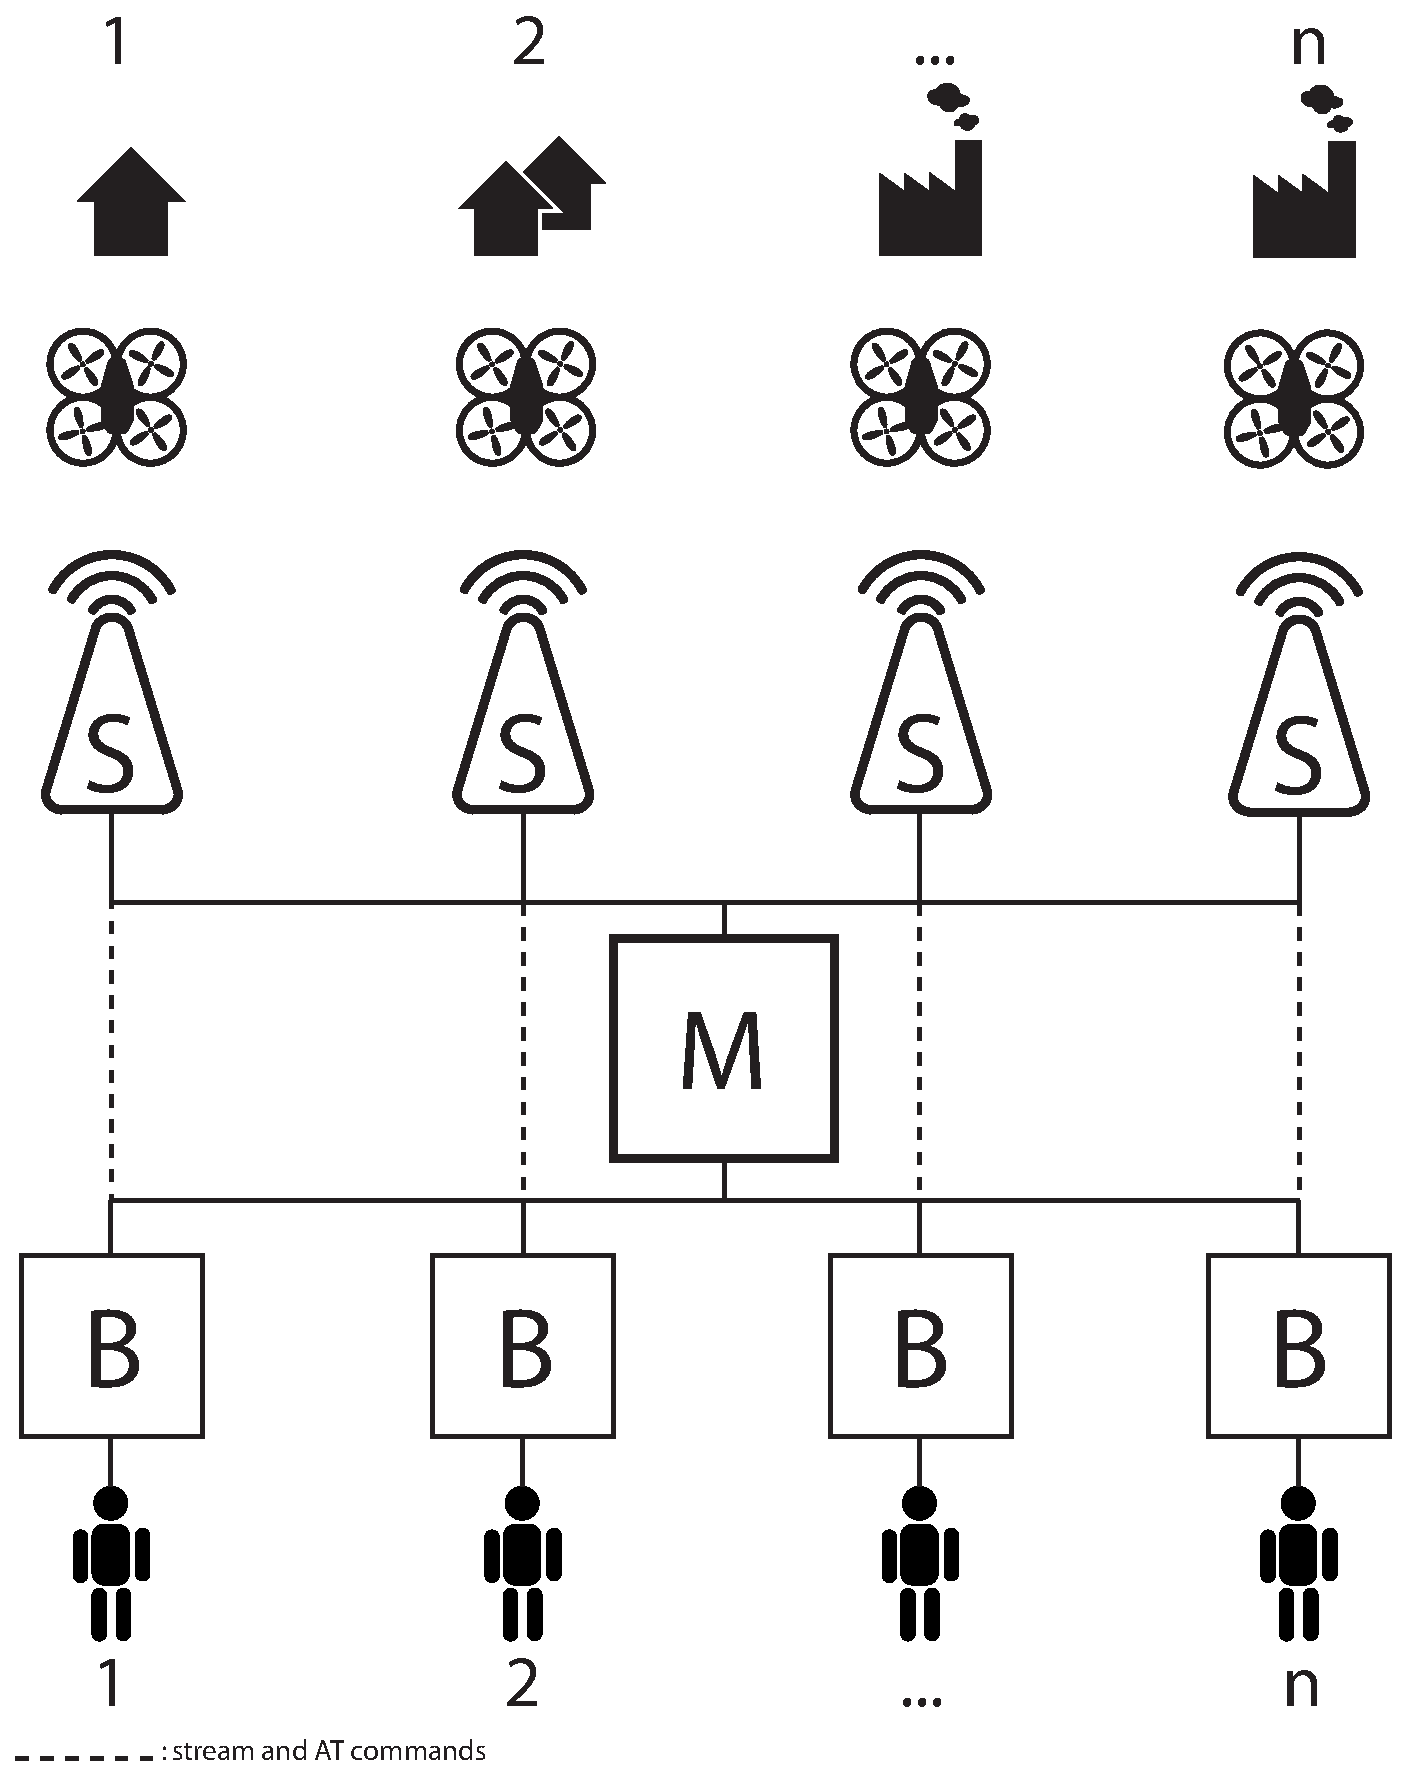
\includegraphics[width=\textwidth]{gfx/system_architecture.pdf}
%     \caption{System architecture of \projectname{}}
%     \label{fig:system_architecture}
% \end{figure}

% The system only uses one M. This can also be seen the bottleneck of the system.
% If M crashes all S's and B's will have to wait for M to come back up.
% One alternative could be running with more M's and in that way scale out.

% There is always one S for each drone connected to the system.
% In this way the system is scaled out.
% This ensures that any S is not likely to become a bottleneck.
% This was done because the drone uses wireless network which is short ranged and the drone is the host which means that the server needs one wireless connection for each drone it have to transmit to.
% One alternative could be only running with one S at each company and just scale it up.
% The problem with this is the server will need a wireless connection for each drone it have to control and it have to be in range.

% Daemon is a background process on a Linux system.
% Daemons are used when it is needed that a process is running at all times.
% In \projectname{} there are both the session key system which both resides on M and S and a policy file system for Adobe Flash on S.
% Both of these processes needs to be running at all times for the user to interact with the drone on S.
\section{Functionality distribution}\label{sec:functionality_distrubution}
% Hvilke funktionaliteter skal dækkes?
% Hvilke instancer dækker hvad?
% Hvorfor gør de det?

The functionality of the system can be derived from the acceptance tests.
This section will cover what instances are responsible for each functionality.

The need for storing data is derived from \at{1}, as previously described this is handled by the database \deno{DB}, which is a part of \deno{M}.
\at{2} sets the need for a dynamic response to \deno{B}, which requires processing of the stored data.
This processing is handled by Web or \deno{W} as the structure contains a singleton server solution.

Knowing that \deno{S} has a dynamic location relative to \deno{M}, this requires \deno{S} to send a signal to the daemon or \deno{D} in order for \deno{M} to get the location of \deno{S} on the network.
\deno{D} is then responsible for being able to receive incoming signals from \deno{S}.

Displaying video is required of \deno{B} by \at{3}.
The video displayed by \deno{B} is a stream, which requires that \deno{S} sends out a video stream.
In order to control a drone, commands have to be provided to the drone, as required by \at{3}.
\deno{S} is responsible for being able to receive commands and have the drone execute the given command.
\at{29} enforces security of the command handler.
\deno{S} is the only instance with a direct link to the drone, this makes \deno{S} responsible for the command handler's security.

% While Section~\ref{sec:application_structure} covered the overall structure of this application, this section will cover how the functionality is divided between the Master and the Slaves in the system. \\

% The Master is the users only way into the system.
% This access will always be via the users local web browser, where he sees the web system for \projectname{}.
% This web system and the database containing all informations about the system, drones, users etc. will be located on the Master.
% The Master is responsible for providing these services and coordinating the communication between the users and drones via the Slaves. \\

% A Slave is needed for every drone in the field, as the drones are not capable of long-distance communication.
% Therefore, in order to communicate with any drone, the communication must be channeled through its assigned Slave.
% This Slave is responsible for keeping contact with the drone and communicate directly with it via its API's.



\section{Communication network}\label{sec:communication_network}

Having functionality distributed across several instances sets the need for communication between the instances.
Based on Figure~\ref{fig:slave_structure}, which displays the dependency between \deno{B}, \deno{M}, and \deno{S} this leads to the diagram shown in Figure~\ref{fig:dataflow_diagrem}. \\


\begin{figure}[!h]
    \centering 
    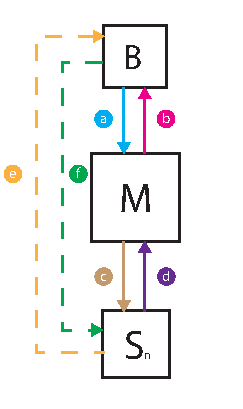
\includegraphics[width=0.5\textwidth]{gfx/dataflow_diagram.pdf}
    \caption{Dataflow diagram of \projectname{}}
    \label{fig:dataflow_diagrem}
\end{figure}


The arrows represent a connection, each connection represent dataflow in the direction of the arrow.
The type of data flowing in each connection and the reasons behind will be covered as each connection is discussed below. \\

Connection \deno{a} covers requests made by \deno{B}, which covers HTTP requests, which is a limit of web solutions that they must use the HTTP protocol.
HTTP requests enable the user to view the web application through his browser, and to send information.
In order to fulfill the request created by \deno{a}, a response is needed which the connection \deno{b} handles.
This connection covers the flow of the dynamic content created by \deno{M}, and static content such as: images, stylesheets, and multimedia objects.
Connection \deno{b} sends both the static and dynamic content back to \deno{B} to be displayed for the user. \\

The connection \deno{d} handles the signal described in Section~\ref{sec:functionality_distribution}.
This signal covers the initial communication between \deno{S} and \deno{M}. \deno{M} verifies the identity of \deno{S} by \deno{S} sending its own unique identifier.
This unique identifier is a string, which consist of X characters \fixme{How many chars?}.
All unique identifiers of each \deno{S} is known to \deno{M}.
This allows \deno{M} to determine the identity of each incoming signal. When \deno{M} receives a signal, and verify the identity of \deno{S}, the source location of the signal is stored in \deno{M} making \deno{M} able to know the location of \deno{S}. \\

Since requests from \deno{B} can happen asynchronously and from dynamic locations, it can create a problem that the identity of the connection made from \deno{S} to \deno{f} is not known. 
\at{28} sets the requirement of differentiating between incoming connections to \deno{S}.
If the communication described in connection \deno{e} and connection \deno{f} were running through \deno{M}, this would be no problem as security would be handled by the already existing sessions on \deno{M}.
The connections \deno{e} and \deno{f} are required to transport a large amount of data.
This data covers a video feed of the drone's video camera and commands for the drone.
This would increase the load on \deno{M}, which is not desired as \deno{M} is assumed to have a high load already.
However, since connection \deno{e} and connection \deno{f} are not running through \deno{M}, this leaves the problem of which \deno{B}, \deno{S} should listen to. \\

The solution chosen to solve this problem is to make \deno{S} create a randomly generated key (session key), that contains 40 characters and is unique relative to \deno{S} stored on \deno{S} itself.
When \deno{S} receives incoming commands, \deno{S} verifies whether or not the key received along with the command is equal to the one locally stored on \deno{S}.
If this is the case, \deno{S} classifies the received command as valid and performs the action.
The session key is delivered to \deno{B} from \deno{M}, as \deno{M} is able to verify the identity of \deno{B} through the session. \\

The connection \deno{c} covers requesting a session key by \deno{M}.
As \deno{M} has a static location, \deno{S} is able to verify the identity of \deno{M} based on its location.
Connection \deno{d} covers the response of the request received in \deno{c}, and \deno{M} is able to verify the identity of \deno{S} based on its location. \\

\begin{figure}[!h]
    \centering 
    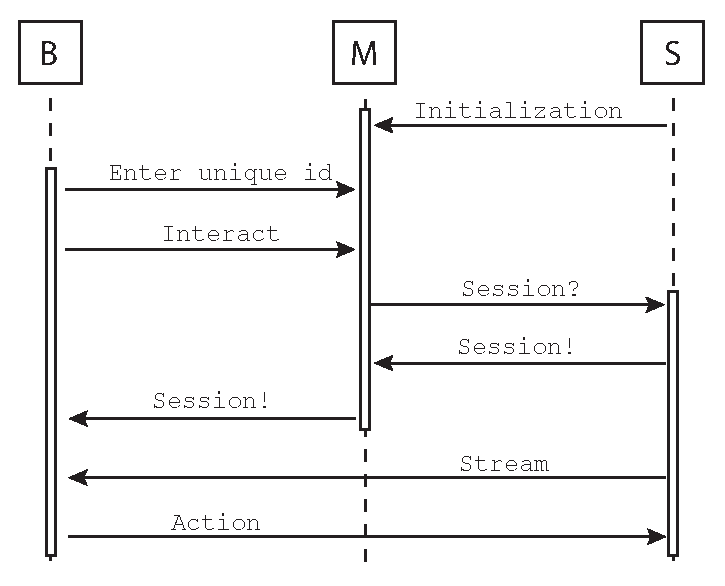
\includegraphics[width=\textwidth]{gfx/sequence_diagram.pdf}
    \caption{Sequence diagram of the communication network between \deno{B}, \deno{M}, and \deno{S}}
    \label{fig:sequence_diagram}
\end{figure}
\fxfatal{Check UML notation.}


The functionalities of the described connections, can only happen in a sequence as illustrated in Figure~\ref{fig:sequence_diagram}.
Each message in the sequence diagram can be done multiple times, however above messages are enforced to be performed atleast once in order for the given message to be performed. \\


% The communication network is crucial for \projectname{} to work.
% When designing a scalable communication network it is important to choose the right structure.
% There are different ways when designing such a network but identical for them all is that they need to support the structure of \deno{M}, \deno{S} and \deno{B} described in section~\ref{sec:application_structure}.

% One solution is to make a structure where \deno{M}, \deno{S} and \deno{B} talk to each other with a level of security. 
% The security aspect would be implemented with a form of session key. 
% This key would be used to determine if a session between a \deno{B} and a \deno{S} is valid.
% Another solution is to provide no security aspect and let it be up to the users and / or company to keep drones safe from intruders.
% This would lessen the communication between \deno{B}, \deno{M} and \deno{S}.  
% It would also decrease the load on \deno{M} and \deno{S}'s database. 
% On the down side the system could be considered not safe because it would be possible to tamper with the drones.
% As this is a system where it is important that the integrity is high, evidence is not tampered with, and where the outcome of an unauthorized user controller a drone could be devastating, it is important to deliver some form of security.



% This lead to a solution where sessions is designed to keep the integrity and secure evidence as seen in figure~\ref{fig:sequence_diagram}. 
% As seen in the figure there is designed a level of security because of the sessions.
% It is not possible for a \deno{B} to interact with a drone without having a session with a drones \deno{S}.

% When a drone is purchased a \deno{S} is setup at the location where the drone is going to operate.
% The \deno{S} sends an initializing message to \deno{M}, informing \deno{M} that a new drone has entered the system.
% \deno{M} adds the drone with the IP and location of the \deno{S}, along with the drone's unique identifier.
% If \deno{M} receives an initializing message from a \deno{S} with a drone identifier that is already in the system, it will destroy any session that correlates with that drone.
% The sessions is destroyed because if one or more sessions are granted and \deno{S} sends its initializing message it is safe to assume that \deno{S} either disconnected or crashed and all sessions keys are invalid.
% Furthermore if the IP of \deno{S} differs from the IP \deno{M} holds in its database it will be updated.

% If a user tries to interact with a drone the system behaves differently.
% A session key will be made on a \deno{S}, this key will be send to \deno{M} and giving to \deno{B}. If this session key is valid it is possible for the user to communicate directly with \deno{S} without \deno{M}.

% \begin{figure}[!h]
%     \centering 
%     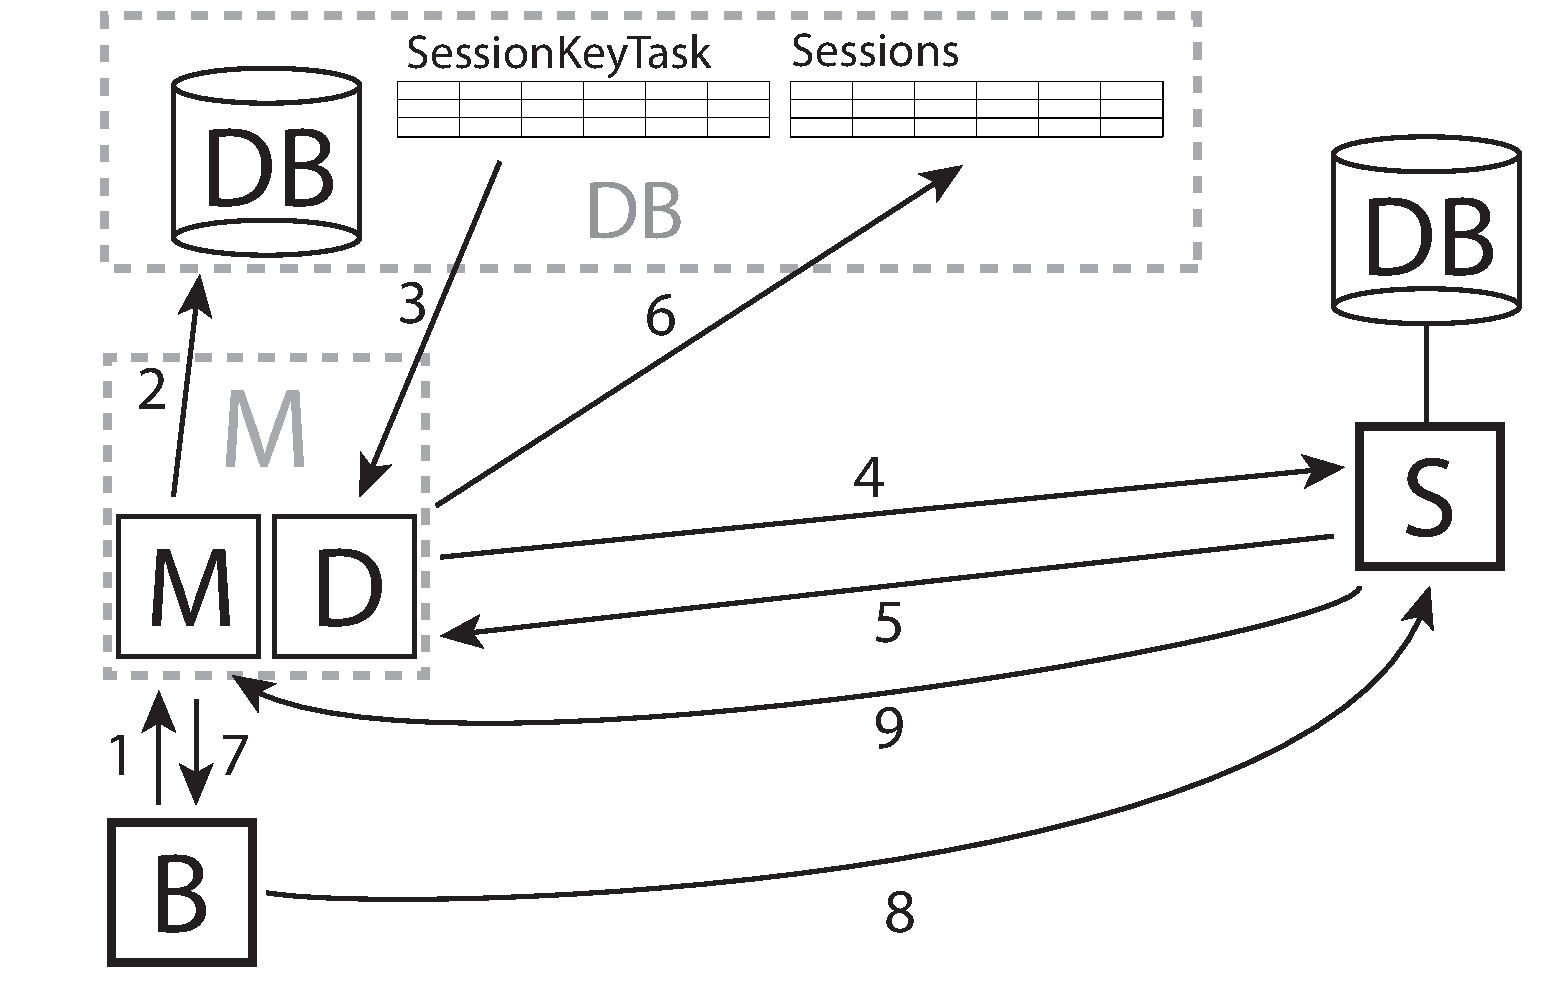
\includegraphics[width=\textwidth]{gfx/sessionkey_communication.pdf}
%     \caption{Session key communication between \deno{B}, \deno{M}, and \deno{S}}
%     \label{fig:sessionkey_communication}
% \end{figure}

% This behavior can be seen in figure~\ref{fig:sessionkey_communication}. 

% Session keys have been designed for security reasons.
% Firstly they were designed to ensure that only one user at a time can control a drone.
% Secondly it ensured that unauthorized users do not have the possibility of controlling a drone.

% \begin{enumerate}
% 	\item Request send from \deno{B} to \deno{M} about getting a session key to interact with a drone.
% 	\item \deno{M} inserts this request in its database table called SessionKeyTask.
% 	\item \deno{D} scans the database table SessionKeyTask, when it sees a new entry it select it and then deletes it from the table.
% 	\item \deno{D} requests a session key from \deno{S} parred with the drone the user wants to interact with.
% 	\item \deno{S} makes a random generated string with uppercase, lowercase letters and number. This string is used as the session key. \deno{S} updates its database with this session key and then sends it back to \deno{D} on \deno{M}.
% 	\item \deno{D} inserts the newly received session key into the session table of \deno{M}.
% 	\item \deno{M} then contacts \deno{B} with the session key.
% 	\item \deno{B} uses this session key to access \deno{S} and through it interact with the drone.
% 	\item A Timeout happens if \deno{B} and \deno{S} does not communicate for 10 seconds.
% \end{enumerate}

% Communication between the servers in the system is crucial. 
% Therefore it is important design a method or a set of methods handling the communication between them. 
% One method could be to make a service which handles all these requests on each server.
% The problem however is that using a single service might create a bottleneck.
% An alternative solution is to make a service for each communication level.
% One service that handles sessions, a service that handles control commands, and a service that handles initial messages from \deno{S} see section~\ref{sec:application_structure}.\fxfatal{Den her paragraf er uspecifik}

% This lead to a solution where the different actors in the system delivered and / or depended on services.

% The interface of the communication network can be seen in figure~\ref{fig:communication_network}.

% The communication network of \projectname{} uses four different ports for providing its services:

% \begin{itemize}
% 	\item Port A - service port for sending and receiving drone control commands.
% 	\item Port B - service port for receiving and sending initial messages.
% 	\item Port C - service port for sending and receiving session information including session keys.
% 	\item Port Web - service port for sending and receiving web specific information.
% \end{itemize}

% \begin{figure}[!h]
%     \centering 
%     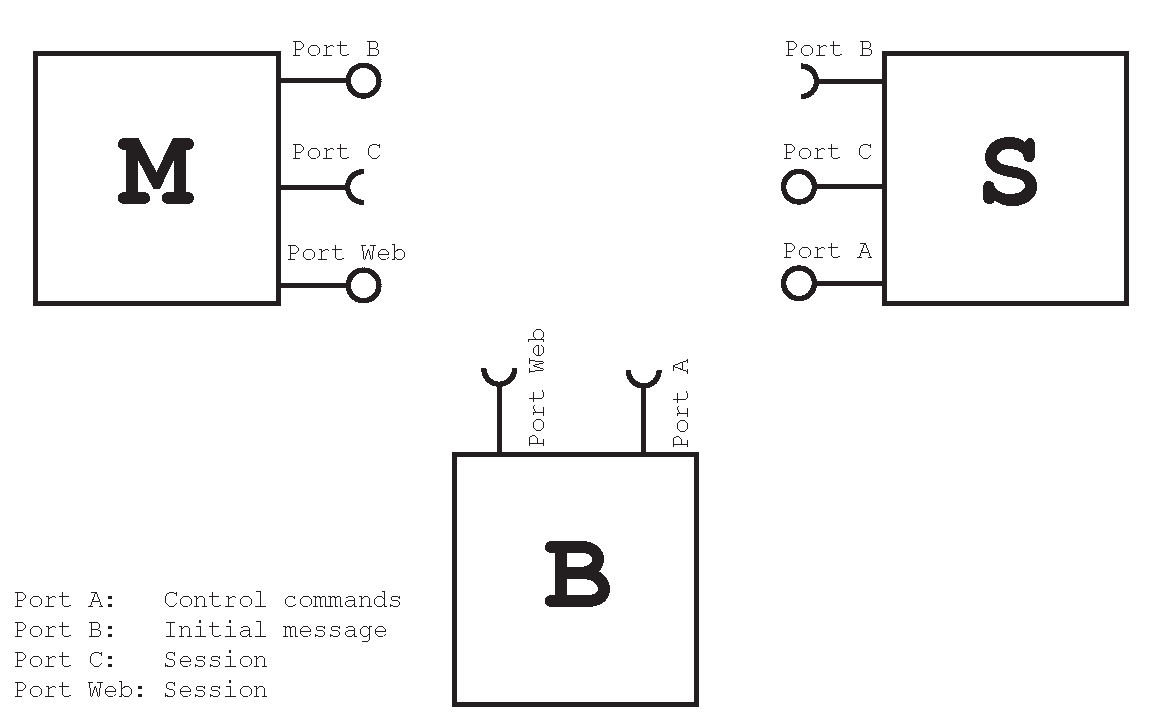
\includegraphics[width=\textwidth]{gfx/communication_network.pdf}
%     \caption{Communication network between \deno{B}, \deno{M}, and \deno{S}}
%     \label{fig:communication_network}
% \end{figure}

% When designing a communication network it is also important to select the right technique for exchanging data between services.
% One of the more widely used techniques are Extensible Markup Language.
% Extensible Markup Language, or XML for short, is a markup language designed to easily mark up data.
% The markup that XML provides makes it possible to easily send and receive data.
% The Extensible in XML makes it possible to extent what data types XML can handle through the XML schema. \citep{simonstl}
% This gives XML a drawback because XML is designed to be extensible it also carries a lot of overhead when used to mark up data.

% \projectname{} needs to be scalable therefore it is important to use as little overhead when sending structured information.
% Otherwise there is a chance that this overhead creates a bottleneck within the network.

% JSON, or JavaScript Object Notation, is design for data interchange and to be human-readable.
% It have a simpler syntax than XML and is not build to be extensible, it is not even a markup language. 
% It is a structured way of exchanging data between sources. 
% This results in less overhead i.e. it costs less data for each piece of information. 
% JSON is also data orientated which makes it easier to map a JSON object directly to a object orientated structure.
% Douglas Crockford call JSON ``The Fat-Free Alternative to XML'' \citep{JSON}.

% Therefore JSON is the perfect format for data interchange between the different services in \projectname{}. There are lesser costs associated with JSON than XML and it is easier to map them into a object orientated language.
\section{Object Model}
\label{section:uml_notation}
\label{subsec:objects}

This section will cover the design choices behind the application's object model, derived from the use cases in Section~\ref{sec:use_cases}.
The UML object model diagram can be seen in Figure~\ref{fig:UML_class_diagram}, and is guided by the UML standard guide written in cooperation by several different software companies~\citep{UML_notation}.\\

The UML attribute notation in this report is:
\begin{itemize}
    \item PK attribute - means that the attribute is a primary key.
    \item FK attribute - means that the attribute is a foreign key.
    \item attribute : type - all attributes will have a type e.g. \verb+id : int+.
\end{itemize}

The system will contain the following objects: \deno{Affiliate Privilege}, \deno{Company}, \deno{Drone}, \deno{Privilege}, \deno{Role}, \deno{Session}, and \deno{User}.
The model of the objects and their relationships can be seen in Figure~\ref{fig:UML_class_diagram}.
Each object covered is represented in the object model diagram with its name in lowercase and pluralized, e.g. \deno{User} object $\rightarrow$ \deno{users}.
If an object's name consists of several words the spaces will be replaced by underscores, e.g. Session Key Task becomes session\_key\_tasks.
The relationships between objects can either be implicit with a line directly from one object to another, or explicit with a simple or rich relationship model between the two objects.
Simple relationship models are models without a PK.
They are represented in the model diagram with both objects in lowercase and pluralized, e.g. roles\_users.
Rich relationship models have a PK.
This kind of relationship model does not have a predetermined naming convention, therefore it can be anything as long as it does not collide with the other model names, e.g. user\_privileges.\\

\begin{figure}[htb]
    \centering
    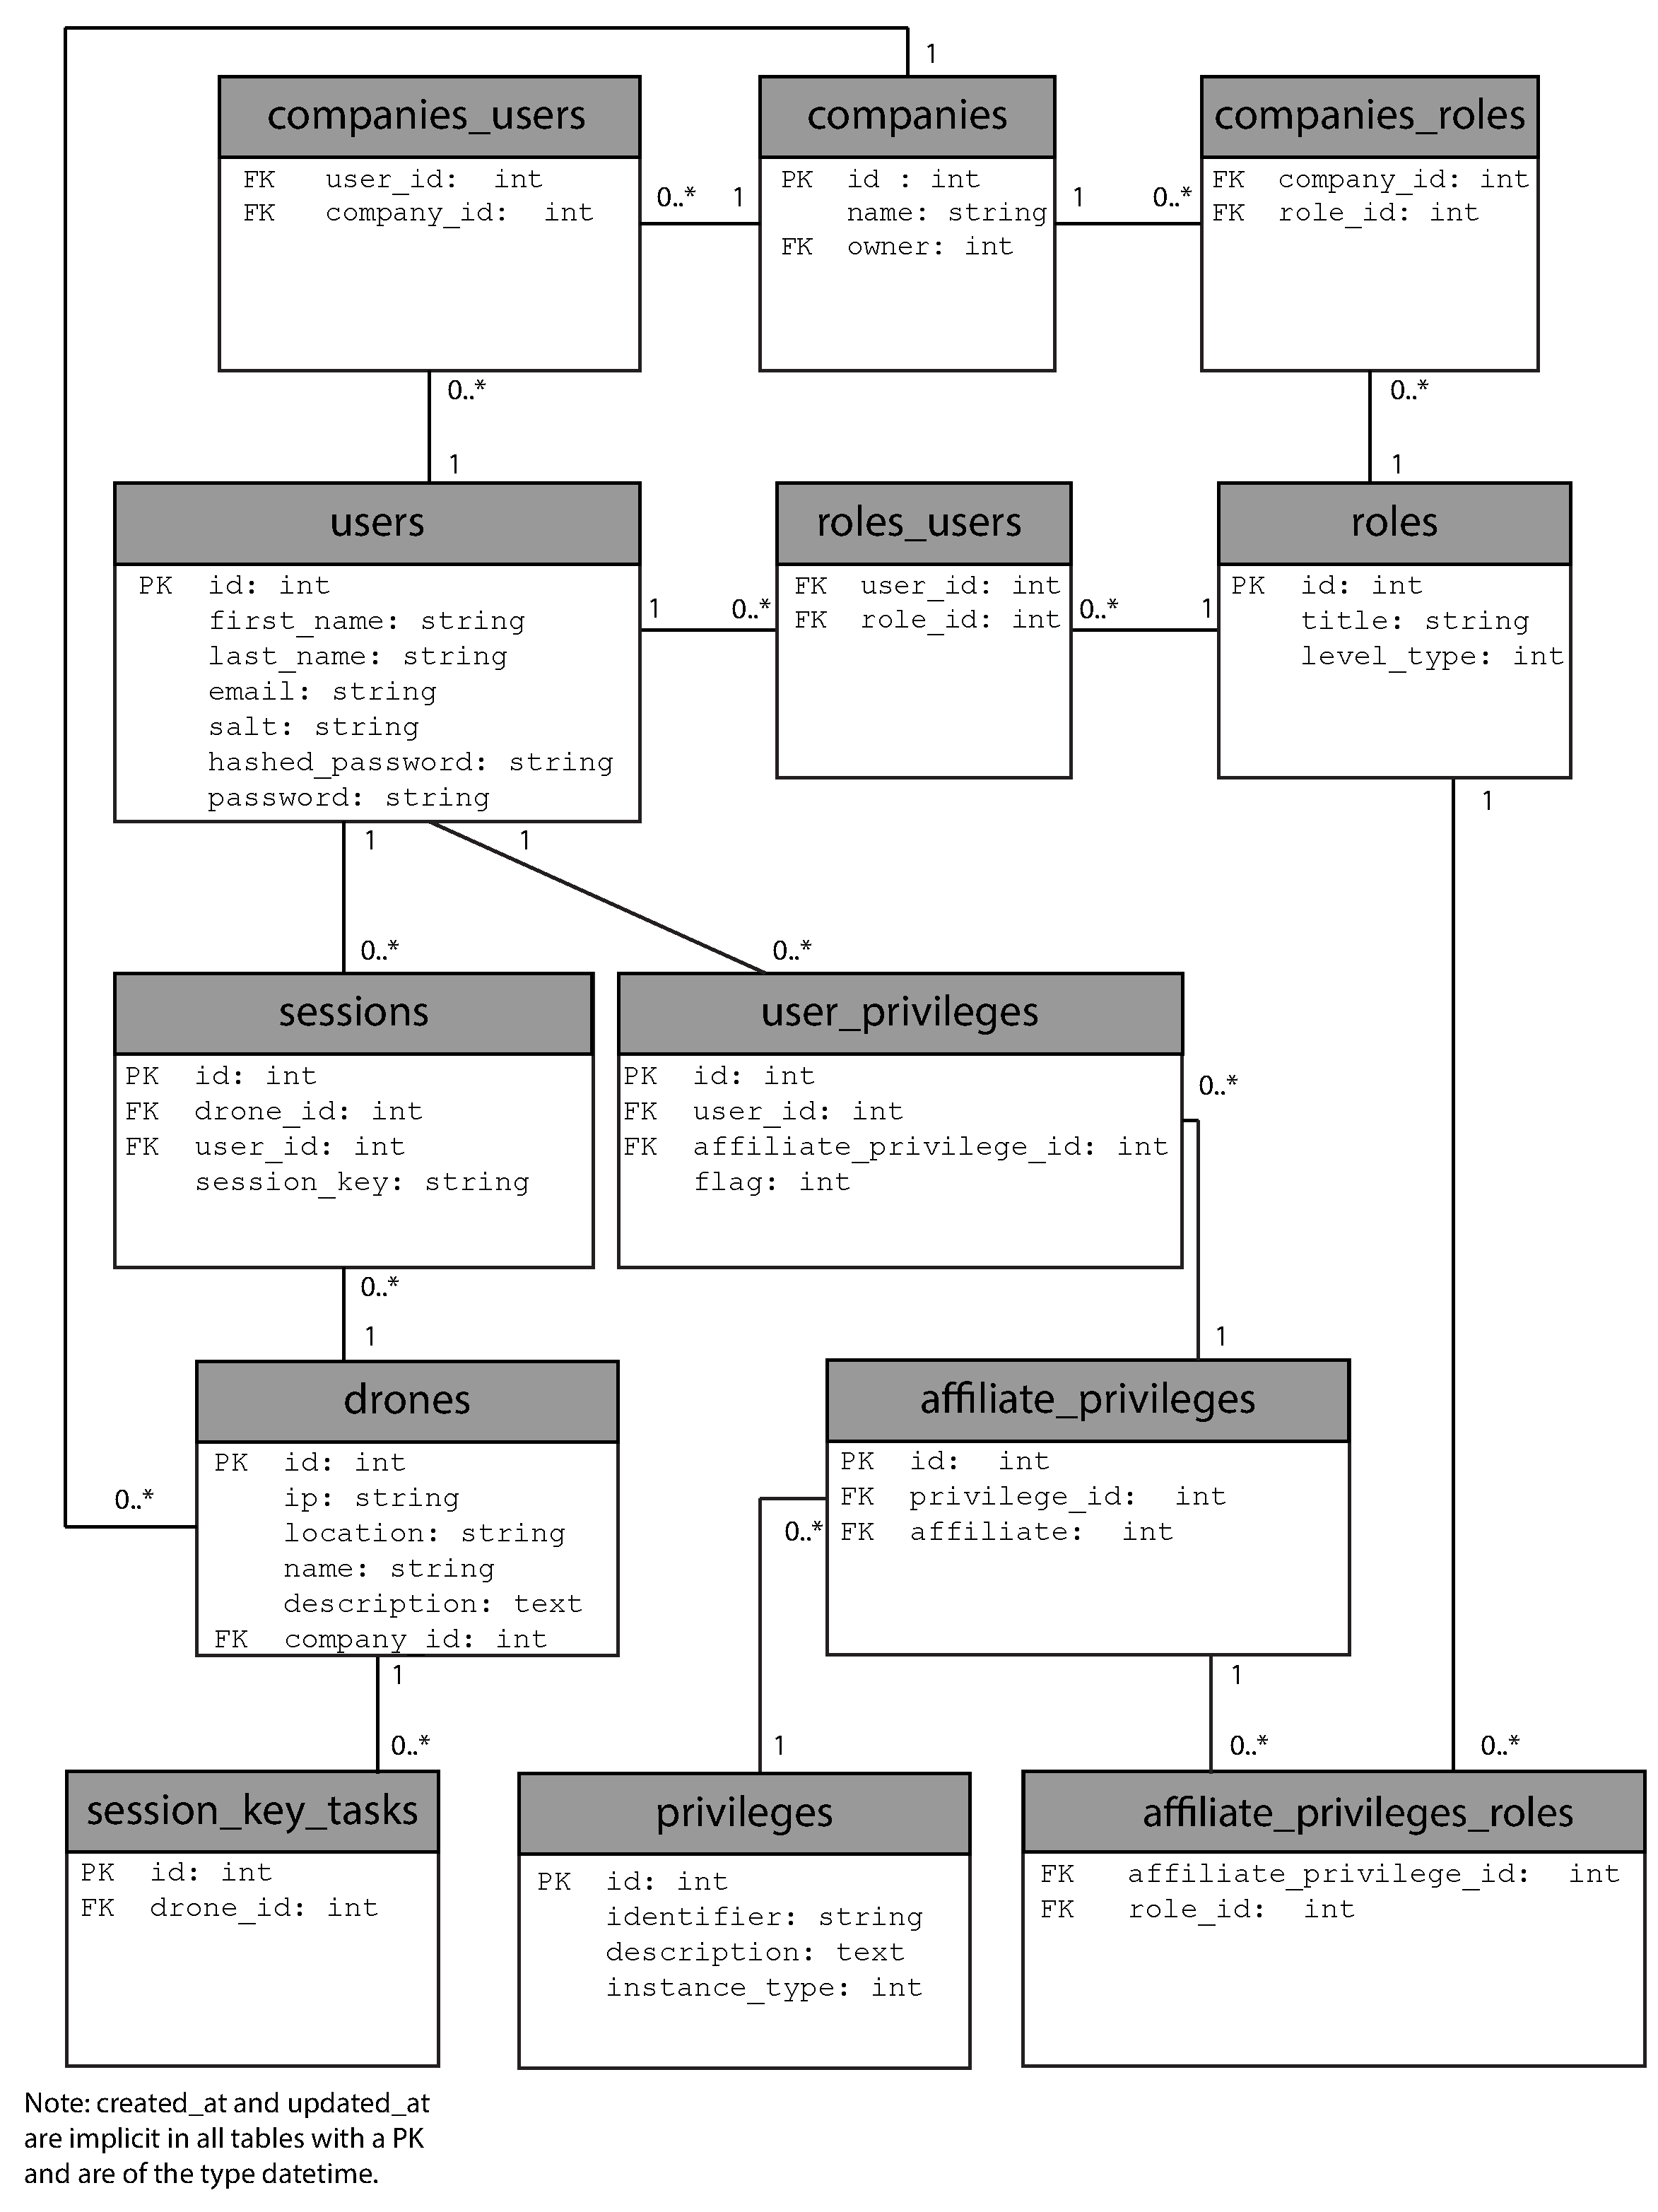
\includegraphics[width=0.95\textwidth]{gfx/UML_model.pdf}
    \caption{UML Class Diagram of \projectname{}}
    \label{fig:UML_class_diagram}
\end{figure}


\subsection{Objects}\fixme{Skal denne overskrift være der? Det burde ikke være nødvendigt at have den, men så skal teksten ændres lidt.}
Access to and actions of the system is restricted.
This restriction is based on the identity of user in the system.
An instance of the \deno{User} object represents a user to the system.
The \deno{User} object has the attributes \verb+email+ and \verb+password+, as seen in Figure~\ref{tab:user_object} in Appendix~\ref{app:objects}, these combined form the login credentials needed for a user to authenticate his identity towards the system. \\

The \verb+email+ is publicly available, which leaves the \verb+password+ to be protected in order for user to protect his identity in the system.
The \verb+password+ entered by the user is concatenated with a \verb+salt+ and hashed through a SHA-1 hashing algorithm to be stored in \verb+hashed_password+.
The hashing algorithm provides a way for storing the password without having its exact value, as this could leave to a security flaw.
Having access to passwords of users directly, e.g. through a hacker attack, would allow the hacker to login into the users account, which is unintended for the system.
When a salt is concatenated before hashing it makes it harder for the hacker to gain the original passwords, e.g. through a rainbow table~\cite{something}. \\

Having a distributed setup with multiple \deno{S}, each representing a \deno{Drone} object, means that the network locations of these need to be known in order to communicate.
The network location is stored in the \verb+ip+ field of the \deno{Drone} object, as shown in Figure~\ref{tab:drone_object} of Appendix~\ref{app:objects}.
The physical drone have a unique identifier known as \verb+name+, which makes the user able to identify a given drone. \\

The users of the system will be part of different companies, therefore there is a need for grouping users by a company.
The \deno{Company} object have an \verb+owner+, which is a reference to a \deno{User} object.
This is required for the system to know which user have access to all \deno{Affiliate Privilege} objects of the company. \\

An \deno{Affiliate Privilege} object references a \deno{Privilege}, and only when combined they form a unique key.
This key unlocks a certain functionality, meaning that if the user does not have a relation to the \deno{Affiliate Privilege} object, which represents the key, then the user is not able to unlock that functionality.
\deno{Role} objects give the possibility of grouping \deno{Privilege} objects together.
Each \deno{Company} have a related role which contains all privileges, of which the company have full control.
Full control gives the right for passing on a privilege, or disabling if the privilege is already granted.
\deno{Affiliate Privilege} objects have a field \verb+affiliate+ that links the privilege to an object of the type declared by the referenced \deno{Privilege} object's \verb+instance_type+ field. \\

The \deno{Session} object represents an active pilot connection between a user and a drone.
The \verb+session_key+ field provides a key that needs to be sent along with the commands.
The \deno{Session Key Task} object is an object used for \deno{D} and \deno{M} to communicate through \deno{DB}, as shown in Figure~\ref{fig:daemon_structure} in Section~\ref{sec:application_structure}. \\

In Section~\ref{sec:privileges} solutions for handling privileges were discussed.
From this discussion it was decided to model a system capable of handling all proposed solutions to fit scenarios of the users.
The \deno{User Privileges} relationship allows for connecting individual {Privilege} objects to a \deno{User} object.
This is could be either granting or revoking, i.e. exceptions, the privilege.
The \verb+flag+ field represents a value of either 1 or -1; 1 is regarded as granted, and -1 is regarded as revoked.


% \subsection{Relationships}
% The system is designed with flexibility and scalability in mind, and the structure of Roles and Privileges are what provides those features.
% As described before there are two ways that a User can be granted a specific Privilege.
% These are by 1) getting the Privilege granted directly via the \verb+User_Privileges+ table or 2) by being a member of a Role that via the \verb+Privileges_Roles+ table that has one or more Privileges granted.
% These will be explained in details in the following subsections.


% % Users and Privileges %
% An administrator can grant a specific Privilege directly to a user via the \verb+User_Privileges+ table.
% This Privilege is then affiliated with an object -- usually a Drone.
% The Privilege could also be a system functionality, however, as described in Section~\ref{sec:privileges}. \\

% This relationship is also used for exceptions.
% In an example where five Users: U1, U2, U3, U4 and U5 are a member of a Role: R1, we may have a situation where U2 is not suppose to have access to a given Privilege P1 in R1.
% Then a User-specific Privilege is granted to U2 on P1, but with the ``exception''-flag marked.
% This is equal to blacklisting U2 from using Privilege P1, providing the system with a lot of flexibility, as even though a group of Users are granted a number of Privileges via a role, User-specific exceptions can be added to this setting. \\


% % Roles and Privileges %
% As mentioned before -- the reason that Roles can be used to assign Privileges to a User, is to make both the administration and data structure of Users and Privileges as simple and efficient as possible.
% By allowing exceptions, full flexibility is still possible. \\

% This is how the relationship between Roles and Privileges works: \\

% An administrator creates a Role.
% Lets call this Role ``Control Drone \#4''.
% A number of Privileges are assigned to this Role.
% It could be the following:

% \begin{itemize}
%     \item Watch the video feed from a specific drone
%     \item Control the movement of a specific drone
% \end{itemize}

% Those Privileges are then linked to this Role and to the Drone this concerns. \\

% Roles can be assigned with affiliation to both Users and Companies.
% Say a user \verb+U1+ needs access to Drone \#4.
% User U1 then needs to either have the Privileges directly granted or be a member of the role ``Control Drone \#4''.


% % Privileges and granting of Privileges %
% Since it is possible to grant Privileges both directly to a User and via a Role, the same Privilege can be used in more than one context.
% Therefore the \verb+Affiliation_Privileges+ table exists.
% This table links the granting of a Privilege with the actual Privilege and defines on which Object the Privilege applies.
% The reason for having this table and not just link the two granting-tables \verb+User_Privileges+ and \verb+Privileges_Roles+ directly to the \verb+Privileges+ table, is that we try to avoid redundant data by having the data in the \verb+Privileges+ and \verb+Affiliation_Privileges+ table make up one instance of a privilege together.
% This is then granted to a User or a Role, who can then use the Privilege. \\

% The system is designed so that any User can grant a Privilege he already has already been granted to another User if he is permitted to.
% This is controlled via a ``re-grantable'' flag which is set in either the \verb+User_Privileges+ table or the \verb+Privileges_Roles+ table.
% By marking this flag as ``true'', the User or Users that via a Role is granted the Privilege in question, can via an interface in the system re-grant the Privilege to other Users in the same Company.


% %Note: Alle brugere kan videregrante et privilege hvis de har tilladelse til det. Det er et flag som sætes i user_privileges og privileges_roles, som tillader alle der har dette privilegie til at videregrante det. Husk at beskrive hvordan et privilege og et affiliation privilege til sammen giver et grant-able privilegie


% % Privileges and Drones %
% With \projectname{} in its current form, most Privileges that are granted will have an connected with a Drone.
% Privileges and its a affiliations are linked in the \verb+Affiliation_Privileges+ table.
% This is also where Drones are linked to any granted privilege. \\

% As described earlier, Drones are the current object-type implemented in the system.
% However, the structure and model of the system allows for later expansion, connection new objects such as stationary cameras or any other type of object to the system.
% The \verb+Affiliation_Privileges+ has a third field named \verb+object_id+.
% This field links the Privilege, the granting of it and the Object that this granting is valid for. \\

% An example could be linking Privilege P1, User U1 and Drone D1.
% Say P1 is the privilege for watching the video feed of a drone.
% Then the user U1 will have access to watch the video feed of Drone D1.


% % Drones and Companies %
% The \verb+Company_drones+ table defines a relationship between a Drone and a Company.

% The administrator of each Company defines the Roles in that Company.
% In doing so, he defines which Privileges that are granted in every Role.
% These Privileges are linked to a (Drone)-object.
% The system must make sure that any Company administrator cannot link a Privilege with a Object that is not within his control. \\

% This relationship defines which Drones are available to each Company.
% When a Company administrator adds new Roles (and hence Privileges), he is only able to associate it with Drones that are connected to the Company in question.

% **************************************************************************************************************
% A Classic Thesis Style
% An Homage to The Elements of Typographic Style
%
% Copyright (C) 2012 Andr\'e Miede http://www.miede.de
%
% If you like the style then I would appreciate a postcard. My address
% can be found in the file ClassicThesis.pdf. A collection of the
% postcards I received so far is available online at
% http://postcards.miede.de
%
% License:
% This program is free software; you can redistribute it and/or modify
% it under the terms of the GNU General Public License as published by
% the Free Software Foundation; either version 2 of the License, or
% (at your option) any later version.
%
% This program is distributed in the hope that it will be useful,
% but WITHOUT ANY WARRANTY; without even the implied warranty of
% MERCHANTABILITY or FITNESS FOR A PARTICULAR PURPOSE.  See the
% GNU General Public License for more details.
%
% You should have received a copy of the GNU General Public License
% along with this program; see the file COPYING.  If not, write to
% the Free Software Foundation, Inc., 59 Temple Place - Suite 330,
% Boston, MA 02111-1307, USA.
%
% **************************************************************************************************************
% Note:
%    * You must not use "u etc. in strings/commands that will be spaced out (use \"u or real umlauts instead)
%    * New enumeration (small caps): \begin{aenumerate} \end{aenumerate}
%    * For margin notes: \marginpar or \graffito{}
%    * Do not use bold fonts in this style, it is designed around them
%    * Use tables as in the examples
%    * See classicthesis-preamble.sty for useful commands
% **************************************************************************************************************
% To Do:
%		 * [high] Check this out: http://www.golatex.de/koma-script-warnung-in-verbindung-mit-listings-package-t2058.html
%    * [medium] mathbb in section-titles/chapter-titles => disappears somehow in headlines!!!
% **************************************************************************************************************
\documentclass[ twoside,openright,titlepage,numbers=noenddot,headinclude,%1headlines,% letterpaper a4paper
                footinclude=true,cleardoublepage=empty,abstractoff, % <--- obsolete, remove (todo)
                BCOR=5mm,paper=a4,fontsize=11pt,%11pt,a4paper,%
                ngerman,american,%
                ]{scrreprt}

%********************************************************************
% Note: Make all your adjustments in here
%*******************************************************
% ****************************************************************************************************
% classicthesis-config.tex
% formerly known as loadpackages.sty, classicthesis-ldpkg.sty, and classicthesis-preamble.sty
% Use it at the beginning of your ClassicThesis.tex, or as a LaTeX Preamble
% in your ClassicThesis.{tex,lyx} with \input{classicthesis-config}
% ****************************************************************************************************
% If you like the classicthesis, then I would appreciate a postcard.
% My address can be found in the file ClassicThesis.pdf. A collection
% of the postcards I received so far is available online at
% http://postcards.miede.de
% ****************************************************************************************************

% ****************************************************************************************************
% 1. Configure classicthesis for your needs here, e.g., remove "drafting" below
% in order to deactivate the time-stamp on the pages
% ****************************************************************************************************
\PassOptionsToPackage{eulerchapternumbers,listings,drafting,%
				 pdfspacing,%floatperchapter,%linedheaders,%
				 subfig,beramono,eulermath,parts}{classicthesis}
% ********************************************************************
% Available options for classicthesis.sty
% (see ClassicThesis.pdf for more information):
% drafting
% parts nochapters linedheaders
% eulerchapternumbers beramono eulermath pdfspacing minionprospacing
% tocaligned dottedtoc manychapters
% listings floatperchapter subfig
% ********************************************************************

% ********************************************************************
% Triggers for this config
% ********************************************************************
\usepackage{ifthen}
\newboolean{enable-backrefs} % enable backrefs in the bibliography
\setboolean{enable-backrefs}{false} % true false
% ****************************************************************************************************


% ****************************************************************************************************
% 2. Personal data and user ad-hoc commands
% ****************************************************************************************************
\newcommand{\myTitle}{LONE\xspace}
\newcommand{\mySubtitle}{Lone is Observation of Nondeterministic Environments\xspace}
%\newcommand{\myDegree}{Doktor-Ingenieur (Dr.-Ing.)\xspace}
\newcommand{\myName}{SW701E12\xspace}
\newcommand{\myProf}{Put name here\xspace}
\newcommand{\myOtherProf}{Put name here\xspace}
\newcommand{\mySupervisor}{Put name here\xspace}
\newcommand{\myFaculty}{Put data here\xspace}
\newcommand{\myDepartment}{Put data here\xspace}
\newcommand{\myUni}{Aalborg University\xspace}
\newcommand{\myLocation}{Aalborg\xspace}
\newcommand{\myTime}{December 2012\xspace}
\newcommand{\myVersion}{version 4.1\xspace}
\newcommand{\projectname}{<projectname>}

% ********************************************************************
% Setup, finetuning, and useful commands
% ********************************************************************
\newcounter{dummy} % necessary for correct hyperlinks (to index, bib, etc.)
\newlength{\abcd} % for ab..z string length calculation
\providecommand{\mLyX}{L\kern-.1667em\lower.25em\hbox{Y}\kern-.125emX\@}
\newcommand{\ie}{i.\,e.}
\newcommand{\Ie}{I.\,e.}
\newcommand{\eg}{e.\,g.}
\newcommand{\Eg}{E.\,g.}
% ****************************************************************************************************


% ****************************************************************************************************
% 3. Loading some handy packages
% ****************************************************************************************************
% ********************************************************************
% Packages with options that might require adjustments
% ********************************************************************
\PassOptionsToPackage{latin9}{inputenc}	% latin9 (ISO-8859-9) = latin1+"Euro sign"
 \usepackage{inputenc}

%\PassOptionsToPackage{ngerman,american}{babel}   % change this to your language(s)
% Spanish languages need extra options in order to work with this template
%\PassOptionsToPackage{spanish,es-lcroman}{babel}
 \usepackage{babel}

\PassOptionsToPackage{square,numbers}{natbib}
 \usepackage{natbib}

\PassOptionsToPackage{fleqn}{amsmath}		% math environments and more by the AMS
 \usepackage{amsmath}

% ********************************************************************
% General useful packages
% ********************************************************************
\PassOptionsToPackage{T1}{fontenc} % T2A for cyrillics
	\usepackage{fontenc}
\usepackage{textcomp} % fix warning with missing font shapes
\usepackage{scrhack} % fix warnings when using KOMA with listings package
\usepackage{xspace} % to get the spacing after macros right
\usepackage{mparhack} % get marginpar right
\usepackage{fixltx2e} % fixes some LaTeX stuff
\PassOptionsToPackage{printonlyused,smaller}{acronym}
	\usepackage{acronym} % nice macros for handling all acronyms in the thesis
%\renewcommand*{\acsfont}[1]{\textssc{#1}} % for MinionPro
\renewcommand{\bflabel}[1]{{#1}\hfill} % fix the list of acronyms
\usepackage[footnote,draft,english,silent,nomargin]{fixme}  % final instead of draft produces errors at
                                                            % compile time
                                                            
%Bjarke HS stuff
\newcommand{\todo}[1]{\fxnote{#1}}
\newcommand{\todoi}[1]{\fxfatal{#1}}
\newcommand{\todoI}[1]{\todoi{#1}}

%Rasmus stuff
\newcommand{\figref}[1]{\figurename~\ref{#1}}

% ****************************************************************************************************


% ****************************************************************************************************
% 4. Setup floats: tables, (sub)figures, and captions
% ****************************************************************************************************
\usepackage{tabularx} % better tables
	\setlength{\extrarowheight}{3pt} % increase table row height
\newcommand{\tableheadline}[1]{\multicolumn{1}{c}{\spacedlowsmallcaps{#1}}}
\newcommand{\myfloatalign}{\centering} % to be used with each float for alignment
\usepackage{caption}
\captionsetup{format=hang,font=small}
\usepackage{subfig}
% ****************************************************************************************************


% ****************************************************************************************************
% 5. Setup code listings
% ****************************************************************************************************
\usepackage{listings}
%\lstset{emph={trueIndex,root},emphstyle=\color{BlueViolet}}%\underbar} % for special keywords
\lstset{language=[LaTeX]Tex,%C++,
    keywordstyle=\color{RoyalBlue},%\bfseries,
    basicstyle=\small\ttfamily,
    %identifierstyle=\color{NavyBlue},
    commentstyle=\color{Green}\ttfamily,
    stringstyle=\rmfamily,
    numbers=none,%left,%
    numberstyle=\scriptsize,%\tiny
    stepnumber=5,
    numbersep=8pt,
    showstringspaces=false,
    breaklines=true,
    frameround=ftff,
    frame=single,
    belowcaptionskip=.75\baselineskip
    %frame=L
}
% ****************************************************************************************************


% ****************************************************************************************************
% 6. PDFLaTeX, hyperreferences and citation backreferences
% ****************************************************************************************************
% ********************************************************************
% Using PDFLaTeX
% ********************************************************************
\PassOptionsToPackage{pdftex,hyperfootnotes=false,pdfpagelabels}{hyperref}
	\usepackage{hyperref}  % backref linktocpage pagebackref
\pdfcompresslevel=9
\pdfadjustspacing=1
\PassOptionsToPackage{pdftex}{graphicx}
	\usepackage{graphicx}

% ********************************************************************
% Setup the style of the backrefs from the bibliography
% (translate the options to any language you use)
% ********************************************************************
\newcommand{\backrefnotcitedstring}{\relax}%(Not cited.)
\newcommand{\backrefcitedsinglestring}[1]{(Cited on page~#1.)}
\newcommand{\backrefcitedmultistring}[1]{(Cited on pages~#1.)}
\ifthenelse{\boolean{enable-backrefs}}%
{%
		\PassOptionsToPackage{hyperpageref}{backref}
		\usepackage{backref} % to be loaded after hyperref package
		   \renewcommand{\backreftwosep}{ and~} % separate 2 pages
		   \renewcommand{\backreflastsep}{, and~} % separate last of longer list
		   \renewcommand*{\backref}[1]{}  % disable standard
		   \renewcommand*{\backrefalt}[4]{% detailed backref
		      \ifcase #1 %
		         \backrefnotcitedstring%
		      \or%
		         \backrefcitedsinglestring{#2}%
		      \else%
		         \backrefcitedmultistring{#2}%
		      \fi}%
}{\relax}

% ********************************************************************
% Hyperreferences
% ********************************************************************
\hypersetup{%
    %draft,	% = no hyperlinking at all (useful in b/w printouts)
    colorlinks=true, linktocpage=true, pdfstartpage=3, pdfstartview=FitV,%
    % uncomment the following line if you want to have black links (e.g., for printing)
    %colorlinks=false, linktocpage=false, pdfborder={0 0 0}, pdfstartpage=3, pdfstartview=FitV,%
    breaklinks=true, pdfpagemode=UseNone, pageanchor=true, pdfpagemode=UseOutlines,%
    plainpages=false, bookmarksnumbered, bookmarksopen=true, bookmarksopenlevel=1,%
    hypertexnames=true, pdfhighlight=/O,%nesting=true,%frenchlinks,%
    urlcolor=webbrown, linkcolor=RoyalBlue, citecolor=webgreen, %pagecolor=RoyalBlue,%
    %urlcolor=Black, linkcolor=Black, citecolor=Black, %pagecolor=Black,%
    pdftitle={\myTitle},%
    pdfauthor={\textcopyright\ \myName, \myUni, \myFaculty},%
    pdfsubject={},%
    pdfkeywords={},%
    pdfcreator={pdfLaTeX},%
    pdfproducer={LaTeX with hyperref and classicthesis}%
}

% ********************************************************************
% Setup autoreferences
% ********************************************************************
% There are some issues regarding autorefnames
% http://www.ureader.de/msg/136221647.aspx
% http://www.tex.ac.uk/cgi-bin/texfaq2html?label=latexwords
% you have to redefine the makros for the
% language you use, e.g., american, ngerman
% (as chosen when loading babel/AtBeginDocument)
% ********************************************************************
\makeatletter
\@ifpackageloaded{babel}%
    {%
       \addto\extrasamerican{%
					\renewcommand*{\figureautorefname}{Figure}%
					\renewcommand*{\tableautorefname}{Table}%
					\renewcommand*{\partautorefname}{Part}%
					\renewcommand*{\chapterautorefname}{Chapter}%
					\renewcommand*{\sectionautorefname}{Section}%
					\renewcommand*{\subsectionautorefname}{Section}%
					\renewcommand*{\subsubsectionautorefname}{Section}%
				}%
       \addto\extrasngerman{%
					\renewcommand*{\paragraphautorefname}{Absatz}%
					\renewcommand*{\subparagraphautorefname}{Unterabsatz}%
					\renewcommand*{\footnoteautorefname}{Fu\"snote}%
					\renewcommand*{\FancyVerbLineautorefname}{Zeile}%
					\renewcommand*{\theoremautorefname}{Theorem}%
					\renewcommand*{\appendixautorefname}{Anhang}%
					\renewcommand*{\equationautorefname}{Gleichung}%
					\renewcommand*{\itemautorefname}{Punkt}%
				}%
			% Fix to getting autorefs for subfigures right (thanks to Belinda Vogt for changing the definition)
			\providecommand{\subfigureautorefname}{\figureautorefname}%
    }{\relax}
\makeatother


% ****************************************************************************************************
% 7. Last calls before the bar closes
% ****************************************************************************************************
% ********************************************************************
% Development Stuff
% ********************************************************************
\listfiles
%\PassOptionsToPackage{l2tabu,orthodox,abort}{nag}
%	\usepackage{nag}
%\PassOptionsToPackage{warning, all}{onlyamsmath}
%	\usepackage{onlyamsmath}

% ********************************************************************
% Last, but not least...
% ********************************************************************
\usepackage{classicthesis}
% ****************************************************************************************************


% ****************************************************************************************************
% 8. Further adjustments (experimental)
% ****************************************************************************************************
% ********************************************************************
% Changing the text area
% ********************************************************************
%\linespread{1.05} % a bit more for Palatino
%\areaset[current]{312pt}{761pt} % 686 (factor 2.2) + 33 head + 42 head \the\footskip
%\setlength{\marginparwidth}{7em}%
%\setlength{\marginparsep}{2em}%

% ********************************************************************
% Using different fonts
% ********************************************************************
%\usepackage[oldstylenums]{kpfonts} % oldstyle notextcomp
%\usepackage[osf]{libertine}
%\usepackage{hfoldsty} % Computer Modern with osf
%\usepackage[light,condensed,math]{iwona}
%\renewcommand{\sfdefault}{iwona}
%\usepackage{lmodern} % <-- no osf support :-(
%\usepackage[urw-garamond]{mathdesign} <-- no osf support :-(
% ****************************************************************************************************


%********************************************************************
% Hyphenation
%*******************************************************
%\hyphenation{put special hyphenation here}

% ********************************************************************
% GO!GO!GO! MOVE IT!
%*******************************************************
\begin{document}
\frenchspacing
\raggedbottom
\selectlanguage{american} % american ngerman
%\renewcommand*{\bibname}{new name}
%\setbibpreamble{}
\pagenumbering{roman}
\pagestyle{plain}
%********************************************************************
% Frontmatter
%*******************************************************
%%*******************************************************
% Little Dirty Titlepage
%*******************************************************
\thispagestyle{empty}
%\pdfbookmark[1]{Titel}{title}
%*******************************************************
\begin{center}
    \spacedlowsmallcaps{\myName} \\ \medskip                        

    \begingroup
        \color{Maroon}\spacedallcaps{\myTitle}
    \endgroup
\end{center}        

%*******************************************************
% Titlepage
%*******************************************************
\begin{titlepage}
	% if you want the titlepage to be centered, uncomment and fine-tune the line below (KOMA classes environment)
	\begin{addmargin}[-1cm]{-3cm}
    \begin{center}
        \large  

        \hfill

        \vfill

        \begingroup
            \color{Maroon}\spacedallcaps{\myTitle} \\ \bigskip
        \endgroup

        \vfill

        %\myDegree \\
        %\myDepartment \\                            
        %\myFaculty \\
        %\myUni \\ \bigskip

        \myTime\ -- \myVersion

        \vfill                      

    \end{center}  
  \end{addmargin}       
\end{titlepage}   
\thispagestyle{empty}

\hfill

\vfill

\noindent\myName: \textit{\myTitle,} \mySubtitle, %\myDegree, 
\textcopyright\ \myTime

%\bigskip
%
%\noindent\spacedlowsmallcaps{Supervisors}: \\
%\myProf \\
%\myOtherProf \\ 
%\mySupervisor
%
%\medskip
%
%\noindent\spacedlowsmallcaps{Location}: \\
%\myLocation
%
%\medskip
%
%\noindent\spacedlowsmallcaps{Time Frame}: \\
%\myTime

%\cleardoublepage%*******************************************************
% Dedication
%*******************************************************
\thispagestyle{empty}
%\phantomsection 
\refstepcounter{dummy}
\pdfbookmark[1]{Dedication}{Dedication}

\vspace*{3cm}

\begin{center}
    \emph{Ohana} means family. \\
    Family means nobody gets left behind, or forgotten. \\ \medskip
    --- Lilo \& Stitch    
\end{center}

\medskip

\begin{center}
    Dedicated to the loving memory of Rudolf Miede. \\ \smallskip
    1939\,--\,2005
\end{center}
%\cleardoublepage\include{FrontBackmatter/Foreword}
\cleardoublepage%*******************************************************
% Abstract
%*******************************************************
%\renewcommand{\abstractname}{Abstract}
\pdfbookmark[1]{Abstract}{Abstract}
\begingroup
\let\clearpage\relax
\let\cleardoublepage\relax
\let\cleardoublepage\relax

\chapter*{Abstract}
Video surveilance is becoming more and more used around the world.
Governments use it in big cities to prevent criminal activities and terror, while privates use it to surveil their property and have evidence if a crime happens.
The ways that the technology allows us to video surveil today is, however, quite expensive and has its limitations such as the amount of needed hardware to get a sufficient degree of surveilance and the installation costs of this equipment. \\

This paper seeks to take advantage of modern technology to provide a new way of video surveil large areas in a cost-efficient way. 
A proof of concept solution that uses unmanned air-crafts with mounted cameras -- drones -- and a web-interface for user interacting based on a scalable infrastructure is designed and implemented.
The goal is a scalable web-application that allows multiple users to control and view the video stream from such drones to do remote and cost-efficient surveilance of large areas. \\

The system that was developed in this student project is a proof of concept solution that shows that -- with better hardware than what was available in this project -- a product that uses drones to surveil large areas is possible to deploy. 

\endgroup			

\vfill
%\cleardoublepage%*******************************************************
% Publications
%*******************************************************
\pdfbookmark[1]{Publications}{publications}
\chapter*{Publications}
Some ideas and figures have appeared previously in the following publications:

\bigskip

\noindent Put your publications from the thesis here. The packages \texttt{multibib} or \texttt{bibtopic} etc. can be used to handle multiple different bibliographies in your document.
%\cleardoublepage%*******************************************************
% Acknowledgments
%*******************************************************
\pdfbookmark[1]{Acknowledgments}{acknowledgments}

\begin{flushright}{\slshape    
    We have seen that computer programming is an art, \\ 
    because it applies accumulated knowledge to the world, \\ 
    because it requires skill and ingenuity, and especially \\
    because it produces objects of beauty.} \\ \medskip
    --- \defcitealias{knuth:1974}{Donald E. Knuth}\citetalias{knuth:1974} \citep{knuth:1974}
\end{flushright}



\bigskip

\begingroup
\let\clearpage\relax
\let\cleardoublepage\relax
\let\cleardoublepage\relax
\chapter*{Acknowledgments}
Put your acknowledgments here.

Many thanks to everybody who already sent me a postcard!

Regarding the typography and other help, many thanks go to Marco 
Kuhlmann, Philipp Lehman, Lothar Schlesier, Jim Young, Lorenzo 
Pantieri and Enrico Gregorio\footnote{Members of GuIT (Gruppo 
Italiano Utilizzatori di \TeX\ e \LaTeX )}, J\"org Sommer, 
Joachim K\"ostler, Daniel Gottschlag, Denis Aydin, Paride 
Legovini, Steffen Prochnow, Nicolas Repp, Hinrich Harms, 
 Roland Winkler, J\"org Weber, 
 and the whole \LaTeX-community for support, ideas and 
 some great software.

\bigskip

\noindent\emph{Regarding \mLyX}: The \mLyX\ port was intially done by 
\emph{Nicholas Mariette} in March 2009 and continued by 
\emph{Ivo Pletikosi\'c} in 2011. Thank you very much for your 
work and the contributions to the original style.


\endgroup




\pagestyle{scrheadings}
\cleardoublepage%*******************************************************
% Table of Contents
%*******************************************************
%\phantomsection
\refstepcounter{dummy}
\pdfbookmark[1]{\contentsname}{tableofcontents}
\setcounter{tocdepth}{2} % <-- 2 includes up to subsections in the ToC
\setcounter{secnumdepth}{3} % <-- 3 numbers up to subsubsections
\manualmark
\markboth{\spacedlowsmallcaps{\contentsname}}{\spacedlowsmallcaps{\contentsname}}
\tableofcontents 
\automark[section]{chapter}
\renewcommand{\chaptermark}[1]{\markboth{\spacedlowsmallcaps{#1}}{\spacedlowsmallcaps{#1}}}
\renewcommand{\sectionmark}[1]{\markright{\thesection\enspace\spacedlowsmallcaps{#1}}}
%*******************************************************
% List of Figures and of the Tables
%*******************************************************
\clearpage

\begingroup 
    \let\clearpage\relax
    \let\cleardoublepage\relax
    \let\cleardoublepage\relax
    %*******************************************************
    % List of Figures
    %*******************************************************    
    %\phantomsection 
    \refstepcounter{dummy}
    %\addcontentsline{toc}{chapter}{\listfigurename}
    \pdfbookmark[1]{\listfigurename}{lof}
    \listoffigures

    \vspace*{8ex}

    %*******************************************************
    % List of Tables
    %*******************************************************
    %\phantomsection 
    \refstepcounter{dummy}
    %\addcontentsline{toc}{chapter}{\listtablename}
    \pdfbookmark[1]{\listtablename}{lot}
    \listoftables
        
    \vspace*{8ex}
%   \newpage
    
    %*******************************************************
    % List of Listings
    %*******************************************************      
	  %\phantomsection 
    \refstepcounter{dummy}
    %\addcontentsline{toc}{chapter}{\lstlistlistingname}
    \pdfbookmark[1]{\lstlistlistingname}{lol}
    \lstlistoflistings 

    \vspace*{8ex}
       
    %*******************************************************
    % Acronyms
    %*******************************************************
    %\phantomsection 
    \refstepcounter{dummy}
    \pdfbookmark[1]{Acronyms}{acronyms}
    \markboth{\spacedlowsmallcaps{Acronyms}}{\spacedlowsmallcaps{Acronyms}}
    \chapter*{Acronyms}
    \begin{acronym}[UML]
        \acro{DRY}{Don't Repeat Yourself}
        \acro{API}{Application Programming Interface}
        \acro{UML}{Unified Modeling Language}
        \acro{GUI}{Graphical User Interface}
        \acro{Video Frame}{A coded still image in video technology}
        \acro{Frame Header}{Header containing metadata about a video frame such as resolution, and size}
        \acro{Framerate}{The frequency with which a new video frame is displayed in a video. Is often meassured in Frames per second.}
        \acro{Rails}{Ruby on Rails}
        \acro{LONE}{LONE is Observation of Nondeterministic Environments}
        \acro{DoS}{Denial-of-service attack}
    \end{acronym}                    
\endgroup

\cleardoublepage
%********************************************************************
% Mainmatter
%*******************************************************
\pagenumbering{arabic}
%\setcounter{page}{90}
% use \cleardoublepage here to avoid problems with pdfbookmark
\cleardoublepage

%\part{Some Kind of Manual}
%%************************************************
\chapter{Introduction}\label{ch:introduction}
%************************************************
This bundle for \LaTeX\ has two goals:
\begin{enumerate}
    \item Provide students with an easy-to-use template for their
    Master's
    or PhD thesis. (Though it might also be used by other types of
    authors
    for reports, books, etc.)
    \item Provide a classic, high-quality typographic style that is
    inspired by \citeauthor{bringhurst:2002}'s ``\emph{The Elements of
    Typographic Style}'' \citep{bringhurst:2002}.
    \marginpar{\myTitle \myVersion}
\end{enumerate}
The bundle is configured to run with a \emph{full} 
MiK\TeX\ or \TeX Live\footnote{See the file \texttt{LISTOFFILES} for
needed packages. Furthermore, \texttt{classicthesis} 
works with most other distributions and, thus, with most systems 
\LaTeX\ is available for.} 
installation right away and, therefore, it uses only freely available 
fonts. (Minion fans can easily adjust the style to their needs.)

People interested only in the nice style and not the whole bundle can
now use the style stand-alone via the file \texttt{classicthesis.sty}.
This works now also with ``plain'' \LaTeX.

As of version 3.0, \texttt{classicthesis} can also be easily used with 
\mLyX\footnote{\url{http://www.lyx.org}} thanks to Nicholas Mariette 
and Ivo Pletikosi\'c. The \mLyX\ version of this manual will contain
more information on the details.

This should enable anyone with a basic knowledge of \LaTeXe\ or \mLyX\ to
produce beautiful documents without too much effort. In the end, this
is my overall goal: more beautiful documents, especially theses, as I
am tired of seeing so many ugly ones.

The whole template and the used style is released under the
\textsmaller{GNU} General Public License. 

If you like the style then I would appreciate a postcard:
\begin{center}
 Andr� Miede \\
 Detmolder Stra�e 32 \\
 31737 Rinteln \\
 Germany
\end{center}
The postcards I received so far are available at:
\begin{center}
 \url{http://postcards.miede.de}
\end{center}
\marginpar{A well-balanced line width improves the legibility of
the text. That's what typography is all about, right?}
So far, many theses, some books, and several other publications have 
been typeset successfully with it. If you are interested in some
typographic details behind it, enjoy Robert Bringhurst's wonderful book.
% \citep{bringhurst:2002}.

\paragraph{Important Note:} Some things of this style might look
unusual at first glance, many people feel so in the beginning.
However, all things are intentionally designed to be as they are,
especially these:
\begin{itemize}
    \item No bold fonts are used. Italics or spaced small caps do the
    job quite well.
    \item The size of the text body is intentionally shaped like it
    is. It supports both legibility and allows a reasonable amount of
    information to be on a page. And, no: the lines are not too short.
    \item The tables intentionally do not use vertical or double
    rules. See the documentation for the \texttt{booktabs} package for
    a nice discussion of this topic.\footnote{To be found online at \\
    \url{http://www.ctan.org/tex-archive/macros/latex/contrib/booktabs/}.}
    \item And last but not least, to provide the reader with a way
    easier access to page numbers in the table of contents, the page
    numbers are right behind the titles. Yes, they are \emph{not}
    neatly aligned at the right side and they are \emph{not} connected
    with dots that help the eye to bridge a distance that is not
    necessary. If you are still not convinced: is your reader
    interested in the page number or does she want to sum the numbers
    up?
\end{itemize}
Therefore, please do not break the beauty of the style by changing
these things unless you really know what you are doing! Please.


\section{Organization}
A very important factor for successful thesis writing is the
organization of the material. This template suggests a structure as
the following:
\begin{itemize}
    \marginpar{You can use these margins for summaries of the text
    body\dots}
    \item\texttt{Chapters/} is where all the ``real'' content goes in
    separate files such as \texttt{Chapter01.tex} etc.
 %  \item\texttt{Examples/} is where you store all listings and other
 %  examples you want to use for your text.
    \item\texttt{FrontBackMatter/} is where all the stuff goes that
    surrounds the ``real'' content, such as the acknowledgments,
    dedication, etc.
    \item\texttt{gfx/} is where you put all the graphics you use in
    the thesis. Maybe they should be organized into subfolders
    depending on the chapter they are used in, if you have a lot of
    graphics.
    \item\texttt{Bibliography.bib}: the Bib\TeX\ database to organize
    all the references you might want to cite.
    \item\texttt{classicthesis.sty}: the style definition to get this
    awesome look and feel. Does not only work with this thesis template
    but also on its own (see folder \texttt{Examples}). Bonus: works
    with both \LaTeX\ and \textsc{pdf}\LaTeX\dots and \mLyX.
    \item\texttt{ClassicThesis.tcp} a \TeX nicCenter project file.
    Great tool and it's free!
    \item\texttt{ClassicThesis.tex}: the main file of your thesis
    where all gets bundled together.
    \item\texttt{classicthesis-config.tex}: a central place to load all 
    nifty packages that are used. In there, you can also activate 
    backrefs in order to have information in the bibliography about 
    where a source was cited in the text (\ie, the page number).
    
    \emph{Make your changes and adjustments here.} This means that you  
    specify here the options you want to load \texttt{classicthesis.sty} 
    with. You also adjust the title of your thesis, your name, and all 
    similar information here. Refer to \autoref{sec:custom} for more 
    information.
    
		This had to change as of version 3.0 in order to enable an easy 
		transition from the ``basic'' style to \mLyX.
    
\end{itemize}
In total, this should get you started in no time.


\section{Style Options}\label{sec:options}
There are a couple of options for \texttt{classicthesis.sty} that
allow for a bit of freedom concerning the layout:
\marginpar{\dots or your supervisor might use the margins for some
    comments of her own while reading.}
\begin{itemize}
	\item General:
		\begin{itemize}
			\item\texttt{drafting}: prints the date and time at the bottom of
    each page, so you always know which version you are dealing with.
    Might come in handy not to give your Prof. that old draft.
		\end{itemize}
	
	\item Parts and Chapters:
		\begin{itemize}
			\item\texttt{parts}: if you use Part divisions for your document,
    you should choose this option. (Cannot be used together with 
    \texttt{nochapters}.)
    
			\item\texttt{nochapters}: allows to use the look-and-feel with 
    classes that do not use chapters, \eg, for articles. Automatically
    turns off a couple of other options: \texttt{eulerchapternumbers}, 
    \texttt{linedheaders}, \texttt{listsseparated}, and \texttt{parts}. 
    
	    \item\texttt{linedheaders}: changes the look of the chapter
	    headings a bit by adding a horizontal line above the chapter
	    title. The chapter number will also be moved to the top of the
	    page, above the chapter title.
    
		\end{itemize}

  \item Typography:
		\begin{itemize}
				\item\texttt{eulerchapternumbers}: use figures from Hermann Zapf's
    Euler math font for the chapter numbers. By default, old style
    figures from the Palatino font are used.
    
        \item\texttt{beramono}: loads Bera Mono as typewriter font. 
    (Default setting is using the standard CM typewriter font.)
    \item\texttt{eulermath}: loads the awesome Euler fonts for math. 
    (Palatino is used as default font.)
    
		    \item\texttt{pdfspacing}: makes use of pdftex' letter spacing
		    capabilities via the \texttt{microtype} package.\footnote{Use 
		    \texttt{microtype}'s \texttt{DVIoutput} option to generate
		    DVI with pdftex.} This fixes some serious issues regarding 
		    math formul\ae\ etc. (\eg, ``\ss'') in headers. 
		    
		    \item\texttt{minionprospacing}: uses the internal \texttt{textssc}
		    command of the \texttt{MinionPro} package for letter spacing. This 
		    automatically enables the \texttt{minionpro} option and overrides
		    the \texttt{pdfspacing} option.
    
		\end{itemize}  

	\item Table of Contents:
		\begin{itemize}
			 \item\texttt{tocaligned}: aligns the whole table of contents on
		    the left side. Some people like that, some don't.
		    
		    \item\texttt{dottedtoc}: sets pagenumbers flushed right in the 
		    table of contents.

			\item\texttt{manychapters}: if you need more than nine chapters for 
	    your document, you might not be happy with the spacing between the 
	    chapter number and the chapter title in the Table of Contents. 
	    This option allows for additional space in this context. 
	    However, it does not look as ``perfect'' if you use
	    \verb|\parts| for structuring your document.
		    
		\end{itemize}
    
	\item Floats:
		\begin{itemize}
    \item\texttt{listings}: loads the \texttt{listings} package (if not 
    already done) and configures the List of Listings accordingly.
    
    \item\texttt{floatperchapter}: activates numbering per chapter for
    all floats such as figures, tables, and listings (if used).	
    
	    \item\texttt{subfig}(\texttt{ure}): is passed to the \texttt{tocloft} 
	    package to enable compatibility with the \texttt{subfig}(\texttt{ure}) 
	    package. Use this option if you want use classicthesis with the
	    \texttt{subfig} package.
    	
%    \item\texttt{listsseparated}: will add extra space between table
%    and figure entries of different chapters in the list of tables or
%    figures, respectively. % Deprecated as of version 2.9.
		\end{itemize}    
 
% 	\item\texttt{a5paper}: adjusts the page layout according to the
%    global \texttt{a5paper} option (\emph{experimental} feature).
%    \item\texttt{minionpro}: sets Robert Slimbach's Minion as the 
%    main font of the document. The textblock size is adjusted 
%    accordingly.    

   \end{itemize}
The best way to figure these options out is to try the different
possibilities and see, what you and your supervisor like best.

In order to make things easier in general, 
\texttt{classicthesis-config.tex} 
contains some useful commands that might help you.


\section{Customization}\label{sec:custom}
%(As of v3.0, the Classic Thesis Style for \LaTeX{} and \mLyX{} share
%the same two \texttt{.sty} files.)
This section will give you some hints about how to adapt 
\texttt{classicthesis} to your needs.

The file \texttt{classicthesis.sty}
contains the core functionality of the style and in most cases will
be left intact, whereas the file \texttt{classic\-thesis-config.tex}
is used for some common user customizations. 

The first customization you are about to make is to alter the document
title, author name, and other thesis details. In order to do this, replace
the data in the following lines of \texttt{classicthesis-config.tex:}%
\marginpar{Modifications in \texttt{classic\-thesis-config.tex}%
}

\begin{lstlisting}[frame=lt]
% **************************************************
% 2. Personal data and user ad-hoc commands
% **************************************************
\newcommand{\myTitle}{A Classic Thesis Style\xspace} 
\newcommand{\mySubtitle}{An Homage to...\xspace} 
\end{lstlisting}

Further customization can be made in \texttt{classicthesis-config.tex}
by choosing the options to \texttt{classicthesis.sty} 
(see~\autoref{sec:options}) in a line that looks like this:

\begin{lstlisting}[frame=lt]
\PassOptionsToPackage{eulerchapternumbers,drafting,listings,subfig,eulermath,parts}{classicthesis}
\end{lstlisting}

If you want to use backreferences from your citations to the pages
they were cited on, change the following line from:
\begin{lstlisting}[breaklines=false,frame=lt]
\setboolean{enable-backrefs}{false} % true false
\end{lstlisting}
to
\begin{lstlisting}[breaklines=false,frame=lt]
\setboolean{enable-backrefs}{true} % true false
\end{lstlisting}

Many other customizations in \texttt{classicthesis-config.tex} are
possible, but you should be careful making changes there, since some
changes could cause errors.

Finally, changes can be made in the file \texttt{classicthesis.sty},%
\marginpar{Modifications in \texttt{classicthesis.sty}%
} although this is mostly not designed for user customization. The
main change that might be made here is the text-block size, for example,
to get longer lines of text.


\section{Issues}\label{sec:issues}
This section will list some information about problems using
\texttt{classic\-thesis} in general or using it with other packages.

Beta versions of \texttt{classicthesis} can be found at the following 
Google code repository:
\begin{center}
	\url{http://code.google.com/p/classicthesis/}
\end{center}
There, you can also post serious bugs and problems you encounter.

\subsection*{Compatibility with the \texttt{glossaries} Package}
If you want to use the \texttt{glossaries} package, take care of loading it 
with the following options:
\begin{verbatim}
	\usepackage[style=long,nolist]{glossaries}
\end{verbatim}
Thanks to Sven Staehs for this information. 


\subsection*{Compatibility with the (Spanish) \texttt{babel} Package}
Spanish languages need an extra option in order to work with this template:
\begin{verbatim}
	\usepackage[spanish,es-lcroman]{babel}
\end{verbatim}
Thanks to an unknown person for this information (via Google Code issue reporting). 


\paragraph{Further information for using \texttt{classicthesis} with Spanish (in addition to the above)}
In the file \texttt{ClassicThesis.tex} activate the language: 
\begin{verbatim}
	\selectlanguage{spanish}
\end{verbatim}
	
In order to get the bibliography style right, you can use the following:
\begin{verbatim}
	\bibliographystyle{babplain}
\end{verbatim}

For this, it is necessary to load the package:
\begin{verbatim}
	\usepackage[spanish,fixlanguage]{babelbib}
	\selectbiblanguage{spanish}
\end{verbatim}

If there are issues changing \verb|\tablename|, \eg, using this:
\begin{verbatim}
	\renewcommand{\bibname}{Referencias}
	\renewcommand{\tablename}{Tabla}
\end{verbatim}

This can be solved by passing \texttt{es-tabla} parameter to \texttt{babel}:
\begin{verbatim}
	\PassOptionsToPackage{es-tabla,spanish,es-lcroman,english}{babel}
	\usepackage{babel}
\end{verbatim}

But it is also necessary set \texttt{spanish} in the \verb|\documentclass|.

Thanks to Alvaro Jaramillo Duque for this information. 


\subsection*{Compatibility with the \texttt{pdfsync} Package}
Using the \texttt{pdfsync} package leads to linebreaking problems with the \texttt{graffito} command. 
Thanks to Henrik Schumacher for this information. 



\section{Future Work}
So far, this is a quite stable version that served a couple of people
well during their thesis time. However, some things are still not as
they should be. Proper documentation in the standard format is still
missing. In the long run, the style should probably be published
separately, with the template bundle being only an application of the
style. Alas, there is no time for that at the moment\dots it could be
a nice task for a small group of \LaTeX nicians.

Please do not send me email with questions concerning \LaTeX\ or the
template, as I do not have time for an answer. But if you have
comments, suggestions, or improvements for the style or the template
in general, do not hesitate to write them on that postcard of yours.


\section{Beyond a Thesis}
It is easy to use the layout of \texttt{classicthesis.sty} without the
framework of this bundle. To make it even easier, this section offers 
some plug-and-play-examples.

The \LaTeX -sources of these examples can be found in the folder 
with the name \texttt{Examples}. They have been tested with  
\texttt{latex} and \texttt{pdflatex} and are easy to compile. To 
assure you even a bit more, PDFs built from the sources can also 
be found in the folder. 
%(It might be necessary to adjust the path to 
%\texttt{classicthesis.sty} and \texttt{Bibliography.bib} within the 
%examples.)

\lstinputlisting[caption=An Article]%
    {Examples/classicthesis-article.tex}
    
\lstinputlisting[caption=A Book]%
    {Examples/classicthesis-book.tex}

\lstinputlisting[caption=A Curriculum Vit\ae]%
    {Examples/classicthesis-cv.tex}


\section{License}
\paragraph{GNU General Public License:} This program is free software;
you can redistribute it and/or modify
 it under the terms of the \textsmaller{GNU} General Public License as
 published by
 the Free Software Foundation; either version 2 of the License, or
 (at your option) any later version.

 This program is distributed in the hope that it will be useful,
 but \emph{without any warranty}; without even the implied warranty of
 \emph{merchantability} or \emph{fitness for a particular purpose}.
 See the
 \textsmaller{GNU} General Public License for more details.

 You should have received a copy of the \textsmaller{GNU} General
 Public License
 along with this program; see the file \texttt{COPYING}.  If not,
 write to
 the Free Software Foundation, Inc., 59 Temple Place - Suite 330,
 Boston, \textsmaller{MA} 02111-1307, \textsmaller{USA}.

%*****************************************
%*****************************************
%*****************************************
%*****************************************
%*****************************************





%\cleardoublepage

%\ctparttext{You can put some informational part preamble text here.
%Illo principalmente su nos. Non message \emph{occidental} angloromanic
%da. Debitas effortio simplificate sia se, auxiliar summarios da que,
%se avantiate publicationes via. Pan in terra summarios, capital
%interlingua se que. Al via multo esser specimen, campo responder que
%da. Le usate medical addresses pro, europa origine sanctificate nos se.}

% \part{Introduction \& Analysis}
\chapter{Design}
This chapter will cover the design of the application by solving design problems, based upon the analysis, of the problem statement. The design problems are problems unfolded by the use cases and acceptance tests from the analysis process. The solution process includes discussion and reasoning behind the choices made throughout the design process. 

\input{Chapters/design/application_structure}
\input{Chapters/design/functionality_distribution}
\input{Chapters/design/communication_network}
\input{Chapters/design/object_model}
\input{Chapters/design/master}
\input{Chapters/design/slave}
\input{Chapters/design/client}
\input{Chapters/design/tools}
\chapter{Design}
This chapter will cover the design of the application by solving design problems, based upon the analysis, of the problem statement. The design problems are problems unfolded by the use cases and acceptance tests from the analysis process. The solution process includes discussion and reasoning behind the choices made throughout the design process. 

\input{Chapters/design/application_structure}
\input{Chapters/design/functionality_distribution}
\input{Chapters/design/communication_network}
\input{Chapters/design/object_model}
\input{Chapters/design/master}
\input{Chapters/design/slave}
\input{Chapters/design/client}
\input{Chapters/design/tools}

% \part{Architecture \& Design}
\chapter{Design}
This chapter will cover the design of the application by solving design problems, based upon the analysis, of the problem statement. The design problems are problems unfolded by the use cases and acceptance tests from the analysis process. The solution process includes discussion and reasoning behind the choices made throughout the design process. 

\input{Chapters/design/application_structure}
\input{Chapters/design/functionality_distribution}
\input{Chapters/design/communication_network}
\input{Chapters/design/object_model}
\input{Chapters/design/master}
\input{Chapters/design/slave}
\input{Chapters/design/client}
\input{Chapters/design/tools}

% \part{Implementation}
\chapter{Design}
This chapter will cover the design of the application by solving design problems, based upon the analysis, of the problem statement. The design problems are problems unfolded by the use cases and acceptance tests from the analysis process. The solution process includes discussion and reasoning behind the choices made throughout the design process. 

\input{Chapters/design/application_structure}
\input{Chapters/design/functionality_distribution}
\input{Chapters/design/communication_network}
\input{Chapters/design/object_model}
\input{Chapters/design/master}
\input{Chapters/design/slave}
\input{Chapters/design/client}
\input{Chapters/design/tools}

% \part{Testing}
\chapter{Design}
This chapter will cover the design of the application by solving design problems, based upon the analysis, of the problem statement. The design problems are problems unfolded by the use cases and acceptance tests from the analysis process. The solution process includes discussion and reasoning behind the choices made throughout the design process. 

\input{Chapters/design/application_structure}
\input{Chapters/design/functionality_distribution}
\input{Chapters/design/communication_network}
\input{Chapters/design/object_model}
\input{Chapters/design/master}
\input{Chapters/design/slave}
\input{Chapters/design/client}
\input{Chapters/design/tools}

% \part{Epilogue}
\chapter{Design}
This chapter will cover the design of the application by solving design problems, based upon the analysis, of the problem statement. The design problems are problems unfolded by the use cases and acceptance tests from the analysis process. The solution process includes discussion and reasoning behind the choices made throughout the design process. 

\input{Chapters/design/application_structure}
\input{Chapters/design/functionality_distribution}
\input{Chapters/design/communication_network}
\input{Chapters/design/object_model}
\input{Chapters/design/master}
\input{Chapters/design/slave}
\input{Chapters/design/client}
\input{Chapters/design/tools}


%\addtocontents{toc}{\protect\clearpage} % <--- just debug stuff, ignore
%%************************************************
\chapter{Math Test Chapter}\label{ch:mathtest} % $\mathbb{ZNR}$
%************************************************
Ei choro aeterno antiopam mea, labitur bonorum pri no. His no decore
nemore graecis. In eos meis nominavi, liber soluta vim cu. Sea commune
suavitate interpretaris eu, vix eu libris efficiantur.

\section{Some Formulas}
Due to the statistical nature of ionisation energy loss, large
fluctuations can occur in the amount of energy deposited by a particle
traversing an absorber element\footnote{Examples taken from Walter
Schmidt's great gallery: \\
\url{http://home.vrweb.de/~was/mathfonts.html}}.  Continuous processes
such as multiple
scattering and energy loss play a relevant role in the longitudinal
and lateral development of electromagnetic and hadronic
showers, and in the case of sampling calorimeters the
measured resolution can be significantly affected by such fluctuations
in their active layers.  The description of ionisation fluctuations is
characterised by the significance parameter $\kappa$, which is
proportional to the ratio of mean energy loss to the maximum allowed
energy transfer in a single collision with an atomic electron:
\graffito{You might get unexpected results using math in chapter or
section heads. Consider the \texttt{pdfspacing} option.}
\begin{equation}
\kappa =\frac{\xi}{E_{\textrm{max}}} %\mathbb{ZNR}
\end{equation}
$E_{\textrm{max}}$ is the maximum transferable energy in a single
collision with an atomic electron.
\[
E_{\textrm{max}} =\frac{2 m_{\textrm{e}} \beta^2\gamma^2 }{1 +
2\gamma m_{\textrm{e}}/m_{\textrm{x}} + \left ( m_{\textrm{e}}
/m_{\textrm{x}}\right)^2}\ ,
\]
where $\gamma = E/m_{\textrm{x}}$, $E$ is energy and
$m_{\textrm{x}}$ the mass of the incident particle,
$\beta^2 = 1 - 1/\gamma^2$ and $m_{\textrm{e}}$ is the electron mass.
$\xi$ comes from the Rutherford scattering cross section
and is defined as:
\begin{eqnarray*} \xi  = \frac{2\pi z^2 e^4 N_{\textrm{Av}} Z \rho
\delta x}{m_{\textrm{e}} \beta^2 c^2 A} =  153.4 \frac{z^2}{\beta^2}
\frac{Z}{A}
  \rho \delta x \quad\textrm{keV},
\end{eqnarray*}
where

\begin{tabular}{ll}
$z$          & charge of the incident particle \\
$N_{\textrm{Av}}$     & Avogadro's number \\
$Z$          & atomic number of the material \\
$A$          & atomic weight of the material \\
$\rho$       & density \\
$ \delta x$  & thickness of the material \\
\end{tabular}

$\kappa$ measures the contribution of the collisions with energy
transfer close to $E_{\textrm{max}}$.  For a given absorber, $\kappa$
tends
towards large values if $\delta x$ is large and/or if $\beta$ is
small.  Likewise, $\kappa$ tends towards zero if $\delta x $ is small
and/or if $\beta$ approaches $1$.

The value of $\kappa$ distinguishes two regimes which occur in the
description of ionisation fluctuations:

\begin{enumerate}
\item A large number of collisions involving the loss of all or most
  of the incident particle energy during the traversal of an absorber.

  As the total energy transfer is composed of a multitude of small
  energy losses, we can apply the central limit theorem and describe
  the fluctuations by a Gaussian distribution.  This case is
  applicable to non-relativistic particles and is described by the
  inequality $\kappa > 10 $ (\ie, when the mean energy loss in the
  absorber is greater than the maximum energy transfer in a single
  collision).

\item Particles traversing thin counters and incident electrons under
  any conditions.

  The relevant inequalities and distributions are $ 0.01 < \kappa < 10
  $,
  Vavilov distribution, and $\kappa < 0.01 $, Landau distribution.
\end{enumerate}


\section{Various Mathematical Examples}
If $n > 2$, the identity
\[
  t[u_1,\dots,u_n] = t\bigl[t[u_1,\dots,u_{n_1}], t[u_2,\dots,u_n]
  \bigr]
\]
defines $t[u_1,\dots,u_n]$ recursively, and it can be shown that the
alternative definition
\[
  t[u_1,\dots,u_n] = t\bigl[t[u_1,u_2],\dots,t[u_{n-1},u_n]\bigr]
\]
gives the same result.  

%*****************************************
%*****************************************
%*****************************************
%*****************************************
%*****************************************

%\include{multiToC} % <--- just debug stuff, ignore for your documents
% ********************************************************************
% Backmatter
%*******************************************************
\appendix
\cleardoublepage
\part{Appendix}
\chapter{Design}
This chapter will cover the design of the application by solving design problems, based upon the analysis, of the problem statement. The design problems are problems unfolded by the use cases and acceptance tests from the analysis process. The solution process includes discussion and reasoning behind the choices made throughout the design process. 

\input{Chapters/design/application_structure}
\input{Chapters/design/functionality_distribution}
\input{Chapters/design/communication_network}
\input{Chapters/design/object_model}
\input{Chapters/design/master}
\input{Chapters/design/slave}
\input{Chapters/design/client}
\input{Chapters/design/tools}
%********************************************************************
% Other Stuff in the Back
%*******************************************************
\cleardoublepage%********************************************************************
% Bibliography
%*******************************************************
% work-around to have small caps also here in the headline
\manualmark
\markboth{\spacedlowsmallcaps{\bibname}}{\spacedlowsmallcaps{\bibname}} % work-around to have small caps also
%\phantomsection 
\refstepcounter{dummy}
\addtocontents{toc}{\protect\vspace{\beforebibskip}} % to have the bib a bit from the rest in the toc
\addcontentsline{toc}{chapter}{\tocEntry{\bibname}}
\bibliographystyle{plainnat}
\label{app:bibliography} 
\bibliography{Bibliography}
\cleardoublepage\pagestyle{empty}

\hfill

\vfill


\pdfbookmark[0]{Colophon}{colophon}
\section*{Colophon}
This document was typeset using the typographical look-and-feel \texttt{classicthesis} developed by Andr\'e Miede. 
The style was inspired by Robert Bringhurst's seminal book on typography ``\emph{The Elements of Typographic Style}''. 
\texttt{classicthesis} is available for both \LaTeX\ and \mLyX: 
\begin{center}
\url{http://code.google.com/p/classicthesis/}
\end{center}
Happy users of \texttt{classicthesis} usually send a real postcard to the author, a collection of postcards received so far is featured here: 
\begin{center}
\url{http://postcards.miede.de/}
\end{center}
 
\bigskip

\noindent\finalVersionString

%Hermann Zapf's \emph{Palatino} and \emph{Euler} type faces (Type~1 PostScript fonts \emph{URW
%Palladio L} and \emph{FPL}) are used. The ``typewriter'' text is typeset in \emph{Bera Mono}, 
%originally developed by Bitstream, Inc. as ``Bitstream Vera''. (Type~1 PostScript fonts were made 
%available by Malte Rosenau and
%Ulrich Dirr.)

%\paragraph{note:} The custom size of the textblock was calculated
%using the directions given by Mr. Bringhurst (pages 26--29 and
%175/176). 10~pt Palatino needs  133.21~pt for the string
%``abcdefghijklmnopqrstuvwxyz''. This yields a good line length between
%24--26~pc (288--312~pt). Using a ``\emph{double square textblock}''
%with a 1:2 ratio this results in a textblock of 312:624~pt (which
%includes the headline in this design). A good alternative would be the
%``\emph{golden section textblock}'' with a ratio of 1:1.62, here
%312:505.44~pt. For comparison, \texttt{DIV9} of the \texttt{typearea}
%package results in a line length of 389~pt (32.4~pc), which is by far
%too long. However, this information will only be of interest for
%hardcore pseudo-typographers like me.%
%
%To make your own calculations, use the following commands and look up
%the corresponding lengths in the book:
%\begin{verbatim}
%    \settowidth{\abcd}{abcdefghijklmnopqrstuvwxyz}
%    \the\abcd\ % prints the value of the length
%\end{verbatim}
%Please see the file \texttt{classicthesis.sty} for some precalculated 
%values for Palatino and Minion.
%
%    \settowidth{\abcd}{abcdefghijklmnopqrstuvwxyz}
%    \the\abcd\ % prints the value of the length





\cleardoublepage%*******************************************************
% Declaration
%*******************************************************
\refstepcounter{dummy}
\pdfbookmark[0]{Declaration}{declaration}
\chapter*{Declaration}
\thispagestyle{empty}
Put your declaration here.
\bigskip
 
\noindent\textit{\myLocation, \myTime}

\smallskip

\begin{flushright}
    \begin{tabular}{m{5cm}}
        \\ \hline
        \centering signature \\
    \end{tabular}
\end{flushright}

% ********************************************************************
% Game Over: Restore, Restart, or Quit?
%*******************************************************
\end{document}
% ********************************************************************

\section{Slave}
\label{sec:design_slave}
The functionality of Slave is as follows, derived from Section~\ref{sec:communication_network} and Section~\ref{sec:functionality_distribution}.

\begin{enumerate}
	\item Establish and maintain a wireless connection to the drone.\label{enum:wireless}
	\item Send initialization message to M when powered on, as seen in Figure~\ref{fig:sequence_diagram}.\label{enum:initialization}
	\item Create and send session keys upon request.\label{enum:session}
	\item Receive flight-operations from \deno{B} and send them to the drone.\label{enum:actions}
	\item Read video feed from the drone and forward it to \deno{B}.\label{enum:stream}
\end{enumerate}

The slave is connected to the drone and the Internet. %\fxfatal{Hvilket ord skal bruges her? - det der står? Det er jo rigtigt /a}.
Therefore two network interfaces are required, one of which must be a wireless network interface (WIFI-interface), as all the communication with the drone is wireless as described in Appendix~\ref{app:ar_drone_specification}.
\deno{S} will automatically attempt to establish a connection to the drones wireless network when powered on.
Following this the initialization message is send to \deno{M}.
When the initialization is succesfully completed, \deno{S} is ready to use.
Each \deno{S} will have a unique identifier called serial code. \\

The initialization message is send from \deno{S} to \deno{M} as JSON, see Section~\ref{sec:tools}.
It will contain \deno{S}' serial code.
The initialization message is send to \deno{M} when \deno{S} is powered on.

A session key is generated on \deno{S} when a request is received, see item~\ref{enum:session}.
It is not be possible to communicate with \deno{S} without a valid session key.
The session key is generated on \deno{S} to ease the load on \deno{M}.
As mentioned in Section~\ref{sec:communication_network} there can only be one active session key active on \deno{S}.
A session key is a 40 character string consisting of letters and numbers.
This was chosen based on \citep{password_length} which states that length is stronger than complexity when creating passwords.
A session key of length 40 was deemed sufficient.
Following the generation of a session key it is stored on \deno{S} and send to \deno{M}.
While a session key is active on \deno{S} only messages containing it are forwarded to \deno{S}' associated drone.
The session key is send to \deno{M} as JSON, see Section~\ref{sec:tools}.
Session keys will be deleted from \deno{S} if the connection times out.

\deno{S} receives flight-operations from \deno{B} which must be forwarded to the drone, see item~\ref{enum:actions}.
The flight-operations must be read and converted to an \verb+AT command+ for it to be interpretable by the drone, see Appendix~\ref{app:ar_drone_specification}.

Item~\ref{enum:stream} will be explained in Section~\ref{sec:tools}, as already existing technologies will be used.

%The need for session keys was described in Section~\ref{sec:communication_network}.
%When a client tries to access the drone attached to a give slave, the clients connection must be verified using these session keys.
%So the slave has to make these and synchronize with \deno{M}.

%As soon as \deno{S} boots, it should connect to the WIFI broadcast by \deno{D}.
%\deno{S} will come with some pre-installed software on deployment.
%A part of this will be instructing the operating system, that when it is booted and the drivers for the wireless network interface are loaded, it must connect to a %defined network.
%This network will be defined to be the one broadcast by the drone that \deno{S} is parred with. \\

%The four remaining areas of responsibility for \deno{S} requires some custom program to be executed.
%Connecting to \deno{M} when connected and creating and sending session keys are designed as individual scripts that are executed on boot and on request.
%The dissemination of flight commands to the drone and steaming of its video feed is more interesting, however. \\

%As described in Appendix~\ref{app:ar_drone_specification} commands are send to \deno{D} as UDP packages, and that \deno{S} must send as many as 30 packages per second.
%Furthermore \deno{D} will return to its default hovering position, if it does not receive any packages.
%To send a sufficient ammount of packages requires a state-full connection, as the delay with a state-less connection is to large to properly control the drone\fxfatal{statement: soirve}.
%Therefore we have to create a daemon running on \deno{S} which accepts packages, formats them to the correct format and sends them on to \deno{D}.  \\

%The video feed from \deno{D} that the client must be able to see communicates the other way.
%It is recorded by \deno{D}, sent to \deno{S} and from there it must be sent to the client.
%It is out of the scope of this project that we design an implement our own streaming protocol.
%Therefore an existing streaming protocol will be used to stream the video feed from \deno{D} to the client.
%This is described in further details in Section~\ref{sec:tools_streaming}.




% Skriv at vi bruger eksisterende steaming tools fremfor at lave et streaming tool selv, da det er udenfor projektets scope

\section{Client}
\section{Tools}
The problem domain dictates that the proposed solution will consist of web development and server-side scripting.
The development platform will therefore consist of two parts.
Firstly the setup including the operating system of the server must be decided, and secondly the programming language for the application must be decided.

\subsection{Server operating system}
There are two major operating system families to choose from, which each has some potential operating systems beneath them:

\begin{itemize}
    \item Windows Server family
        \begin{itemize}
            \item Windows Server 2003
            \item Windows Server 2008
            \item Windows Server 2012
        \end{itemize}
    \item UNIX family
        \begin{itemize}
            \item Linux
                \begin{itemize}
                    \item Debian/Ubuntu
                    \item Fedora
                    \item CentOS/RedHat
                    \item Various other distributions of Linux
                \end{itemize}
            \item BSD
            \item Mac OSX Server
        \end{itemize}
\end{itemize}

We have chosen to use Linux Debian due to the following reasons:

\begin{itemize}
    \item We find that the various Linux distributions are easier to use for project like these, where various web applications and server-side scripts are executed on the server. This is of course our preference, and a Windows-family server has equivalent execution power when it comes to executing web applications and similar. We have more experience with the Linux-family server operating systems, and therefore it is easier for us to deploy.
    \item It is easy to get started on the project, as installation of the programs needed is simple.
    \item Linux Debian is open-source and does not require a license to install or use.
    \item Linux Debian is one of the most well-liked operating systems amongst system administrators, credited for its maintainability, size, ease to customize and community support \citep{why_debian}. Linux Debian has a huge community that continuously updates and maintains it.
\end{itemize}

It is important to underline that any of the listed operating systems are fully capable of handling any task needed in this project.
Operating systems are often chosen based on personal preferences or experience with a given operating system.
%Deciding which operating system to use is often considered a ``religious'' choice, as different system administrates has each there preferences.
The operating system chosen for the server-side applications in \projectname{} is Linux Debian.

\subsection{Programming language}
Our choice to use Linux Debian as operating system on the servers limits the possible choices for programming languages.
Programming languages such as .NET that are not natively written to work on other platforms than Windows Server are discarded as we do not consider emulating tools such as Wine a reliable solution. \\

We have some requirements to the programming language that we want to use.
These are:

\begin{itemize}
    \item It must support object oriented programming
    \item It must have native MySQL libraries
    \item It must be open-source and have an active community to ensure continuous bug-fixing etc. or be a corporate language that is professionally maintained.
\end{itemize}

This leaves us with a number of options that we have narrowed down to the ones we already have little to some knowledge about or experience with.
These are:
\begin{itemize}
    \item Java
    \item Python
    \item Ruby
    \item Perl
    \item PHP
\end{itemize}

Just as when you are choosing which operating system to use, choosing which programming language to use can be considered a bit ``religious''.
All of the above are able to output a program with similar functionality that runs on a Linux Debian server.\\

The language we have chosen for \projectname{} is Ruby and the web development framework Ruby on Rails.
The reasons why we have chosen Ruby and Ruby on rails follows.
First are some of the advantages by using Ruby and Ruby on Rails:

\begin{itemize}
    \item Ruby is easy to install server-side.
    \item Ruby can be used as a server-side scripting language.
    \item Rails provide an easy-to-use framework for web-development with Ruby.
\end{itemize}

Ruby is a object oriented scripting language.
Besides working as a server-side scripting language it also works for web programming as several different web servers - e.g. Apache - has modules to support Ruby. \\

Ruby on Rails \emph{[Rails]} is a open-source web framework for Ruby optimized to make programming as easy and efficient as possible.
Rails provide a set of built-in features, such as native support for the MVC model and Active Records.
%that enables us to be more efficient and write better quality code.
Rails also has build in features that make it easier to be multiple programmers working on the same project.
An example is ``Migrations'', which is Rails' way of handling databases.
Instead of having one big shared database that each developer connects to, to make sure that everybody is always working on an updated database, Rails uses migrations to save changes to the databases.
When a developer pulls the newest revision from the repository, he is able to execute a command to run all migrations.
This will initialize a part of Rails that updates the developers local database.
If he makes some changes to the database, he simply makes a new migration document, pushes it to the repository and the rest of the team can get the updated version of the database by running the migration.\\

%This is one of the features of Rails that helped us to make the decision to use it. \\

Keeping in mind that this is a student project, Ruby is also a natural choice as we in the group have little to no knowledge of how Ruby works.
This is a great opportunity for us to lean how to use another programming language. \\

We know that we will be communicating long distance with the drone.
We define ``Long Distance'' in this context as communication between two computer devices that are not on the same LAN.
This will require some sort of server or gateway between the web application and the drone.
We also already know that we have to build some web application and server side scripting which both requires some soft of hosting.
Both aspects also work very well with Ruby and Rails.

\subsection{Streaming Tools}\label{sec:tools_streaming}
%Hvad skal vi opn� med streaming
%Hvilke tilgange kan der tages til at l�se problemet
%Hvilke l�sningsmuligheder findes i den valgte tilgang
%Hvilke tools er valgt og hvorfor
%Hvordan er toolsne kombineret
The video feed send by the drone to \deno{S} is to be forwarded to the users browser.
The stream is to be displayed in a Flash application.
A Flash application is capable of reading and displaying video streams send via Real Time Messaging Protocol\textit{(RTMP)}\fxfatal{source}.
Each S must therefore contain functionality capable of reading the drones stream and forward it via RTMP to the Flash application running in the users browser.

As mentioned in Section~\ref{sec:design_slave} developing a streaming solution from scratch is outside the scope of the project.
The streaming is therefore as a result to be handled using tools.
The tools must be open-source\fxfatal{Hvorfor? Noget med budget eller bare fordi vi har valgt det}.
\\

There are two approaches to handling this.
One is using a tool capable of reading the drones video feed and broadcast a RTMP feed.
The other is one using two tools.
A tool which reads the drones feeds and forwards it to a rtmp server.
Both solution depends on a tool capable of decoding the PaVE headers the drones video feed is encoded with, see Appendi~\ref{app:ar_drone_specification}.

FFmpegg is a multimedia framework capable of recording, and converting audio and video.
FFmpeg contain a multimedia streaming server called FFserver.
FFserver is made for live broadcasts and is capable of decoding and enconding a large set of video formats.
It is however incapable of decoding the unique PaVE headers the drones video feed is encoded with.
Therefore FFmpeg cannot be used for reading the drones video feed, as it is unable to decode the drones video feed.

Gstreamer is multimedia framework built arround pipelines.
A pipeline in this context is a set plugin the video feed is send through and processed by.
Gstreamer is not capable of outputting a readable RTMP stream.
It is however capable of sending a rtmp feed to a RTMP server.
Gstreamer is not natively capable of decoding PaVE header.
There does however exist a plugin for gstreamer developed by the AR Drone community which enables to properly parse the PaVE headers.
The plugin is named paveparse.

As FFmpeg is not capable of reading drones' video feed Gstreamer will be used to read and restream the drones video feed. 







%We have decided to use Linux Debian for this purpose, as Linux provides a lot of useful and built-in features for hosting both web applications, server side scripting and databases.

\chapter{Design}
This chapter will cover the design of the application by solving design problems, based upon the analysis, of the problem statement. The design problems are problems unfolded by the use cases and acceptance tests from the analysis process. The solution process includes discussion and reasoning behind the choices made throughout the design process. 

\section{Application Structure}
\label{sec:application_structure}

Web applications have a single point of entry, a hostname, that is translated into an IP address.
The IP address points to a server, which then handles HTTP requests (requests) from users, these users will be denoted as Browser or \deno{B}.
This means that a server solution is needed.
Server solutions can either be a singleton or a distributed with multiple servers.
Singleton server solutions are based on having one server that handles all incoming requests.
This means that singleton server solutions are vulnerable to DoS, through HTTP requests, but provides consistency.

\begin{figure}[htb]
    \centering
    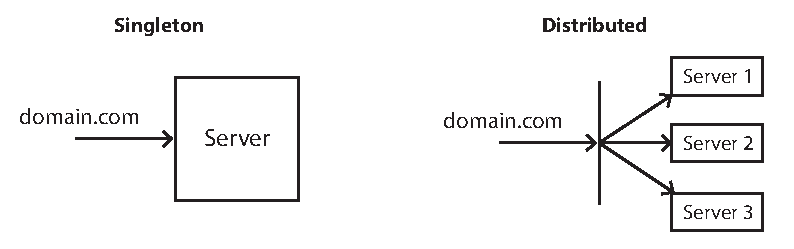
\includegraphics[width=\textwidth]{gfx/server_solutions.pdf}
    \caption{Illustration of a singleton and distributed server solution.}
    \label{fig:server_solutions}
\end{figure}

Distributed server solutions contain several servers possibly on several locations, meaning that DoS will be harder to perform, since there is no single point of failure.
However, this solution cannot ensure consistency and adds complexity.
The two solutions are graphically displayed in Figure~\ref{fig:server_solutions}.
A singleton solution has been chosen due to; consistency and simplicity.
This singleton solution will be denoted as Master or \deno{M}.

The application is required to handle communication with drones, as defined by \at{1} in Figure~\ref{tab:acceptance_tests1}.
In case of the communication being disabled, this might end up with a drone crash.
The technical limitations of antennas for digital wireless communication, sets a constraint for the availability of drones.
Assuming there exists no antenna to cover the physical area of our problem domain, it is necessary to have a distributed antenna setup in order to cover the whole physical area of the problem domain.
This leads to the structure shown in Figure~\ref{fig:antenna_structure}.

\begin{figure}[htb]
    \centering
    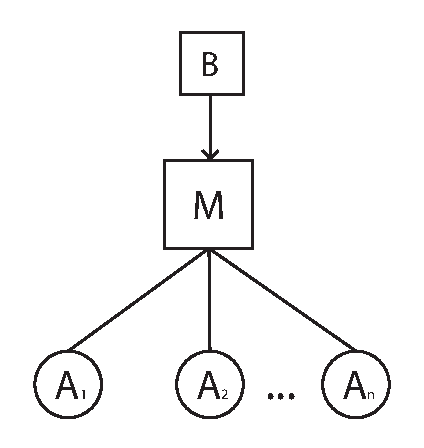
\includegraphics[width=0.5\textwidth]{gfx/antenna_structure.pdf}
    \caption{Antenna structure.}
    \label{fig:antenna_structure}
\end{figure}

If all \deno{B}'s communication with the drones goes through \deno{M}, this would create a single point of failure.
This means that, if \deno{M} crashes at any point, all communication with the drones will be disabled.
Providing the antennas with processing power and opportunity to communicate directly with \deno{B} would solve this issue.
If an antenna crashes only the drones connected to that antenna would be disconnected, leaving the drones connected to other antennas untouched.
This could be achieved by distributing some of the communication from \deno{M}.
This is solved by combining the antennas with distributed processing units, which will be denoted as Slaves or \deno{S}, as shown in Figure~\ref{fig:slave_structure}.

As \deno{S} has a dynamic network position relative to \deno{M}, this enforces that \deno{B} is not able to communicate directly with \deno{S} before getting network information about \deno{S} from \deno{M}. This communication is illustrated by a dashed line in Figure~\ref{fig:slave_structure}.

\begin{figure}[htb]
    \centering
    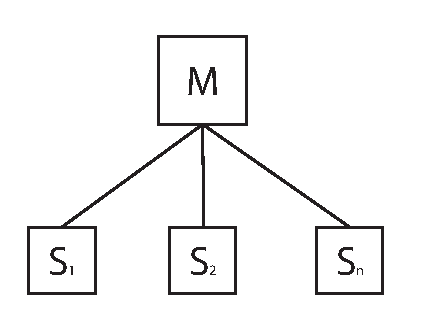
\includegraphics[width=0.5\textwidth]{gfx/slave_structure.pdf}
    \caption{Slave structure.}
    \label{fig:slave_structure}
\end{figure}

The acceptance tests, e.g. 17, 24, 25 in Figure~\ref{tab:acceptance_tests2}, enforces a constraint that requires \deno{M} to be able to store data based of the interaction of the user.
As requests can happen asynchronously, this makes it ideal to use a database denoted \deno{DB}, due to its transaction system in order to ensure no data loss.

The response output of \deno{M} needs to be dynamic based on the user, e.g. Acceptance test 2 in Figure~\ref{tab:acceptance_tests1}, which requires \deno{M} to be capable of processing data and store it in the database.
The processing unit that creates the dynamic response will be denoted \deno{W}.
The communication with the drones are handled by another processing unit, denoted \deno{D}.
If \deno{W} were to handle requests from \deno{S} and \deno{B}, this would increase the load on \deno{W}.
By creating multiple request handlers, it is possible to have a process for each. \deno{W}, \deno{DB}, and \deno{S} are processes, seen in Figure~\ref{fig:daemon_structure}, which improves resource management.
The resource management could be to constrain processing power for each process, or distribute the processes on individual machines.

\begin{figure}[htb]
    \centering
    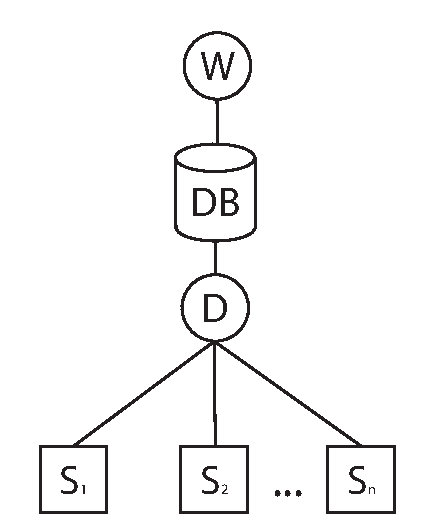
\includegraphics[width=0.5\textwidth]{gfx/daemon_structure.pdf}
    \caption{Daemon structure.}
    \label{fig:daemon_structure}
\end{figure}

% The architecture of \projectname{} differs from other web applications due to the fact that there exists two different type of servers.
% The architecture can be seen in figure~\ref{fig:system_architecture}.
% The server where the web application is running is called Master denoted M.
% For each drone in the system there is a Slave denoted S.
% On both M and S there exists daemons which is responsible for different tasks, however there is some similarity in the tasks they perform.
% These tasks can happen at anytime therefore the program needs to be running at anytime. These daemons are denoted D.
% Each user have a browser they view the application through this is denoted B.
% It is M's responsibility to communicate with every S in the system.
% S is responsible for all communication with the drone it is parred with.

% When a user wants to interact with a drone in the system a session key is needed.
% Such a session key is generated by S and then given to B through M.
% When both B and S have the same session key it is possible for them to communicate without M.
% This ensures that M does not become a bottleneck for controlling and streaming from drones and it reduces latency.
% When a new drone is added it is controlled by its S. This ensures that the system can scaled out and not have to scale up.
% Scale out means using more than one server where scale up means adding more processors, ram etc. to the server so it can handle more by itself.
% M does not handle commands and streaming, and every drone in the system have their own S.
% This makes the application architecture scalable because it removes bottlenecks from both M and S's.

% \begin{figure}[htb]
%     \centering
%     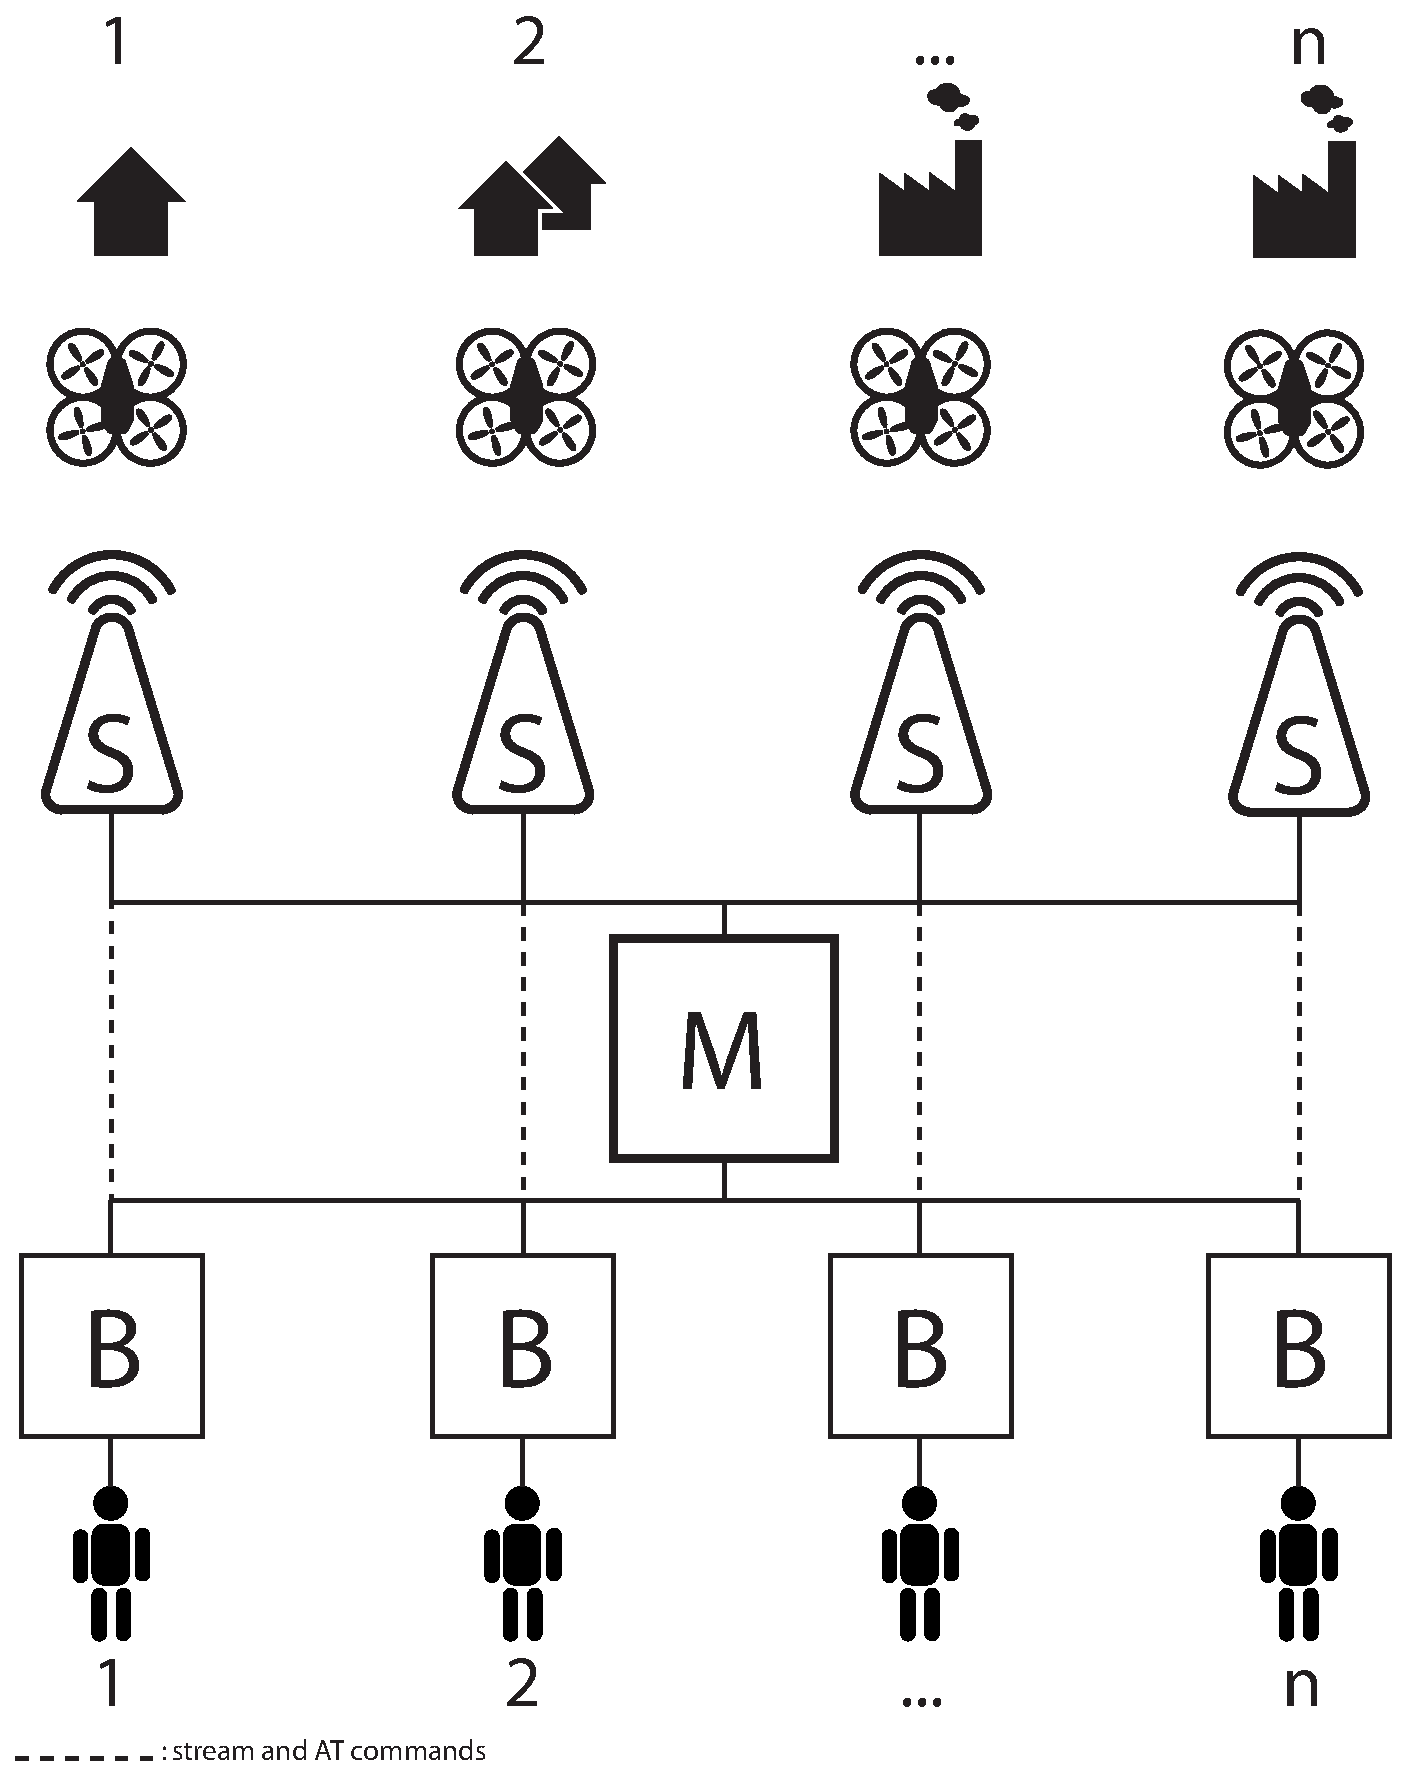
\includegraphics[width=\textwidth]{gfx/system_architecture.pdf}
%     \caption{System architecture of \projectname{}}
%     \label{fig:system_architecture}
% \end{figure}

% The system only uses one M. This can also be seen the bottleneck of the system.
% If M crashes all S's and B's will have to wait for M to come back up.
% One alternative could be running with more M's and in that way scale out.

% There is always one S for each drone connected to the system.
% In this way the system is scaled out.
% This ensures that any S is not likely to become a bottleneck.
% This was done because the drone uses wireless network which is short ranged and the drone is the host which means that the server needs one wireless connection for each drone it have to transmit to.
% One alternative could be only running with one S at each company and just scale it up.
% The problem with this is the server will need a wireless connection for each drone it have to control and it have to be in range.

% Daemon is a background process on a Linux system.
% Daemons are used when it is needed that a process is running at all times.
% In \projectname{} there are both the session key system which both resides on M and S and a policy file system for Adobe Flash on S.
% Both of these processes needs to be running at all times for the user to interact with the drone on S.
\section{Functionality distribution}\label{sec:functionality_distrubution}
% Hvilke funktionaliteter skal dækkes?
% Hvilke instancer dækker hvad?
% Hvorfor gør de det?

The functionality of the system can be derived from the acceptance tests.
This section will cover what instances are responsible for each functionality.

The need for storing data is derived from \at{1}, as previously described this is handled by the database \deno{DB}, which is a part of \deno{M}.
\at{2} sets the need for a dynamic response to \deno{B}, which requires processing of the stored data.
This processing is handled by Web or \deno{W} as the structure contains a singleton server solution.

Knowing that \deno{S} has a dynamic location relative to \deno{M}, this requires \deno{S} to send a signal to the daemon or \deno{D} in order for \deno{M} to get the location of \deno{S} on the network.
\deno{D} is then responsible for being able to receive incoming signals from \deno{S}.

Displaying video is required of \deno{B} by \at{3}.
The video displayed by \deno{B} is a stream, which requires that \deno{S} sends out a video stream.
In order to control a drone, commands have to be provided to the drone, as required by \at{3}.
\deno{S} is responsible for being able to receive commands and have the drone execute the given command.
\at{29} enforces security of the command handler.
\deno{S} is the only instance with a direct link to the drone, this makes \deno{S} responsible for the command handler's security.

% While Section~\ref{sec:application_structure} covered the overall structure of this application, this section will cover how the functionality is divided between the Master and the Slaves in the system. \\

% The Master is the users only way into the system.
% This access will always be via the users local web browser, where he sees the web system for \projectname{}.
% This web system and the database containing all informations about the system, drones, users etc. will be located on the Master.
% The Master is responsible for providing these services and coordinating the communication between the users and drones via the Slaves. \\

% A Slave is needed for every drone in the field, as the drones are not capable of long-distance communication.
% Therefore, in order to communicate with any drone, the communication must be channeled through its assigned Slave.
% This Slave is responsible for keeping contact with the drone and communicate directly with it via its API's.



\section{Communication network}\label{sec:communication_network}

Having functionality distributed across several instances sets the need for communication between the instances.
Based on Figure~\ref{fig:slave_structure}, which displays the dependency between \deno{B}, \deno{M}, and \deno{S} this leads to the diagram shown in Figure~\ref{fig:dataflow_diagrem}. \\


\begin{figure}[!h]
    \centering 
    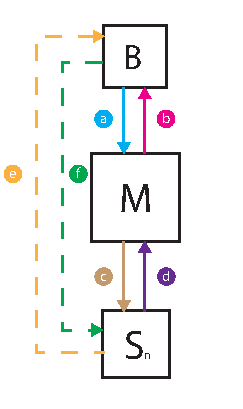
\includegraphics[width=0.5\textwidth]{gfx/dataflow_diagram.pdf}
    \caption{Dataflow diagram of \projectname{}}
    \label{fig:dataflow_diagrem}
\end{figure}


The arrows represent a connection, each connection represent dataflow in the direction of the arrow.
The type of data flowing in each connection and the reasons behind will be covered as each connection is discussed below. \\

Connection \deno{a} covers requests made by \deno{B}, which covers HTTP requests, which is a limit of web solutions that they must use the HTTP protocol.
HTTP requests enable the user to view the web application through his browser, and to send information.
In order to fulfill the request created by \deno{a}, a response is needed which the connection \deno{b} handles.
This connection covers the flow of the dynamic content created by \deno{M}, and static content such as: images, stylesheets, and multimedia objects.
Connection \deno{b} sends both the static and dynamic content back to \deno{B} to be displayed for the user. \\

The connection \deno{d} handles the signal described in Section~\ref{sec:functionality_distribution}.
This signal covers the initial communication between \deno{S} and \deno{M}. \deno{M} verifies the identity of \deno{S} by \deno{S} sending its own unique identifier.
This unique identifier is a string, which consist of X characters \fixme{How many chars?}.
All unique identifiers of each \deno{S} is known to \deno{M}.
This allows \deno{M} to determine the identity of each incoming signal. When \deno{M} receives a signal, and verify the identity of \deno{S}, the source location of the signal is stored in \deno{M} making \deno{M} able to know the location of \deno{S}. \\

Since requests from \deno{B} can happen asynchronously and from dynamic locations, it can create a problem that the identity of the connection made from \deno{S} to \deno{f} is not known. 
\at{28} sets the requirement of differentiating between incoming connections to \deno{S}.
If the communication described in connection \deno{e} and connection \deno{f} were running through \deno{M}, this would be no problem as security would be handled by the already existing sessions on \deno{M}.
The connections \deno{e} and \deno{f} are required to transport a large amount of data.
This data covers a video feed of the drone's video camera and commands for the drone.
This would increase the load on \deno{M}, which is not desired as \deno{M} is assumed to have a high load already.
However, since connection \deno{e} and connection \deno{f} are not running through \deno{M}, this leaves the problem of which \deno{B}, \deno{S} should listen to. \\

The solution chosen to solve this problem is to make \deno{S} create a randomly generated key (session key), that contains 40 characters and is unique relative to \deno{S} stored on \deno{S} itself.
When \deno{S} receives incoming commands, \deno{S} verifies whether or not the key received along with the command is equal to the one locally stored on \deno{S}.
If this is the case, \deno{S} classifies the received command as valid and performs the action.
The session key is delivered to \deno{B} from \deno{M}, as \deno{M} is able to verify the identity of \deno{B} through the session. \\

The connection \deno{c} covers requesting a session key by \deno{M}.
As \deno{M} has a static location, \deno{S} is able to verify the identity of \deno{M} based on its location.
Connection \deno{d} covers the response of the request received in \deno{c}, and \deno{M} is able to verify the identity of \deno{S} based on its location. \\

\begin{figure}[!h]
    \centering 
    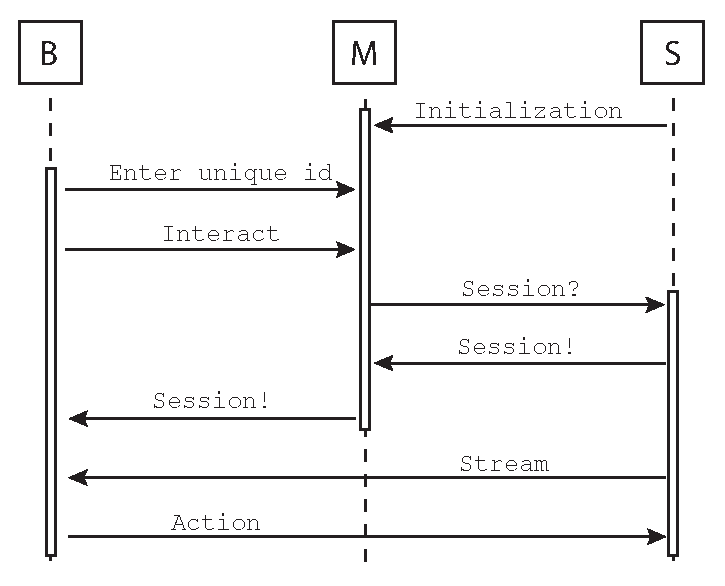
\includegraphics[width=\textwidth]{gfx/sequence_diagram.pdf}
    \caption{Sequence diagram of the communication network between \deno{B}, \deno{M}, and \deno{S}}
    \label{fig:sequence_diagram}
\end{figure}
\fxfatal{Check UML notation.}


The functionalities of the described connections, can only happen in a sequence as illustrated in Figure~\ref{fig:sequence_diagram}.
Each message in the sequence diagram can be done multiple times, however above messages are enforced to be performed atleast once in order for the given message to be performed. \\


% The communication network is crucial for \projectname{} to work.
% When designing a scalable communication network it is important to choose the right structure.
% There are different ways when designing such a network but identical for them all is that they need to support the structure of \deno{M}, \deno{S} and \deno{B} described in section~\ref{sec:application_structure}.

% One solution is to make a structure where \deno{M}, \deno{S} and \deno{B} talk to each other with a level of security. 
% The security aspect would be implemented with a form of session key. 
% This key would be used to determine if a session between a \deno{B} and a \deno{S} is valid.
% Another solution is to provide no security aspect and let it be up to the users and / or company to keep drones safe from intruders.
% This would lessen the communication between \deno{B}, \deno{M} and \deno{S}.  
% It would also decrease the load on \deno{M} and \deno{S}'s database. 
% On the down side the system could be considered not safe because it would be possible to tamper with the drones.
% As this is a system where it is important that the integrity is high, evidence is not tampered with, and where the outcome of an unauthorized user controller a drone could be devastating, it is important to deliver some form of security.



% This lead to a solution where sessions is designed to keep the integrity and secure evidence as seen in figure~\ref{fig:sequence_diagram}. 
% As seen in the figure there is designed a level of security because of the sessions.
% It is not possible for a \deno{B} to interact with a drone without having a session with a drones \deno{S}.

% When a drone is purchased a \deno{S} is setup at the location where the drone is going to operate.
% The \deno{S} sends an initializing message to \deno{M}, informing \deno{M} that a new drone has entered the system.
% \deno{M} adds the drone with the IP and location of the \deno{S}, along with the drone's unique identifier.
% If \deno{M} receives an initializing message from a \deno{S} with a drone identifier that is already in the system, it will destroy any session that correlates with that drone.
% The sessions is destroyed because if one or more sessions are granted and \deno{S} sends its initializing message it is safe to assume that \deno{S} either disconnected or crashed and all sessions keys are invalid.
% Furthermore if the IP of \deno{S} differs from the IP \deno{M} holds in its database it will be updated.

% If a user tries to interact with a drone the system behaves differently.
% A session key will be made on a \deno{S}, this key will be send to \deno{M} and giving to \deno{B}. If this session key is valid it is possible for the user to communicate directly with \deno{S} without \deno{M}.

% \begin{figure}[!h]
%     \centering 
%     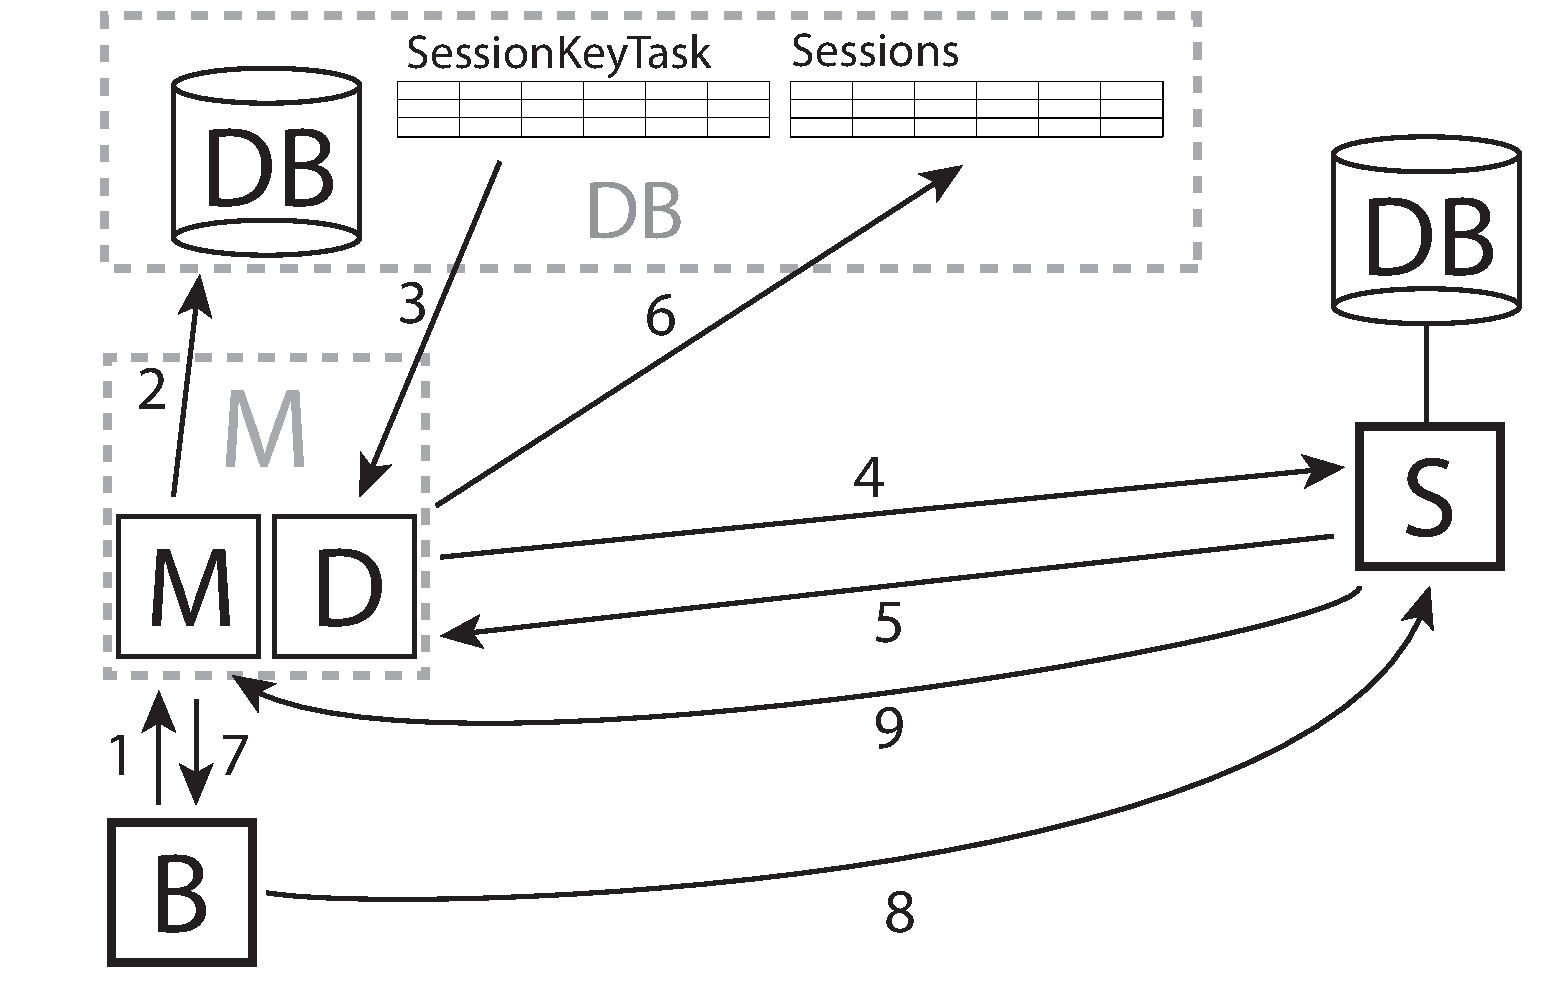
\includegraphics[width=\textwidth]{gfx/sessionkey_communication.pdf}
%     \caption{Session key communication between \deno{B}, \deno{M}, and \deno{S}}
%     \label{fig:sessionkey_communication}
% \end{figure}

% This behavior can be seen in figure~\ref{fig:sessionkey_communication}. 

% Session keys have been designed for security reasons.
% Firstly they were designed to ensure that only one user at a time can control a drone.
% Secondly it ensured that unauthorized users do not have the possibility of controlling a drone.

% \begin{enumerate}
% 	\item Request send from \deno{B} to \deno{M} about getting a session key to interact with a drone.
% 	\item \deno{M} inserts this request in its database table called SessionKeyTask.
% 	\item \deno{D} scans the database table SessionKeyTask, when it sees a new entry it select it and then deletes it from the table.
% 	\item \deno{D} requests a session key from \deno{S} parred with the drone the user wants to interact with.
% 	\item \deno{S} makes a random generated string with uppercase, lowercase letters and number. This string is used as the session key. \deno{S} updates its database with this session key and then sends it back to \deno{D} on \deno{M}.
% 	\item \deno{D} inserts the newly received session key into the session table of \deno{M}.
% 	\item \deno{M} then contacts \deno{B} with the session key.
% 	\item \deno{B} uses this session key to access \deno{S} and through it interact with the drone.
% 	\item A Timeout happens if \deno{B} and \deno{S} does not communicate for 10 seconds.
% \end{enumerate}

% Communication between the servers in the system is crucial. 
% Therefore it is important design a method or a set of methods handling the communication between them. 
% One method could be to make a service which handles all these requests on each server.
% The problem however is that using a single service might create a bottleneck.
% An alternative solution is to make a service for each communication level.
% One service that handles sessions, a service that handles control commands, and a service that handles initial messages from \deno{S} see section~\ref{sec:application_structure}.\fxfatal{Den her paragraf er uspecifik}

% This lead to a solution where the different actors in the system delivered and / or depended on services.

% The interface of the communication network can be seen in figure~\ref{fig:communication_network}.

% The communication network of \projectname{} uses four different ports for providing its services:

% \begin{itemize}
% 	\item Port A - service port for sending and receiving drone control commands.
% 	\item Port B - service port for receiving and sending initial messages.
% 	\item Port C - service port for sending and receiving session information including session keys.
% 	\item Port Web - service port for sending and receiving web specific information.
% \end{itemize}

% \begin{figure}[!h]
%     \centering 
%     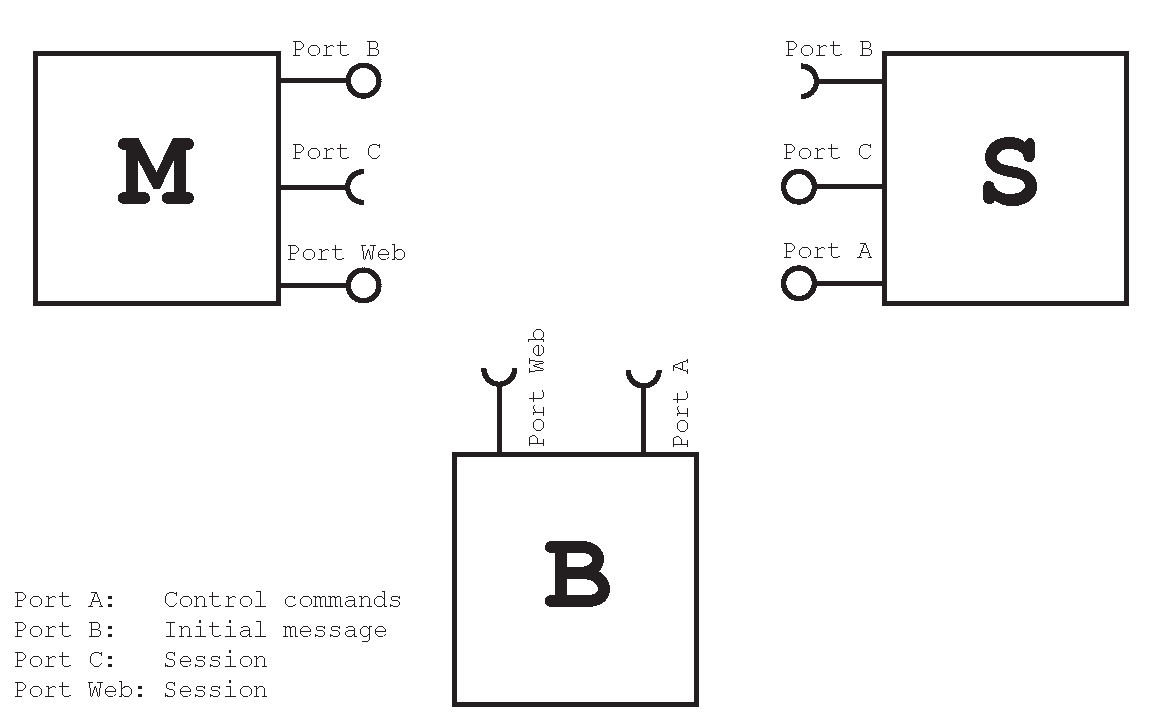
\includegraphics[width=\textwidth]{gfx/communication_network.pdf}
%     \caption{Communication network between \deno{B}, \deno{M}, and \deno{S}}
%     \label{fig:communication_network}
% \end{figure}

% When designing a communication network it is also important to select the right technique for exchanging data between services.
% One of the more widely used techniques are Extensible Markup Language.
% Extensible Markup Language, or XML for short, is a markup language designed to easily mark up data.
% The markup that XML provides makes it possible to easily send and receive data.
% The Extensible in XML makes it possible to extent what data types XML can handle through the XML schema. \citep{simonstl}
% This gives XML a drawback because XML is designed to be extensible it also carries a lot of overhead when used to mark up data.

% \projectname{} needs to be scalable therefore it is important to use as little overhead when sending structured information.
% Otherwise there is a chance that this overhead creates a bottleneck within the network.

% JSON, or JavaScript Object Notation, is design for data interchange and to be human-readable.
% It have a simpler syntax than XML and is not build to be extensible, it is not even a markup language. 
% It is a structured way of exchanging data between sources. 
% This results in less overhead i.e. it costs less data for each piece of information. 
% JSON is also data orientated which makes it easier to map a JSON object directly to a object orientated structure.
% Douglas Crockford call JSON ``The Fat-Free Alternative to XML'' \citep{JSON}.

% Therefore JSON is the perfect format for data interchange between the different services in \projectname{}. There are lesser costs associated with JSON than XML and it is easier to map them into a object orientated language.
\section{Object Model}
\label{section:uml_notation}
\label{subsec:objects}

This section will cover the design choices behind the application's object model, derived from the use cases in Section~\ref{sec:use_cases}.
The UML object model diagram can be seen in Figure~\ref{fig:UML_class_diagram}, and is guided by the UML standard guide written in cooperation by several different software companies~\citep{UML_notation}.\\

The UML attribute notation in this report is:
\begin{itemize}
    \item PK attribute - means that the attribute is a primary key.
    \item FK attribute - means that the attribute is a foreign key.
    \item attribute : type - all attributes will have a type e.g. \verb+id : int+.
\end{itemize}

The system will contain the following objects: \deno{Affiliate Privilege}, \deno{Company}, \deno{Drone}, \deno{Privilege}, \deno{Role}, \deno{Session}, and \deno{User}.
The model of the objects and their relationships can be seen in Figure~\ref{fig:UML_class_diagram}.
Each object covered is represented in the object model diagram with its name in lowercase and pluralized, e.g. \deno{User} object $\rightarrow$ \deno{users}.
If an object's name consists of several words the spaces will be replaced by underscores, e.g. Session Key Task becomes session\_key\_tasks.
The relationships between objects can either be implicit with a line directly from one object to another, or explicit with a simple or rich relationship model between the two objects.
Simple relationship models are models without a PK.
They are represented in the model diagram with both objects in lowercase and pluralized, e.g. roles\_users.
Rich relationship models have a PK.
This kind of relationship model does not have a predetermined naming convention, therefore it can be anything as long as it does not collide with the other model names, e.g. user\_privileges.\\

\begin{figure}[htb]
    \centering
    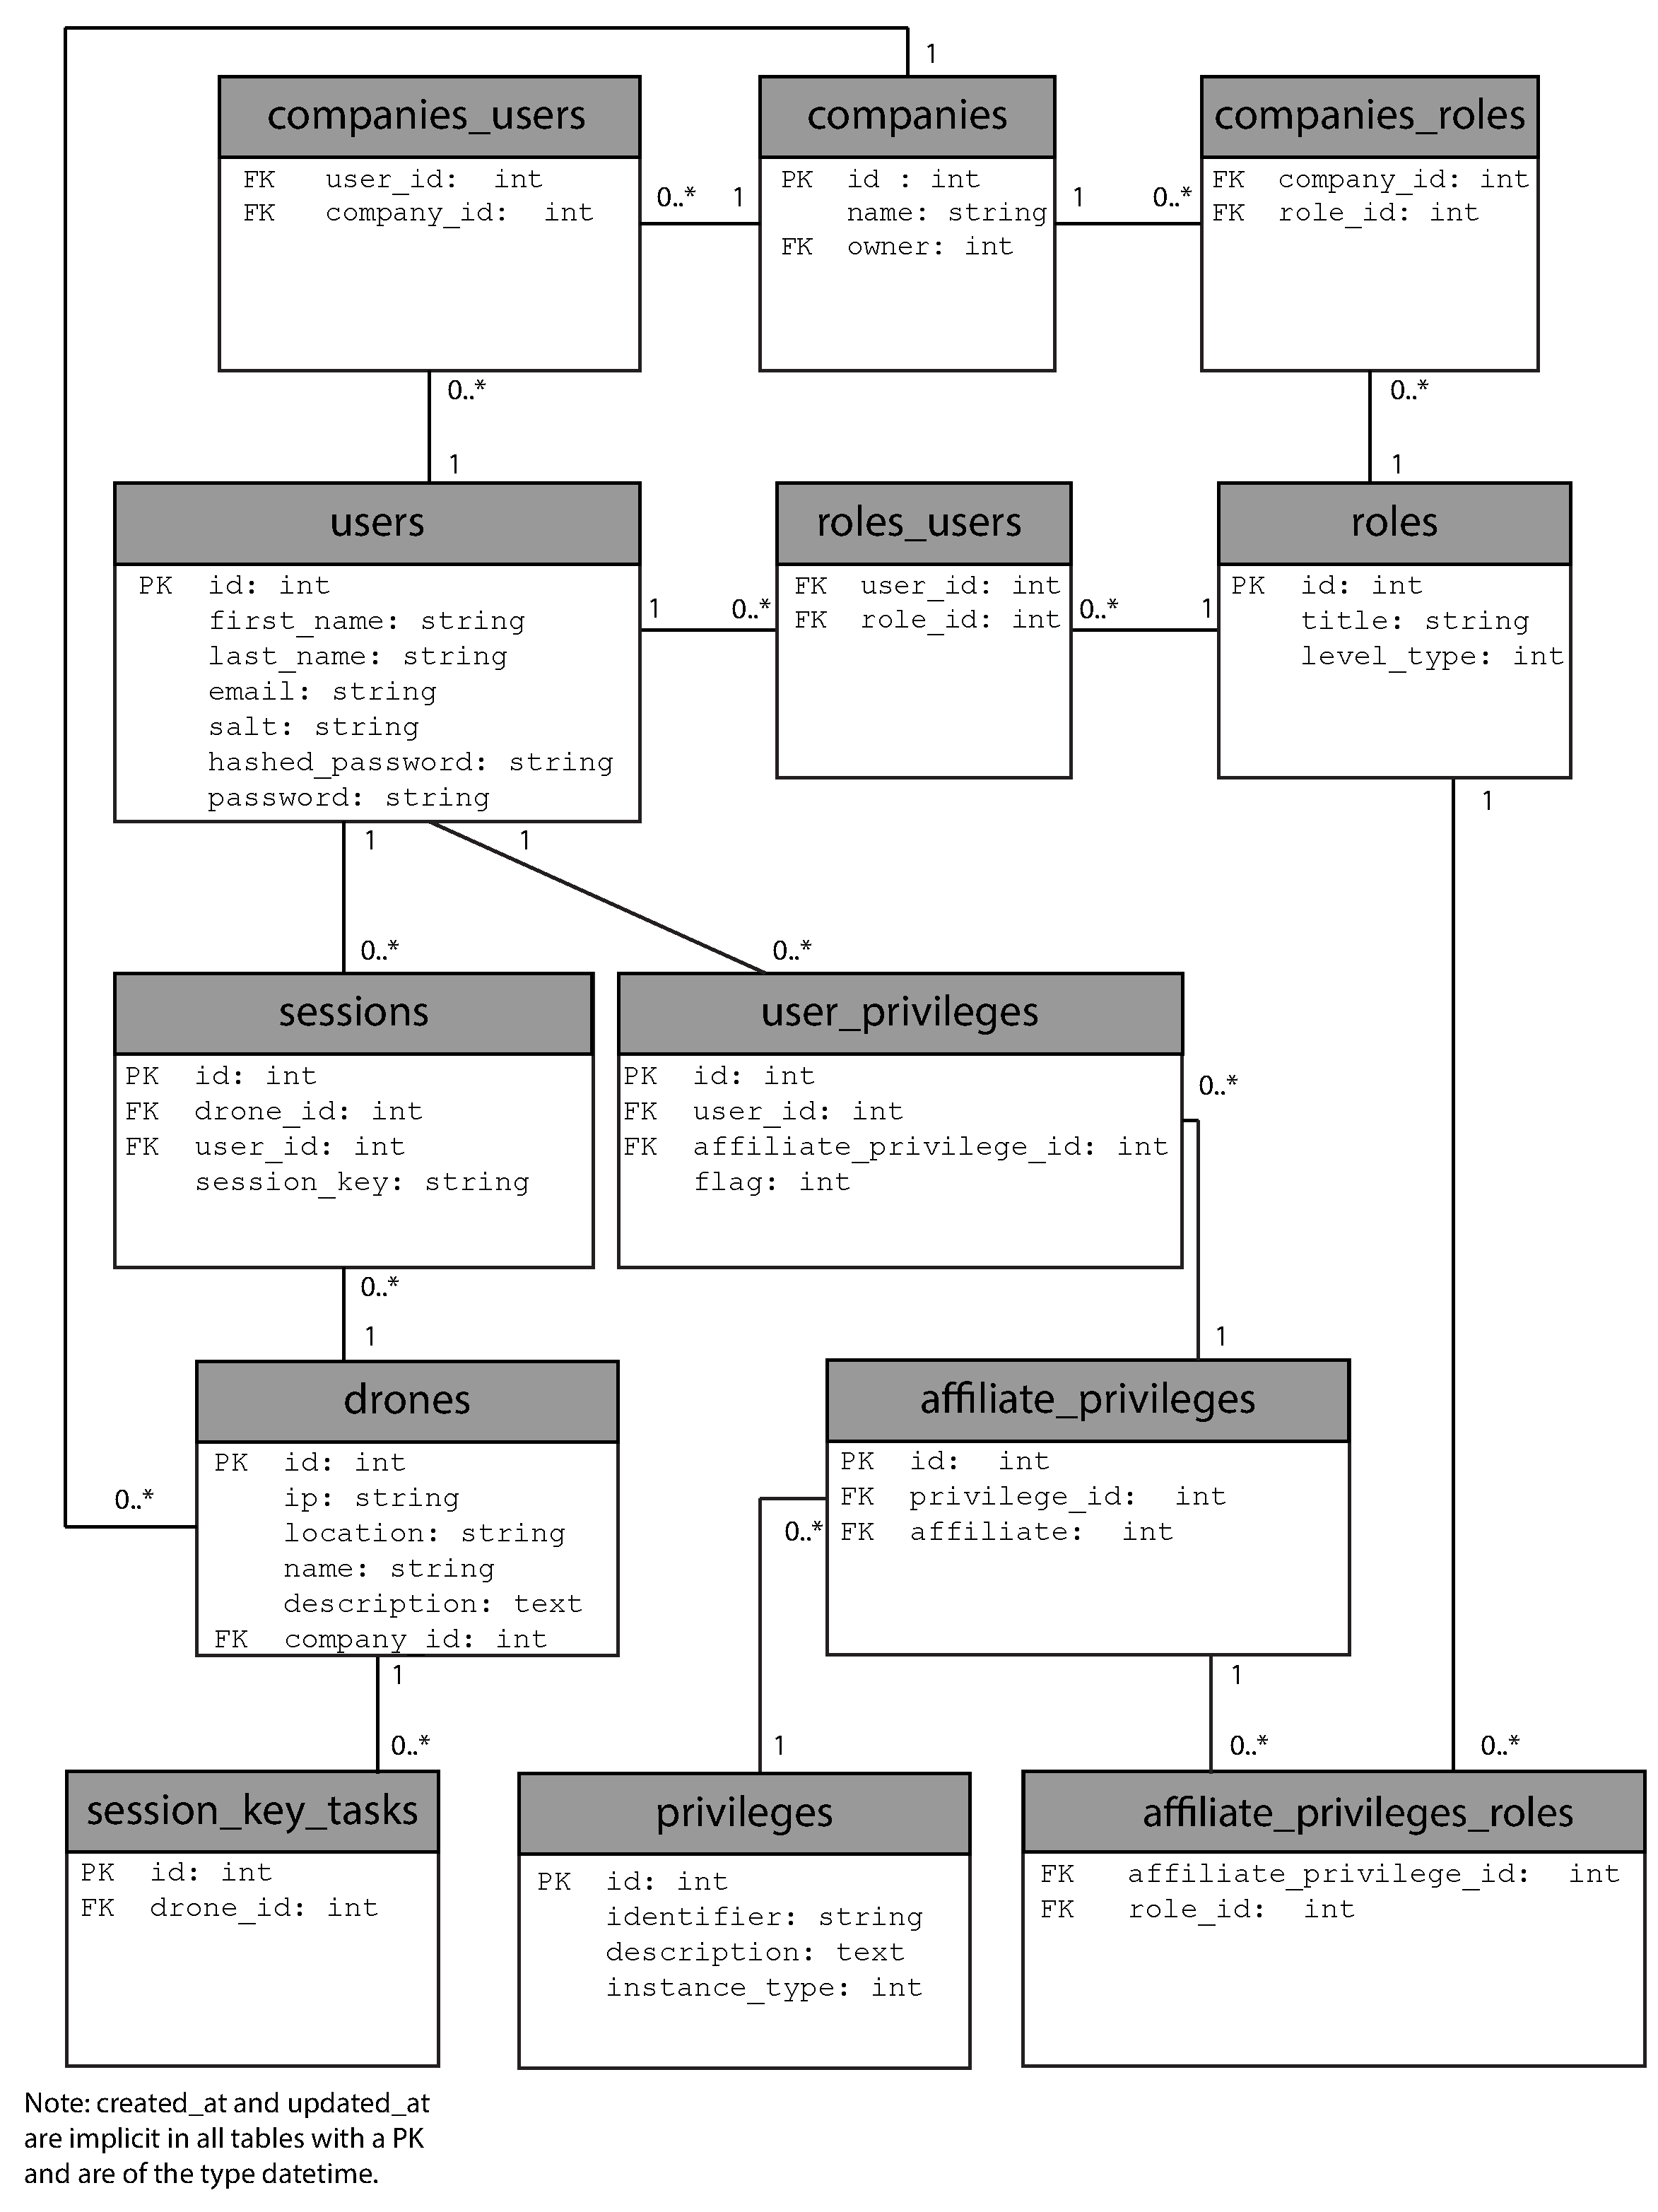
\includegraphics[width=0.95\textwidth]{gfx/UML_model.pdf}
    \caption{UML Class Diagram of \projectname{}}
    \label{fig:UML_class_diagram}
\end{figure}


\subsection{Objects}\fixme{Skal denne overskrift være der? Det burde ikke være nødvendigt at have den, men så skal teksten ændres lidt.}
Access to and actions of the system is restricted.
This restriction is based on the identity of user in the system.
An instance of the \deno{User} object represents a user to the system.
The \deno{User} object has the attributes \verb+email+ and \verb+password+, as seen in Figure~\ref{tab:user_object} in Appendix~\ref{app:objects}, these combined form the login credentials needed for a user to authenticate his identity towards the system. \\

The \verb+email+ is publicly available, which leaves the \verb+password+ to be protected in order for user to protect his identity in the system.
The \verb+password+ entered by the user is concatenated with a \verb+salt+ and hashed through a SHA-1 hashing algorithm to be stored in \verb+hashed_password+.
The hashing algorithm provides a way for storing the password without having its exact value, as this could leave to a security flaw.
Having access to passwords of users directly, e.g. through a hacker attack, would allow the hacker to login into the users account, which is unintended for the system.
When a salt is concatenated before hashing it makes it harder for the hacker to gain the original passwords, e.g. through a rainbow table~\cite{something}. \\

Having a distributed setup with multiple \deno{S}, each representing a \deno{Drone} object, means that the network locations of these need to be known in order to communicate.
The network location is stored in the \verb+ip+ field of the \deno{Drone} object, as shown in Figure~\ref{tab:drone_object} of Appendix~\ref{app:objects}.
The physical drone have a unique identifier known as \verb+name+, which makes the user able to identify a given drone. \\

The users of the system will be part of different companies, therefore there is a need for grouping users by a company.
The \deno{Company} object have an \verb+owner+, which is a reference to a \deno{User} object.
This is required for the system to know which user have access to all \deno{Affiliate Privilege} objects of the company. \\

An \deno{Affiliate Privilege} object references a \deno{Privilege}, and only when combined they form a unique key.
This key unlocks a certain functionality, meaning that if the user does not have a relation to the \deno{Affiliate Privilege} object, which represents the key, then the user is not able to unlock that functionality.
\deno{Role} objects give the possibility of grouping \deno{Privilege} objects together.
Each \deno{Company} have a related role which contains all privileges, of which the company have full control.
Full control gives the right for passing on a privilege, or disabling if the privilege is already granted.
\deno{Affiliate Privilege} objects have a field \verb+affiliate+ that links the privilege to an object of the type declared by the referenced \deno{Privilege} object's \verb+instance_type+ field. \\

The \deno{Session} object represents an active pilot connection between a user and a drone.
The \verb+session_key+ field provides a key that needs to be sent along with the commands.
The \deno{Session Key Task} object is an object used for \deno{D} and \deno{M} to communicate through \deno{DB}, as shown in Figure~\ref{fig:daemon_structure} in Section~\ref{sec:application_structure}. \\

In Section~\ref{sec:privileges} solutions for handling privileges were discussed.
From this discussion it was decided to model a system capable of handling all proposed solutions to fit scenarios of the users.
The \deno{User Privileges} relationship allows for connecting individual {Privilege} objects to a \deno{User} object.
This is could be either granting or revoking, i.e. exceptions, the privilege.
The \verb+flag+ field represents a value of either 1 or -1; 1 is regarded as granted, and -1 is regarded as revoked.


% \subsection{Relationships}
% The system is designed with flexibility and scalability in mind, and the structure of Roles and Privileges are what provides those features.
% As described before there are two ways that a User can be granted a specific Privilege.
% These are by 1) getting the Privilege granted directly via the \verb+User_Privileges+ table or 2) by being a member of a Role that via the \verb+Privileges_Roles+ table that has one or more Privileges granted.
% These will be explained in details in the following subsections.


% % Users and Privileges %
% An administrator can grant a specific Privilege directly to a user via the \verb+User_Privileges+ table.
% This Privilege is then affiliated with an object -- usually a Drone.
% The Privilege could also be a system functionality, however, as described in Section~\ref{sec:privileges}. \\

% This relationship is also used for exceptions.
% In an example where five Users: U1, U2, U3, U4 and U5 are a member of a Role: R1, we may have a situation where U2 is not suppose to have access to a given Privilege P1 in R1.
% Then a User-specific Privilege is granted to U2 on P1, but with the ``exception''-flag marked.
% This is equal to blacklisting U2 from using Privilege P1, providing the system with a lot of flexibility, as even though a group of Users are granted a number of Privileges via a role, User-specific exceptions can be added to this setting. \\


% % Roles and Privileges %
% As mentioned before -- the reason that Roles can be used to assign Privileges to a User, is to make both the administration and data structure of Users and Privileges as simple and efficient as possible.
% By allowing exceptions, full flexibility is still possible. \\

% This is how the relationship between Roles and Privileges works: \\

% An administrator creates a Role.
% Lets call this Role ``Control Drone \#4''.
% A number of Privileges are assigned to this Role.
% It could be the following:

% \begin{itemize}
%     \item Watch the video feed from a specific drone
%     \item Control the movement of a specific drone
% \end{itemize}

% Those Privileges are then linked to this Role and to the Drone this concerns. \\

% Roles can be assigned with affiliation to both Users and Companies.
% Say a user \verb+U1+ needs access to Drone \#4.
% User U1 then needs to either have the Privileges directly granted or be a member of the role ``Control Drone \#4''.


% % Privileges and granting of Privileges %
% Since it is possible to grant Privileges both directly to a User and via a Role, the same Privilege can be used in more than one context.
% Therefore the \verb+Affiliation_Privileges+ table exists.
% This table links the granting of a Privilege with the actual Privilege and defines on which Object the Privilege applies.
% The reason for having this table and not just link the two granting-tables \verb+User_Privileges+ and \verb+Privileges_Roles+ directly to the \verb+Privileges+ table, is that we try to avoid redundant data by having the data in the \verb+Privileges+ and \verb+Affiliation_Privileges+ table make up one instance of a privilege together.
% This is then granted to a User or a Role, who can then use the Privilege. \\

% The system is designed so that any User can grant a Privilege he already has already been granted to another User if he is permitted to.
% This is controlled via a ``re-grantable'' flag which is set in either the \verb+User_Privileges+ table or the \verb+Privileges_Roles+ table.
% By marking this flag as ``true'', the User or Users that via a Role is granted the Privilege in question, can via an interface in the system re-grant the Privilege to other Users in the same Company.


% %Note: Alle brugere kan videregrante et privilege hvis de har tilladelse til det. Det er et flag som sætes i user_privileges og privileges_roles, som tillader alle der har dette privilegie til at videregrante det. Husk at beskrive hvordan et privilege og et affiliation privilege til sammen giver et grant-able privilegie


% % Privileges and Drones %
% With \projectname{} in its current form, most Privileges that are granted will have an connected with a Drone.
% Privileges and its a affiliations are linked in the \verb+Affiliation_Privileges+ table.
% This is also where Drones are linked to any granted privilege. \\

% As described earlier, Drones are the current object-type implemented in the system.
% However, the structure and model of the system allows for later expansion, connection new objects such as stationary cameras or any other type of object to the system.
% The \verb+Affiliation_Privileges+ has a third field named \verb+object_id+.
% This field links the Privilege, the granting of it and the Object that this granting is valid for. \\

% An example could be linking Privilege P1, User U1 and Drone D1.
% Say P1 is the privilege for watching the video feed of a drone.
% Then the user U1 will have access to watch the video feed of Drone D1.


% % Drones and Companies %
% The \verb+Company_drones+ table defines a relationship between a Drone and a Company.

% The administrator of each Company defines the Roles in that Company.
% In doing so, he defines which Privileges that are granted in every Role.
% These Privileges are linked to a (Drone)-object.
% The system must make sure that any Company administrator cannot link a Privilege with a Object that is not within his control. \\

% This relationship defines which Drones are available to each Company.
% When a Company administrator adds new Roles (and hence Privileges), he is only able to associate it with Drones that are connected to the Company in question.

% **************************************************************************************************************
% A Classic Thesis Style
% An Homage to The Elements of Typographic Style
%
% Copyright (C) 2012 Andr\'e Miede http://www.miede.de
%
% If you like the style then I would appreciate a postcard. My address
% can be found in the file ClassicThesis.pdf. A collection of the
% postcards I received so far is available online at
% http://postcards.miede.de
%
% License:
% This program is free software; you can redistribute it and/or modify
% it under the terms of the GNU General Public License as published by
% the Free Software Foundation; either version 2 of the License, or
% (at your option) any later version.
%
% This program is distributed in the hope that it will be useful,
% but WITHOUT ANY WARRANTY; without even the implied warranty of
% MERCHANTABILITY or FITNESS FOR A PARTICULAR PURPOSE.  See the
% GNU General Public License for more details.
%
% You should have received a copy of the GNU General Public License
% along with this program; see the file COPYING.  If not, write to
% the Free Software Foundation, Inc., 59 Temple Place - Suite 330,
% Boston, MA 02111-1307, USA.
%
% **************************************************************************************************************
% Note:
%    * You must not use "u etc. in strings/commands that will be spaced out (use \"u or real umlauts instead)
%    * New enumeration (small caps): \begin{aenumerate} \end{aenumerate}
%    * For margin notes: \marginpar or \graffito{}
%    * Do not use bold fonts in this style, it is designed around them
%    * Use tables as in the examples
%    * See classicthesis-preamble.sty for useful commands
% **************************************************************************************************************
% To Do:
%		 * [high] Check this out: http://www.golatex.de/koma-script-warnung-in-verbindung-mit-listings-package-t2058.html
%    * [medium] mathbb in section-titles/chapter-titles => disappears somehow in headlines!!!
% **************************************************************************************************************
\documentclass[ twoside,openright,titlepage,numbers=noenddot,headinclude,%1headlines,% letterpaper a4paper
                footinclude=true,cleardoublepage=empty,abstractoff, % <--- obsolete, remove (todo)
                BCOR=5mm,paper=a4,fontsize=11pt,%11pt,a4paper,%
                ngerman,american,%
                ]{scrreprt}

%********************************************************************
% Note: Make all your adjustments in here
%*******************************************************
% ****************************************************************************************************
% classicthesis-config.tex
% formerly known as loadpackages.sty, classicthesis-ldpkg.sty, and classicthesis-preamble.sty
% Use it at the beginning of your ClassicThesis.tex, or as a LaTeX Preamble
% in your ClassicThesis.{tex,lyx} with \input{classicthesis-config}
% ****************************************************************************************************
% If you like the classicthesis, then I would appreciate a postcard.
% My address can be found in the file ClassicThesis.pdf. A collection
% of the postcards I received so far is available online at
% http://postcards.miede.de
% ****************************************************************************************************

% ****************************************************************************************************
% 1. Configure classicthesis for your needs here, e.g., remove "drafting" below
% in order to deactivate the time-stamp on the pages
% ****************************************************************************************************
\PassOptionsToPackage{eulerchapternumbers,listings,drafting,%
				 pdfspacing,%floatperchapter,%linedheaders,%
				 subfig,beramono,eulermath,parts}{classicthesis}
% ********************************************************************
% Available options for classicthesis.sty
% (see ClassicThesis.pdf for more information):
% drafting
% parts nochapters linedheaders
% eulerchapternumbers beramono eulermath pdfspacing minionprospacing
% tocaligned dottedtoc manychapters
% listings floatperchapter subfig
% ********************************************************************

% ********************************************************************
% Triggers for this config
% ********************************************************************
\usepackage{ifthen}
\newboolean{enable-backrefs} % enable backrefs in the bibliography
\setboolean{enable-backrefs}{false} % true false
% ****************************************************************************************************


% ****************************************************************************************************
% 2. Personal data and user ad-hoc commands
% ****************************************************************************************************
\newcommand{\myTitle}{LONE\xspace}
\newcommand{\mySubtitle}{Lone is Observation of Nondeterministic Environments\xspace}
%\newcommand{\myDegree}{Doktor-Ingenieur (Dr.-Ing.)\xspace}
\newcommand{\myName}{SW701E12\xspace}
\newcommand{\myProf}{Put name here\xspace}
\newcommand{\myOtherProf}{Put name here\xspace}
\newcommand{\mySupervisor}{Put name here\xspace}
\newcommand{\myFaculty}{Put data here\xspace}
\newcommand{\myDepartment}{Put data here\xspace}
\newcommand{\myUni}{Aalborg University\xspace}
\newcommand{\myLocation}{Aalborg\xspace}
\newcommand{\myTime}{December 2012\xspace}
\newcommand{\myVersion}{version 4.1\xspace}
\newcommand{\projectname}{<projectname>}

% ********************************************************************
% Setup, finetuning, and useful commands
% ********************************************************************
\newcounter{dummy} % necessary for correct hyperlinks (to index, bib, etc.)
\newlength{\abcd} % for ab..z string length calculation
\providecommand{\mLyX}{L\kern-.1667em\lower.25em\hbox{Y}\kern-.125emX\@}
\newcommand{\ie}{i.\,e.}
\newcommand{\Ie}{I.\,e.}
\newcommand{\eg}{e.\,g.}
\newcommand{\Eg}{E.\,g.}
% ****************************************************************************************************


% ****************************************************************************************************
% 3. Loading some handy packages
% ****************************************************************************************************
% ********************************************************************
% Packages with options that might require adjustments
% ********************************************************************
\PassOptionsToPackage{latin9}{inputenc}	% latin9 (ISO-8859-9) = latin1+"Euro sign"
 \usepackage{inputenc}

%\PassOptionsToPackage{ngerman,american}{babel}   % change this to your language(s)
% Spanish languages need extra options in order to work with this template
%\PassOptionsToPackage{spanish,es-lcroman}{babel}
 \usepackage{babel}

\PassOptionsToPackage{square,numbers}{natbib}
 \usepackage{natbib}

\PassOptionsToPackage{fleqn}{amsmath}		% math environments and more by the AMS
 \usepackage{amsmath}

% ********************************************************************
% General useful packages
% ********************************************************************
\PassOptionsToPackage{T1}{fontenc} % T2A for cyrillics
	\usepackage{fontenc}
\usepackage{textcomp} % fix warning with missing font shapes
\usepackage{scrhack} % fix warnings when using KOMA with listings package
\usepackage{xspace} % to get the spacing after macros right
\usepackage{mparhack} % get marginpar right
\usepackage{fixltx2e} % fixes some LaTeX stuff
\PassOptionsToPackage{printonlyused,smaller}{acronym}
	\usepackage{acronym} % nice macros for handling all acronyms in the thesis
%\renewcommand*{\acsfont}[1]{\textssc{#1}} % for MinionPro
\renewcommand{\bflabel}[1]{{#1}\hfill} % fix the list of acronyms
\usepackage[footnote,draft,english,silent,nomargin]{fixme}  % final instead of draft produces errors at
                                                            % compile time
                                                            
%Bjarke HS stuff
\newcommand{\todo}[1]{\fxnote{#1}}
\newcommand{\todoi}[1]{\fxfatal{#1}}
\newcommand{\todoI}[1]{\todoi{#1}}

%Rasmus stuff
\newcommand{\figref}[1]{\figurename~\ref{#1}}

% ****************************************************************************************************


% ****************************************************************************************************
% 4. Setup floats: tables, (sub)figures, and captions
% ****************************************************************************************************
\usepackage{tabularx} % better tables
	\setlength{\extrarowheight}{3pt} % increase table row height
\newcommand{\tableheadline}[1]{\multicolumn{1}{c}{\spacedlowsmallcaps{#1}}}
\newcommand{\myfloatalign}{\centering} % to be used with each float for alignment
\usepackage{caption}
\captionsetup{format=hang,font=small}
\usepackage{subfig}
% ****************************************************************************************************


% ****************************************************************************************************
% 5. Setup code listings
% ****************************************************************************************************
\usepackage{listings}
%\lstset{emph={trueIndex,root},emphstyle=\color{BlueViolet}}%\underbar} % for special keywords
\lstset{language=[LaTeX]Tex,%C++,
    keywordstyle=\color{RoyalBlue},%\bfseries,
    basicstyle=\small\ttfamily,
    %identifierstyle=\color{NavyBlue},
    commentstyle=\color{Green}\ttfamily,
    stringstyle=\rmfamily,
    numbers=none,%left,%
    numberstyle=\scriptsize,%\tiny
    stepnumber=5,
    numbersep=8pt,
    showstringspaces=false,
    breaklines=true,
    frameround=ftff,
    frame=single,
    belowcaptionskip=.75\baselineskip
    %frame=L
}
% ****************************************************************************************************


% ****************************************************************************************************
% 6. PDFLaTeX, hyperreferences and citation backreferences
% ****************************************************************************************************
% ********************************************************************
% Using PDFLaTeX
% ********************************************************************
\PassOptionsToPackage{pdftex,hyperfootnotes=false,pdfpagelabels}{hyperref}
	\usepackage{hyperref}  % backref linktocpage pagebackref
\pdfcompresslevel=9
\pdfadjustspacing=1
\PassOptionsToPackage{pdftex}{graphicx}
	\usepackage{graphicx}

% ********************************************************************
% Setup the style of the backrefs from the bibliography
% (translate the options to any language you use)
% ********************************************************************
\newcommand{\backrefnotcitedstring}{\relax}%(Not cited.)
\newcommand{\backrefcitedsinglestring}[1]{(Cited on page~#1.)}
\newcommand{\backrefcitedmultistring}[1]{(Cited on pages~#1.)}
\ifthenelse{\boolean{enable-backrefs}}%
{%
		\PassOptionsToPackage{hyperpageref}{backref}
		\usepackage{backref} % to be loaded after hyperref package
		   \renewcommand{\backreftwosep}{ and~} % separate 2 pages
		   \renewcommand{\backreflastsep}{, and~} % separate last of longer list
		   \renewcommand*{\backref}[1]{}  % disable standard
		   \renewcommand*{\backrefalt}[4]{% detailed backref
		      \ifcase #1 %
		         \backrefnotcitedstring%
		      \or%
		         \backrefcitedsinglestring{#2}%
		      \else%
		         \backrefcitedmultistring{#2}%
		      \fi}%
}{\relax}

% ********************************************************************
% Hyperreferences
% ********************************************************************
\hypersetup{%
    %draft,	% = no hyperlinking at all (useful in b/w printouts)
    colorlinks=true, linktocpage=true, pdfstartpage=3, pdfstartview=FitV,%
    % uncomment the following line if you want to have black links (e.g., for printing)
    %colorlinks=false, linktocpage=false, pdfborder={0 0 0}, pdfstartpage=3, pdfstartview=FitV,%
    breaklinks=true, pdfpagemode=UseNone, pageanchor=true, pdfpagemode=UseOutlines,%
    plainpages=false, bookmarksnumbered, bookmarksopen=true, bookmarksopenlevel=1,%
    hypertexnames=true, pdfhighlight=/O,%nesting=true,%frenchlinks,%
    urlcolor=webbrown, linkcolor=RoyalBlue, citecolor=webgreen, %pagecolor=RoyalBlue,%
    %urlcolor=Black, linkcolor=Black, citecolor=Black, %pagecolor=Black,%
    pdftitle={\myTitle},%
    pdfauthor={\textcopyright\ \myName, \myUni, \myFaculty},%
    pdfsubject={},%
    pdfkeywords={},%
    pdfcreator={pdfLaTeX},%
    pdfproducer={LaTeX with hyperref and classicthesis}%
}

% ********************************************************************
% Setup autoreferences
% ********************************************************************
% There are some issues regarding autorefnames
% http://www.ureader.de/msg/136221647.aspx
% http://www.tex.ac.uk/cgi-bin/texfaq2html?label=latexwords
% you have to redefine the makros for the
% language you use, e.g., american, ngerman
% (as chosen when loading babel/AtBeginDocument)
% ********************************************************************
\makeatletter
\@ifpackageloaded{babel}%
    {%
       \addto\extrasamerican{%
					\renewcommand*{\figureautorefname}{Figure}%
					\renewcommand*{\tableautorefname}{Table}%
					\renewcommand*{\partautorefname}{Part}%
					\renewcommand*{\chapterautorefname}{Chapter}%
					\renewcommand*{\sectionautorefname}{Section}%
					\renewcommand*{\subsectionautorefname}{Section}%
					\renewcommand*{\subsubsectionautorefname}{Section}%
				}%
       \addto\extrasngerman{%
					\renewcommand*{\paragraphautorefname}{Absatz}%
					\renewcommand*{\subparagraphautorefname}{Unterabsatz}%
					\renewcommand*{\footnoteautorefname}{Fu\"snote}%
					\renewcommand*{\FancyVerbLineautorefname}{Zeile}%
					\renewcommand*{\theoremautorefname}{Theorem}%
					\renewcommand*{\appendixautorefname}{Anhang}%
					\renewcommand*{\equationautorefname}{Gleichung}%
					\renewcommand*{\itemautorefname}{Punkt}%
				}%
			% Fix to getting autorefs for subfigures right (thanks to Belinda Vogt for changing the definition)
			\providecommand{\subfigureautorefname}{\figureautorefname}%
    }{\relax}
\makeatother


% ****************************************************************************************************
% 7. Last calls before the bar closes
% ****************************************************************************************************
% ********************************************************************
% Development Stuff
% ********************************************************************
\listfiles
%\PassOptionsToPackage{l2tabu,orthodox,abort}{nag}
%	\usepackage{nag}
%\PassOptionsToPackage{warning, all}{onlyamsmath}
%	\usepackage{onlyamsmath}

% ********************************************************************
% Last, but not least...
% ********************************************************************
\usepackage{classicthesis}
% ****************************************************************************************************


% ****************************************************************************************************
% 8. Further adjustments (experimental)
% ****************************************************************************************************
% ********************************************************************
% Changing the text area
% ********************************************************************
%\linespread{1.05} % a bit more for Palatino
%\areaset[current]{312pt}{761pt} % 686 (factor 2.2) + 33 head + 42 head \the\footskip
%\setlength{\marginparwidth}{7em}%
%\setlength{\marginparsep}{2em}%

% ********************************************************************
% Using different fonts
% ********************************************************************
%\usepackage[oldstylenums]{kpfonts} % oldstyle notextcomp
%\usepackage[osf]{libertine}
%\usepackage{hfoldsty} % Computer Modern with osf
%\usepackage[light,condensed,math]{iwona}
%\renewcommand{\sfdefault}{iwona}
%\usepackage{lmodern} % <-- no osf support :-(
%\usepackage[urw-garamond]{mathdesign} <-- no osf support :-(
% ****************************************************************************************************


%********************************************************************
% Hyphenation
%*******************************************************
%\hyphenation{put special hyphenation here}

% ********************************************************************
% GO!GO!GO! MOVE IT!
%*******************************************************
\begin{document}
\frenchspacing
\raggedbottom
\selectlanguage{american} % american ngerman
%\renewcommand*{\bibname}{new name}
%\setbibpreamble{}
\pagenumbering{roman}
\pagestyle{plain}
%********************************************************************
% Frontmatter
%*******************************************************
%%*******************************************************
% Little Dirty Titlepage
%*******************************************************
\thispagestyle{empty}
%\pdfbookmark[1]{Titel}{title}
%*******************************************************
\begin{center}
    \spacedlowsmallcaps{\myName} \\ \medskip                        

    \begingroup
        \color{Maroon}\spacedallcaps{\myTitle}
    \endgroup
\end{center}        

%*******************************************************
% Titlepage
%*******************************************************
\begin{titlepage}
	% if you want the titlepage to be centered, uncomment and fine-tune the line below (KOMA classes environment)
	\begin{addmargin}[-1cm]{-3cm}
    \begin{center}
        \large  

        \hfill

        \vfill

        \begingroup
            \color{Maroon}\spacedallcaps{\myTitle} \\ \bigskip
        \endgroup

        \vfill

        %\myDegree \\
        %\myDepartment \\                            
        %\myFaculty \\
        %\myUni \\ \bigskip

        \myTime\ -- \myVersion

        \vfill                      

    \end{center}  
  \end{addmargin}       
\end{titlepage}   
\thispagestyle{empty}

\hfill

\vfill

\noindent\myName: \textit{\myTitle,} \mySubtitle, %\myDegree, 
\textcopyright\ \myTime

%\bigskip
%
%\noindent\spacedlowsmallcaps{Supervisors}: \\
%\myProf \\
%\myOtherProf \\ 
%\mySupervisor
%
%\medskip
%
%\noindent\spacedlowsmallcaps{Location}: \\
%\myLocation
%
%\medskip
%
%\noindent\spacedlowsmallcaps{Time Frame}: \\
%\myTime

%\cleardoublepage%*******************************************************
% Dedication
%*******************************************************
\thispagestyle{empty}
%\phantomsection 
\refstepcounter{dummy}
\pdfbookmark[1]{Dedication}{Dedication}

\vspace*{3cm}

\begin{center}
    \emph{Ohana} means family. \\
    Family means nobody gets left behind, or forgotten. \\ \medskip
    --- Lilo \& Stitch    
\end{center}

\medskip

\begin{center}
    Dedicated to the loving memory of Rudolf Miede. \\ \smallskip
    1939\,--\,2005
\end{center}
%\cleardoublepage\include{FrontBackmatter/Foreword}
\cleardoublepage%*******************************************************
% Abstract
%*******************************************************
%\renewcommand{\abstractname}{Abstract}
\pdfbookmark[1]{Abstract}{Abstract}
\begingroup
\let\clearpage\relax
\let\cleardoublepage\relax
\let\cleardoublepage\relax

\chapter*{Abstract}
Video surveilance is becoming more and more used around the world.
Governments use it in big cities to prevent criminal activities and terror, while privates use it to surveil their property and have evidence if a crime happens.
The ways that the technology allows us to video surveil today is, however, quite expensive and has its limitations such as the amount of needed hardware to get a sufficient degree of surveilance and the installation costs of this equipment. \\

This paper seeks to take advantage of modern technology to provide a new way of video surveil large areas in a cost-efficient way. 
A proof of concept solution that uses unmanned air-crafts with mounted cameras -- drones -- and a web-interface for user interacting based on a scalable infrastructure is designed and implemented.
The goal is a scalable web-application that allows multiple users to control and view the video stream from such drones to do remote and cost-efficient surveilance of large areas. \\

The system that was developed in this student project is a proof of concept solution that shows that -- with better hardware than what was available in this project -- a product that uses drones to surveil large areas is possible to deploy. 

\endgroup			

\vfill
%\cleardoublepage%*******************************************************
% Publications
%*******************************************************
\pdfbookmark[1]{Publications}{publications}
\chapter*{Publications}
Some ideas and figures have appeared previously in the following publications:

\bigskip

\noindent Put your publications from the thesis here. The packages \texttt{multibib} or \texttt{bibtopic} etc. can be used to handle multiple different bibliographies in your document.
%\cleardoublepage%*******************************************************
% Acknowledgments
%*******************************************************
\pdfbookmark[1]{Acknowledgments}{acknowledgments}

\begin{flushright}{\slshape    
    We have seen that computer programming is an art, \\ 
    because it applies accumulated knowledge to the world, \\ 
    because it requires skill and ingenuity, and especially \\
    because it produces objects of beauty.} \\ \medskip
    --- \defcitealias{knuth:1974}{Donald E. Knuth}\citetalias{knuth:1974} \citep{knuth:1974}
\end{flushright}



\bigskip

\begingroup
\let\clearpage\relax
\let\cleardoublepage\relax
\let\cleardoublepage\relax
\chapter*{Acknowledgments}
Put your acknowledgments here.

Many thanks to everybody who already sent me a postcard!

Regarding the typography and other help, many thanks go to Marco 
Kuhlmann, Philipp Lehman, Lothar Schlesier, Jim Young, Lorenzo 
Pantieri and Enrico Gregorio\footnote{Members of GuIT (Gruppo 
Italiano Utilizzatori di \TeX\ e \LaTeX )}, J\"org Sommer, 
Joachim K\"ostler, Daniel Gottschlag, Denis Aydin, Paride 
Legovini, Steffen Prochnow, Nicolas Repp, Hinrich Harms, 
 Roland Winkler, J\"org Weber, 
 and the whole \LaTeX-community for support, ideas and 
 some great software.

\bigskip

\noindent\emph{Regarding \mLyX}: The \mLyX\ port was intially done by 
\emph{Nicholas Mariette} in March 2009 and continued by 
\emph{Ivo Pletikosi\'c} in 2011. Thank you very much for your 
work and the contributions to the original style.


\endgroup




\pagestyle{scrheadings}
\cleardoublepage%*******************************************************
% Table of Contents
%*******************************************************
%\phantomsection
\refstepcounter{dummy}
\pdfbookmark[1]{\contentsname}{tableofcontents}
\setcounter{tocdepth}{2} % <-- 2 includes up to subsections in the ToC
\setcounter{secnumdepth}{3} % <-- 3 numbers up to subsubsections
\manualmark
\markboth{\spacedlowsmallcaps{\contentsname}}{\spacedlowsmallcaps{\contentsname}}
\tableofcontents 
\automark[section]{chapter}
\renewcommand{\chaptermark}[1]{\markboth{\spacedlowsmallcaps{#1}}{\spacedlowsmallcaps{#1}}}
\renewcommand{\sectionmark}[1]{\markright{\thesection\enspace\spacedlowsmallcaps{#1}}}
%*******************************************************
% List of Figures and of the Tables
%*******************************************************
\clearpage

\begingroup 
    \let\clearpage\relax
    \let\cleardoublepage\relax
    \let\cleardoublepage\relax
    %*******************************************************
    % List of Figures
    %*******************************************************    
    %\phantomsection 
    \refstepcounter{dummy}
    %\addcontentsline{toc}{chapter}{\listfigurename}
    \pdfbookmark[1]{\listfigurename}{lof}
    \listoffigures

    \vspace*{8ex}

    %*******************************************************
    % List of Tables
    %*******************************************************
    %\phantomsection 
    \refstepcounter{dummy}
    %\addcontentsline{toc}{chapter}{\listtablename}
    \pdfbookmark[1]{\listtablename}{lot}
    \listoftables
        
    \vspace*{8ex}
%   \newpage
    
    %*******************************************************
    % List of Listings
    %*******************************************************      
	  %\phantomsection 
    \refstepcounter{dummy}
    %\addcontentsline{toc}{chapter}{\lstlistlistingname}
    \pdfbookmark[1]{\lstlistlistingname}{lol}
    \lstlistoflistings 

    \vspace*{8ex}
       
    %*******************************************************
    % Acronyms
    %*******************************************************
    %\phantomsection 
    \refstepcounter{dummy}
    \pdfbookmark[1]{Acronyms}{acronyms}
    \markboth{\spacedlowsmallcaps{Acronyms}}{\spacedlowsmallcaps{Acronyms}}
    \chapter*{Acronyms}
    \begin{acronym}[UML]
        \acro{DRY}{Don't Repeat Yourself}
        \acro{API}{Application Programming Interface}
        \acro{UML}{Unified Modeling Language}
        \acro{GUI}{Graphical User Interface}
        \acro{Video Frame}{A coded still image in video technology}
        \acro{Frame Header}{Header containing metadata about a video frame such as resolution, and size}
        \acro{Framerate}{The frequency with which a new video frame is displayed in a video. Is often meassured in Frames per second.}
        \acro{Rails}{Ruby on Rails}
        \acro{LONE}{LONE is Observation of Nondeterministic Environments}
        \acro{DoS}{Denial-of-service attack}
    \end{acronym}                    
\endgroup

\cleardoublepage
%********************************************************************
% Mainmatter
%*******************************************************
\pagenumbering{arabic}
%\setcounter{page}{90}
% use \cleardoublepage here to avoid problems with pdfbookmark
\cleardoublepage

%\part{Some Kind of Manual}
%%************************************************
\chapter{Introduction}\label{ch:introduction}
%************************************************
This bundle for \LaTeX\ has two goals:
\begin{enumerate}
    \item Provide students with an easy-to-use template for their
    Master's
    or PhD thesis. (Though it might also be used by other types of
    authors
    for reports, books, etc.)
    \item Provide a classic, high-quality typographic style that is
    inspired by \citeauthor{bringhurst:2002}'s ``\emph{The Elements of
    Typographic Style}'' \citep{bringhurst:2002}.
    \marginpar{\myTitle \myVersion}
\end{enumerate}
The bundle is configured to run with a \emph{full} 
MiK\TeX\ or \TeX Live\footnote{See the file \texttt{LISTOFFILES} for
needed packages. Furthermore, \texttt{classicthesis} 
works with most other distributions and, thus, with most systems 
\LaTeX\ is available for.} 
installation right away and, therefore, it uses only freely available 
fonts. (Minion fans can easily adjust the style to their needs.)

People interested only in the nice style and not the whole bundle can
now use the style stand-alone via the file \texttt{classicthesis.sty}.
This works now also with ``plain'' \LaTeX.

As of version 3.0, \texttt{classicthesis} can also be easily used with 
\mLyX\footnote{\url{http://www.lyx.org}} thanks to Nicholas Mariette 
and Ivo Pletikosi\'c. The \mLyX\ version of this manual will contain
more information on the details.

This should enable anyone with a basic knowledge of \LaTeXe\ or \mLyX\ to
produce beautiful documents without too much effort. In the end, this
is my overall goal: more beautiful documents, especially theses, as I
am tired of seeing so many ugly ones.

The whole template and the used style is released under the
\textsmaller{GNU} General Public License. 

If you like the style then I would appreciate a postcard:
\begin{center}
 Andr� Miede \\
 Detmolder Stra�e 32 \\
 31737 Rinteln \\
 Germany
\end{center}
The postcards I received so far are available at:
\begin{center}
 \url{http://postcards.miede.de}
\end{center}
\marginpar{A well-balanced line width improves the legibility of
the text. That's what typography is all about, right?}
So far, many theses, some books, and several other publications have 
been typeset successfully with it. If you are interested in some
typographic details behind it, enjoy Robert Bringhurst's wonderful book.
% \citep{bringhurst:2002}.

\paragraph{Important Note:} Some things of this style might look
unusual at first glance, many people feel so in the beginning.
However, all things are intentionally designed to be as they are,
especially these:
\begin{itemize}
    \item No bold fonts are used. Italics or spaced small caps do the
    job quite well.
    \item The size of the text body is intentionally shaped like it
    is. It supports both legibility and allows a reasonable amount of
    information to be on a page. And, no: the lines are not too short.
    \item The tables intentionally do not use vertical or double
    rules. See the documentation for the \texttt{booktabs} package for
    a nice discussion of this topic.\footnote{To be found online at \\
    \url{http://www.ctan.org/tex-archive/macros/latex/contrib/booktabs/}.}
    \item And last but not least, to provide the reader with a way
    easier access to page numbers in the table of contents, the page
    numbers are right behind the titles. Yes, they are \emph{not}
    neatly aligned at the right side and they are \emph{not} connected
    with dots that help the eye to bridge a distance that is not
    necessary. If you are still not convinced: is your reader
    interested in the page number or does she want to sum the numbers
    up?
\end{itemize}
Therefore, please do not break the beauty of the style by changing
these things unless you really know what you are doing! Please.


\section{Organization}
A very important factor for successful thesis writing is the
organization of the material. This template suggests a structure as
the following:
\begin{itemize}
    \marginpar{You can use these margins for summaries of the text
    body\dots}
    \item\texttt{Chapters/} is where all the ``real'' content goes in
    separate files such as \texttt{Chapter01.tex} etc.
 %  \item\texttt{Examples/} is where you store all listings and other
 %  examples you want to use for your text.
    \item\texttt{FrontBackMatter/} is where all the stuff goes that
    surrounds the ``real'' content, such as the acknowledgments,
    dedication, etc.
    \item\texttt{gfx/} is where you put all the graphics you use in
    the thesis. Maybe they should be organized into subfolders
    depending on the chapter they are used in, if you have a lot of
    graphics.
    \item\texttt{Bibliography.bib}: the Bib\TeX\ database to organize
    all the references you might want to cite.
    \item\texttt{classicthesis.sty}: the style definition to get this
    awesome look and feel. Does not only work with this thesis template
    but also on its own (see folder \texttt{Examples}). Bonus: works
    with both \LaTeX\ and \textsc{pdf}\LaTeX\dots and \mLyX.
    \item\texttt{ClassicThesis.tcp} a \TeX nicCenter project file.
    Great tool and it's free!
    \item\texttt{ClassicThesis.tex}: the main file of your thesis
    where all gets bundled together.
    \item\texttt{classicthesis-config.tex}: a central place to load all 
    nifty packages that are used. In there, you can also activate 
    backrefs in order to have information in the bibliography about 
    where a source was cited in the text (\ie, the page number).
    
    \emph{Make your changes and adjustments here.} This means that you  
    specify here the options you want to load \texttt{classicthesis.sty} 
    with. You also adjust the title of your thesis, your name, and all 
    similar information here. Refer to \autoref{sec:custom} for more 
    information.
    
		This had to change as of version 3.0 in order to enable an easy 
		transition from the ``basic'' style to \mLyX.
    
\end{itemize}
In total, this should get you started in no time.


\section{Style Options}\label{sec:options}
There are a couple of options for \texttt{classicthesis.sty} that
allow for a bit of freedom concerning the layout:
\marginpar{\dots or your supervisor might use the margins for some
    comments of her own while reading.}
\begin{itemize}
	\item General:
		\begin{itemize}
			\item\texttt{drafting}: prints the date and time at the bottom of
    each page, so you always know which version you are dealing with.
    Might come in handy not to give your Prof. that old draft.
		\end{itemize}
	
	\item Parts and Chapters:
		\begin{itemize}
			\item\texttt{parts}: if you use Part divisions for your document,
    you should choose this option. (Cannot be used together with 
    \texttt{nochapters}.)
    
			\item\texttt{nochapters}: allows to use the look-and-feel with 
    classes that do not use chapters, \eg, for articles. Automatically
    turns off a couple of other options: \texttt{eulerchapternumbers}, 
    \texttt{linedheaders}, \texttt{listsseparated}, and \texttt{parts}. 
    
	    \item\texttt{linedheaders}: changes the look of the chapter
	    headings a bit by adding a horizontal line above the chapter
	    title. The chapter number will also be moved to the top of the
	    page, above the chapter title.
    
		\end{itemize}

  \item Typography:
		\begin{itemize}
				\item\texttt{eulerchapternumbers}: use figures from Hermann Zapf's
    Euler math font for the chapter numbers. By default, old style
    figures from the Palatino font are used.
    
        \item\texttt{beramono}: loads Bera Mono as typewriter font. 
    (Default setting is using the standard CM typewriter font.)
    \item\texttt{eulermath}: loads the awesome Euler fonts for math. 
    (Palatino is used as default font.)
    
		    \item\texttt{pdfspacing}: makes use of pdftex' letter spacing
		    capabilities via the \texttt{microtype} package.\footnote{Use 
		    \texttt{microtype}'s \texttt{DVIoutput} option to generate
		    DVI with pdftex.} This fixes some serious issues regarding 
		    math formul\ae\ etc. (\eg, ``\ss'') in headers. 
		    
		    \item\texttt{minionprospacing}: uses the internal \texttt{textssc}
		    command of the \texttt{MinionPro} package for letter spacing. This 
		    automatically enables the \texttt{minionpro} option and overrides
		    the \texttt{pdfspacing} option.
    
		\end{itemize}  

	\item Table of Contents:
		\begin{itemize}
			 \item\texttt{tocaligned}: aligns the whole table of contents on
		    the left side. Some people like that, some don't.
		    
		    \item\texttt{dottedtoc}: sets pagenumbers flushed right in the 
		    table of contents.

			\item\texttt{manychapters}: if you need more than nine chapters for 
	    your document, you might not be happy with the spacing between the 
	    chapter number and the chapter title in the Table of Contents. 
	    This option allows for additional space in this context. 
	    However, it does not look as ``perfect'' if you use
	    \verb|\parts| for structuring your document.
		    
		\end{itemize}
    
	\item Floats:
		\begin{itemize}
    \item\texttt{listings}: loads the \texttt{listings} package (if not 
    already done) and configures the List of Listings accordingly.
    
    \item\texttt{floatperchapter}: activates numbering per chapter for
    all floats such as figures, tables, and listings (if used).	
    
	    \item\texttt{subfig}(\texttt{ure}): is passed to the \texttt{tocloft} 
	    package to enable compatibility with the \texttt{subfig}(\texttt{ure}) 
	    package. Use this option if you want use classicthesis with the
	    \texttt{subfig} package.
    	
%    \item\texttt{listsseparated}: will add extra space between table
%    and figure entries of different chapters in the list of tables or
%    figures, respectively. % Deprecated as of version 2.9.
		\end{itemize}    
 
% 	\item\texttt{a5paper}: adjusts the page layout according to the
%    global \texttt{a5paper} option (\emph{experimental} feature).
%    \item\texttt{minionpro}: sets Robert Slimbach's Minion as the 
%    main font of the document. The textblock size is adjusted 
%    accordingly.    

   \end{itemize}
The best way to figure these options out is to try the different
possibilities and see, what you and your supervisor like best.

In order to make things easier in general, 
\texttt{classicthesis-config.tex} 
contains some useful commands that might help you.


\section{Customization}\label{sec:custom}
%(As of v3.0, the Classic Thesis Style for \LaTeX{} and \mLyX{} share
%the same two \texttt{.sty} files.)
This section will give you some hints about how to adapt 
\texttt{classicthesis} to your needs.

The file \texttt{classicthesis.sty}
contains the core functionality of the style and in most cases will
be left intact, whereas the file \texttt{classic\-thesis-config.tex}
is used for some common user customizations. 

The first customization you are about to make is to alter the document
title, author name, and other thesis details. In order to do this, replace
the data in the following lines of \texttt{classicthesis-config.tex:}%
\marginpar{Modifications in \texttt{classic\-thesis-config.tex}%
}

\begin{lstlisting}[frame=lt]
% **************************************************
% 2. Personal data and user ad-hoc commands
% **************************************************
\newcommand{\myTitle}{A Classic Thesis Style\xspace} 
\newcommand{\mySubtitle}{An Homage to...\xspace} 
\end{lstlisting}

Further customization can be made in \texttt{classicthesis-config.tex}
by choosing the options to \texttt{classicthesis.sty} 
(see~\autoref{sec:options}) in a line that looks like this:

\begin{lstlisting}[frame=lt]
\PassOptionsToPackage{eulerchapternumbers,drafting,listings,subfig,eulermath,parts}{classicthesis}
\end{lstlisting}

If you want to use backreferences from your citations to the pages
they were cited on, change the following line from:
\begin{lstlisting}[breaklines=false,frame=lt]
\setboolean{enable-backrefs}{false} % true false
\end{lstlisting}
to
\begin{lstlisting}[breaklines=false,frame=lt]
\setboolean{enable-backrefs}{true} % true false
\end{lstlisting}

Many other customizations in \texttt{classicthesis-config.tex} are
possible, but you should be careful making changes there, since some
changes could cause errors.

Finally, changes can be made in the file \texttt{classicthesis.sty},%
\marginpar{Modifications in \texttt{classicthesis.sty}%
} although this is mostly not designed for user customization. The
main change that might be made here is the text-block size, for example,
to get longer lines of text.


\section{Issues}\label{sec:issues}
This section will list some information about problems using
\texttt{classic\-thesis} in general or using it with other packages.

Beta versions of \texttt{classicthesis} can be found at the following 
Google code repository:
\begin{center}
	\url{http://code.google.com/p/classicthesis/}
\end{center}
There, you can also post serious bugs and problems you encounter.

\subsection*{Compatibility with the \texttt{glossaries} Package}
If you want to use the \texttt{glossaries} package, take care of loading it 
with the following options:
\begin{verbatim}
	\usepackage[style=long,nolist]{glossaries}
\end{verbatim}
Thanks to Sven Staehs for this information. 


\subsection*{Compatibility with the (Spanish) \texttt{babel} Package}
Spanish languages need an extra option in order to work with this template:
\begin{verbatim}
	\usepackage[spanish,es-lcroman]{babel}
\end{verbatim}
Thanks to an unknown person for this information (via Google Code issue reporting). 


\paragraph{Further information for using \texttt{classicthesis} with Spanish (in addition to the above)}
In the file \texttt{ClassicThesis.tex} activate the language: 
\begin{verbatim}
	\selectlanguage{spanish}
\end{verbatim}
	
In order to get the bibliography style right, you can use the following:
\begin{verbatim}
	\bibliographystyle{babplain}
\end{verbatim}

For this, it is necessary to load the package:
\begin{verbatim}
	\usepackage[spanish,fixlanguage]{babelbib}
	\selectbiblanguage{spanish}
\end{verbatim}

If there are issues changing \verb|\tablename|, \eg, using this:
\begin{verbatim}
	\renewcommand{\bibname}{Referencias}
	\renewcommand{\tablename}{Tabla}
\end{verbatim}

This can be solved by passing \texttt{es-tabla} parameter to \texttt{babel}:
\begin{verbatim}
	\PassOptionsToPackage{es-tabla,spanish,es-lcroman,english}{babel}
	\usepackage{babel}
\end{verbatim}

But it is also necessary set \texttt{spanish} in the \verb|\documentclass|.

Thanks to Alvaro Jaramillo Duque for this information. 


\subsection*{Compatibility with the \texttt{pdfsync} Package}
Using the \texttt{pdfsync} package leads to linebreaking problems with the \texttt{graffito} command. 
Thanks to Henrik Schumacher for this information. 



\section{Future Work}
So far, this is a quite stable version that served a couple of people
well during their thesis time. However, some things are still not as
they should be. Proper documentation in the standard format is still
missing. In the long run, the style should probably be published
separately, with the template bundle being only an application of the
style. Alas, there is no time for that at the moment\dots it could be
a nice task for a small group of \LaTeX nicians.

Please do not send me email with questions concerning \LaTeX\ or the
template, as I do not have time for an answer. But if you have
comments, suggestions, or improvements for the style or the template
in general, do not hesitate to write them on that postcard of yours.


\section{Beyond a Thesis}
It is easy to use the layout of \texttt{classicthesis.sty} without the
framework of this bundle. To make it even easier, this section offers 
some plug-and-play-examples.

The \LaTeX -sources of these examples can be found in the folder 
with the name \texttt{Examples}. They have been tested with  
\texttt{latex} and \texttt{pdflatex} and are easy to compile. To 
assure you even a bit more, PDFs built from the sources can also 
be found in the folder. 
%(It might be necessary to adjust the path to 
%\texttt{classicthesis.sty} and \texttt{Bibliography.bib} within the 
%examples.)

\lstinputlisting[caption=An Article]%
    {Examples/classicthesis-article.tex}
    
\lstinputlisting[caption=A Book]%
    {Examples/classicthesis-book.tex}

\lstinputlisting[caption=A Curriculum Vit\ae]%
    {Examples/classicthesis-cv.tex}


\section{License}
\paragraph{GNU General Public License:} This program is free software;
you can redistribute it and/or modify
 it under the terms of the \textsmaller{GNU} General Public License as
 published by
 the Free Software Foundation; either version 2 of the License, or
 (at your option) any later version.

 This program is distributed in the hope that it will be useful,
 but \emph{without any warranty}; without even the implied warranty of
 \emph{merchantability} or \emph{fitness for a particular purpose}.
 See the
 \textsmaller{GNU} General Public License for more details.

 You should have received a copy of the \textsmaller{GNU} General
 Public License
 along with this program; see the file \texttt{COPYING}.  If not,
 write to
 the Free Software Foundation, Inc., 59 Temple Place - Suite 330,
 Boston, \textsmaller{MA} 02111-1307, \textsmaller{USA}.

%*****************************************
%*****************************************
%*****************************************
%*****************************************
%*****************************************





%\cleardoublepage

%\ctparttext{You can put some informational part preamble text here.
%Illo principalmente su nos. Non message \emph{occidental} angloromanic
%da. Debitas effortio simplificate sia se, auxiliar summarios da que,
%se avantiate publicationes via. Pan in terra summarios, capital
%interlingua se que. Al via multo esser specimen, campo responder que
%da. Le usate medical addresses pro, europa origine sanctificate nos se.}

% \part{Introduction \& Analysis}
\chapter{Design}
This chapter will cover the design of the application by solving design problems, based upon the analysis, of the problem statement. The design problems are problems unfolded by the use cases and acceptance tests from the analysis process. The solution process includes discussion and reasoning behind the choices made throughout the design process. 

\input{Chapters/design/application_structure}
\input{Chapters/design/functionality_distribution}
\input{Chapters/design/communication_network}
\input{Chapters/design/object_model}
\input{Chapters/design/master}
\input{Chapters/design/slave}
\input{Chapters/design/client}
\input{Chapters/design/tools}
\chapter{Design}
This chapter will cover the design of the application by solving design problems, based upon the analysis, of the problem statement. The design problems are problems unfolded by the use cases and acceptance tests from the analysis process. The solution process includes discussion and reasoning behind the choices made throughout the design process. 

\input{Chapters/design/application_structure}
\input{Chapters/design/functionality_distribution}
\input{Chapters/design/communication_network}
\input{Chapters/design/object_model}
\input{Chapters/design/master}
\input{Chapters/design/slave}
\input{Chapters/design/client}
\input{Chapters/design/tools}

% \part{Architecture \& Design}
\chapter{Design}
This chapter will cover the design of the application by solving design problems, based upon the analysis, of the problem statement. The design problems are problems unfolded by the use cases and acceptance tests from the analysis process. The solution process includes discussion and reasoning behind the choices made throughout the design process. 

\input{Chapters/design/application_structure}
\input{Chapters/design/functionality_distribution}
\input{Chapters/design/communication_network}
\input{Chapters/design/object_model}
\input{Chapters/design/master}
\input{Chapters/design/slave}
\input{Chapters/design/client}
\input{Chapters/design/tools}

% \part{Implementation}
\chapter{Design}
This chapter will cover the design of the application by solving design problems, based upon the analysis, of the problem statement. The design problems are problems unfolded by the use cases and acceptance tests from the analysis process. The solution process includes discussion and reasoning behind the choices made throughout the design process. 

\input{Chapters/design/application_structure}
\input{Chapters/design/functionality_distribution}
\input{Chapters/design/communication_network}
\input{Chapters/design/object_model}
\input{Chapters/design/master}
\input{Chapters/design/slave}
\input{Chapters/design/client}
\input{Chapters/design/tools}

% \part{Testing}
\chapter{Design}
This chapter will cover the design of the application by solving design problems, based upon the analysis, of the problem statement. The design problems are problems unfolded by the use cases and acceptance tests from the analysis process. The solution process includes discussion and reasoning behind the choices made throughout the design process. 

\input{Chapters/design/application_structure}
\input{Chapters/design/functionality_distribution}
\input{Chapters/design/communication_network}
\input{Chapters/design/object_model}
\input{Chapters/design/master}
\input{Chapters/design/slave}
\input{Chapters/design/client}
\input{Chapters/design/tools}

% \part{Epilogue}
\chapter{Design}
This chapter will cover the design of the application by solving design problems, based upon the analysis, of the problem statement. The design problems are problems unfolded by the use cases and acceptance tests from the analysis process. The solution process includes discussion and reasoning behind the choices made throughout the design process. 

\input{Chapters/design/application_structure}
\input{Chapters/design/functionality_distribution}
\input{Chapters/design/communication_network}
\input{Chapters/design/object_model}
\input{Chapters/design/master}
\input{Chapters/design/slave}
\input{Chapters/design/client}
\input{Chapters/design/tools}


%\addtocontents{toc}{\protect\clearpage} % <--- just debug stuff, ignore
%%************************************************
\chapter{Math Test Chapter}\label{ch:mathtest} % $\mathbb{ZNR}$
%************************************************
Ei choro aeterno antiopam mea, labitur bonorum pri no. His no decore
nemore graecis. In eos meis nominavi, liber soluta vim cu. Sea commune
suavitate interpretaris eu, vix eu libris efficiantur.

\section{Some Formulas}
Due to the statistical nature of ionisation energy loss, large
fluctuations can occur in the amount of energy deposited by a particle
traversing an absorber element\footnote{Examples taken from Walter
Schmidt's great gallery: \\
\url{http://home.vrweb.de/~was/mathfonts.html}}.  Continuous processes
such as multiple
scattering and energy loss play a relevant role in the longitudinal
and lateral development of electromagnetic and hadronic
showers, and in the case of sampling calorimeters the
measured resolution can be significantly affected by such fluctuations
in their active layers.  The description of ionisation fluctuations is
characterised by the significance parameter $\kappa$, which is
proportional to the ratio of mean energy loss to the maximum allowed
energy transfer in a single collision with an atomic electron:
\graffito{You might get unexpected results using math in chapter or
section heads. Consider the \texttt{pdfspacing} option.}
\begin{equation}
\kappa =\frac{\xi}{E_{\textrm{max}}} %\mathbb{ZNR}
\end{equation}
$E_{\textrm{max}}$ is the maximum transferable energy in a single
collision with an atomic electron.
\[
E_{\textrm{max}} =\frac{2 m_{\textrm{e}} \beta^2\gamma^2 }{1 +
2\gamma m_{\textrm{e}}/m_{\textrm{x}} + \left ( m_{\textrm{e}}
/m_{\textrm{x}}\right)^2}\ ,
\]
where $\gamma = E/m_{\textrm{x}}$, $E$ is energy and
$m_{\textrm{x}}$ the mass of the incident particle,
$\beta^2 = 1 - 1/\gamma^2$ and $m_{\textrm{e}}$ is the electron mass.
$\xi$ comes from the Rutherford scattering cross section
and is defined as:
\begin{eqnarray*} \xi  = \frac{2\pi z^2 e^4 N_{\textrm{Av}} Z \rho
\delta x}{m_{\textrm{e}} \beta^2 c^2 A} =  153.4 \frac{z^2}{\beta^2}
\frac{Z}{A}
  \rho \delta x \quad\textrm{keV},
\end{eqnarray*}
where

\begin{tabular}{ll}
$z$          & charge of the incident particle \\
$N_{\textrm{Av}}$     & Avogadro's number \\
$Z$          & atomic number of the material \\
$A$          & atomic weight of the material \\
$\rho$       & density \\
$ \delta x$  & thickness of the material \\
\end{tabular}

$\kappa$ measures the contribution of the collisions with energy
transfer close to $E_{\textrm{max}}$.  For a given absorber, $\kappa$
tends
towards large values if $\delta x$ is large and/or if $\beta$ is
small.  Likewise, $\kappa$ tends towards zero if $\delta x $ is small
and/or if $\beta$ approaches $1$.

The value of $\kappa$ distinguishes two regimes which occur in the
description of ionisation fluctuations:

\begin{enumerate}
\item A large number of collisions involving the loss of all or most
  of the incident particle energy during the traversal of an absorber.

  As the total energy transfer is composed of a multitude of small
  energy losses, we can apply the central limit theorem and describe
  the fluctuations by a Gaussian distribution.  This case is
  applicable to non-relativistic particles and is described by the
  inequality $\kappa > 10 $ (\ie, when the mean energy loss in the
  absorber is greater than the maximum energy transfer in a single
  collision).

\item Particles traversing thin counters and incident electrons under
  any conditions.

  The relevant inequalities and distributions are $ 0.01 < \kappa < 10
  $,
  Vavilov distribution, and $\kappa < 0.01 $, Landau distribution.
\end{enumerate}


\section{Various Mathematical Examples}
If $n > 2$, the identity
\[
  t[u_1,\dots,u_n] = t\bigl[t[u_1,\dots,u_{n_1}], t[u_2,\dots,u_n]
  \bigr]
\]
defines $t[u_1,\dots,u_n]$ recursively, and it can be shown that the
alternative definition
\[
  t[u_1,\dots,u_n] = t\bigl[t[u_1,u_2],\dots,t[u_{n-1},u_n]\bigr]
\]
gives the same result.  

%*****************************************
%*****************************************
%*****************************************
%*****************************************
%*****************************************

%\include{multiToC} % <--- just debug stuff, ignore for your documents
% ********************************************************************
% Backmatter
%*******************************************************
\appendix
\cleardoublepage
\part{Appendix}
\chapter{Design}
This chapter will cover the design of the application by solving design problems, based upon the analysis, of the problem statement. The design problems are problems unfolded by the use cases and acceptance tests from the analysis process. The solution process includes discussion and reasoning behind the choices made throughout the design process. 

\input{Chapters/design/application_structure}
\input{Chapters/design/functionality_distribution}
\input{Chapters/design/communication_network}
\input{Chapters/design/object_model}
\input{Chapters/design/master}
\input{Chapters/design/slave}
\input{Chapters/design/client}
\input{Chapters/design/tools}
%********************************************************************
% Other Stuff in the Back
%*******************************************************
\cleardoublepage%********************************************************************
% Bibliography
%*******************************************************
% work-around to have small caps also here in the headline
\manualmark
\markboth{\spacedlowsmallcaps{\bibname}}{\spacedlowsmallcaps{\bibname}} % work-around to have small caps also
%\phantomsection 
\refstepcounter{dummy}
\addtocontents{toc}{\protect\vspace{\beforebibskip}} % to have the bib a bit from the rest in the toc
\addcontentsline{toc}{chapter}{\tocEntry{\bibname}}
\bibliographystyle{plainnat}
\label{app:bibliography} 
\bibliography{Bibliography}
\cleardoublepage\pagestyle{empty}

\hfill

\vfill


\pdfbookmark[0]{Colophon}{colophon}
\section*{Colophon}
This document was typeset using the typographical look-and-feel \texttt{classicthesis} developed by Andr\'e Miede. 
The style was inspired by Robert Bringhurst's seminal book on typography ``\emph{The Elements of Typographic Style}''. 
\texttt{classicthesis} is available for both \LaTeX\ and \mLyX: 
\begin{center}
\url{http://code.google.com/p/classicthesis/}
\end{center}
Happy users of \texttt{classicthesis} usually send a real postcard to the author, a collection of postcards received so far is featured here: 
\begin{center}
\url{http://postcards.miede.de/}
\end{center}
 
\bigskip

\noindent\finalVersionString

%Hermann Zapf's \emph{Palatino} and \emph{Euler} type faces (Type~1 PostScript fonts \emph{URW
%Palladio L} and \emph{FPL}) are used. The ``typewriter'' text is typeset in \emph{Bera Mono}, 
%originally developed by Bitstream, Inc. as ``Bitstream Vera''. (Type~1 PostScript fonts were made 
%available by Malte Rosenau and
%Ulrich Dirr.)

%\paragraph{note:} The custom size of the textblock was calculated
%using the directions given by Mr. Bringhurst (pages 26--29 and
%175/176). 10~pt Palatino needs  133.21~pt for the string
%``abcdefghijklmnopqrstuvwxyz''. This yields a good line length between
%24--26~pc (288--312~pt). Using a ``\emph{double square textblock}''
%with a 1:2 ratio this results in a textblock of 312:624~pt (which
%includes the headline in this design). A good alternative would be the
%``\emph{golden section textblock}'' with a ratio of 1:1.62, here
%312:505.44~pt. For comparison, \texttt{DIV9} of the \texttt{typearea}
%package results in a line length of 389~pt (32.4~pc), which is by far
%too long. However, this information will only be of interest for
%hardcore pseudo-typographers like me.%
%
%To make your own calculations, use the following commands and look up
%the corresponding lengths in the book:
%\begin{verbatim}
%    \settowidth{\abcd}{abcdefghijklmnopqrstuvwxyz}
%    \the\abcd\ % prints the value of the length
%\end{verbatim}
%Please see the file \texttt{classicthesis.sty} for some precalculated 
%values for Palatino and Minion.
%
%    \settowidth{\abcd}{abcdefghijklmnopqrstuvwxyz}
%    \the\abcd\ % prints the value of the length





\cleardoublepage%*******************************************************
% Declaration
%*******************************************************
\refstepcounter{dummy}
\pdfbookmark[0]{Declaration}{declaration}
\chapter*{Declaration}
\thispagestyle{empty}
Put your declaration here.
\bigskip
 
\noindent\textit{\myLocation, \myTime}

\smallskip

\begin{flushright}
    \begin{tabular}{m{5cm}}
        \\ \hline
        \centering signature \\
    \end{tabular}
\end{flushright}

% ********************************************************************
% Game Over: Restore, Restart, or Quit?
%*******************************************************
\end{document}
% ********************************************************************

\section{Slave}
\label{sec:design_slave}
The functionality of Slave is as follows, derived from Section~\ref{sec:communication_network} and Section~\ref{sec:functionality_distribution}.

\begin{enumerate}
	\item Establish and maintain a wireless connection to the drone.\label{enum:wireless}
	\item Send initialization message to M when powered on, as seen in Figure~\ref{fig:sequence_diagram}.\label{enum:initialization}
	\item Create and send session keys upon request.\label{enum:session}
	\item Receive flight-operations from \deno{B} and send them to the drone.\label{enum:actions}
	\item Read video feed from the drone and forward it to \deno{B}.\label{enum:stream}
\end{enumerate}

The slave is connected to the drone and the Internet. %\fxfatal{Hvilket ord skal bruges her? - det der står? Det er jo rigtigt /a}.
Therefore two network interfaces are required, one of which must be a wireless network interface (WIFI-interface), as all the communication with the drone is wireless as described in Appendix~\ref{app:ar_drone_specification}.
\deno{S} will automatically attempt to establish a connection to the drones wireless network when powered on.
Following this the initialization message is send to \deno{M}.
When the initialization is succesfully completed, \deno{S} is ready to use.
Each \deno{S} will have a unique identifier called serial code. \\

The initialization message is send from \deno{S} to \deno{M} as JSON, see Section~\ref{sec:tools}.
It will contain \deno{S}' serial code.
The initialization message is send to \deno{M} when \deno{S} is powered on.

A session key is generated on \deno{S} when a request is received, see item~\ref{enum:session}.
It is not be possible to communicate with \deno{S} without a valid session key.
The session key is generated on \deno{S} to ease the load on \deno{M}.
As mentioned in Section~\ref{sec:communication_network} there can only be one active session key active on \deno{S}.
A session key is a 40 character string consisting of letters and numbers.
This was chosen based on \citep{password_length} which states that length is stronger than complexity when creating passwords.
A session key of length 40 was deemed sufficient.
Following the generation of a session key it is stored on \deno{S} and send to \deno{M}.
While a session key is active on \deno{S} only messages containing it are forwarded to \deno{S}' associated drone.
The session key is send to \deno{M} as JSON, see Section~\ref{sec:tools}.
Session keys will be deleted from \deno{S} if the connection times out.

\deno{S} receives flight-operations from \deno{B} which must be forwarded to the drone, see item~\ref{enum:actions}.
The flight-operations must be read and converted to an \verb+AT command+ for it to be interpretable by the drone, see Appendix~\ref{app:ar_drone_specification}.

Item~\ref{enum:stream} will be explained in Section~\ref{sec:tools}, as already existing technologies will be used.

%The need for session keys was described in Section~\ref{sec:communication_network}.
%When a client tries to access the drone attached to a give slave, the clients connection must be verified using these session keys.
%So the slave has to make these and synchronize with \deno{M}.

%As soon as \deno{S} boots, it should connect to the WIFI broadcast by \deno{D}.
%\deno{S} will come with some pre-installed software on deployment.
%A part of this will be instructing the operating system, that when it is booted and the drivers for the wireless network interface are loaded, it must connect to a %defined network.
%This network will be defined to be the one broadcast by the drone that \deno{S} is parred with. \\

%The four remaining areas of responsibility for \deno{S} requires some custom program to be executed.
%Connecting to \deno{M} when connected and creating and sending session keys are designed as individual scripts that are executed on boot and on request.
%The dissemination of flight commands to the drone and steaming of its video feed is more interesting, however. \\

%As described in Appendix~\ref{app:ar_drone_specification} commands are send to \deno{D} as UDP packages, and that \deno{S} must send as many as 30 packages per second.
%Furthermore \deno{D} will return to its default hovering position, if it does not receive any packages.
%To send a sufficient ammount of packages requires a state-full connection, as the delay with a state-less connection is to large to properly control the drone\fxfatal{statement: soirve}.
%Therefore we have to create a daemon running on \deno{S} which accepts packages, formats them to the correct format and sends them on to \deno{D}.  \\

%The video feed from \deno{D} that the client must be able to see communicates the other way.
%It is recorded by \deno{D}, sent to \deno{S} and from there it must be sent to the client.
%It is out of the scope of this project that we design an implement our own streaming protocol.
%Therefore an existing streaming protocol will be used to stream the video feed from \deno{D} to the client.
%This is described in further details in Section~\ref{sec:tools_streaming}.




% Skriv at vi bruger eksisterende steaming tools fremfor at lave et streaming tool selv, da det er udenfor projektets scope

\section{Client}
\section{Tools}
The problem domain dictates that the proposed solution will consist of web development and server-side scripting.
The development platform will therefore consist of two parts.
Firstly the setup including the operating system of the server must be decided, and secondly the programming language for the application must be decided.

\subsection{Server operating system}
There are two major operating system families to choose from, which each has some potential operating systems beneath them:

\begin{itemize}
    \item Windows Server family
        \begin{itemize}
            \item Windows Server 2003
            \item Windows Server 2008
            \item Windows Server 2012
        \end{itemize}
    \item UNIX family
        \begin{itemize}
            \item Linux
                \begin{itemize}
                    \item Debian/Ubuntu
                    \item Fedora
                    \item CentOS/RedHat
                    \item Various other distributions of Linux
                \end{itemize}
            \item BSD
            \item Mac OSX Server
        \end{itemize}
\end{itemize}

We have chosen to use Linux Debian due to the following reasons:

\begin{itemize}
    \item We find that the various Linux distributions are easier to use for project like these, where various web applications and server-side scripts are executed on the server. This is of course our preference, and a Windows-family server has equivalent execution power when it comes to executing web applications and similar. We have more experience with the Linux-family server operating systems, and therefore it is easier for us to deploy.
    \item It is easy to get started on the project, as installation of the programs needed is simple.
    \item Linux Debian is open-source and does not require a license to install or use.
    \item Linux Debian is one of the most well-liked operating systems amongst system administrators, credited for its maintainability, size, ease to customize and community support \citep{why_debian}. Linux Debian has a huge community that continuously updates and maintains it.
\end{itemize}

It is important to underline that any of the listed operating systems are fully capable of handling any task needed in this project.
Operating systems are often chosen based on personal preferences or experience with a given operating system.
%Deciding which operating system to use is often considered a ``religious'' choice, as different system administrates has each there preferences.
The operating system chosen for the server-side applications in \projectname{} is Linux Debian.

\subsection{Programming language}
Our choice to use Linux Debian as operating system on the servers limits the possible choices for programming languages.
Programming languages such as .NET that are not natively written to work on other platforms than Windows Server are discarded as we do not consider emulating tools such as Wine a reliable solution. \\

We have some requirements to the programming language that we want to use.
These are:

\begin{itemize}
    \item It must support object oriented programming
    \item It must have native MySQL libraries
    \item It must be open-source and have an active community to ensure continuous bug-fixing etc. or be a corporate language that is professionally maintained.
\end{itemize}

This leaves us with a number of options that we have narrowed down to the ones we already have little to some knowledge about or experience with.
These are:
\begin{itemize}
    \item Java
    \item Python
    \item Ruby
    \item Perl
    \item PHP
\end{itemize}

Just as when you are choosing which operating system to use, choosing which programming language to use can be considered a bit ``religious''.
All of the above are able to output a program with similar functionality that runs on a Linux Debian server.\\

The language we have chosen for \projectname{} is Ruby and the web development framework Ruby on Rails.
The reasons why we have chosen Ruby and Ruby on rails follows.
First are some of the advantages by using Ruby and Ruby on Rails:

\begin{itemize}
    \item Ruby is easy to install server-side.
    \item Ruby can be used as a server-side scripting language.
    \item Rails provide an easy-to-use framework for web-development with Ruby.
\end{itemize}

Ruby is a object oriented scripting language.
Besides working as a server-side scripting language it also works for web programming as several different web servers - e.g. Apache - has modules to support Ruby. \\

Ruby on Rails \emph{[Rails]} is a open-source web framework for Ruby optimized to make programming as easy and efficient as possible.
Rails provide a set of built-in features, such as native support for the MVC model and Active Records.
%that enables us to be more efficient and write better quality code.
Rails also has build in features that make it easier to be multiple programmers working on the same project.
An example is ``Migrations'', which is Rails' way of handling databases.
Instead of having one big shared database that each developer connects to, to make sure that everybody is always working on an updated database, Rails uses migrations to save changes to the databases.
When a developer pulls the newest revision from the repository, he is able to execute a command to run all migrations.
This will initialize a part of Rails that updates the developers local database.
If he makes some changes to the database, he simply makes a new migration document, pushes it to the repository and the rest of the team can get the updated version of the database by running the migration.\\

%This is one of the features of Rails that helped us to make the decision to use it. \\

Keeping in mind that this is a student project, Ruby is also a natural choice as we in the group have little to no knowledge of how Ruby works.
This is a great opportunity for us to lean how to use another programming language. \\

We know that we will be communicating long distance with the drone.
We define ``Long Distance'' in this context as communication between two computer devices that are not on the same LAN.
This will require some sort of server or gateway between the web application and the drone.
We also already know that we have to build some web application and server side scripting which both requires some soft of hosting.
Both aspects also work very well with Ruby and Rails.

\subsection{Streaming Tools}\label{sec:tools_streaming}
%Hvad skal vi opn� med streaming
%Hvilke tilgange kan der tages til at l�se problemet
%Hvilke l�sningsmuligheder findes i den valgte tilgang
%Hvilke tools er valgt og hvorfor
%Hvordan er toolsne kombineret
The video feed send by the drone to \deno{S} is to be forwarded to the users browser.
The stream is to be displayed in a Flash application.
A Flash application is capable of reading and displaying video streams send via Real Time Messaging Protocol\textit{(RTMP)}\fxfatal{source}.
Each S must therefore contain functionality capable of reading the drones stream and forward it via RTMP to the Flash application running in the users browser.

As mentioned in Section~\ref{sec:design_slave} developing a streaming solution from scratch is outside the scope of the project.
The streaming is therefore as a result to be handled using tools.
The tools must be open-source\fxfatal{Hvorfor? Noget med budget eller bare fordi vi har valgt det}.
\\

There are two approaches to handling this.
One is using a tool capable of reading the drones video feed and broadcast a RTMP feed.
The other is one using two tools.
A tool which reads the drones feeds and forwards it to a rtmp server.
Both solution depends on a tool capable of decoding the PaVE headers the drones video feed is encoded with, see Appendi~\ref{app:ar_drone_specification}.

FFmpegg is a multimedia framework capable of recording, and converting audio and video.
FFmpeg contain a multimedia streaming server called FFserver.
FFserver is made for live broadcasts and is capable of decoding and enconding a large set of video formats.
It is however incapable of decoding the unique PaVE headers the drones video feed is encoded with.
Therefore FFmpeg cannot be used for reading the drones video feed, as it is unable to decode the drones video feed.

Gstreamer is multimedia framework built arround pipelines.
A pipeline in this context is a set plugin the video feed is send through and processed by.
Gstreamer is not capable of outputting a readable RTMP stream.
It is however capable of sending a rtmp feed to a RTMP server.
Gstreamer is not natively capable of decoding PaVE header.
There does however exist a plugin for gstreamer developed by the AR Drone community which enables to properly parse the PaVE headers.
The plugin is named paveparse.

As FFmpeg is not capable of reading drones' video feed Gstreamer will be used to read and restream the drones video feed. 







%We have decided to use Linux Debian for this purpose, as Linux provides a lot of useful and built-in features for hosting both web applications, server side scripting and databases.


% \part{Architecture \& Design}
\chapter{Design}
This chapter will cover the design of the application by solving design problems, based upon the analysis, of the problem statement. The design problems are problems unfolded by the use cases and acceptance tests from the analysis process. The solution process includes discussion and reasoning behind the choices made throughout the design process. 

\section{Application Structure}
\label{sec:application_structure}

Web applications have a single point of entry, a hostname, that is translated into an IP address.
The IP address points to a server, which then handles HTTP requests (requests) from users, these users will be denoted as Browser or \deno{B}.
This means that a server solution is needed.
Server solutions can either be a singleton or a distributed with multiple servers.
Singleton server solutions are based on having one server that handles all incoming requests.
This means that singleton server solutions are vulnerable to DoS, through HTTP requests, but provides consistency.

\begin{figure}[htb]
    \centering
    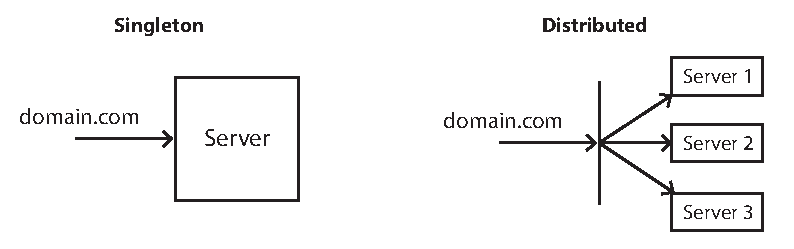
\includegraphics[width=\textwidth]{gfx/server_solutions.pdf}
    \caption{Illustration of a singleton and distributed server solution.}
    \label{fig:server_solutions}
\end{figure}

Distributed server solutions contain several servers possibly on several locations, meaning that DoS will be harder to perform, since there is no single point of failure.
However, this solution cannot ensure consistency and adds complexity.
The two solutions are graphically displayed in Figure~\ref{fig:server_solutions}.
A singleton solution has been chosen due to; consistency and simplicity.
This singleton solution will be denoted as Master or \deno{M}.

The application is required to handle communication with drones, as defined by \at{1} in Figure~\ref{tab:acceptance_tests1}.
In case of the communication being disabled, this might end up with a drone crash.
The technical limitations of antennas for digital wireless communication, sets a constraint for the availability of drones.
Assuming there exists no antenna to cover the physical area of our problem domain, it is necessary to have a distributed antenna setup in order to cover the whole physical area of the problem domain.
This leads to the structure shown in Figure~\ref{fig:antenna_structure}.

\begin{figure}[htb]
    \centering
    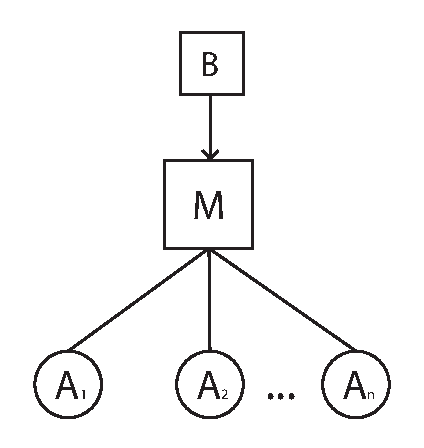
\includegraphics[width=0.5\textwidth]{gfx/antenna_structure.pdf}
    \caption{Antenna structure.}
    \label{fig:antenna_structure}
\end{figure}

If all \deno{B}'s communication with the drones goes through \deno{M}, this would create a single point of failure.
This means that, if \deno{M} crashes at any point, all communication with the drones will be disabled.
Providing the antennas with processing power and opportunity to communicate directly with \deno{B} would solve this issue.
If an antenna crashes only the drones connected to that antenna would be disconnected, leaving the drones connected to other antennas untouched.
This could be achieved by distributing some of the communication from \deno{M}.
This is solved by combining the antennas with distributed processing units, which will be denoted as Slaves or \deno{S}, as shown in Figure~\ref{fig:slave_structure}.

As \deno{S} has a dynamic network position relative to \deno{M}, this enforces that \deno{B} is not able to communicate directly with \deno{S} before getting network information about \deno{S} from \deno{M}. This communication is illustrated by a dashed line in Figure~\ref{fig:slave_structure}.

\begin{figure}[htb]
    \centering
    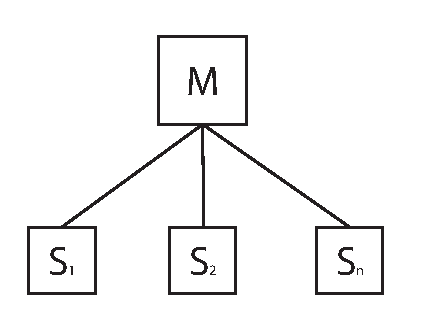
\includegraphics[width=0.5\textwidth]{gfx/slave_structure.pdf}
    \caption{Slave structure.}
    \label{fig:slave_structure}
\end{figure}

The acceptance tests, e.g. 17, 24, 25 in Figure~\ref{tab:acceptance_tests2}, enforces a constraint that requires \deno{M} to be able to store data based of the interaction of the user.
As requests can happen asynchronously, this makes it ideal to use a database denoted \deno{DB}, due to its transaction system in order to ensure no data loss.

The response output of \deno{M} needs to be dynamic based on the user, e.g. Acceptance test 2 in Figure~\ref{tab:acceptance_tests1}, which requires \deno{M} to be capable of processing data and store it in the database.
The processing unit that creates the dynamic response will be denoted \deno{W}.
The communication with the drones are handled by another processing unit, denoted \deno{D}.
If \deno{W} were to handle requests from \deno{S} and \deno{B}, this would increase the load on \deno{W}.
By creating multiple request handlers, it is possible to have a process for each. \deno{W}, \deno{DB}, and \deno{S} are processes, seen in Figure~\ref{fig:daemon_structure}, which improves resource management.
The resource management could be to constrain processing power for each process, or distribute the processes on individual machines.

\begin{figure}[htb]
    \centering
    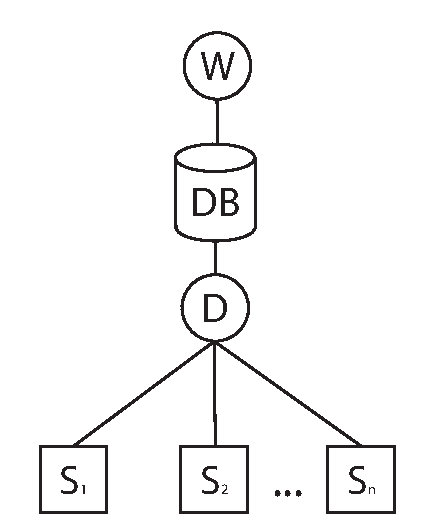
\includegraphics[width=0.5\textwidth]{gfx/daemon_structure.pdf}
    \caption{Daemon structure.}
    \label{fig:daemon_structure}
\end{figure}

% The architecture of \projectname{} differs from other web applications due to the fact that there exists two different type of servers.
% The architecture can be seen in figure~\ref{fig:system_architecture}.
% The server where the web application is running is called Master denoted M.
% For each drone in the system there is a Slave denoted S.
% On both M and S there exists daemons which is responsible for different tasks, however there is some similarity in the tasks they perform.
% These tasks can happen at anytime therefore the program needs to be running at anytime. These daemons are denoted D.
% Each user have a browser they view the application through this is denoted B.
% It is M's responsibility to communicate with every S in the system.
% S is responsible for all communication with the drone it is parred with.

% When a user wants to interact with a drone in the system a session key is needed.
% Such a session key is generated by S and then given to B through M.
% When both B and S have the same session key it is possible for them to communicate without M.
% This ensures that M does not become a bottleneck for controlling and streaming from drones and it reduces latency.
% When a new drone is added it is controlled by its S. This ensures that the system can scaled out and not have to scale up.
% Scale out means using more than one server where scale up means adding more processors, ram etc. to the server so it can handle more by itself.
% M does not handle commands and streaming, and every drone in the system have their own S.
% This makes the application architecture scalable because it removes bottlenecks from both M and S's.

% \begin{figure}[htb]
%     \centering
%     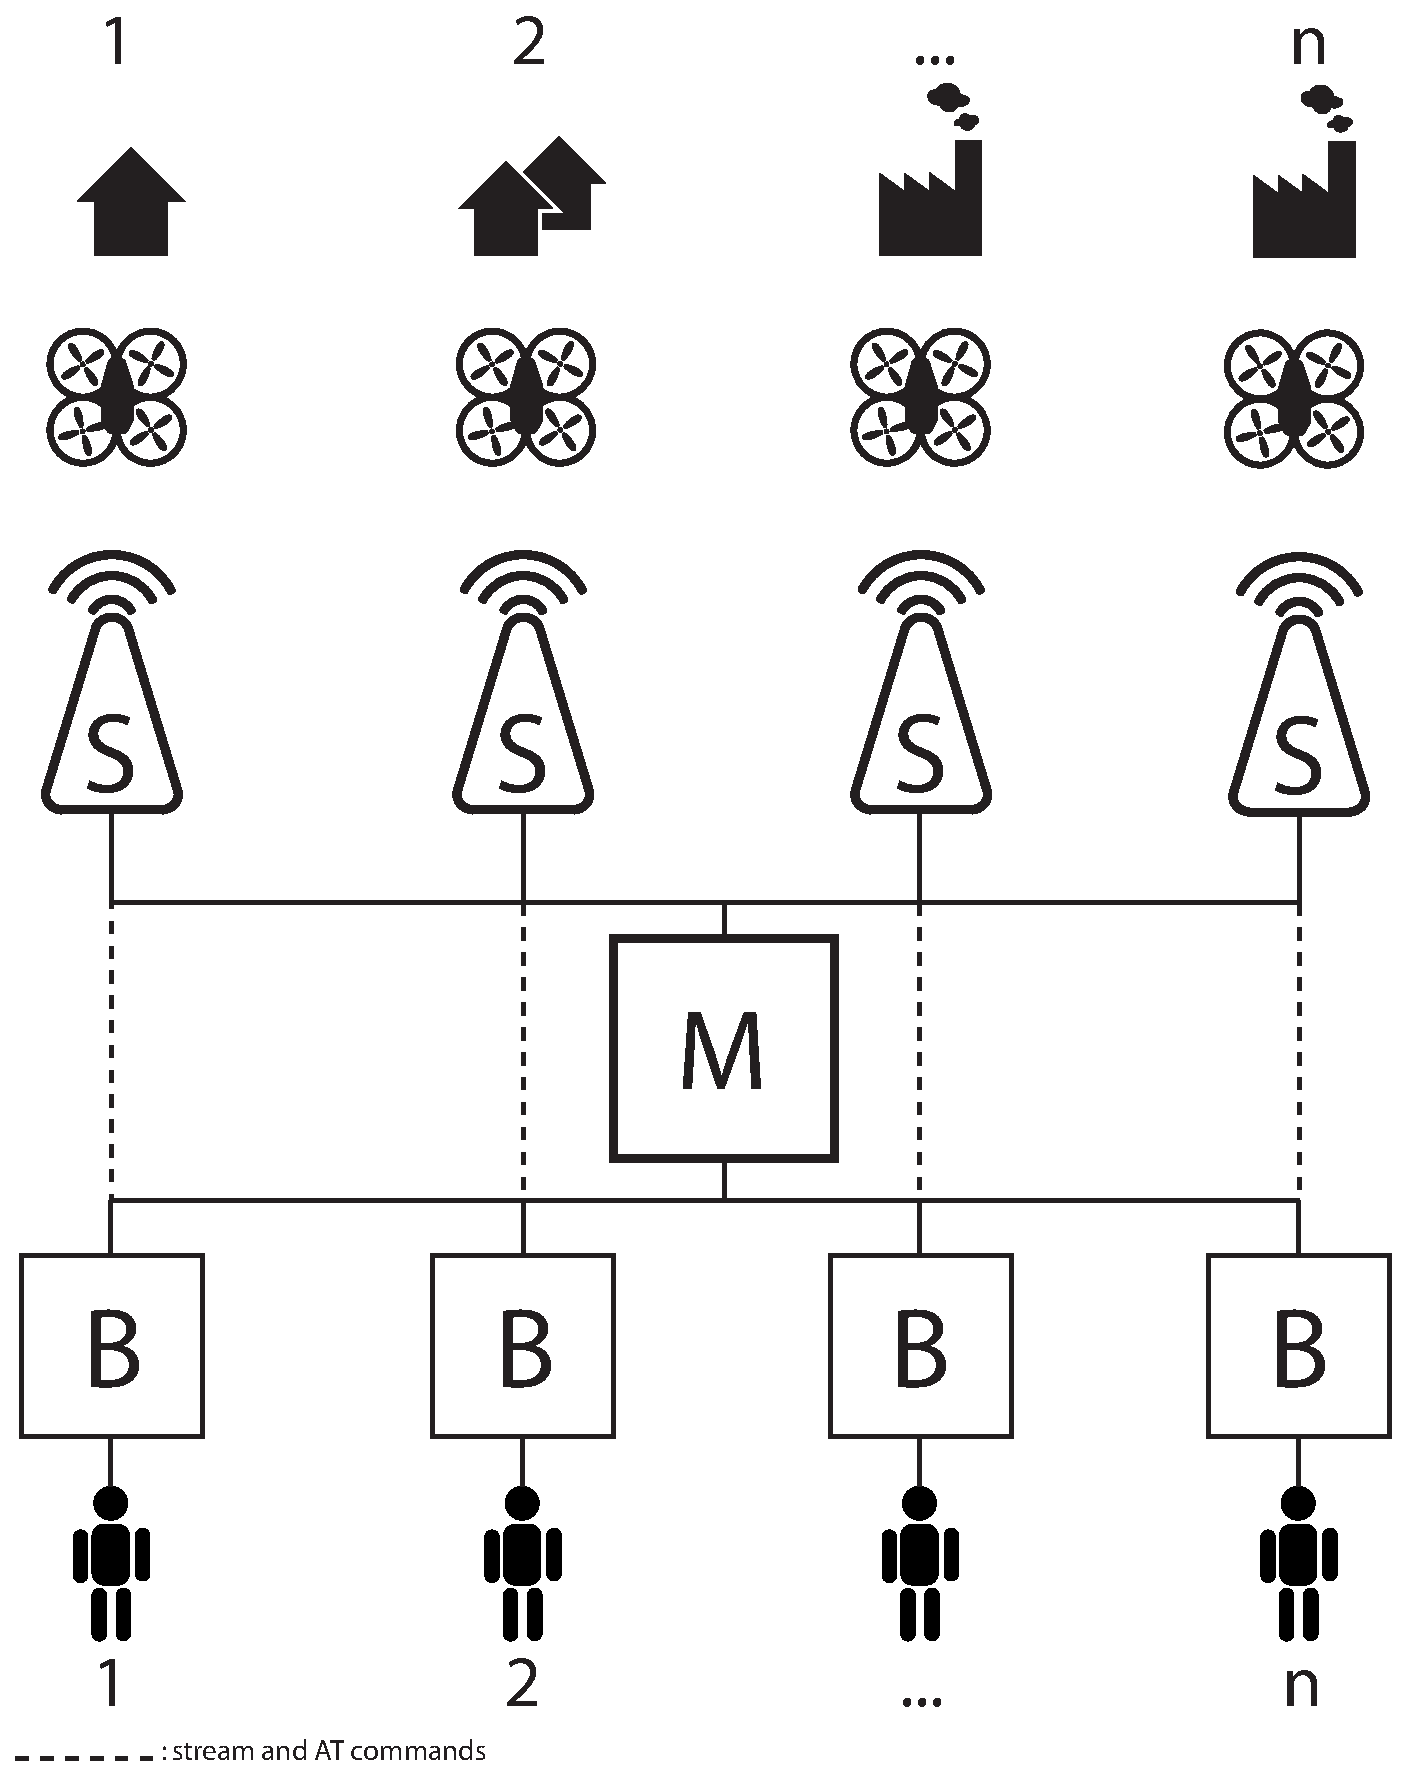
\includegraphics[width=\textwidth]{gfx/system_architecture.pdf}
%     \caption{System architecture of \projectname{}}
%     \label{fig:system_architecture}
% \end{figure}

% The system only uses one M. This can also be seen the bottleneck of the system.
% If M crashes all S's and B's will have to wait for M to come back up.
% One alternative could be running with more M's and in that way scale out.

% There is always one S for each drone connected to the system.
% In this way the system is scaled out.
% This ensures that any S is not likely to become a bottleneck.
% This was done because the drone uses wireless network which is short ranged and the drone is the host which means that the server needs one wireless connection for each drone it have to transmit to.
% One alternative could be only running with one S at each company and just scale it up.
% The problem with this is the server will need a wireless connection for each drone it have to control and it have to be in range.

% Daemon is a background process on a Linux system.
% Daemons are used when it is needed that a process is running at all times.
% In \projectname{} there are both the session key system which both resides on M and S and a policy file system for Adobe Flash on S.
% Both of these processes needs to be running at all times for the user to interact with the drone on S.
\section{Functionality distribution}\label{sec:functionality_distrubution}
% Hvilke funktionaliteter skal dækkes?
% Hvilke instancer dækker hvad?
% Hvorfor gør de det?

The functionality of the system can be derived from the acceptance tests.
This section will cover what instances are responsible for each functionality.

The need for storing data is derived from \at{1}, as previously described this is handled by the database \deno{DB}, which is a part of \deno{M}.
\at{2} sets the need for a dynamic response to \deno{B}, which requires processing of the stored data.
This processing is handled by Web or \deno{W} as the structure contains a singleton server solution.

Knowing that \deno{S} has a dynamic location relative to \deno{M}, this requires \deno{S} to send a signal to the daemon or \deno{D} in order for \deno{M} to get the location of \deno{S} on the network.
\deno{D} is then responsible for being able to receive incoming signals from \deno{S}.

Displaying video is required of \deno{B} by \at{3}.
The video displayed by \deno{B} is a stream, which requires that \deno{S} sends out a video stream.
In order to control a drone, commands have to be provided to the drone, as required by \at{3}.
\deno{S} is responsible for being able to receive commands and have the drone execute the given command.
\at{29} enforces security of the command handler.
\deno{S} is the only instance with a direct link to the drone, this makes \deno{S} responsible for the command handler's security.

% While Section~\ref{sec:application_structure} covered the overall structure of this application, this section will cover how the functionality is divided between the Master and the Slaves in the system. \\

% The Master is the users only way into the system.
% This access will always be via the users local web browser, where he sees the web system for \projectname{}.
% This web system and the database containing all informations about the system, drones, users etc. will be located on the Master.
% The Master is responsible for providing these services and coordinating the communication between the users and drones via the Slaves. \\

% A Slave is needed for every drone in the field, as the drones are not capable of long-distance communication.
% Therefore, in order to communicate with any drone, the communication must be channeled through its assigned Slave.
% This Slave is responsible for keeping contact with the drone and communicate directly with it via its API's.



\section{Communication network}\label{sec:communication_network}

Having functionality distributed across several instances sets the need for communication between the instances.
Based on Figure~\ref{fig:slave_structure}, which displays the dependency between \deno{B}, \deno{M}, and \deno{S} this leads to the diagram shown in Figure~\ref{fig:dataflow_diagrem}. \\


\begin{figure}[!h]
    \centering 
    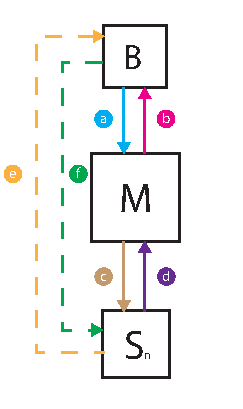
\includegraphics[width=0.5\textwidth]{gfx/dataflow_diagram.pdf}
    \caption{Dataflow diagram of \projectname{}}
    \label{fig:dataflow_diagrem}
\end{figure}


The arrows represent a connection, each connection represent dataflow in the direction of the arrow.
The type of data flowing in each connection and the reasons behind will be covered as each connection is discussed below. \\

Connection \deno{a} covers requests made by \deno{B}, which covers HTTP requests, which is a limit of web solutions that they must use the HTTP protocol.
HTTP requests enable the user to view the web application through his browser, and to send information.
In order to fulfill the request created by \deno{a}, a response is needed which the connection \deno{b} handles.
This connection covers the flow of the dynamic content created by \deno{M}, and static content such as: images, stylesheets, and multimedia objects.
Connection \deno{b} sends both the static and dynamic content back to \deno{B} to be displayed for the user. \\

The connection \deno{d} handles the signal described in Section~\ref{sec:functionality_distribution}.
This signal covers the initial communication between \deno{S} and \deno{M}. \deno{M} verifies the identity of \deno{S} by \deno{S} sending its own unique identifier.
This unique identifier is a string, which consist of X characters \fixme{How many chars?}.
All unique identifiers of each \deno{S} is known to \deno{M}.
This allows \deno{M} to determine the identity of each incoming signal. When \deno{M} receives a signal, and verify the identity of \deno{S}, the source location of the signal is stored in \deno{M} making \deno{M} able to know the location of \deno{S}. \\

Since requests from \deno{B} can happen asynchronously and from dynamic locations, it can create a problem that the identity of the connection made from \deno{S} to \deno{f} is not known. 
\at{28} sets the requirement of differentiating between incoming connections to \deno{S}.
If the communication described in connection \deno{e} and connection \deno{f} were running through \deno{M}, this would be no problem as security would be handled by the already existing sessions on \deno{M}.
The connections \deno{e} and \deno{f} are required to transport a large amount of data.
This data covers a video feed of the drone's video camera and commands for the drone.
This would increase the load on \deno{M}, which is not desired as \deno{M} is assumed to have a high load already.
However, since connection \deno{e} and connection \deno{f} are not running through \deno{M}, this leaves the problem of which \deno{B}, \deno{S} should listen to. \\

The solution chosen to solve this problem is to make \deno{S} create a randomly generated key (session key), that contains 40 characters and is unique relative to \deno{S} stored on \deno{S} itself.
When \deno{S} receives incoming commands, \deno{S} verifies whether or not the key received along with the command is equal to the one locally stored on \deno{S}.
If this is the case, \deno{S} classifies the received command as valid and performs the action.
The session key is delivered to \deno{B} from \deno{M}, as \deno{M} is able to verify the identity of \deno{B} through the session. \\

The connection \deno{c} covers requesting a session key by \deno{M}.
As \deno{M} has a static location, \deno{S} is able to verify the identity of \deno{M} based on its location.
Connection \deno{d} covers the response of the request received in \deno{c}, and \deno{M} is able to verify the identity of \deno{S} based on its location. \\

\begin{figure}[!h]
    \centering 
    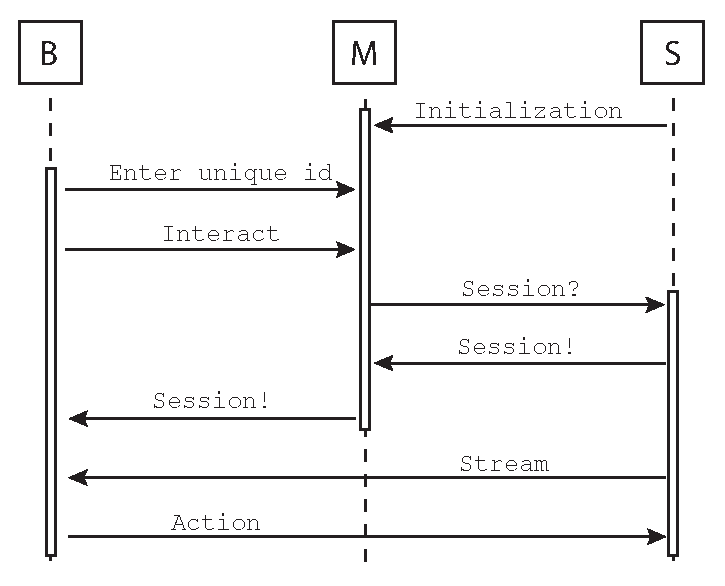
\includegraphics[width=\textwidth]{gfx/sequence_diagram.pdf}
    \caption{Sequence diagram of the communication network between \deno{B}, \deno{M}, and \deno{S}}
    \label{fig:sequence_diagram}
\end{figure}
\fxfatal{Check UML notation.}


The functionalities of the described connections, can only happen in a sequence as illustrated in Figure~\ref{fig:sequence_diagram}.
Each message in the sequence diagram can be done multiple times, however above messages are enforced to be performed atleast once in order for the given message to be performed. \\


% The communication network is crucial for \projectname{} to work.
% When designing a scalable communication network it is important to choose the right structure.
% There are different ways when designing such a network but identical for them all is that they need to support the structure of \deno{M}, \deno{S} and \deno{B} described in section~\ref{sec:application_structure}.

% One solution is to make a structure where \deno{M}, \deno{S} and \deno{B} talk to each other with a level of security. 
% The security aspect would be implemented with a form of session key. 
% This key would be used to determine if a session between a \deno{B} and a \deno{S} is valid.
% Another solution is to provide no security aspect and let it be up to the users and / or company to keep drones safe from intruders.
% This would lessen the communication between \deno{B}, \deno{M} and \deno{S}.  
% It would also decrease the load on \deno{M} and \deno{S}'s database. 
% On the down side the system could be considered not safe because it would be possible to tamper with the drones.
% As this is a system where it is important that the integrity is high, evidence is not tampered with, and where the outcome of an unauthorized user controller a drone could be devastating, it is important to deliver some form of security.



% This lead to a solution where sessions is designed to keep the integrity and secure evidence as seen in figure~\ref{fig:sequence_diagram}. 
% As seen in the figure there is designed a level of security because of the sessions.
% It is not possible for a \deno{B} to interact with a drone without having a session with a drones \deno{S}.

% When a drone is purchased a \deno{S} is setup at the location where the drone is going to operate.
% The \deno{S} sends an initializing message to \deno{M}, informing \deno{M} that a new drone has entered the system.
% \deno{M} adds the drone with the IP and location of the \deno{S}, along with the drone's unique identifier.
% If \deno{M} receives an initializing message from a \deno{S} with a drone identifier that is already in the system, it will destroy any session that correlates with that drone.
% The sessions is destroyed because if one or more sessions are granted and \deno{S} sends its initializing message it is safe to assume that \deno{S} either disconnected or crashed and all sessions keys are invalid.
% Furthermore if the IP of \deno{S} differs from the IP \deno{M} holds in its database it will be updated.

% If a user tries to interact with a drone the system behaves differently.
% A session key will be made on a \deno{S}, this key will be send to \deno{M} and giving to \deno{B}. If this session key is valid it is possible for the user to communicate directly with \deno{S} without \deno{M}.

% \begin{figure}[!h]
%     \centering 
%     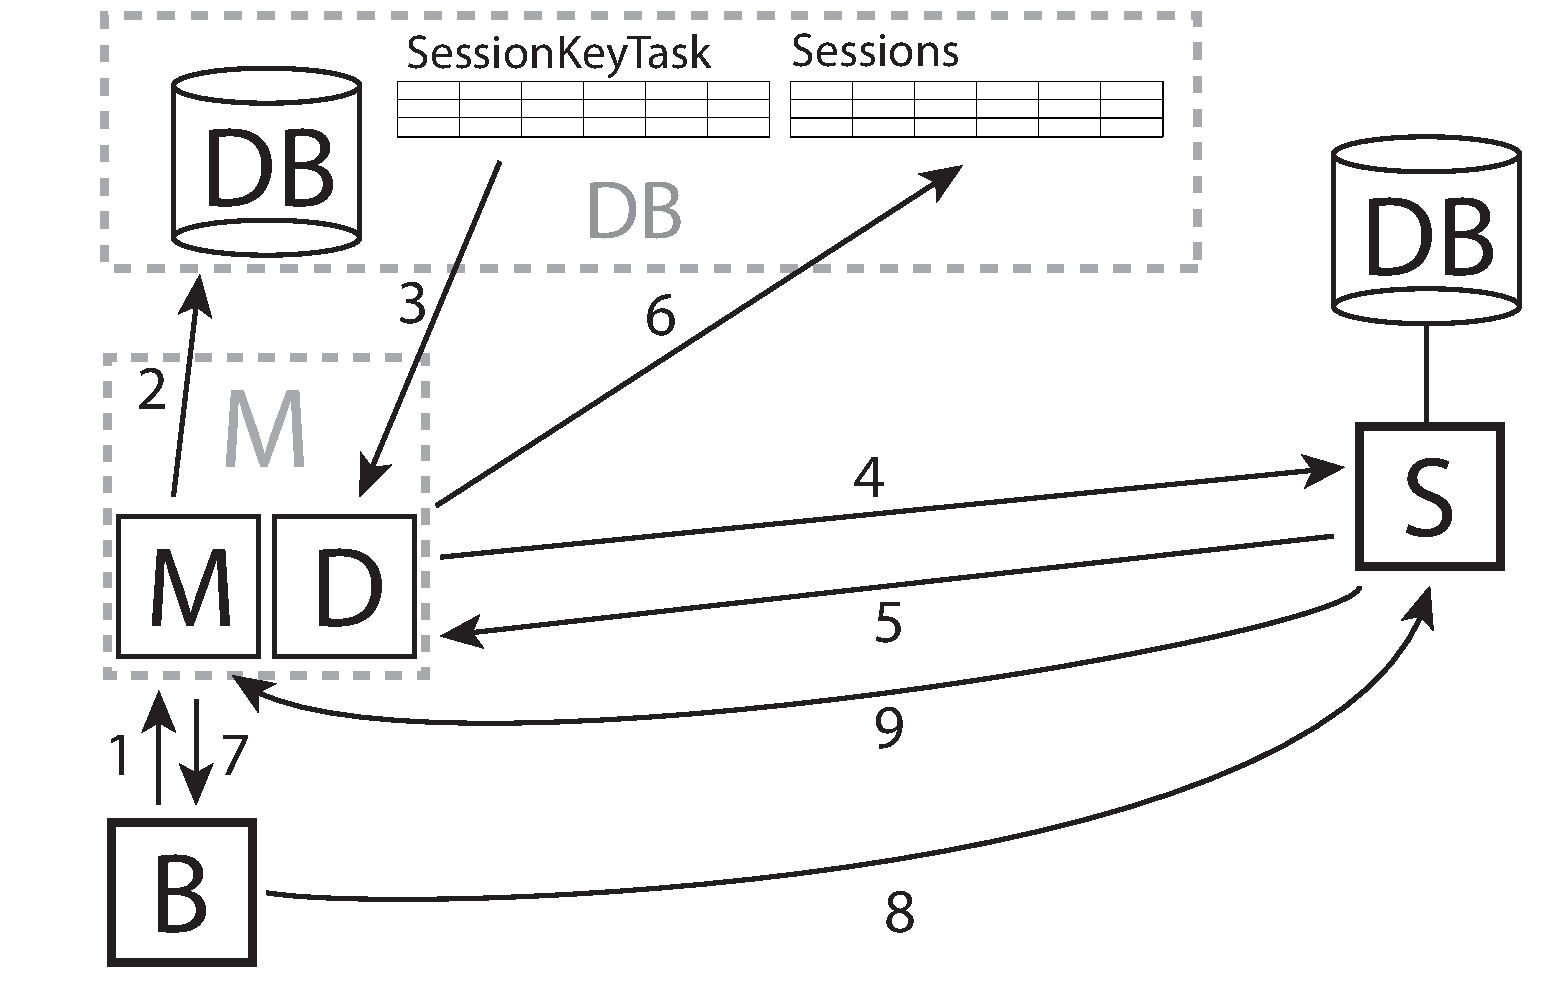
\includegraphics[width=\textwidth]{gfx/sessionkey_communication.pdf}
%     \caption{Session key communication between \deno{B}, \deno{M}, and \deno{S}}
%     \label{fig:sessionkey_communication}
% \end{figure}

% This behavior can be seen in figure~\ref{fig:sessionkey_communication}. 

% Session keys have been designed for security reasons.
% Firstly they were designed to ensure that only one user at a time can control a drone.
% Secondly it ensured that unauthorized users do not have the possibility of controlling a drone.

% \begin{enumerate}
% 	\item Request send from \deno{B} to \deno{M} about getting a session key to interact with a drone.
% 	\item \deno{M} inserts this request in its database table called SessionKeyTask.
% 	\item \deno{D} scans the database table SessionKeyTask, when it sees a new entry it select it and then deletes it from the table.
% 	\item \deno{D} requests a session key from \deno{S} parred with the drone the user wants to interact with.
% 	\item \deno{S} makes a random generated string with uppercase, lowercase letters and number. This string is used as the session key. \deno{S} updates its database with this session key and then sends it back to \deno{D} on \deno{M}.
% 	\item \deno{D} inserts the newly received session key into the session table of \deno{M}.
% 	\item \deno{M} then contacts \deno{B} with the session key.
% 	\item \deno{B} uses this session key to access \deno{S} and through it interact with the drone.
% 	\item A Timeout happens if \deno{B} and \deno{S} does not communicate for 10 seconds.
% \end{enumerate}

% Communication between the servers in the system is crucial. 
% Therefore it is important design a method or a set of methods handling the communication between them. 
% One method could be to make a service which handles all these requests on each server.
% The problem however is that using a single service might create a bottleneck.
% An alternative solution is to make a service for each communication level.
% One service that handles sessions, a service that handles control commands, and a service that handles initial messages from \deno{S} see section~\ref{sec:application_structure}.\fxfatal{Den her paragraf er uspecifik}

% This lead to a solution where the different actors in the system delivered and / or depended on services.

% The interface of the communication network can be seen in figure~\ref{fig:communication_network}.

% The communication network of \projectname{} uses four different ports for providing its services:

% \begin{itemize}
% 	\item Port A - service port for sending and receiving drone control commands.
% 	\item Port B - service port for receiving and sending initial messages.
% 	\item Port C - service port for sending and receiving session information including session keys.
% 	\item Port Web - service port for sending and receiving web specific information.
% \end{itemize}

% \begin{figure}[!h]
%     \centering 
%     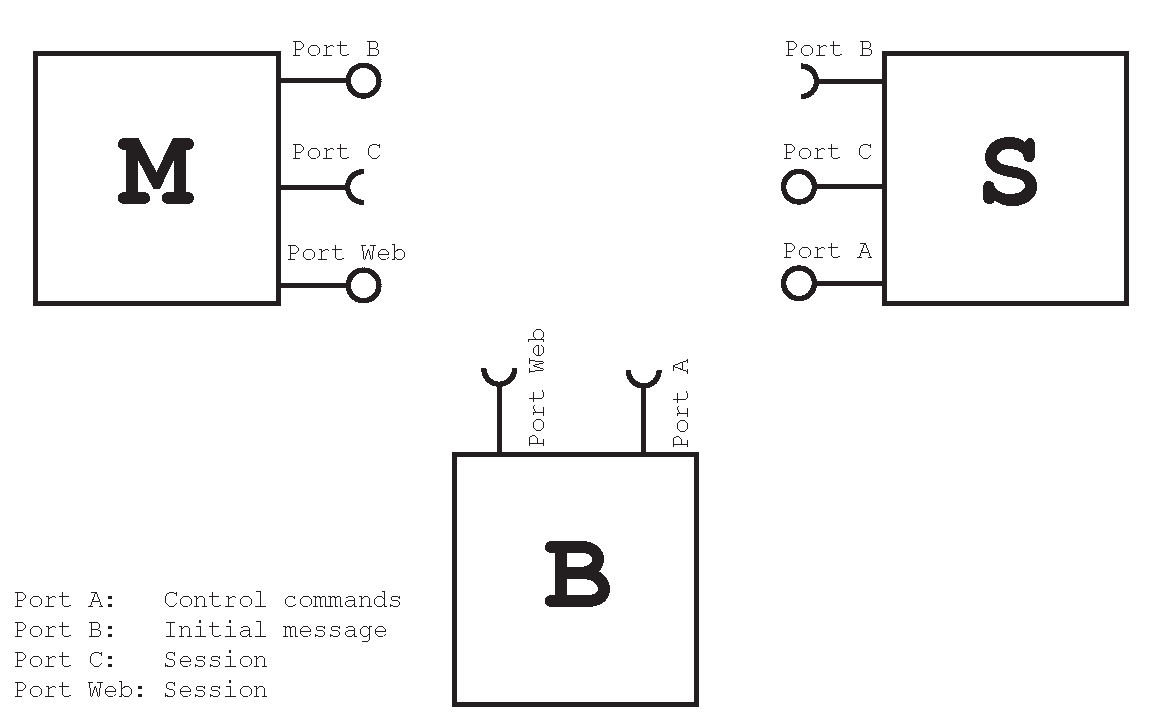
\includegraphics[width=\textwidth]{gfx/communication_network.pdf}
%     \caption{Communication network between \deno{B}, \deno{M}, and \deno{S}}
%     \label{fig:communication_network}
% \end{figure}

% When designing a communication network it is also important to select the right technique for exchanging data between services.
% One of the more widely used techniques are Extensible Markup Language.
% Extensible Markup Language, or XML for short, is a markup language designed to easily mark up data.
% The markup that XML provides makes it possible to easily send and receive data.
% The Extensible in XML makes it possible to extent what data types XML can handle through the XML schema. \citep{simonstl}
% This gives XML a drawback because XML is designed to be extensible it also carries a lot of overhead when used to mark up data.

% \projectname{} needs to be scalable therefore it is important to use as little overhead when sending structured information.
% Otherwise there is a chance that this overhead creates a bottleneck within the network.

% JSON, or JavaScript Object Notation, is design for data interchange and to be human-readable.
% It have a simpler syntax than XML and is not build to be extensible, it is not even a markup language. 
% It is a structured way of exchanging data between sources. 
% This results in less overhead i.e. it costs less data for each piece of information. 
% JSON is also data orientated which makes it easier to map a JSON object directly to a object orientated structure.
% Douglas Crockford call JSON ``The Fat-Free Alternative to XML'' \citep{JSON}.

% Therefore JSON is the perfect format for data interchange between the different services in \projectname{}. There are lesser costs associated with JSON than XML and it is easier to map them into a object orientated language.
\section{Object Model}
\label{section:uml_notation}
\label{subsec:objects}

This section will cover the design choices behind the application's object model, derived from the use cases in Section~\ref{sec:use_cases}.
The UML object model diagram can be seen in Figure~\ref{fig:UML_class_diagram}, and is guided by the UML standard guide written in cooperation by several different software companies~\citep{UML_notation}.\\

The UML attribute notation in this report is:
\begin{itemize}
    \item PK attribute - means that the attribute is a primary key.
    \item FK attribute - means that the attribute is a foreign key.
    \item attribute : type - all attributes will have a type e.g. \verb+id : int+.
\end{itemize}

The system will contain the following objects: \deno{Affiliate Privilege}, \deno{Company}, \deno{Drone}, \deno{Privilege}, \deno{Role}, \deno{Session}, and \deno{User}.
The model of the objects and their relationships can be seen in Figure~\ref{fig:UML_class_diagram}.
Each object covered is represented in the object model diagram with its name in lowercase and pluralized, e.g. \deno{User} object $\rightarrow$ \deno{users}.
If an object's name consists of several words the spaces will be replaced by underscores, e.g. Session Key Task becomes session\_key\_tasks.
The relationships between objects can either be implicit with a line directly from one object to another, or explicit with a simple or rich relationship model between the two objects.
Simple relationship models are models without a PK.
They are represented in the model diagram with both objects in lowercase and pluralized, e.g. roles\_users.
Rich relationship models have a PK.
This kind of relationship model does not have a predetermined naming convention, therefore it can be anything as long as it does not collide with the other model names, e.g. user\_privileges.\\

\begin{figure}[htb]
    \centering
    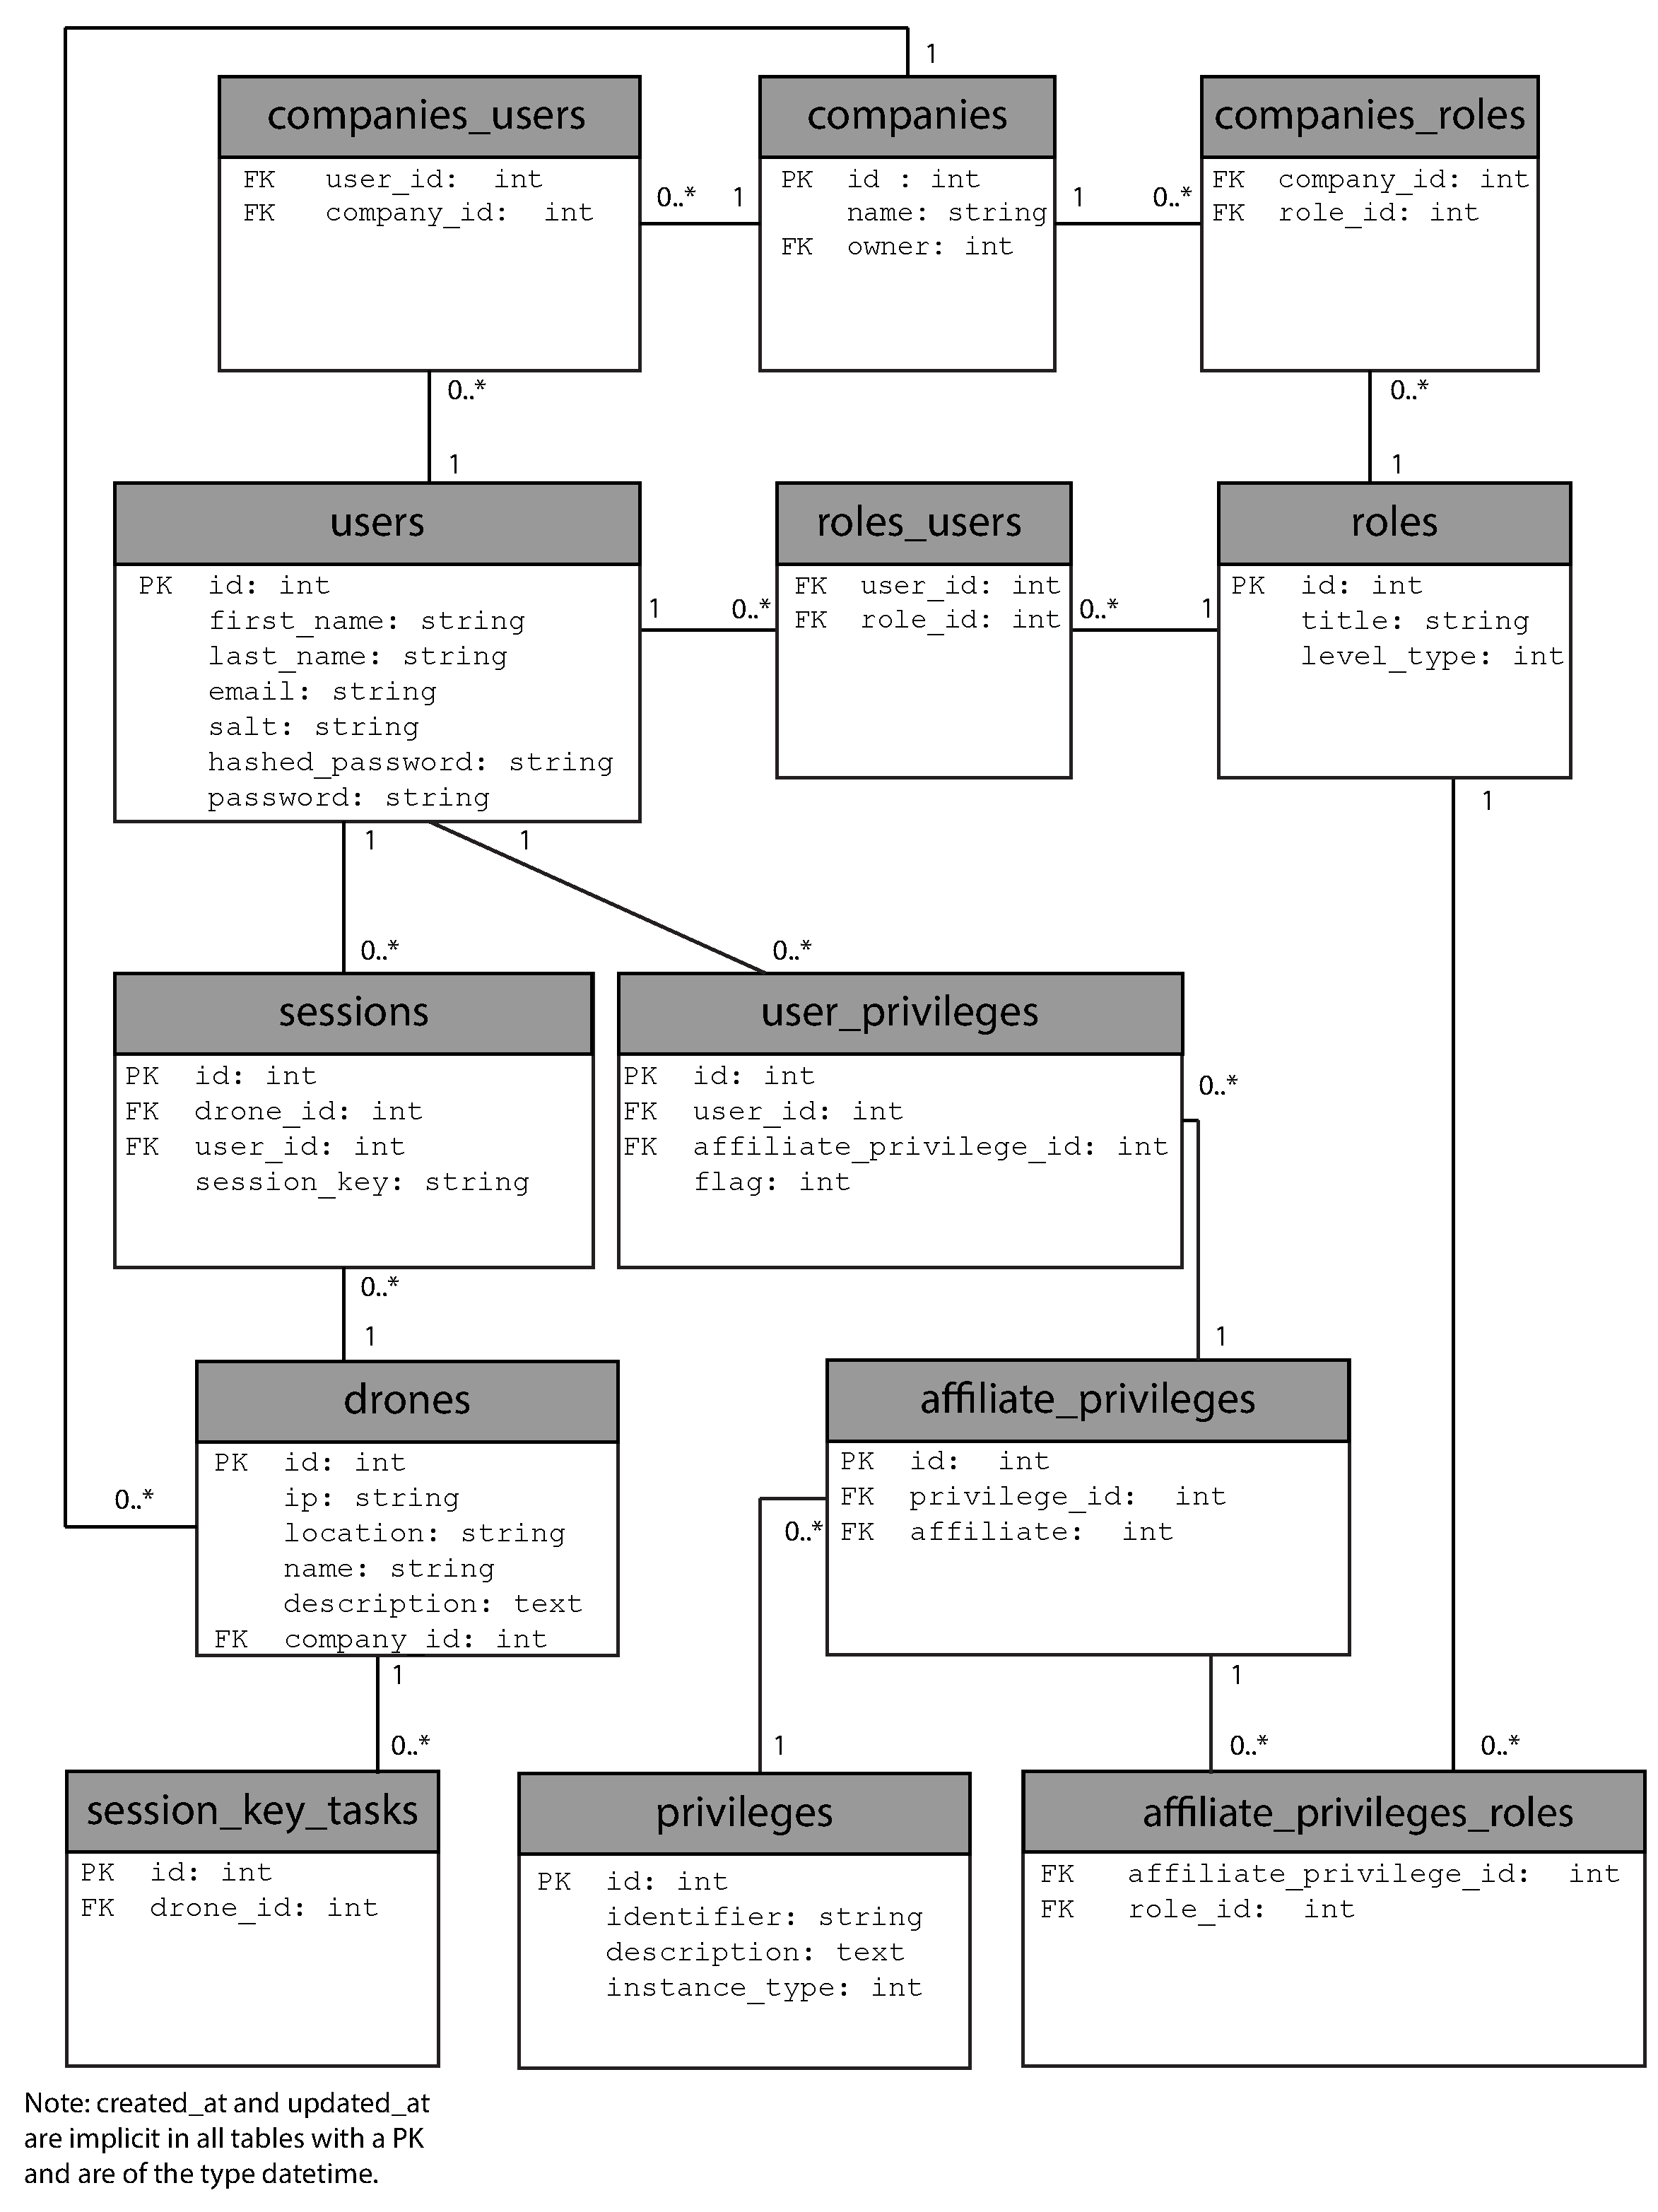
\includegraphics[width=0.95\textwidth]{gfx/UML_model.pdf}
    \caption{UML Class Diagram of \projectname{}}
    \label{fig:UML_class_diagram}
\end{figure}


\subsection{Objects}\fixme{Skal denne overskrift være der? Det burde ikke være nødvendigt at have den, men så skal teksten ændres lidt.}
Access to and actions of the system is restricted.
This restriction is based on the identity of user in the system.
An instance of the \deno{User} object represents a user to the system.
The \deno{User} object has the attributes \verb+email+ and \verb+password+, as seen in Figure~\ref{tab:user_object} in Appendix~\ref{app:objects}, these combined form the login credentials needed for a user to authenticate his identity towards the system. \\

The \verb+email+ is publicly available, which leaves the \verb+password+ to be protected in order for user to protect his identity in the system.
The \verb+password+ entered by the user is concatenated with a \verb+salt+ and hashed through a SHA-1 hashing algorithm to be stored in \verb+hashed_password+.
The hashing algorithm provides a way for storing the password without having its exact value, as this could leave to a security flaw.
Having access to passwords of users directly, e.g. through a hacker attack, would allow the hacker to login into the users account, which is unintended for the system.
When a salt is concatenated before hashing it makes it harder for the hacker to gain the original passwords, e.g. through a rainbow table~\cite{something}. \\

Having a distributed setup with multiple \deno{S}, each representing a \deno{Drone} object, means that the network locations of these need to be known in order to communicate.
The network location is stored in the \verb+ip+ field of the \deno{Drone} object, as shown in Figure~\ref{tab:drone_object} of Appendix~\ref{app:objects}.
The physical drone have a unique identifier known as \verb+name+, which makes the user able to identify a given drone. \\

The users of the system will be part of different companies, therefore there is a need for grouping users by a company.
The \deno{Company} object have an \verb+owner+, which is a reference to a \deno{User} object.
This is required for the system to know which user have access to all \deno{Affiliate Privilege} objects of the company. \\

An \deno{Affiliate Privilege} object references a \deno{Privilege}, and only when combined they form a unique key.
This key unlocks a certain functionality, meaning that if the user does not have a relation to the \deno{Affiliate Privilege} object, which represents the key, then the user is not able to unlock that functionality.
\deno{Role} objects give the possibility of grouping \deno{Privilege} objects together.
Each \deno{Company} have a related role which contains all privileges, of which the company have full control.
Full control gives the right for passing on a privilege, or disabling if the privilege is already granted.
\deno{Affiliate Privilege} objects have a field \verb+affiliate+ that links the privilege to an object of the type declared by the referenced \deno{Privilege} object's \verb+instance_type+ field. \\

The \deno{Session} object represents an active pilot connection between a user and a drone.
The \verb+session_key+ field provides a key that needs to be sent along with the commands.
The \deno{Session Key Task} object is an object used for \deno{D} and \deno{M} to communicate through \deno{DB}, as shown in Figure~\ref{fig:daemon_structure} in Section~\ref{sec:application_structure}. \\

In Section~\ref{sec:privileges} solutions for handling privileges were discussed.
From this discussion it was decided to model a system capable of handling all proposed solutions to fit scenarios of the users.
The \deno{User Privileges} relationship allows for connecting individual {Privilege} objects to a \deno{User} object.
This is could be either granting or revoking, i.e. exceptions, the privilege.
The \verb+flag+ field represents a value of either 1 or -1; 1 is regarded as granted, and -1 is regarded as revoked.


% \subsection{Relationships}
% The system is designed with flexibility and scalability in mind, and the structure of Roles and Privileges are what provides those features.
% As described before there are two ways that a User can be granted a specific Privilege.
% These are by 1) getting the Privilege granted directly via the \verb+User_Privileges+ table or 2) by being a member of a Role that via the \verb+Privileges_Roles+ table that has one or more Privileges granted.
% These will be explained in details in the following subsections.


% % Users and Privileges %
% An administrator can grant a specific Privilege directly to a user via the \verb+User_Privileges+ table.
% This Privilege is then affiliated with an object -- usually a Drone.
% The Privilege could also be a system functionality, however, as described in Section~\ref{sec:privileges}. \\

% This relationship is also used for exceptions.
% In an example where five Users: U1, U2, U3, U4 and U5 are a member of a Role: R1, we may have a situation where U2 is not suppose to have access to a given Privilege P1 in R1.
% Then a User-specific Privilege is granted to U2 on P1, but with the ``exception''-flag marked.
% This is equal to blacklisting U2 from using Privilege P1, providing the system with a lot of flexibility, as even though a group of Users are granted a number of Privileges via a role, User-specific exceptions can be added to this setting. \\


% % Roles and Privileges %
% As mentioned before -- the reason that Roles can be used to assign Privileges to a User, is to make both the administration and data structure of Users and Privileges as simple and efficient as possible.
% By allowing exceptions, full flexibility is still possible. \\

% This is how the relationship between Roles and Privileges works: \\

% An administrator creates a Role.
% Lets call this Role ``Control Drone \#4''.
% A number of Privileges are assigned to this Role.
% It could be the following:

% \begin{itemize}
%     \item Watch the video feed from a specific drone
%     \item Control the movement of a specific drone
% \end{itemize}

% Those Privileges are then linked to this Role and to the Drone this concerns. \\

% Roles can be assigned with affiliation to both Users and Companies.
% Say a user \verb+U1+ needs access to Drone \#4.
% User U1 then needs to either have the Privileges directly granted or be a member of the role ``Control Drone \#4''.


% % Privileges and granting of Privileges %
% Since it is possible to grant Privileges both directly to a User and via a Role, the same Privilege can be used in more than one context.
% Therefore the \verb+Affiliation_Privileges+ table exists.
% This table links the granting of a Privilege with the actual Privilege and defines on which Object the Privilege applies.
% The reason for having this table and not just link the two granting-tables \verb+User_Privileges+ and \verb+Privileges_Roles+ directly to the \verb+Privileges+ table, is that we try to avoid redundant data by having the data in the \verb+Privileges+ and \verb+Affiliation_Privileges+ table make up one instance of a privilege together.
% This is then granted to a User or a Role, who can then use the Privilege. \\

% The system is designed so that any User can grant a Privilege he already has already been granted to another User if he is permitted to.
% This is controlled via a ``re-grantable'' flag which is set in either the \verb+User_Privileges+ table or the \verb+Privileges_Roles+ table.
% By marking this flag as ``true'', the User or Users that via a Role is granted the Privilege in question, can via an interface in the system re-grant the Privilege to other Users in the same Company.


% %Note: Alle brugere kan videregrante et privilege hvis de har tilladelse til det. Det er et flag som sætes i user_privileges og privileges_roles, som tillader alle der har dette privilegie til at videregrante det. Husk at beskrive hvordan et privilege og et affiliation privilege til sammen giver et grant-able privilegie


% % Privileges and Drones %
% With \projectname{} in its current form, most Privileges that are granted will have an connected with a Drone.
% Privileges and its a affiliations are linked in the \verb+Affiliation_Privileges+ table.
% This is also where Drones are linked to any granted privilege. \\

% As described earlier, Drones are the current object-type implemented in the system.
% However, the structure and model of the system allows for later expansion, connection new objects such as stationary cameras or any other type of object to the system.
% The \verb+Affiliation_Privileges+ has a third field named \verb+object_id+.
% This field links the Privilege, the granting of it and the Object that this granting is valid for. \\

% An example could be linking Privilege P1, User U1 and Drone D1.
% Say P1 is the privilege for watching the video feed of a drone.
% Then the user U1 will have access to watch the video feed of Drone D1.


% % Drones and Companies %
% The \verb+Company_drones+ table defines a relationship between a Drone and a Company.

% The administrator of each Company defines the Roles in that Company.
% In doing so, he defines which Privileges that are granted in every Role.
% These Privileges are linked to a (Drone)-object.
% The system must make sure that any Company administrator cannot link a Privilege with a Object that is not within his control. \\

% This relationship defines which Drones are available to each Company.
% When a Company administrator adds new Roles (and hence Privileges), he is only able to associate it with Drones that are connected to the Company in question.

% **************************************************************************************************************
% A Classic Thesis Style
% An Homage to The Elements of Typographic Style
%
% Copyright (C) 2012 Andr\'e Miede http://www.miede.de
%
% If you like the style then I would appreciate a postcard. My address
% can be found in the file ClassicThesis.pdf. A collection of the
% postcards I received so far is available online at
% http://postcards.miede.de
%
% License:
% This program is free software; you can redistribute it and/or modify
% it under the terms of the GNU General Public License as published by
% the Free Software Foundation; either version 2 of the License, or
% (at your option) any later version.
%
% This program is distributed in the hope that it will be useful,
% but WITHOUT ANY WARRANTY; without even the implied warranty of
% MERCHANTABILITY or FITNESS FOR A PARTICULAR PURPOSE.  See the
% GNU General Public License for more details.
%
% You should have received a copy of the GNU General Public License
% along with this program; see the file COPYING.  If not, write to
% the Free Software Foundation, Inc., 59 Temple Place - Suite 330,
% Boston, MA 02111-1307, USA.
%
% **************************************************************************************************************
% Note:
%    * You must not use "u etc. in strings/commands that will be spaced out (use \"u or real umlauts instead)
%    * New enumeration (small caps): \begin{aenumerate} \end{aenumerate}
%    * For margin notes: \marginpar or \graffito{}
%    * Do not use bold fonts in this style, it is designed around them
%    * Use tables as in the examples
%    * See classicthesis-preamble.sty for useful commands
% **************************************************************************************************************
% To Do:
%		 * [high] Check this out: http://www.golatex.de/koma-script-warnung-in-verbindung-mit-listings-package-t2058.html
%    * [medium] mathbb in section-titles/chapter-titles => disappears somehow in headlines!!!
% **************************************************************************************************************
\documentclass[ twoside,openright,titlepage,numbers=noenddot,headinclude,%1headlines,% letterpaper a4paper
                footinclude=true,cleardoublepage=empty,abstractoff, % <--- obsolete, remove (todo)
                BCOR=5mm,paper=a4,fontsize=11pt,%11pt,a4paper,%
                ngerman,american,%
                ]{scrreprt}

%********************************************************************
% Note: Make all your adjustments in here
%*******************************************************
% ****************************************************************************************************
% classicthesis-config.tex
% formerly known as loadpackages.sty, classicthesis-ldpkg.sty, and classicthesis-preamble.sty
% Use it at the beginning of your ClassicThesis.tex, or as a LaTeX Preamble
% in your ClassicThesis.{tex,lyx} with \input{classicthesis-config}
% ****************************************************************************************************
% If you like the classicthesis, then I would appreciate a postcard.
% My address can be found in the file ClassicThesis.pdf. A collection
% of the postcards I received so far is available online at
% http://postcards.miede.de
% ****************************************************************************************************

% ****************************************************************************************************
% 1. Configure classicthesis for your needs here, e.g., remove "drafting" below
% in order to deactivate the time-stamp on the pages
% ****************************************************************************************************
\PassOptionsToPackage{eulerchapternumbers,listings,drafting,%
				 pdfspacing,%floatperchapter,%linedheaders,%
				 subfig,beramono,eulermath,parts}{classicthesis}
% ********************************************************************
% Available options for classicthesis.sty
% (see ClassicThesis.pdf for more information):
% drafting
% parts nochapters linedheaders
% eulerchapternumbers beramono eulermath pdfspacing minionprospacing
% tocaligned dottedtoc manychapters
% listings floatperchapter subfig
% ********************************************************************

% ********************************************************************
% Triggers for this config
% ********************************************************************
\usepackage{ifthen}
\newboolean{enable-backrefs} % enable backrefs in the bibliography
\setboolean{enable-backrefs}{false} % true false
% ****************************************************************************************************


% ****************************************************************************************************
% 2. Personal data and user ad-hoc commands
% ****************************************************************************************************
\newcommand{\myTitle}{LONE\xspace}
\newcommand{\mySubtitle}{Lone is Observation of Nondeterministic Environments\xspace}
%\newcommand{\myDegree}{Doktor-Ingenieur (Dr.-Ing.)\xspace}
\newcommand{\myName}{SW701E12\xspace}
\newcommand{\myProf}{Put name here\xspace}
\newcommand{\myOtherProf}{Put name here\xspace}
\newcommand{\mySupervisor}{Put name here\xspace}
\newcommand{\myFaculty}{Put data here\xspace}
\newcommand{\myDepartment}{Put data here\xspace}
\newcommand{\myUni}{Aalborg University\xspace}
\newcommand{\myLocation}{Aalborg\xspace}
\newcommand{\myTime}{December 2012\xspace}
\newcommand{\myVersion}{version 4.1\xspace}
\newcommand{\projectname}{<projectname>}

% ********************************************************************
% Setup, finetuning, and useful commands
% ********************************************************************
\newcounter{dummy} % necessary for correct hyperlinks (to index, bib, etc.)
\newlength{\abcd} % for ab..z string length calculation
\providecommand{\mLyX}{L\kern-.1667em\lower.25em\hbox{Y}\kern-.125emX\@}
\newcommand{\ie}{i.\,e.}
\newcommand{\Ie}{I.\,e.}
\newcommand{\eg}{e.\,g.}
\newcommand{\Eg}{E.\,g.}
% ****************************************************************************************************


% ****************************************************************************************************
% 3. Loading some handy packages
% ****************************************************************************************************
% ********************************************************************
% Packages with options that might require adjustments
% ********************************************************************
\PassOptionsToPackage{latin9}{inputenc}	% latin9 (ISO-8859-9) = latin1+"Euro sign"
 \usepackage{inputenc}

%\PassOptionsToPackage{ngerman,american}{babel}   % change this to your language(s)
% Spanish languages need extra options in order to work with this template
%\PassOptionsToPackage{spanish,es-lcroman}{babel}
 \usepackage{babel}

\PassOptionsToPackage{square,numbers}{natbib}
 \usepackage{natbib}

\PassOptionsToPackage{fleqn}{amsmath}		% math environments and more by the AMS
 \usepackage{amsmath}

% ********************************************************************
% General useful packages
% ********************************************************************
\PassOptionsToPackage{T1}{fontenc} % T2A for cyrillics
	\usepackage{fontenc}
\usepackage{textcomp} % fix warning with missing font shapes
\usepackage{scrhack} % fix warnings when using KOMA with listings package
\usepackage{xspace} % to get the spacing after macros right
\usepackage{mparhack} % get marginpar right
\usepackage{fixltx2e} % fixes some LaTeX stuff
\PassOptionsToPackage{printonlyused,smaller}{acronym}
	\usepackage{acronym} % nice macros for handling all acronyms in the thesis
%\renewcommand*{\acsfont}[1]{\textssc{#1}} % for MinionPro
\renewcommand{\bflabel}[1]{{#1}\hfill} % fix the list of acronyms
\usepackage[footnote,draft,english,silent,nomargin]{fixme}  % final instead of draft produces errors at
                                                            % compile time
                                                            
%Bjarke HS stuff
\newcommand{\todo}[1]{\fxnote{#1}}
\newcommand{\todoi}[1]{\fxfatal{#1}}
\newcommand{\todoI}[1]{\todoi{#1}}

%Rasmus stuff
\newcommand{\figref}[1]{\figurename~\ref{#1}}

% ****************************************************************************************************


% ****************************************************************************************************
% 4. Setup floats: tables, (sub)figures, and captions
% ****************************************************************************************************
\usepackage{tabularx} % better tables
	\setlength{\extrarowheight}{3pt} % increase table row height
\newcommand{\tableheadline}[1]{\multicolumn{1}{c}{\spacedlowsmallcaps{#1}}}
\newcommand{\myfloatalign}{\centering} % to be used with each float for alignment
\usepackage{caption}
\captionsetup{format=hang,font=small}
\usepackage{subfig}
% ****************************************************************************************************


% ****************************************************************************************************
% 5. Setup code listings
% ****************************************************************************************************
\usepackage{listings}
%\lstset{emph={trueIndex,root},emphstyle=\color{BlueViolet}}%\underbar} % for special keywords
\lstset{language=[LaTeX]Tex,%C++,
    keywordstyle=\color{RoyalBlue},%\bfseries,
    basicstyle=\small\ttfamily,
    %identifierstyle=\color{NavyBlue},
    commentstyle=\color{Green}\ttfamily,
    stringstyle=\rmfamily,
    numbers=none,%left,%
    numberstyle=\scriptsize,%\tiny
    stepnumber=5,
    numbersep=8pt,
    showstringspaces=false,
    breaklines=true,
    frameround=ftff,
    frame=single,
    belowcaptionskip=.75\baselineskip
    %frame=L
}
% ****************************************************************************************************


% ****************************************************************************************************
% 6. PDFLaTeX, hyperreferences and citation backreferences
% ****************************************************************************************************
% ********************************************************************
% Using PDFLaTeX
% ********************************************************************
\PassOptionsToPackage{pdftex,hyperfootnotes=false,pdfpagelabels}{hyperref}
	\usepackage{hyperref}  % backref linktocpage pagebackref
\pdfcompresslevel=9
\pdfadjustspacing=1
\PassOptionsToPackage{pdftex}{graphicx}
	\usepackage{graphicx}

% ********************************************************************
% Setup the style of the backrefs from the bibliography
% (translate the options to any language you use)
% ********************************************************************
\newcommand{\backrefnotcitedstring}{\relax}%(Not cited.)
\newcommand{\backrefcitedsinglestring}[1]{(Cited on page~#1.)}
\newcommand{\backrefcitedmultistring}[1]{(Cited on pages~#1.)}
\ifthenelse{\boolean{enable-backrefs}}%
{%
		\PassOptionsToPackage{hyperpageref}{backref}
		\usepackage{backref} % to be loaded after hyperref package
		   \renewcommand{\backreftwosep}{ and~} % separate 2 pages
		   \renewcommand{\backreflastsep}{, and~} % separate last of longer list
		   \renewcommand*{\backref}[1]{}  % disable standard
		   \renewcommand*{\backrefalt}[4]{% detailed backref
		      \ifcase #1 %
		         \backrefnotcitedstring%
		      \or%
		         \backrefcitedsinglestring{#2}%
		      \else%
		         \backrefcitedmultistring{#2}%
		      \fi}%
}{\relax}

% ********************************************************************
% Hyperreferences
% ********************************************************************
\hypersetup{%
    %draft,	% = no hyperlinking at all (useful in b/w printouts)
    colorlinks=true, linktocpage=true, pdfstartpage=3, pdfstartview=FitV,%
    % uncomment the following line if you want to have black links (e.g., for printing)
    %colorlinks=false, linktocpage=false, pdfborder={0 0 0}, pdfstartpage=3, pdfstartview=FitV,%
    breaklinks=true, pdfpagemode=UseNone, pageanchor=true, pdfpagemode=UseOutlines,%
    plainpages=false, bookmarksnumbered, bookmarksopen=true, bookmarksopenlevel=1,%
    hypertexnames=true, pdfhighlight=/O,%nesting=true,%frenchlinks,%
    urlcolor=webbrown, linkcolor=RoyalBlue, citecolor=webgreen, %pagecolor=RoyalBlue,%
    %urlcolor=Black, linkcolor=Black, citecolor=Black, %pagecolor=Black,%
    pdftitle={\myTitle},%
    pdfauthor={\textcopyright\ \myName, \myUni, \myFaculty},%
    pdfsubject={},%
    pdfkeywords={},%
    pdfcreator={pdfLaTeX},%
    pdfproducer={LaTeX with hyperref and classicthesis}%
}

% ********************************************************************
% Setup autoreferences
% ********************************************************************
% There are some issues regarding autorefnames
% http://www.ureader.de/msg/136221647.aspx
% http://www.tex.ac.uk/cgi-bin/texfaq2html?label=latexwords
% you have to redefine the makros for the
% language you use, e.g., american, ngerman
% (as chosen when loading babel/AtBeginDocument)
% ********************************************************************
\makeatletter
\@ifpackageloaded{babel}%
    {%
       \addto\extrasamerican{%
					\renewcommand*{\figureautorefname}{Figure}%
					\renewcommand*{\tableautorefname}{Table}%
					\renewcommand*{\partautorefname}{Part}%
					\renewcommand*{\chapterautorefname}{Chapter}%
					\renewcommand*{\sectionautorefname}{Section}%
					\renewcommand*{\subsectionautorefname}{Section}%
					\renewcommand*{\subsubsectionautorefname}{Section}%
				}%
       \addto\extrasngerman{%
					\renewcommand*{\paragraphautorefname}{Absatz}%
					\renewcommand*{\subparagraphautorefname}{Unterabsatz}%
					\renewcommand*{\footnoteautorefname}{Fu\"snote}%
					\renewcommand*{\FancyVerbLineautorefname}{Zeile}%
					\renewcommand*{\theoremautorefname}{Theorem}%
					\renewcommand*{\appendixautorefname}{Anhang}%
					\renewcommand*{\equationautorefname}{Gleichung}%
					\renewcommand*{\itemautorefname}{Punkt}%
				}%
			% Fix to getting autorefs for subfigures right (thanks to Belinda Vogt for changing the definition)
			\providecommand{\subfigureautorefname}{\figureautorefname}%
    }{\relax}
\makeatother


% ****************************************************************************************************
% 7. Last calls before the bar closes
% ****************************************************************************************************
% ********************************************************************
% Development Stuff
% ********************************************************************
\listfiles
%\PassOptionsToPackage{l2tabu,orthodox,abort}{nag}
%	\usepackage{nag}
%\PassOptionsToPackage{warning, all}{onlyamsmath}
%	\usepackage{onlyamsmath}

% ********************************************************************
% Last, but not least...
% ********************************************************************
\usepackage{classicthesis}
% ****************************************************************************************************


% ****************************************************************************************************
% 8. Further adjustments (experimental)
% ****************************************************************************************************
% ********************************************************************
% Changing the text area
% ********************************************************************
%\linespread{1.05} % a bit more for Palatino
%\areaset[current]{312pt}{761pt} % 686 (factor 2.2) + 33 head + 42 head \the\footskip
%\setlength{\marginparwidth}{7em}%
%\setlength{\marginparsep}{2em}%

% ********************************************************************
% Using different fonts
% ********************************************************************
%\usepackage[oldstylenums]{kpfonts} % oldstyle notextcomp
%\usepackage[osf]{libertine}
%\usepackage{hfoldsty} % Computer Modern with osf
%\usepackage[light,condensed,math]{iwona}
%\renewcommand{\sfdefault}{iwona}
%\usepackage{lmodern} % <-- no osf support :-(
%\usepackage[urw-garamond]{mathdesign} <-- no osf support :-(
% ****************************************************************************************************


%********************************************************************
% Hyphenation
%*******************************************************
%\hyphenation{put special hyphenation here}

% ********************************************************************
% GO!GO!GO! MOVE IT!
%*******************************************************
\begin{document}
\frenchspacing
\raggedbottom
\selectlanguage{american} % american ngerman
%\renewcommand*{\bibname}{new name}
%\setbibpreamble{}
\pagenumbering{roman}
\pagestyle{plain}
%********************************************************************
% Frontmatter
%*******************************************************
%%*******************************************************
% Little Dirty Titlepage
%*******************************************************
\thispagestyle{empty}
%\pdfbookmark[1]{Titel}{title}
%*******************************************************
\begin{center}
    \spacedlowsmallcaps{\myName} \\ \medskip                        

    \begingroup
        \color{Maroon}\spacedallcaps{\myTitle}
    \endgroup
\end{center}        

%*******************************************************
% Titlepage
%*******************************************************
\begin{titlepage}
	% if you want the titlepage to be centered, uncomment and fine-tune the line below (KOMA classes environment)
	\begin{addmargin}[-1cm]{-3cm}
    \begin{center}
        \large  

        \hfill

        \vfill

        \begingroup
            \color{Maroon}\spacedallcaps{\myTitle} \\ \bigskip
        \endgroup

        \vfill

        %\myDegree \\
        %\myDepartment \\                            
        %\myFaculty \\
        %\myUni \\ \bigskip

        \myTime\ -- \myVersion

        \vfill                      

    \end{center}  
  \end{addmargin}       
\end{titlepage}   
\thispagestyle{empty}

\hfill

\vfill

\noindent\myName: \textit{\myTitle,} \mySubtitle, %\myDegree, 
\textcopyright\ \myTime

%\bigskip
%
%\noindent\spacedlowsmallcaps{Supervisors}: \\
%\myProf \\
%\myOtherProf \\ 
%\mySupervisor
%
%\medskip
%
%\noindent\spacedlowsmallcaps{Location}: \\
%\myLocation
%
%\medskip
%
%\noindent\spacedlowsmallcaps{Time Frame}: \\
%\myTime

%\cleardoublepage%*******************************************************
% Dedication
%*******************************************************
\thispagestyle{empty}
%\phantomsection 
\refstepcounter{dummy}
\pdfbookmark[1]{Dedication}{Dedication}

\vspace*{3cm}

\begin{center}
    \emph{Ohana} means family. \\
    Family means nobody gets left behind, or forgotten. \\ \medskip
    --- Lilo \& Stitch    
\end{center}

\medskip

\begin{center}
    Dedicated to the loving memory of Rudolf Miede. \\ \smallskip
    1939\,--\,2005
\end{center}
%\cleardoublepage\include{FrontBackmatter/Foreword}
\cleardoublepage%*******************************************************
% Abstract
%*******************************************************
%\renewcommand{\abstractname}{Abstract}
\pdfbookmark[1]{Abstract}{Abstract}
\begingroup
\let\clearpage\relax
\let\cleardoublepage\relax
\let\cleardoublepage\relax

\chapter*{Abstract}
Video surveilance is becoming more and more used around the world.
Governments use it in big cities to prevent criminal activities and terror, while privates use it to surveil their property and have evidence if a crime happens.
The ways that the technology allows us to video surveil today is, however, quite expensive and has its limitations such as the amount of needed hardware to get a sufficient degree of surveilance and the installation costs of this equipment. \\

This paper seeks to take advantage of modern technology to provide a new way of video surveil large areas in a cost-efficient way. 
A proof of concept solution that uses unmanned air-crafts with mounted cameras -- drones -- and a web-interface for user interacting based on a scalable infrastructure is designed and implemented.
The goal is a scalable web-application that allows multiple users to control and view the video stream from such drones to do remote and cost-efficient surveilance of large areas. \\

The system that was developed in this student project is a proof of concept solution that shows that -- with better hardware than what was available in this project -- a product that uses drones to surveil large areas is possible to deploy. 

\endgroup			

\vfill
%\cleardoublepage%*******************************************************
% Publications
%*******************************************************
\pdfbookmark[1]{Publications}{publications}
\chapter*{Publications}
Some ideas and figures have appeared previously in the following publications:

\bigskip

\noindent Put your publications from the thesis here. The packages \texttt{multibib} or \texttt{bibtopic} etc. can be used to handle multiple different bibliographies in your document.
%\cleardoublepage%*******************************************************
% Acknowledgments
%*******************************************************
\pdfbookmark[1]{Acknowledgments}{acknowledgments}

\begin{flushright}{\slshape    
    We have seen that computer programming is an art, \\ 
    because it applies accumulated knowledge to the world, \\ 
    because it requires skill and ingenuity, and especially \\
    because it produces objects of beauty.} \\ \medskip
    --- \defcitealias{knuth:1974}{Donald E. Knuth}\citetalias{knuth:1974} \citep{knuth:1974}
\end{flushright}



\bigskip

\begingroup
\let\clearpage\relax
\let\cleardoublepage\relax
\let\cleardoublepage\relax
\chapter*{Acknowledgments}
Put your acknowledgments here.

Many thanks to everybody who already sent me a postcard!

Regarding the typography and other help, many thanks go to Marco 
Kuhlmann, Philipp Lehman, Lothar Schlesier, Jim Young, Lorenzo 
Pantieri and Enrico Gregorio\footnote{Members of GuIT (Gruppo 
Italiano Utilizzatori di \TeX\ e \LaTeX )}, J\"org Sommer, 
Joachim K\"ostler, Daniel Gottschlag, Denis Aydin, Paride 
Legovini, Steffen Prochnow, Nicolas Repp, Hinrich Harms, 
 Roland Winkler, J\"org Weber, 
 and the whole \LaTeX-community for support, ideas and 
 some great software.

\bigskip

\noindent\emph{Regarding \mLyX}: The \mLyX\ port was intially done by 
\emph{Nicholas Mariette} in March 2009 and continued by 
\emph{Ivo Pletikosi\'c} in 2011. Thank you very much for your 
work and the contributions to the original style.


\endgroup




\pagestyle{scrheadings}
\cleardoublepage%*******************************************************
% Table of Contents
%*******************************************************
%\phantomsection
\refstepcounter{dummy}
\pdfbookmark[1]{\contentsname}{tableofcontents}
\setcounter{tocdepth}{2} % <-- 2 includes up to subsections in the ToC
\setcounter{secnumdepth}{3} % <-- 3 numbers up to subsubsections
\manualmark
\markboth{\spacedlowsmallcaps{\contentsname}}{\spacedlowsmallcaps{\contentsname}}
\tableofcontents 
\automark[section]{chapter}
\renewcommand{\chaptermark}[1]{\markboth{\spacedlowsmallcaps{#1}}{\spacedlowsmallcaps{#1}}}
\renewcommand{\sectionmark}[1]{\markright{\thesection\enspace\spacedlowsmallcaps{#1}}}
%*******************************************************
% List of Figures and of the Tables
%*******************************************************
\clearpage

\begingroup 
    \let\clearpage\relax
    \let\cleardoublepage\relax
    \let\cleardoublepage\relax
    %*******************************************************
    % List of Figures
    %*******************************************************    
    %\phantomsection 
    \refstepcounter{dummy}
    %\addcontentsline{toc}{chapter}{\listfigurename}
    \pdfbookmark[1]{\listfigurename}{lof}
    \listoffigures

    \vspace*{8ex}

    %*******************************************************
    % List of Tables
    %*******************************************************
    %\phantomsection 
    \refstepcounter{dummy}
    %\addcontentsline{toc}{chapter}{\listtablename}
    \pdfbookmark[1]{\listtablename}{lot}
    \listoftables
        
    \vspace*{8ex}
%   \newpage
    
    %*******************************************************
    % List of Listings
    %*******************************************************      
	  %\phantomsection 
    \refstepcounter{dummy}
    %\addcontentsline{toc}{chapter}{\lstlistlistingname}
    \pdfbookmark[1]{\lstlistlistingname}{lol}
    \lstlistoflistings 

    \vspace*{8ex}
       
    %*******************************************************
    % Acronyms
    %*******************************************************
    %\phantomsection 
    \refstepcounter{dummy}
    \pdfbookmark[1]{Acronyms}{acronyms}
    \markboth{\spacedlowsmallcaps{Acronyms}}{\spacedlowsmallcaps{Acronyms}}
    \chapter*{Acronyms}
    \begin{acronym}[UML]
        \acro{DRY}{Don't Repeat Yourself}
        \acro{API}{Application Programming Interface}
        \acro{UML}{Unified Modeling Language}
        \acro{GUI}{Graphical User Interface}
        \acro{Video Frame}{A coded still image in video technology}
        \acro{Frame Header}{Header containing metadata about a video frame such as resolution, and size}
        \acro{Framerate}{The frequency with which a new video frame is displayed in a video. Is often meassured in Frames per second.}
        \acro{Rails}{Ruby on Rails}
        \acro{LONE}{LONE is Observation of Nondeterministic Environments}
        \acro{DoS}{Denial-of-service attack}
    \end{acronym}                    
\endgroup

\cleardoublepage
%********************************************************************
% Mainmatter
%*******************************************************
\pagenumbering{arabic}
%\setcounter{page}{90}
% use \cleardoublepage here to avoid problems with pdfbookmark
\cleardoublepage

%\part{Some Kind of Manual}
%%************************************************
\chapter{Introduction}\label{ch:introduction}
%************************************************
This bundle for \LaTeX\ has two goals:
\begin{enumerate}
    \item Provide students with an easy-to-use template for their
    Master's
    or PhD thesis. (Though it might also be used by other types of
    authors
    for reports, books, etc.)
    \item Provide a classic, high-quality typographic style that is
    inspired by \citeauthor{bringhurst:2002}'s ``\emph{The Elements of
    Typographic Style}'' \citep{bringhurst:2002}.
    \marginpar{\myTitle \myVersion}
\end{enumerate}
The bundle is configured to run with a \emph{full} 
MiK\TeX\ or \TeX Live\footnote{See the file \texttt{LISTOFFILES} for
needed packages. Furthermore, \texttt{classicthesis} 
works with most other distributions and, thus, with most systems 
\LaTeX\ is available for.} 
installation right away and, therefore, it uses only freely available 
fonts. (Minion fans can easily adjust the style to their needs.)

People interested only in the nice style and not the whole bundle can
now use the style stand-alone via the file \texttt{classicthesis.sty}.
This works now also with ``plain'' \LaTeX.

As of version 3.0, \texttt{classicthesis} can also be easily used with 
\mLyX\footnote{\url{http://www.lyx.org}} thanks to Nicholas Mariette 
and Ivo Pletikosi\'c. The \mLyX\ version of this manual will contain
more information on the details.

This should enable anyone with a basic knowledge of \LaTeXe\ or \mLyX\ to
produce beautiful documents without too much effort. In the end, this
is my overall goal: more beautiful documents, especially theses, as I
am tired of seeing so many ugly ones.

The whole template and the used style is released under the
\textsmaller{GNU} General Public License. 

If you like the style then I would appreciate a postcard:
\begin{center}
 Andr� Miede \\
 Detmolder Stra�e 32 \\
 31737 Rinteln \\
 Germany
\end{center}
The postcards I received so far are available at:
\begin{center}
 \url{http://postcards.miede.de}
\end{center}
\marginpar{A well-balanced line width improves the legibility of
the text. That's what typography is all about, right?}
So far, many theses, some books, and several other publications have 
been typeset successfully with it. If you are interested in some
typographic details behind it, enjoy Robert Bringhurst's wonderful book.
% \citep{bringhurst:2002}.

\paragraph{Important Note:} Some things of this style might look
unusual at first glance, many people feel so in the beginning.
However, all things are intentionally designed to be as they are,
especially these:
\begin{itemize}
    \item No bold fonts are used. Italics or spaced small caps do the
    job quite well.
    \item The size of the text body is intentionally shaped like it
    is. It supports both legibility and allows a reasonable amount of
    information to be on a page. And, no: the lines are not too short.
    \item The tables intentionally do not use vertical or double
    rules. See the documentation for the \texttt{booktabs} package for
    a nice discussion of this topic.\footnote{To be found online at \\
    \url{http://www.ctan.org/tex-archive/macros/latex/contrib/booktabs/}.}
    \item And last but not least, to provide the reader with a way
    easier access to page numbers in the table of contents, the page
    numbers are right behind the titles. Yes, they are \emph{not}
    neatly aligned at the right side and they are \emph{not} connected
    with dots that help the eye to bridge a distance that is not
    necessary. If you are still not convinced: is your reader
    interested in the page number or does she want to sum the numbers
    up?
\end{itemize}
Therefore, please do not break the beauty of the style by changing
these things unless you really know what you are doing! Please.


\section{Organization}
A very important factor for successful thesis writing is the
organization of the material. This template suggests a structure as
the following:
\begin{itemize}
    \marginpar{You can use these margins for summaries of the text
    body\dots}
    \item\texttt{Chapters/} is where all the ``real'' content goes in
    separate files such as \texttt{Chapter01.tex} etc.
 %  \item\texttt{Examples/} is where you store all listings and other
 %  examples you want to use for your text.
    \item\texttt{FrontBackMatter/} is where all the stuff goes that
    surrounds the ``real'' content, such as the acknowledgments,
    dedication, etc.
    \item\texttt{gfx/} is where you put all the graphics you use in
    the thesis. Maybe they should be organized into subfolders
    depending on the chapter they are used in, if you have a lot of
    graphics.
    \item\texttt{Bibliography.bib}: the Bib\TeX\ database to organize
    all the references you might want to cite.
    \item\texttt{classicthesis.sty}: the style definition to get this
    awesome look and feel. Does not only work with this thesis template
    but also on its own (see folder \texttt{Examples}). Bonus: works
    with both \LaTeX\ and \textsc{pdf}\LaTeX\dots and \mLyX.
    \item\texttt{ClassicThesis.tcp} a \TeX nicCenter project file.
    Great tool and it's free!
    \item\texttt{ClassicThesis.tex}: the main file of your thesis
    where all gets bundled together.
    \item\texttt{classicthesis-config.tex}: a central place to load all 
    nifty packages that are used. In there, you can also activate 
    backrefs in order to have information in the bibliography about 
    where a source was cited in the text (\ie, the page number).
    
    \emph{Make your changes and adjustments here.} This means that you  
    specify here the options you want to load \texttt{classicthesis.sty} 
    with. You also adjust the title of your thesis, your name, and all 
    similar information here. Refer to \autoref{sec:custom} for more 
    information.
    
		This had to change as of version 3.0 in order to enable an easy 
		transition from the ``basic'' style to \mLyX.
    
\end{itemize}
In total, this should get you started in no time.


\section{Style Options}\label{sec:options}
There are a couple of options for \texttt{classicthesis.sty} that
allow for a bit of freedom concerning the layout:
\marginpar{\dots or your supervisor might use the margins for some
    comments of her own while reading.}
\begin{itemize}
	\item General:
		\begin{itemize}
			\item\texttt{drafting}: prints the date and time at the bottom of
    each page, so you always know which version you are dealing with.
    Might come in handy not to give your Prof. that old draft.
		\end{itemize}
	
	\item Parts and Chapters:
		\begin{itemize}
			\item\texttt{parts}: if you use Part divisions for your document,
    you should choose this option. (Cannot be used together with 
    \texttt{nochapters}.)
    
			\item\texttt{nochapters}: allows to use the look-and-feel with 
    classes that do not use chapters, \eg, for articles. Automatically
    turns off a couple of other options: \texttt{eulerchapternumbers}, 
    \texttt{linedheaders}, \texttt{listsseparated}, and \texttt{parts}. 
    
	    \item\texttt{linedheaders}: changes the look of the chapter
	    headings a bit by adding a horizontal line above the chapter
	    title. The chapter number will also be moved to the top of the
	    page, above the chapter title.
    
		\end{itemize}

  \item Typography:
		\begin{itemize}
				\item\texttt{eulerchapternumbers}: use figures from Hermann Zapf's
    Euler math font for the chapter numbers. By default, old style
    figures from the Palatino font are used.
    
        \item\texttt{beramono}: loads Bera Mono as typewriter font. 
    (Default setting is using the standard CM typewriter font.)
    \item\texttt{eulermath}: loads the awesome Euler fonts for math. 
    (Palatino is used as default font.)
    
		    \item\texttt{pdfspacing}: makes use of pdftex' letter spacing
		    capabilities via the \texttt{microtype} package.\footnote{Use 
		    \texttt{microtype}'s \texttt{DVIoutput} option to generate
		    DVI with pdftex.} This fixes some serious issues regarding 
		    math formul\ae\ etc. (\eg, ``\ss'') in headers. 
		    
		    \item\texttt{minionprospacing}: uses the internal \texttt{textssc}
		    command of the \texttt{MinionPro} package for letter spacing. This 
		    automatically enables the \texttt{minionpro} option and overrides
		    the \texttt{pdfspacing} option.
    
		\end{itemize}  

	\item Table of Contents:
		\begin{itemize}
			 \item\texttt{tocaligned}: aligns the whole table of contents on
		    the left side. Some people like that, some don't.
		    
		    \item\texttt{dottedtoc}: sets pagenumbers flushed right in the 
		    table of contents.

			\item\texttt{manychapters}: if you need more than nine chapters for 
	    your document, you might not be happy with the spacing between the 
	    chapter number and the chapter title in the Table of Contents. 
	    This option allows for additional space in this context. 
	    However, it does not look as ``perfect'' if you use
	    \verb|\parts| for structuring your document.
		    
		\end{itemize}
    
	\item Floats:
		\begin{itemize}
    \item\texttt{listings}: loads the \texttt{listings} package (if not 
    already done) and configures the List of Listings accordingly.
    
    \item\texttt{floatperchapter}: activates numbering per chapter for
    all floats such as figures, tables, and listings (if used).	
    
	    \item\texttt{subfig}(\texttt{ure}): is passed to the \texttt{tocloft} 
	    package to enable compatibility with the \texttt{subfig}(\texttt{ure}) 
	    package. Use this option if you want use classicthesis with the
	    \texttt{subfig} package.
    	
%    \item\texttt{listsseparated}: will add extra space between table
%    and figure entries of different chapters in the list of tables or
%    figures, respectively. % Deprecated as of version 2.9.
		\end{itemize}    
 
% 	\item\texttt{a5paper}: adjusts the page layout according to the
%    global \texttt{a5paper} option (\emph{experimental} feature).
%    \item\texttt{minionpro}: sets Robert Slimbach's Minion as the 
%    main font of the document. The textblock size is adjusted 
%    accordingly.    

   \end{itemize}
The best way to figure these options out is to try the different
possibilities and see, what you and your supervisor like best.

In order to make things easier in general, 
\texttt{classicthesis-config.tex} 
contains some useful commands that might help you.


\section{Customization}\label{sec:custom}
%(As of v3.0, the Classic Thesis Style for \LaTeX{} and \mLyX{} share
%the same two \texttt{.sty} files.)
This section will give you some hints about how to adapt 
\texttt{classicthesis} to your needs.

The file \texttt{classicthesis.sty}
contains the core functionality of the style and in most cases will
be left intact, whereas the file \texttt{classic\-thesis-config.tex}
is used for some common user customizations. 

The first customization you are about to make is to alter the document
title, author name, and other thesis details. In order to do this, replace
the data in the following lines of \texttt{classicthesis-config.tex:}%
\marginpar{Modifications in \texttt{classic\-thesis-config.tex}%
}

\begin{lstlisting}[frame=lt]
% **************************************************
% 2. Personal data and user ad-hoc commands
% **************************************************
\newcommand{\myTitle}{A Classic Thesis Style\xspace} 
\newcommand{\mySubtitle}{An Homage to...\xspace} 
\end{lstlisting}

Further customization can be made in \texttt{classicthesis-config.tex}
by choosing the options to \texttt{classicthesis.sty} 
(see~\autoref{sec:options}) in a line that looks like this:

\begin{lstlisting}[frame=lt]
\PassOptionsToPackage{eulerchapternumbers,drafting,listings,subfig,eulermath,parts}{classicthesis}
\end{lstlisting}

If you want to use backreferences from your citations to the pages
they were cited on, change the following line from:
\begin{lstlisting}[breaklines=false,frame=lt]
\setboolean{enable-backrefs}{false} % true false
\end{lstlisting}
to
\begin{lstlisting}[breaklines=false,frame=lt]
\setboolean{enable-backrefs}{true} % true false
\end{lstlisting}

Many other customizations in \texttt{classicthesis-config.tex} are
possible, but you should be careful making changes there, since some
changes could cause errors.

Finally, changes can be made in the file \texttt{classicthesis.sty},%
\marginpar{Modifications in \texttt{classicthesis.sty}%
} although this is mostly not designed for user customization. The
main change that might be made here is the text-block size, for example,
to get longer lines of text.


\section{Issues}\label{sec:issues}
This section will list some information about problems using
\texttt{classic\-thesis} in general or using it with other packages.

Beta versions of \texttt{classicthesis} can be found at the following 
Google code repository:
\begin{center}
	\url{http://code.google.com/p/classicthesis/}
\end{center}
There, you can also post serious bugs and problems you encounter.

\subsection*{Compatibility with the \texttt{glossaries} Package}
If you want to use the \texttt{glossaries} package, take care of loading it 
with the following options:
\begin{verbatim}
	\usepackage[style=long,nolist]{glossaries}
\end{verbatim}
Thanks to Sven Staehs for this information. 


\subsection*{Compatibility with the (Spanish) \texttt{babel} Package}
Spanish languages need an extra option in order to work with this template:
\begin{verbatim}
	\usepackage[spanish,es-lcroman]{babel}
\end{verbatim}
Thanks to an unknown person for this information (via Google Code issue reporting). 


\paragraph{Further information for using \texttt{classicthesis} with Spanish (in addition to the above)}
In the file \texttt{ClassicThesis.tex} activate the language: 
\begin{verbatim}
	\selectlanguage{spanish}
\end{verbatim}
	
In order to get the bibliography style right, you can use the following:
\begin{verbatim}
	\bibliographystyle{babplain}
\end{verbatim}

For this, it is necessary to load the package:
\begin{verbatim}
	\usepackage[spanish,fixlanguage]{babelbib}
	\selectbiblanguage{spanish}
\end{verbatim}

If there are issues changing \verb|\tablename|, \eg, using this:
\begin{verbatim}
	\renewcommand{\bibname}{Referencias}
	\renewcommand{\tablename}{Tabla}
\end{verbatim}

This can be solved by passing \texttt{es-tabla} parameter to \texttt{babel}:
\begin{verbatim}
	\PassOptionsToPackage{es-tabla,spanish,es-lcroman,english}{babel}
	\usepackage{babel}
\end{verbatim}

But it is also necessary set \texttt{spanish} in the \verb|\documentclass|.

Thanks to Alvaro Jaramillo Duque for this information. 


\subsection*{Compatibility with the \texttt{pdfsync} Package}
Using the \texttt{pdfsync} package leads to linebreaking problems with the \texttt{graffito} command. 
Thanks to Henrik Schumacher for this information. 



\section{Future Work}
So far, this is a quite stable version that served a couple of people
well during their thesis time. However, some things are still not as
they should be. Proper documentation in the standard format is still
missing. In the long run, the style should probably be published
separately, with the template bundle being only an application of the
style. Alas, there is no time for that at the moment\dots it could be
a nice task for a small group of \LaTeX nicians.

Please do not send me email with questions concerning \LaTeX\ or the
template, as I do not have time for an answer. But if you have
comments, suggestions, or improvements for the style or the template
in general, do not hesitate to write them on that postcard of yours.


\section{Beyond a Thesis}
It is easy to use the layout of \texttt{classicthesis.sty} without the
framework of this bundle. To make it even easier, this section offers 
some plug-and-play-examples.

The \LaTeX -sources of these examples can be found in the folder 
with the name \texttt{Examples}. They have been tested with  
\texttt{latex} and \texttt{pdflatex} and are easy to compile. To 
assure you even a bit more, PDFs built from the sources can also 
be found in the folder. 
%(It might be necessary to adjust the path to 
%\texttt{classicthesis.sty} and \texttt{Bibliography.bib} within the 
%examples.)

\lstinputlisting[caption=An Article]%
    {Examples/classicthesis-article.tex}
    
\lstinputlisting[caption=A Book]%
    {Examples/classicthesis-book.tex}

\lstinputlisting[caption=A Curriculum Vit\ae]%
    {Examples/classicthesis-cv.tex}


\section{License}
\paragraph{GNU General Public License:} This program is free software;
you can redistribute it and/or modify
 it under the terms of the \textsmaller{GNU} General Public License as
 published by
 the Free Software Foundation; either version 2 of the License, or
 (at your option) any later version.

 This program is distributed in the hope that it will be useful,
 but \emph{without any warranty}; without even the implied warranty of
 \emph{merchantability} or \emph{fitness for a particular purpose}.
 See the
 \textsmaller{GNU} General Public License for more details.

 You should have received a copy of the \textsmaller{GNU} General
 Public License
 along with this program; see the file \texttt{COPYING}.  If not,
 write to
 the Free Software Foundation, Inc., 59 Temple Place - Suite 330,
 Boston, \textsmaller{MA} 02111-1307, \textsmaller{USA}.

%*****************************************
%*****************************************
%*****************************************
%*****************************************
%*****************************************





%\cleardoublepage

%\ctparttext{You can put some informational part preamble text here.
%Illo principalmente su nos. Non message \emph{occidental} angloromanic
%da. Debitas effortio simplificate sia se, auxiliar summarios da que,
%se avantiate publicationes via. Pan in terra summarios, capital
%interlingua se que. Al via multo esser specimen, campo responder que
%da. Le usate medical addresses pro, europa origine sanctificate nos se.}

% \part{Introduction \& Analysis}
\chapter{Design}
This chapter will cover the design of the application by solving design problems, based upon the analysis, of the problem statement. The design problems are problems unfolded by the use cases and acceptance tests from the analysis process. The solution process includes discussion and reasoning behind the choices made throughout the design process. 

\input{Chapters/design/application_structure}
\input{Chapters/design/functionality_distribution}
\input{Chapters/design/communication_network}
\input{Chapters/design/object_model}
\input{Chapters/design/master}
\input{Chapters/design/slave}
\input{Chapters/design/client}
\input{Chapters/design/tools}
\chapter{Design}
This chapter will cover the design of the application by solving design problems, based upon the analysis, of the problem statement. The design problems are problems unfolded by the use cases and acceptance tests from the analysis process. The solution process includes discussion and reasoning behind the choices made throughout the design process. 

\input{Chapters/design/application_structure}
\input{Chapters/design/functionality_distribution}
\input{Chapters/design/communication_network}
\input{Chapters/design/object_model}
\input{Chapters/design/master}
\input{Chapters/design/slave}
\input{Chapters/design/client}
\input{Chapters/design/tools}

% \part{Architecture \& Design}
\chapter{Design}
This chapter will cover the design of the application by solving design problems, based upon the analysis, of the problem statement. The design problems are problems unfolded by the use cases and acceptance tests from the analysis process. The solution process includes discussion and reasoning behind the choices made throughout the design process. 

\input{Chapters/design/application_structure}
\input{Chapters/design/functionality_distribution}
\input{Chapters/design/communication_network}
\input{Chapters/design/object_model}
\input{Chapters/design/master}
\input{Chapters/design/slave}
\input{Chapters/design/client}
\input{Chapters/design/tools}

% \part{Implementation}
\chapter{Design}
This chapter will cover the design of the application by solving design problems, based upon the analysis, of the problem statement. The design problems are problems unfolded by the use cases and acceptance tests from the analysis process. The solution process includes discussion and reasoning behind the choices made throughout the design process. 

\input{Chapters/design/application_structure}
\input{Chapters/design/functionality_distribution}
\input{Chapters/design/communication_network}
\input{Chapters/design/object_model}
\input{Chapters/design/master}
\input{Chapters/design/slave}
\input{Chapters/design/client}
\input{Chapters/design/tools}

% \part{Testing}
\chapter{Design}
This chapter will cover the design of the application by solving design problems, based upon the analysis, of the problem statement. The design problems are problems unfolded by the use cases and acceptance tests from the analysis process. The solution process includes discussion and reasoning behind the choices made throughout the design process. 

\input{Chapters/design/application_structure}
\input{Chapters/design/functionality_distribution}
\input{Chapters/design/communication_network}
\input{Chapters/design/object_model}
\input{Chapters/design/master}
\input{Chapters/design/slave}
\input{Chapters/design/client}
\input{Chapters/design/tools}

% \part{Epilogue}
\chapter{Design}
This chapter will cover the design of the application by solving design problems, based upon the analysis, of the problem statement. The design problems are problems unfolded by the use cases and acceptance tests from the analysis process. The solution process includes discussion and reasoning behind the choices made throughout the design process. 

\input{Chapters/design/application_structure}
\input{Chapters/design/functionality_distribution}
\input{Chapters/design/communication_network}
\input{Chapters/design/object_model}
\input{Chapters/design/master}
\input{Chapters/design/slave}
\input{Chapters/design/client}
\input{Chapters/design/tools}


%\addtocontents{toc}{\protect\clearpage} % <--- just debug stuff, ignore
%%************************************************
\chapter{Math Test Chapter}\label{ch:mathtest} % $\mathbb{ZNR}$
%************************************************
Ei choro aeterno antiopam mea, labitur bonorum pri no. His no decore
nemore graecis. In eos meis nominavi, liber soluta vim cu. Sea commune
suavitate interpretaris eu, vix eu libris efficiantur.

\section{Some Formulas}
Due to the statistical nature of ionisation energy loss, large
fluctuations can occur in the amount of energy deposited by a particle
traversing an absorber element\footnote{Examples taken from Walter
Schmidt's great gallery: \\
\url{http://home.vrweb.de/~was/mathfonts.html}}.  Continuous processes
such as multiple
scattering and energy loss play a relevant role in the longitudinal
and lateral development of electromagnetic and hadronic
showers, and in the case of sampling calorimeters the
measured resolution can be significantly affected by such fluctuations
in their active layers.  The description of ionisation fluctuations is
characterised by the significance parameter $\kappa$, which is
proportional to the ratio of mean energy loss to the maximum allowed
energy transfer in a single collision with an atomic electron:
\graffito{You might get unexpected results using math in chapter or
section heads. Consider the \texttt{pdfspacing} option.}
\begin{equation}
\kappa =\frac{\xi}{E_{\textrm{max}}} %\mathbb{ZNR}
\end{equation}
$E_{\textrm{max}}$ is the maximum transferable energy in a single
collision with an atomic electron.
\[
E_{\textrm{max}} =\frac{2 m_{\textrm{e}} \beta^2\gamma^2 }{1 +
2\gamma m_{\textrm{e}}/m_{\textrm{x}} + \left ( m_{\textrm{e}}
/m_{\textrm{x}}\right)^2}\ ,
\]
where $\gamma = E/m_{\textrm{x}}$, $E$ is energy and
$m_{\textrm{x}}$ the mass of the incident particle,
$\beta^2 = 1 - 1/\gamma^2$ and $m_{\textrm{e}}$ is the electron mass.
$\xi$ comes from the Rutherford scattering cross section
and is defined as:
\begin{eqnarray*} \xi  = \frac{2\pi z^2 e^4 N_{\textrm{Av}} Z \rho
\delta x}{m_{\textrm{e}} \beta^2 c^2 A} =  153.4 \frac{z^2}{\beta^2}
\frac{Z}{A}
  \rho \delta x \quad\textrm{keV},
\end{eqnarray*}
where

\begin{tabular}{ll}
$z$          & charge of the incident particle \\
$N_{\textrm{Av}}$     & Avogadro's number \\
$Z$          & atomic number of the material \\
$A$          & atomic weight of the material \\
$\rho$       & density \\
$ \delta x$  & thickness of the material \\
\end{tabular}

$\kappa$ measures the contribution of the collisions with energy
transfer close to $E_{\textrm{max}}$.  For a given absorber, $\kappa$
tends
towards large values if $\delta x$ is large and/or if $\beta$ is
small.  Likewise, $\kappa$ tends towards zero if $\delta x $ is small
and/or if $\beta$ approaches $1$.

The value of $\kappa$ distinguishes two regimes which occur in the
description of ionisation fluctuations:

\begin{enumerate}
\item A large number of collisions involving the loss of all or most
  of the incident particle energy during the traversal of an absorber.

  As the total energy transfer is composed of a multitude of small
  energy losses, we can apply the central limit theorem and describe
  the fluctuations by a Gaussian distribution.  This case is
  applicable to non-relativistic particles and is described by the
  inequality $\kappa > 10 $ (\ie, when the mean energy loss in the
  absorber is greater than the maximum energy transfer in a single
  collision).

\item Particles traversing thin counters and incident electrons under
  any conditions.

  The relevant inequalities and distributions are $ 0.01 < \kappa < 10
  $,
  Vavilov distribution, and $\kappa < 0.01 $, Landau distribution.
\end{enumerate}


\section{Various Mathematical Examples}
If $n > 2$, the identity
\[
  t[u_1,\dots,u_n] = t\bigl[t[u_1,\dots,u_{n_1}], t[u_2,\dots,u_n]
  \bigr]
\]
defines $t[u_1,\dots,u_n]$ recursively, and it can be shown that the
alternative definition
\[
  t[u_1,\dots,u_n] = t\bigl[t[u_1,u_2],\dots,t[u_{n-1},u_n]\bigr]
\]
gives the same result.  

%*****************************************
%*****************************************
%*****************************************
%*****************************************
%*****************************************

%\include{multiToC} % <--- just debug stuff, ignore for your documents
% ********************************************************************
% Backmatter
%*******************************************************
\appendix
\cleardoublepage
\part{Appendix}
\chapter{Design}
This chapter will cover the design of the application by solving design problems, based upon the analysis, of the problem statement. The design problems are problems unfolded by the use cases and acceptance tests from the analysis process. The solution process includes discussion and reasoning behind the choices made throughout the design process. 

\input{Chapters/design/application_structure}
\input{Chapters/design/functionality_distribution}
\input{Chapters/design/communication_network}
\input{Chapters/design/object_model}
\input{Chapters/design/master}
\input{Chapters/design/slave}
\input{Chapters/design/client}
\input{Chapters/design/tools}
%********************************************************************
% Other Stuff in the Back
%*******************************************************
\cleardoublepage%********************************************************************
% Bibliography
%*******************************************************
% work-around to have small caps also here in the headline
\manualmark
\markboth{\spacedlowsmallcaps{\bibname}}{\spacedlowsmallcaps{\bibname}} % work-around to have small caps also
%\phantomsection 
\refstepcounter{dummy}
\addtocontents{toc}{\protect\vspace{\beforebibskip}} % to have the bib a bit from the rest in the toc
\addcontentsline{toc}{chapter}{\tocEntry{\bibname}}
\bibliographystyle{plainnat}
\label{app:bibliography} 
\bibliography{Bibliography}
\cleardoublepage\pagestyle{empty}

\hfill

\vfill


\pdfbookmark[0]{Colophon}{colophon}
\section*{Colophon}
This document was typeset using the typographical look-and-feel \texttt{classicthesis} developed by Andr\'e Miede. 
The style was inspired by Robert Bringhurst's seminal book on typography ``\emph{The Elements of Typographic Style}''. 
\texttt{classicthesis} is available for both \LaTeX\ and \mLyX: 
\begin{center}
\url{http://code.google.com/p/classicthesis/}
\end{center}
Happy users of \texttt{classicthesis} usually send a real postcard to the author, a collection of postcards received so far is featured here: 
\begin{center}
\url{http://postcards.miede.de/}
\end{center}
 
\bigskip

\noindent\finalVersionString

%Hermann Zapf's \emph{Palatino} and \emph{Euler} type faces (Type~1 PostScript fonts \emph{URW
%Palladio L} and \emph{FPL}) are used. The ``typewriter'' text is typeset in \emph{Bera Mono}, 
%originally developed by Bitstream, Inc. as ``Bitstream Vera''. (Type~1 PostScript fonts were made 
%available by Malte Rosenau and
%Ulrich Dirr.)

%\paragraph{note:} The custom size of the textblock was calculated
%using the directions given by Mr. Bringhurst (pages 26--29 and
%175/176). 10~pt Palatino needs  133.21~pt for the string
%``abcdefghijklmnopqrstuvwxyz''. This yields a good line length between
%24--26~pc (288--312~pt). Using a ``\emph{double square textblock}''
%with a 1:2 ratio this results in a textblock of 312:624~pt (which
%includes the headline in this design). A good alternative would be the
%``\emph{golden section textblock}'' with a ratio of 1:1.62, here
%312:505.44~pt. For comparison, \texttt{DIV9} of the \texttt{typearea}
%package results in a line length of 389~pt (32.4~pc), which is by far
%too long. However, this information will only be of interest for
%hardcore pseudo-typographers like me.%
%
%To make your own calculations, use the following commands and look up
%the corresponding lengths in the book:
%\begin{verbatim}
%    \settowidth{\abcd}{abcdefghijklmnopqrstuvwxyz}
%    \the\abcd\ % prints the value of the length
%\end{verbatim}
%Please see the file \texttt{classicthesis.sty} for some precalculated 
%values for Palatino and Minion.
%
%    \settowidth{\abcd}{abcdefghijklmnopqrstuvwxyz}
%    \the\abcd\ % prints the value of the length





\cleardoublepage%*******************************************************
% Declaration
%*******************************************************
\refstepcounter{dummy}
\pdfbookmark[0]{Declaration}{declaration}
\chapter*{Declaration}
\thispagestyle{empty}
Put your declaration here.
\bigskip
 
\noindent\textit{\myLocation, \myTime}

\smallskip

\begin{flushright}
    \begin{tabular}{m{5cm}}
        \\ \hline
        \centering signature \\
    \end{tabular}
\end{flushright}

% ********************************************************************
% Game Over: Restore, Restart, or Quit?
%*******************************************************
\end{document}
% ********************************************************************

\section{Slave}
\label{sec:design_slave}
The functionality of Slave is as follows, derived from Section~\ref{sec:communication_network} and Section~\ref{sec:functionality_distribution}.

\begin{enumerate}
	\item Establish and maintain a wireless connection to the drone.\label{enum:wireless}
	\item Send initialization message to M when powered on, as seen in Figure~\ref{fig:sequence_diagram}.\label{enum:initialization}
	\item Create and send session keys upon request.\label{enum:session}
	\item Receive flight-operations from \deno{B} and send them to the drone.\label{enum:actions}
	\item Read video feed from the drone and forward it to \deno{B}.\label{enum:stream}
\end{enumerate}

The slave is connected to the drone and the Internet. %\fxfatal{Hvilket ord skal bruges her? - det der står? Det er jo rigtigt /a}.
Therefore two network interfaces are required, one of which must be a wireless network interface (WIFI-interface), as all the communication with the drone is wireless as described in Appendix~\ref{app:ar_drone_specification}.
\deno{S} will automatically attempt to establish a connection to the drones wireless network when powered on.
Following this the initialization message is send to \deno{M}.
When the initialization is succesfully completed, \deno{S} is ready to use.
Each \deno{S} will have a unique identifier called serial code. \\

The initialization message is send from \deno{S} to \deno{M} as JSON, see Section~\ref{sec:tools}.
It will contain \deno{S}' serial code.
The initialization message is send to \deno{M} when \deno{S} is powered on.

A session key is generated on \deno{S} when a request is received, see item~\ref{enum:session}.
It is not be possible to communicate with \deno{S} without a valid session key.
The session key is generated on \deno{S} to ease the load on \deno{M}.
As mentioned in Section~\ref{sec:communication_network} there can only be one active session key active on \deno{S}.
A session key is a 40 character string consisting of letters and numbers.
This was chosen based on \citep{password_length} which states that length is stronger than complexity when creating passwords.
A session key of length 40 was deemed sufficient.
Following the generation of a session key it is stored on \deno{S} and send to \deno{M}.
While a session key is active on \deno{S} only messages containing it are forwarded to \deno{S}' associated drone.
The session key is send to \deno{M} as JSON, see Section~\ref{sec:tools}.
Session keys will be deleted from \deno{S} if the connection times out.

\deno{S} receives flight-operations from \deno{B} which must be forwarded to the drone, see item~\ref{enum:actions}.
The flight-operations must be read and converted to an \verb+AT command+ for it to be interpretable by the drone, see Appendix~\ref{app:ar_drone_specification}.

Item~\ref{enum:stream} will be explained in Section~\ref{sec:tools}, as already existing technologies will be used.

%The need for session keys was described in Section~\ref{sec:communication_network}.
%When a client tries to access the drone attached to a give slave, the clients connection must be verified using these session keys.
%So the slave has to make these and synchronize with \deno{M}.

%As soon as \deno{S} boots, it should connect to the WIFI broadcast by \deno{D}.
%\deno{S} will come with some pre-installed software on deployment.
%A part of this will be instructing the operating system, that when it is booted and the drivers for the wireless network interface are loaded, it must connect to a %defined network.
%This network will be defined to be the one broadcast by the drone that \deno{S} is parred with. \\

%The four remaining areas of responsibility for \deno{S} requires some custom program to be executed.
%Connecting to \deno{M} when connected and creating and sending session keys are designed as individual scripts that are executed on boot and on request.
%The dissemination of flight commands to the drone and steaming of its video feed is more interesting, however. \\

%As described in Appendix~\ref{app:ar_drone_specification} commands are send to \deno{D} as UDP packages, and that \deno{S} must send as many as 30 packages per second.
%Furthermore \deno{D} will return to its default hovering position, if it does not receive any packages.
%To send a sufficient ammount of packages requires a state-full connection, as the delay with a state-less connection is to large to properly control the drone\fxfatal{statement: soirve}.
%Therefore we have to create a daemon running on \deno{S} which accepts packages, formats them to the correct format and sends them on to \deno{D}.  \\

%The video feed from \deno{D} that the client must be able to see communicates the other way.
%It is recorded by \deno{D}, sent to \deno{S} and from there it must be sent to the client.
%It is out of the scope of this project that we design an implement our own streaming protocol.
%Therefore an existing streaming protocol will be used to stream the video feed from \deno{D} to the client.
%This is described in further details in Section~\ref{sec:tools_streaming}.




% Skriv at vi bruger eksisterende steaming tools fremfor at lave et streaming tool selv, da det er udenfor projektets scope

\section{Client}
\section{Tools}
The problem domain dictates that the proposed solution will consist of web development and server-side scripting.
The development platform will therefore consist of two parts.
Firstly the setup including the operating system of the server must be decided, and secondly the programming language for the application must be decided.

\subsection{Server operating system}
There are two major operating system families to choose from, which each has some potential operating systems beneath them:

\begin{itemize}
    \item Windows Server family
        \begin{itemize}
            \item Windows Server 2003
            \item Windows Server 2008
            \item Windows Server 2012
        \end{itemize}
    \item UNIX family
        \begin{itemize}
            \item Linux
                \begin{itemize}
                    \item Debian/Ubuntu
                    \item Fedora
                    \item CentOS/RedHat
                    \item Various other distributions of Linux
                \end{itemize}
            \item BSD
            \item Mac OSX Server
        \end{itemize}
\end{itemize}

We have chosen to use Linux Debian due to the following reasons:

\begin{itemize}
    \item We find that the various Linux distributions are easier to use for project like these, where various web applications and server-side scripts are executed on the server. This is of course our preference, and a Windows-family server has equivalent execution power when it comes to executing web applications and similar. We have more experience with the Linux-family server operating systems, and therefore it is easier for us to deploy.
    \item It is easy to get started on the project, as installation of the programs needed is simple.
    \item Linux Debian is open-source and does not require a license to install or use.
    \item Linux Debian is one of the most well-liked operating systems amongst system administrators, credited for its maintainability, size, ease to customize and community support \citep{why_debian}. Linux Debian has a huge community that continuously updates and maintains it.
\end{itemize}

It is important to underline that any of the listed operating systems are fully capable of handling any task needed in this project.
Operating systems are often chosen based on personal preferences or experience with a given operating system.
%Deciding which operating system to use is often considered a ``religious'' choice, as different system administrates has each there preferences.
The operating system chosen for the server-side applications in \projectname{} is Linux Debian.

\subsection{Programming language}
Our choice to use Linux Debian as operating system on the servers limits the possible choices for programming languages.
Programming languages such as .NET that are not natively written to work on other platforms than Windows Server are discarded as we do not consider emulating tools such as Wine a reliable solution. \\

We have some requirements to the programming language that we want to use.
These are:

\begin{itemize}
    \item It must support object oriented programming
    \item It must have native MySQL libraries
    \item It must be open-source and have an active community to ensure continuous bug-fixing etc. or be a corporate language that is professionally maintained.
\end{itemize}

This leaves us with a number of options that we have narrowed down to the ones we already have little to some knowledge about or experience with.
These are:
\begin{itemize}
    \item Java
    \item Python
    \item Ruby
    \item Perl
    \item PHP
\end{itemize}

Just as when you are choosing which operating system to use, choosing which programming language to use can be considered a bit ``religious''.
All of the above are able to output a program with similar functionality that runs on a Linux Debian server.\\

The language we have chosen for \projectname{} is Ruby and the web development framework Ruby on Rails.
The reasons why we have chosen Ruby and Ruby on rails follows.
First are some of the advantages by using Ruby and Ruby on Rails:

\begin{itemize}
    \item Ruby is easy to install server-side.
    \item Ruby can be used as a server-side scripting language.
    \item Rails provide an easy-to-use framework for web-development with Ruby.
\end{itemize}

Ruby is a object oriented scripting language.
Besides working as a server-side scripting language it also works for web programming as several different web servers - e.g. Apache - has modules to support Ruby. \\

Ruby on Rails \emph{[Rails]} is a open-source web framework for Ruby optimized to make programming as easy and efficient as possible.
Rails provide a set of built-in features, such as native support for the MVC model and Active Records.
%that enables us to be more efficient and write better quality code.
Rails also has build in features that make it easier to be multiple programmers working on the same project.
An example is ``Migrations'', which is Rails' way of handling databases.
Instead of having one big shared database that each developer connects to, to make sure that everybody is always working on an updated database, Rails uses migrations to save changes to the databases.
When a developer pulls the newest revision from the repository, he is able to execute a command to run all migrations.
This will initialize a part of Rails that updates the developers local database.
If he makes some changes to the database, he simply makes a new migration document, pushes it to the repository and the rest of the team can get the updated version of the database by running the migration.\\

%This is one of the features of Rails that helped us to make the decision to use it. \\

Keeping in mind that this is a student project, Ruby is also a natural choice as we in the group have little to no knowledge of how Ruby works.
This is a great opportunity for us to lean how to use another programming language. \\

We know that we will be communicating long distance with the drone.
We define ``Long Distance'' in this context as communication between two computer devices that are not on the same LAN.
This will require some sort of server or gateway between the web application and the drone.
We also already know that we have to build some web application and server side scripting which both requires some soft of hosting.
Both aspects also work very well with Ruby and Rails.

\subsection{Streaming Tools}\label{sec:tools_streaming}
%Hvad skal vi opn� med streaming
%Hvilke tilgange kan der tages til at l�se problemet
%Hvilke l�sningsmuligheder findes i den valgte tilgang
%Hvilke tools er valgt og hvorfor
%Hvordan er toolsne kombineret
The video feed send by the drone to \deno{S} is to be forwarded to the users browser.
The stream is to be displayed in a Flash application.
A Flash application is capable of reading and displaying video streams send via Real Time Messaging Protocol\textit{(RTMP)}\fxfatal{source}.
Each S must therefore contain functionality capable of reading the drones stream and forward it via RTMP to the Flash application running in the users browser.

As mentioned in Section~\ref{sec:design_slave} developing a streaming solution from scratch is outside the scope of the project.
The streaming is therefore as a result to be handled using tools.
The tools must be open-source\fxfatal{Hvorfor? Noget med budget eller bare fordi vi har valgt det}.
\\

There are two approaches to handling this.
One is using a tool capable of reading the drones video feed and broadcast a RTMP feed.
The other is one using two tools.
A tool which reads the drones feeds and forwards it to a rtmp server.
Both solution depends on a tool capable of decoding the PaVE headers the drones video feed is encoded with, see Appendi~\ref{app:ar_drone_specification}.

FFmpegg is a multimedia framework capable of recording, and converting audio and video.
FFmpeg contain a multimedia streaming server called FFserver.
FFserver is made for live broadcasts and is capable of decoding and enconding a large set of video formats.
It is however incapable of decoding the unique PaVE headers the drones video feed is encoded with.
Therefore FFmpeg cannot be used for reading the drones video feed, as it is unable to decode the drones video feed.

Gstreamer is multimedia framework built arround pipelines.
A pipeline in this context is a set plugin the video feed is send through and processed by.
Gstreamer is not capable of outputting a readable RTMP stream.
It is however capable of sending a rtmp feed to a RTMP server.
Gstreamer is not natively capable of decoding PaVE header.
There does however exist a plugin for gstreamer developed by the AR Drone community which enables to properly parse the PaVE headers.
The plugin is named paveparse.

As FFmpeg is not capable of reading drones' video feed Gstreamer will be used to read and restream the drones video feed. 







%We have decided to use Linux Debian for this purpose, as Linux provides a lot of useful and built-in features for hosting both web applications, server side scripting and databases.


% \part{Implementation}
\chapter{Design}
This chapter will cover the design of the application by solving design problems, based upon the analysis, of the problem statement. The design problems are problems unfolded by the use cases and acceptance tests from the analysis process. The solution process includes discussion and reasoning behind the choices made throughout the design process. 

\section{Application Structure}
\label{sec:application_structure}

Web applications have a single point of entry, a hostname, that is translated into an IP address.
The IP address points to a server, which then handles HTTP requests (requests) from users, these users will be denoted as Browser or \deno{B}.
This means that a server solution is needed.
Server solutions can either be a singleton or a distributed with multiple servers.
Singleton server solutions are based on having one server that handles all incoming requests.
This means that singleton server solutions are vulnerable to DoS, through HTTP requests, but provides consistency.

\begin{figure}[htb]
    \centering
    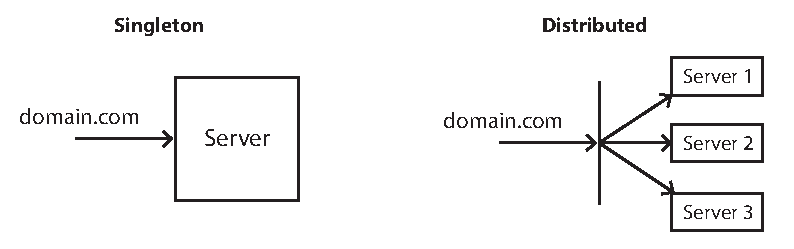
\includegraphics[width=\textwidth]{gfx/server_solutions.pdf}
    \caption{Illustration of a singleton and distributed server solution.}
    \label{fig:server_solutions}
\end{figure}

Distributed server solutions contain several servers possibly on several locations, meaning that DoS will be harder to perform, since there is no single point of failure.
However, this solution cannot ensure consistency and adds complexity.
The two solutions are graphically displayed in Figure~\ref{fig:server_solutions}.
A singleton solution has been chosen due to; consistency and simplicity.
This singleton solution will be denoted as Master or \deno{M}.

The application is required to handle communication with drones, as defined by \at{1} in Figure~\ref{tab:acceptance_tests1}.
In case of the communication being disabled, this might end up with a drone crash.
The technical limitations of antennas for digital wireless communication, sets a constraint for the availability of drones.
Assuming there exists no antenna to cover the physical area of our problem domain, it is necessary to have a distributed antenna setup in order to cover the whole physical area of the problem domain.
This leads to the structure shown in Figure~\ref{fig:antenna_structure}.

\begin{figure}[htb]
    \centering
    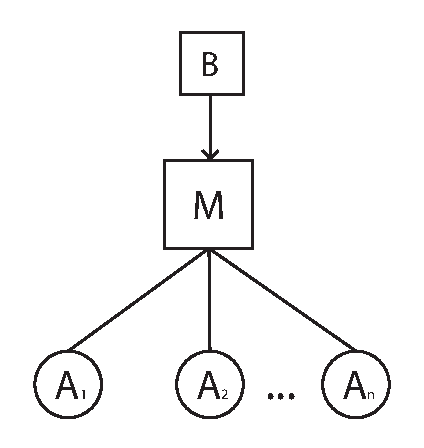
\includegraphics[width=0.5\textwidth]{gfx/antenna_structure.pdf}
    \caption{Antenna structure.}
    \label{fig:antenna_structure}
\end{figure}

If all \deno{B}'s communication with the drones goes through \deno{M}, this would create a single point of failure.
This means that, if \deno{M} crashes at any point, all communication with the drones will be disabled.
Providing the antennas with processing power and opportunity to communicate directly with \deno{B} would solve this issue.
If an antenna crashes only the drones connected to that antenna would be disconnected, leaving the drones connected to other antennas untouched.
This could be achieved by distributing some of the communication from \deno{M}.
This is solved by combining the antennas with distributed processing units, which will be denoted as Slaves or \deno{S}, as shown in Figure~\ref{fig:slave_structure}.

As \deno{S} has a dynamic network position relative to \deno{M}, this enforces that \deno{B} is not able to communicate directly with \deno{S} before getting network information about \deno{S} from \deno{M}. This communication is illustrated by a dashed line in Figure~\ref{fig:slave_structure}.

\begin{figure}[htb]
    \centering
    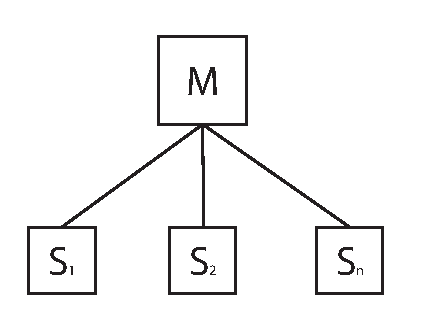
\includegraphics[width=0.5\textwidth]{gfx/slave_structure.pdf}
    \caption{Slave structure.}
    \label{fig:slave_structure}
\end{figure}

The acceptance tests, e.g. 17, 24, 25 in Figure~\ref{tab:acceptance_tests2}, enforces a constraint that requires \deno{M} to be able to store data based of the interaction of the user.
As requests can happen asynchronously, this makes it ideal to use a database denoted \deno{DB}, due to its transaction system in order to ensure no data loss.

The response output of \deno{M} needs to be dynamic based on the user, e.g. Acceptance test 2 in Figure~\ref{tab:acceptance_tests1}, which requires \deno{M} to be capable of processing data and store it in the database.
The processing unit that creates the dynamic response will be denoted \deno{W}.
The communication with the drones are handled by another processing unit, denoted \deno{D}.
If \deno{W} were to handle requests from \deno{S} and \deno{B}, this would increase the load on \deno{W}.
By creating multiple request handlers, it is possible to have a process for each. \deno{W}, \deno{DB}, and \deno{S} are processes, seen in Figure~\ref{fig:daemon_structure}, which improves resource management.
The resource management could be to constrain processing power for each process, or distribute the processes on individual machines.

\begin{figure}[htb]
    \centering
    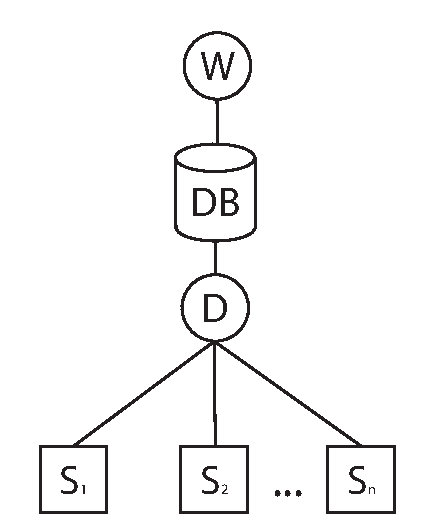
\includegraphics[width=0.5\textwidth]{gfx/daemon_structure.pdf}
    \caption{Daemon structure.}
    \label{fig:daemon_structure}
\end{figure}

% The architecture of \projectname{} differs from other web applications due to the fact that there exists two different type of servers.
% The architecture can be seen in figure~\ref{fig:system_architecture}.
% The server where the web application is running is called Master denoted M.
% For each drone in the system there is a Slave denoted S.
% On both M and S there exists daemons which is responsible for different tasks, however there is some similarity in the tasks they perform.
% These tasks can happen at anytime therefore the program needs to be running at anytime. These daemons are denoted D.
% Each user have a browser they view the application through this is denoted B.
% It is M's responsibility to communicate with every S in the system.
% S is responsible for all communication with the drone it is parred with.

% When a user wants to interact with a drone in the system a session key is needed.
% Such a session key is generated by S and then given to B through M.
% When both B and S have the same session key it is possible for them to communicate without M.
% This ensures that M does not become a bottleneck for controlling and streaming from drones and it reduces latency.
% When a new drone is added it is controlled by its S. This ensures that the system can scaled out and not have to scale up.
% Scale out means using more than one server where scale up means adding more processors, ram etc. to the server so it can handle more by itself.
% M does not handle commands and streaming, and every drone in the system have their own S.
% This makes the application architecture scalable because it removes bottlenecks from both M and S's.

% \begin{figure}[htb]
%     \centering
%     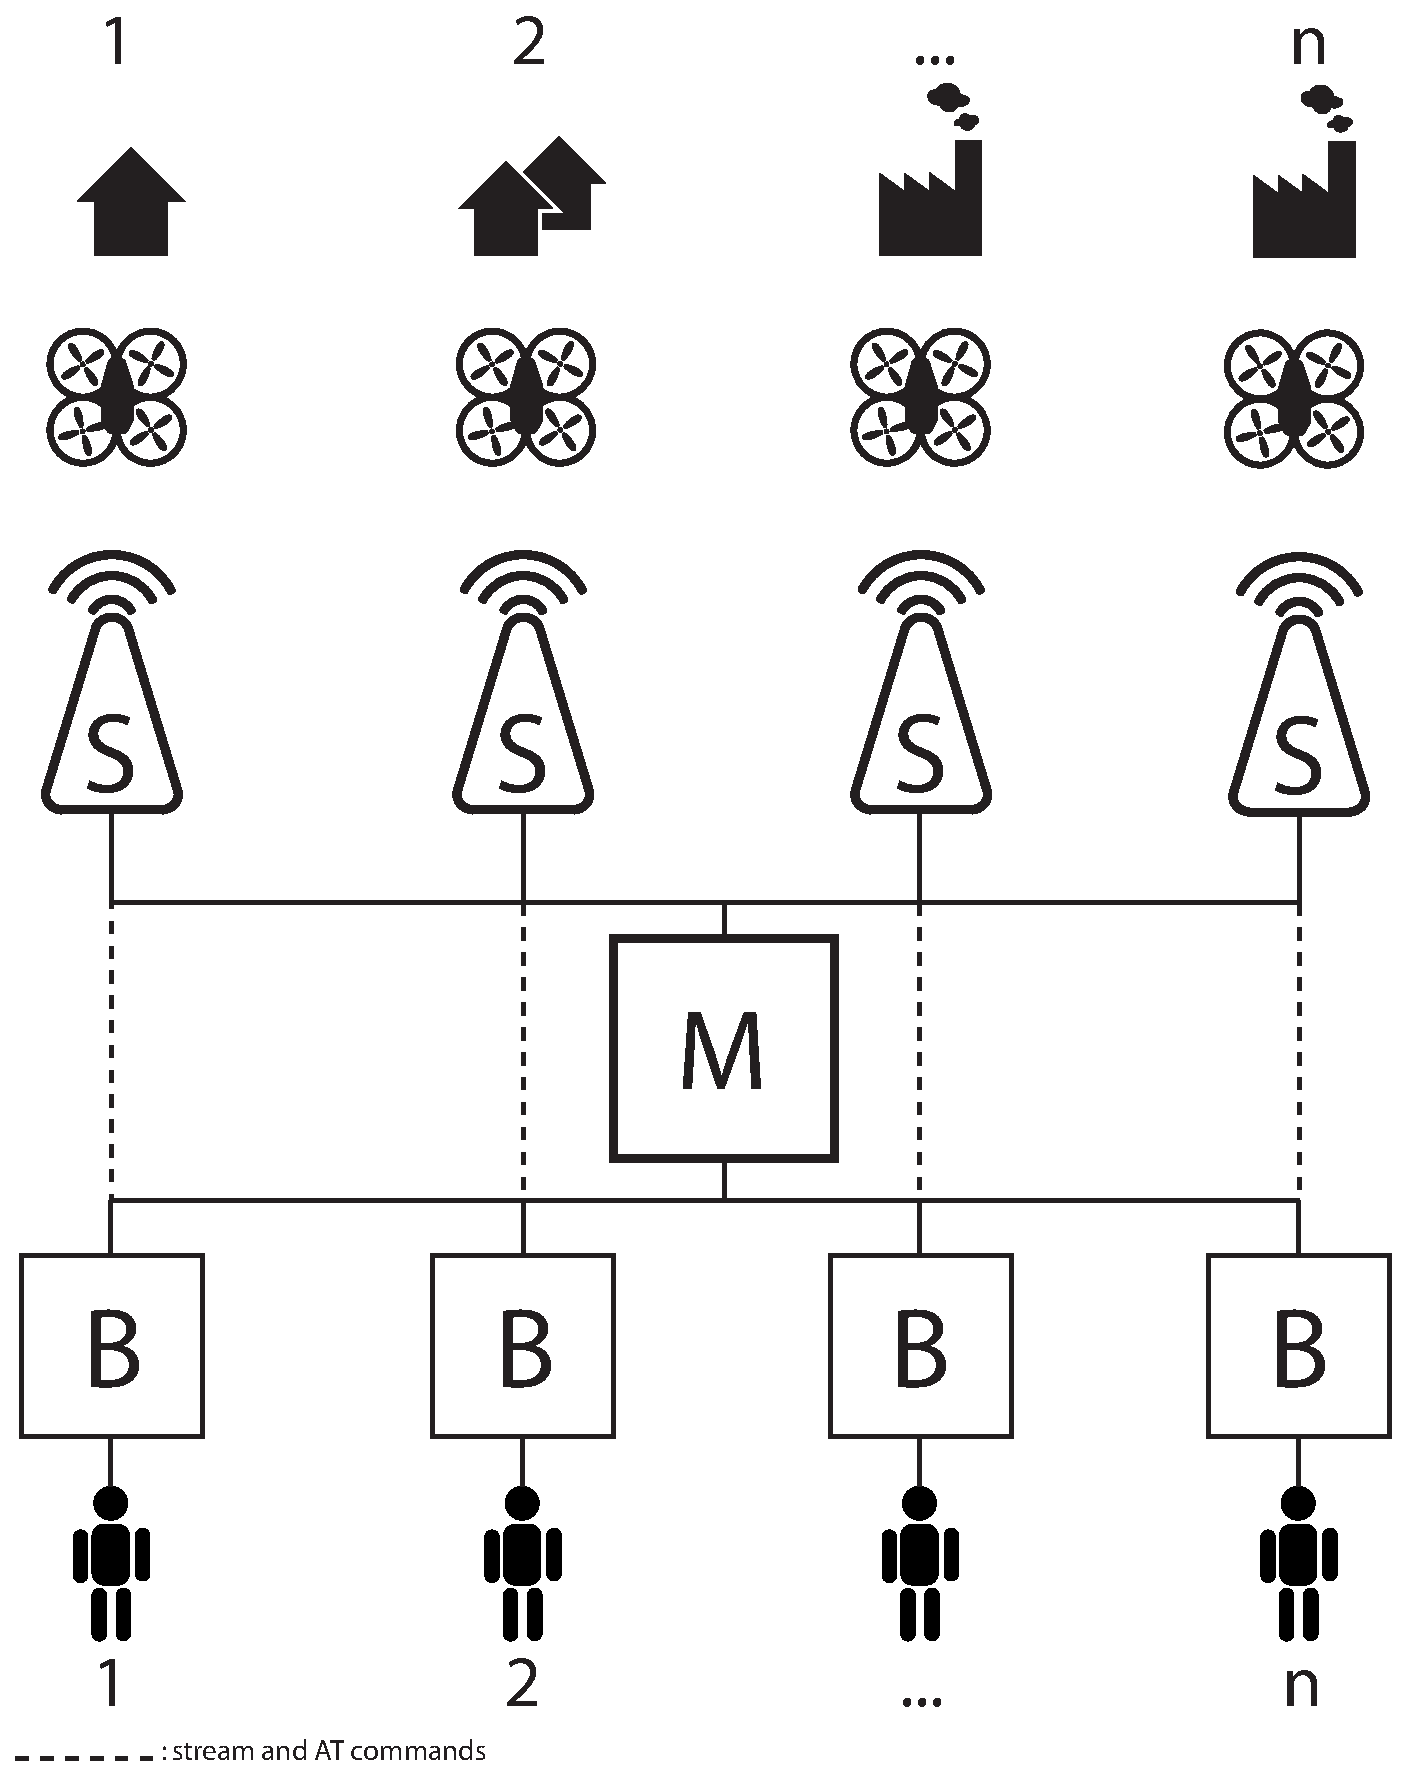
\includegraphics[width=\textwidth]{gfx/system_architecture.pdf}
%     \caption{System architecture of \projectname{}}
%     \label{fig:system_architecture}
% \end{figure}

% The system only uses one M. This can also be seen the bottleneck of the system.
% If M crashes all S's and B's will have to wait for M to come back up.
% One alternative could be running with more M's and in that way scale out.

% There is always one S for each drone connected to the system.
% In this way the system is scaled out.
% This ensures that any S is not likely to become a bottleneck.
% This was done because the drone uses wireless network which is short ranged and the drone is the host which means that the server needs one wireless connection for each drone it have to transmit to.
% One alternative could be only running with one S at each company and just scale it up.
% The problem with this is the server will need a wireless connection for each drone it have to control and it have to be in range.

% Daemon is a background process on a Linux system.
% Daemons are used when it is needed that a process is running at all times.
% In \projectname{} there are both the session key system which both resides on M and S and a policy file system for Adobe Flash on S.
% Both of these processes needs to be running at all times for the user to interact with the drone on S.
\section{Functionality distribution}\label{sec:functionality_distrubution}
% Hvilke funktionaliteter skal dækkes?
% Hvilke instancer dækker hvad?
% Hvorfor gør de det?

The functionality of the system can be derived from the acceptance tests.
This section will cover what instances are responsible for each functionality.

The need for storing data is derived from \at{1}, as previously described this is handled by the database \deno{DB}, which is a part of \deno{M}.
\at{2} sets the need for a dynamic response to \deno{B}, which requires processing of the stored data.
This processing is handled by Web or \deno{W} as the structure contains a singleton server solution.

Knowing that \deno{S} has a dynamic location relative to \deno{M}, this requires \deno{S} to send a signal to the daemon or \deno{D} in order for \deno{M} to get the location of \deno{S} on the network.
\deno{D} is then responsible for being able to receive incoming signals from \deno{S}.

Displaying video is required of \deno{B} by \at{3}.
The video displayed by \deno{B} is a stream, which requires that \deno{S} sends out a video stream.
In order to control a drone, commands have to be provided to the drone, as required by \at{3}.
\deno{S} is responsible for being able to receive commands and have the drone execute the given command.
\at{29} enforces security of the command handler.
\deno{S} is the only instance with a direct link to the drone, this makes \deno{S} responsible for the command handler's security.

% While Section~\ref{sec:application_structure} covered the overall structure of this application, this section will cover how the functionality is divided between the Master and the Slaves in the system. \\

% The Master is the users only way into the system.
% This access will always be via the users local web browser, where he sees the web system for \projectname{}.
% This web system and the database containing all informations about the system, drones, users etc. will be located on the Master.
% The Master is responsible for providing these services and coordinating the communication between the users and drones via the Slaves. \\

% A Slave is needed for every drone in the field, as the drones are not capable of long-distance communication.
% Therefore, in order to communicate with any drone, the communication must be channeled through its assigned Slave.
% This Slave is responsible for keeping contact with the drone and communicate directly with it via its API's.



\section{Communication network}\label{sec:communication_network}

Having functionality distributed across several instances sets the need for communication between the instances.
Based on Figure~\ref{fig:slave_structure}, which displays the dependency between \deno{B}, \deno{M}, and \deno{S} this leads to the diagram shown in Figure~\ref{fig:dataflow_diagrem}. \\


\begin{figure}[!h]
    \centering 
    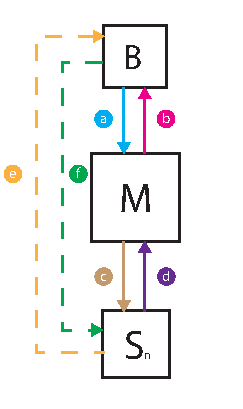
\includegraphics[width=0.5\textwidth]{gfx/dataflow_diagram.pdf}
    \caption{Dataflow diagram of \projectname{}}
    \label{fig:dataflow_diagrem}
\end{figure}


The arrows represent a connection, each connection represent dataflow in the direction of the arrow.
The type of data flowing in each connection and the reasons behind will be covered as each connection is discussed below. \\

Connection \deno{a} covers requests made by \deno{B}, which covers HTTP requests, which is a limit of web solutions that they must use the HTTP protocol.
HTTP requests enable the user to view the web application through his browser, and to send information.
In order to fulfill the request created by \deno{a}, a response is needed which the connection \deno{b} handles.
This connection covers the flow of the dynamic content created by \deno{M}, and static content such as: images, stylesheets, and multimedia objects.
Connection \deno{b} sends both the static and dynamic content back to \deno{B} to be displayed for the user. \\

The connection \deno{d} handles the signal described in Section~\ref{sec:functionality_distribution}.
This signal covers the initial communication between \deno{S} and \deno{M}. \deno{M} verifies the identity of \deno{S} by \deno{S} sending its own unique identifier.
This unique identifier is a string, which consist of X characters \fixme{How many chars?}.
All unique identifiers of each \deno{S} is known to \deno{M}.
This allows \deno{M} to determine the identity of each incoming signal. When \deno{M} receives a signal, and verify the identity of \deno{S}, the source location of the signal is stored in \deno{M} making \deno{M} able to know the location of \deno{S}. \\

Since requests from \deno{B} can happen asynchronously and from dynamic locations, it can create a problem that the identity of the connection made from \deno{S} to \deno{f} is not known. 
\at{28} sets the requirement of differentiating between incoming connections to \deno{S}.
If the communication described in connection \deno{e} and connection \deno{f} were running through \deno{M}, this would be no problem as security would be handled by the already existing sessions on \deno{M}.
The connections \deno{e} and \deno{f} are required to transport a large amount of data.
This data covers a video feed of the drone's video camera and commands for the drone.
This would increase the load on \deno{M}, which is not desired as \deno{M} is assumed to have a high load already.
However, since connection \deno{e} and connection \deno{f} are not running through \deno{M}, this leaves the problem of which \deno{B}, \deno{S} should listen to. \\

The solution chosen to solve this problem is to make \deno{S} create a randomly generated key (session key), that contains 40 characters and is unique relative to \deno{S} stored on \deno{S} itself.
When \deno{S} receives incoming commands, \deno{S} verifies whether or not the key received along with the command is equal to the one locally stored on \deno{S}.
If this is the case, \deno{S} classifies the received command as valid and performs the action.
The session key is delivered to \deno{B} from \deno{M}, as \deno{M} is able to verify the identity of \deno{B} through the session. \\

The connection \deno{c} covers requesting a session key by \deno{M}.
As \deno{M} has a static location, \deno{S} is able to verify the identity of \deno{M} based on its location.
Connection \deno{d} covers the response of the request received in \deno{c}, and \deno{M} is able to verify the identity of \deno{S} based on its location. \\

\begin{figure}[!h]
    \centering 
    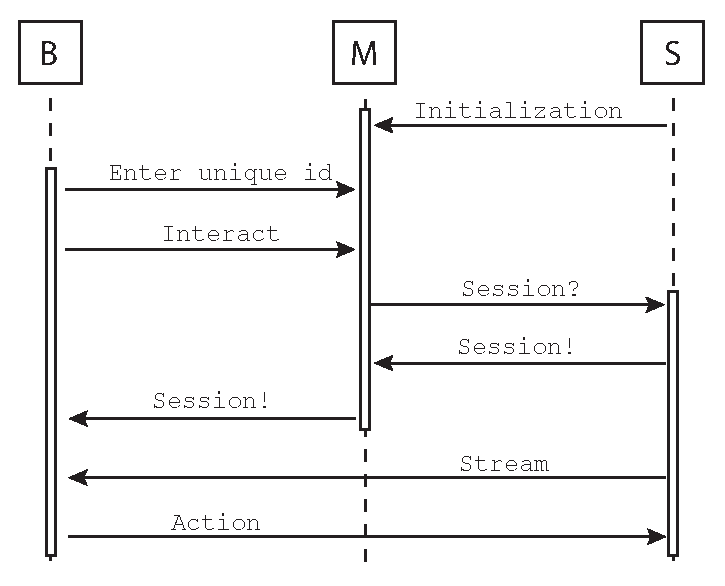
\includegraphics[width=\textwidth]{gfx/sequence_diagram.pdf}
    \caption{Sequence diagram of the communication network between \deno{B}, \deno{M}, and \deno{S}}
    \label{fig:sequence_diagram}
\end{figure}
\fxfatal{Check UML notation.}


The functionalities of the described connections, can only happen in a sequence as illustrated in Figure~\ref{fig:sequence_diagram}.
Each message in the sequence diagram can be done multiple times, however above messages are enforced to be performed atleast once in order for the given message to be performed. \\


% The communication network is crucial for \projectname{} to work.
% When designing a scalable communication network it is important to choose the right structure.
% There are different ways when designing such a network but identical for them all is that they need to support the structure of \deno{M}, \deno{S} and \deno{B} described in section~\ref{sec:application_structure}.

% One solution is to make a structure where \deno{M}, \deno{S} and \deno{B} talk to each other with a level of security. 
% The security aspect would be implemented with a form of session key. 
% This key would be used to determine if a session between a \deno{B} and a \deno{S} is valid.
% Another solution is to provide no security aspect and let it be up to the users and / or company to keep drones safe from intruders.
% This would lessen the communication between \deno{B}, \deno{M} and \deno{S}.  
% It would also decrease the load on \deno{M} and \deno{S}'s database. 
% On the down side the system could be considered not safe because it would be possible to tamper with the drones.
% As this is a system where it is important that the integrity is high, evidence is not tampered with, and where the outcome of an unauthorized user controller a drone could be devastating, it is important to deliver some form of security.



% This lead to a solution where sessions is designed to keep the integrity and secure evidence as seen in figure~\ref{fig:sequence_diagram}. 
% As seen in the figure there is designed a level of security because of the sessions.
% It is not possible for a \deno{B} to interact with a drone without having a session with a drones \deno{S}.

% When a drone is purchased a \deno{S} is setup at the location where the drone is going to operate.
% The \deno{S} sends an initializing message to \deno{M}, informing \deno{M} that a new drone has entered the system.
% \deno{M} adds the drone with the IP and location of the \deno{S}, along with the drone's unique identifier.
% If \deno{M} receives an initializing message from a \deno{S} with a drone identifier that is already in the system, it will destroy any session that correlates with that drone.
% The sessions is destroyed because if one or more sessions are granted and \deno{S} sends its initializing message it is safe to assume that \deno{S} either disconnected or crashed and all sessions keys are invalid.
% Furthermore if the IP of \deno{S} differs from the IP \deno{M} holds in its database it will be updated.

% If a user tries to interact with a drone the system behaves differently.
% A session key will be made on a \deno{S}, this key will be send to \deno{M} and giving to \deno{B}. If this session key is valid it is possible for the user to communicate directly with \deno{S} without \deno{M}.

% \begin{figure}[!h]
%     \centering 
%     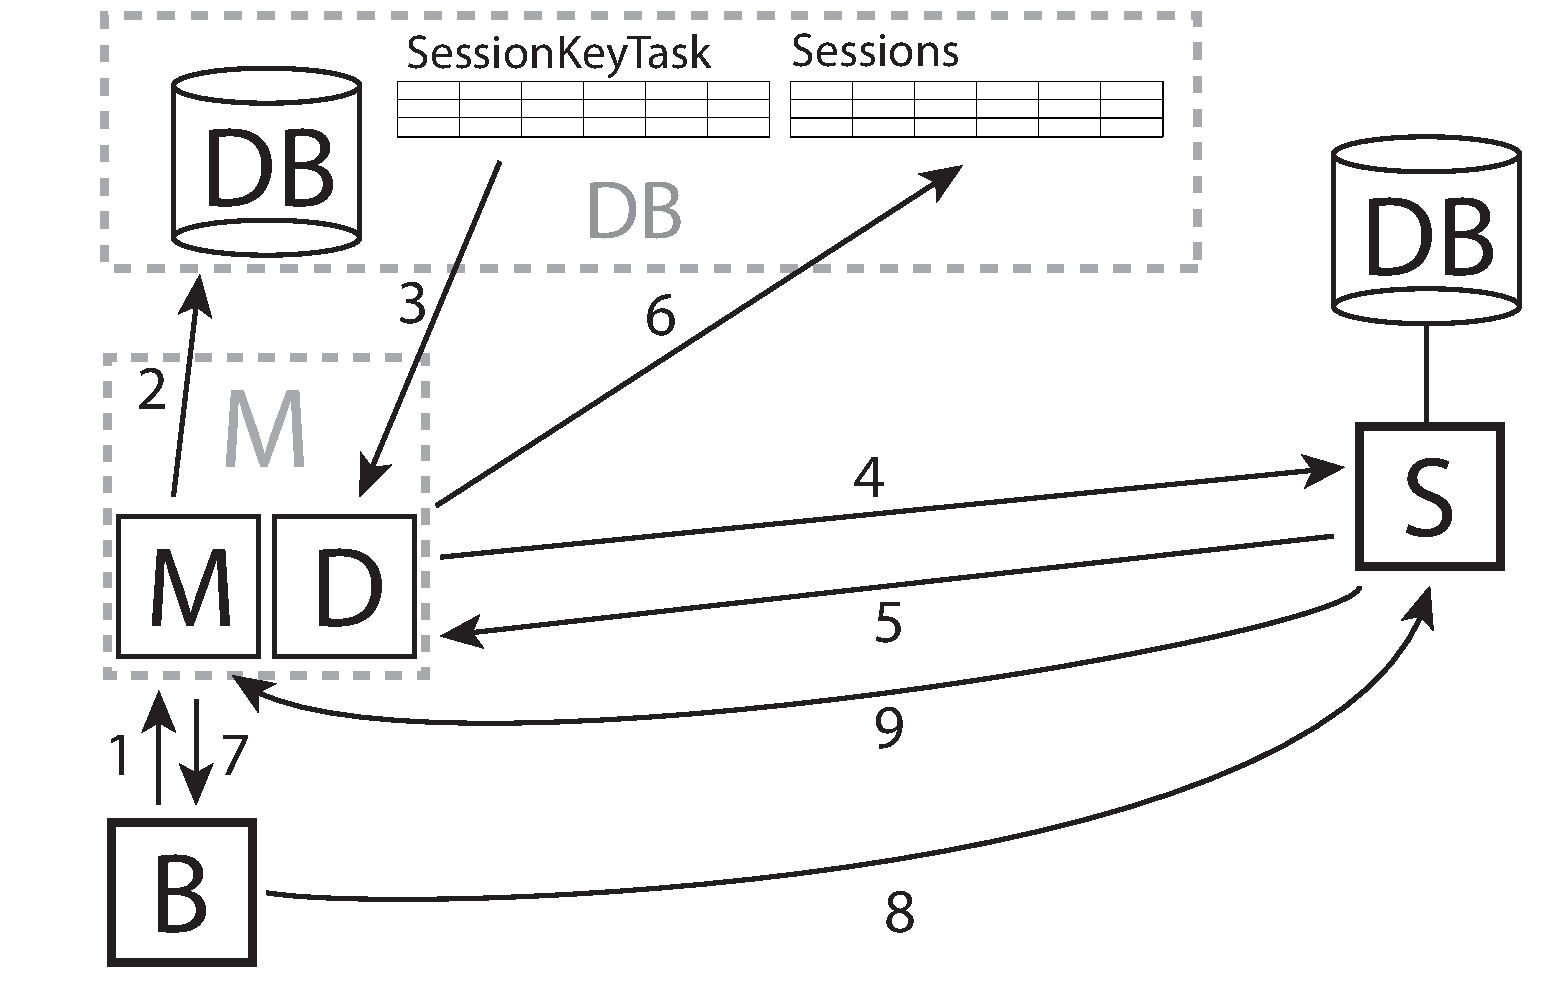
\includegraphics[width=\textwidth]{gfx/sessionkey_communication.pdf}
%     \caption{Session key communication between \deno{B}, \deno{M}, and \deno{S}}
%     \label{fig:sessionkey_communication}
% \end{figure}

% This behavior can be seen in figure~\ref{fig:sessionkey_communication}. 

% Session keys have been designed for security reasons.
% Firstly they were designed to ensure that only one user at a time can control a drone.
% Secondly it ensured that unauthorized users do not have the possibility of controlling a drone.

% \begin{enumerate}
% 	\item Request send from \deno{B} to \deno{M} about getting a session key to interact with a drone.
% 	\item \deno{M} inserts this request in its database table called SessionKeyTask.
% 	\item \deno{D} scans the database table SessionKeyTask, when it sees a new entry it select it and then deletes it from the table.
% 	\item \deno{D} requests a session key from \deno{S} parred with the drone the user wants to interact with.
% 	\item \deno{S} makes a random generated string with uppercase, lowercase letters and number. This string is used as the session key. \deno{S} updates its database with this session key and then sends it back to \deno{D} on \deno{M}.
% 	\item \deno{D} inserts the newly received session key into the session table of \deno{M}.
% 	\item \deno{M} then contacts \deno{B} with the session key.
% 	\item \deno{B} uses this session key to access \deno{S} and through it interact with the drone.
% 	\item A Timeout happens if \deno{B} and \deno{S} does not communicate for 10 seconds.
% \end{enumerate}

% Communication between the servers in the system is crucial. 
% Therefore it is important design a method or a set of methods handling the communication between them. 
% One method could be to make a service which handles all these requests on each server.
% The problem however is that using a single service might create a bottleneck.
% An alternative solution is to make a service for each communication level.
% One service that handles sessions, a service that handles control commands, and a service that handles initial messages from \deno{S} see section~\ref{sec:application_structure}.\fxfatal{Den her paragraf er uspecifik}

% This lead to a solution where the different actors in the system delivered and / or depended on services.

% The interface of the communication network can be seen in figure~\ref{fig:communication_network}.

% The communication network of \projectname{} uses four different ports for providing its services:

% \begin{itemize}
% 	\item Port A - service port for sending and receiving drone control commands.
% 	\item Port B - service port for receiving and sending initial messages.
% 	\item Port C - service port for sending and receiving session information including session keys.
% 	\item Port Web - service port for sending and receiving web specific information.
% \end{itemize}

% \begin{figure}[!h]
%     \centering 
%     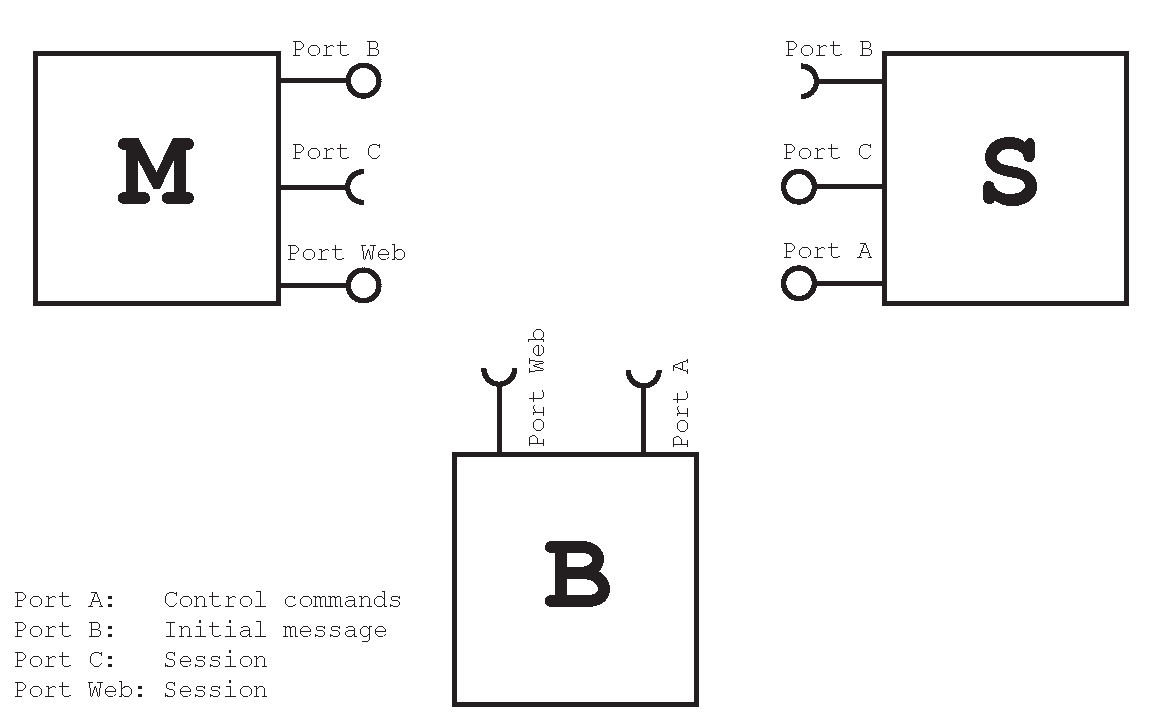
\includegraphics[width=\textwidth]{gfx/communication_network.pdf}
%     \caption{Communication network between \deno{B}, \deno{M}, and \deno{S}}
%     \label{fig:communication_network}
% \end{figure}

% When designing a communication network it is also important to select the right technique for exchanging data between services.
% One of the more widely used techniques are Extensible Markup Language.
% Extensible Markup Language, or XML for short, is a markup language designed to easily mark up data.
% The markup that XML provides makes it possible to easily send and receive data.
% The Extensible in XML makes it possible to extent what data types XML can handle through the XML schema. \citep{simonstl}
% This gives XML a drawback because XML is designed to be extensible it also carries a lot of overhead when used to mark up data.

% \projectname{} needs to be scalable therefore it is important to use as little overhead when sending structured information.
% Otherwise there is a chance that this overhead creates a bottleneck within the network.

% JSON, or JavaScript Object Notation, is design for data interchange and to be human-readable.
% It have a simpler syntax than XML and is not build to be extensible, it is not even a markup language. 
% It is a structured way of exchanging data between sources. 
% This results in less overhead i.e. it costs less data for each piece of information. 
% JSON is also data orientated which makes it easier to map a JSON object directly to a object orientated structure.
% Douglas Crockford call JSON ``The Fat-Free Alternative to XML'' \citep{JSON}.

% Therefore JSON is the perfect format for data interchange between the different services in \projectname{}. There are lesser costs associated with JSON than XML and it is easier to map them into a object orientated language.
\section{Object Model}
\label{section:uml_notation}
\label{subsec:objects}

This section will cover the design choices behind the application's object model, derived from the use cases in Section~\ref{sec:use_cases}.
The UML object model diagram can be seen in Figure~\ref{fig:UML_class_diagram}, and is guided by the UML standard guide written in cooperation by several different software companies~\citep{UML_notation}.\\

The UML attribute notation in this report is:
\begin{itemize}
    \item PK attribute - means that the attribute is a primary key.
    \item FK attribute - means that the attribute is a foreign key.
    \item attribute : type - all attributes will have a type e.g. \verb+id : int+.
\end{itemize}

The system will contain the following objects: \deno{Affiliate Privilege}, \deno{Company}, \deno{Drone}, \deno{Privilege}, \deno{Role}, \deno{Session}, and \deno{User}.
The model of the objects and their relationships can be seen in Figure~\ref{fig:UML_class_diagram}.
Each object covered is represented in the object model diagram with its name in lowercase and pluralized, e.g. \deno{User} object $\rightarrow$ \deno{users}.
If an object's name consists of several words the spaces will be replaced by underscores, e.g. Session Key Task becomes session\_key\_tasks.
The relationships between objects can either be implicit with a line directly from one object to another, or explicit with a simple or rich relationship model between the two objects.
Simple relationship models are models without a PK.
They are represented in the model diagram with both objects in lowercase and pluralized, e.g. roles\_users.
Rich relationship models have a PK.
This kind of relationship model does not have a predetermined naming convention, therefore it can be anything as long as it does not collide with the other model names, e.g. user\_privileges.\\

\begin{figure}[htb]
    \centering
    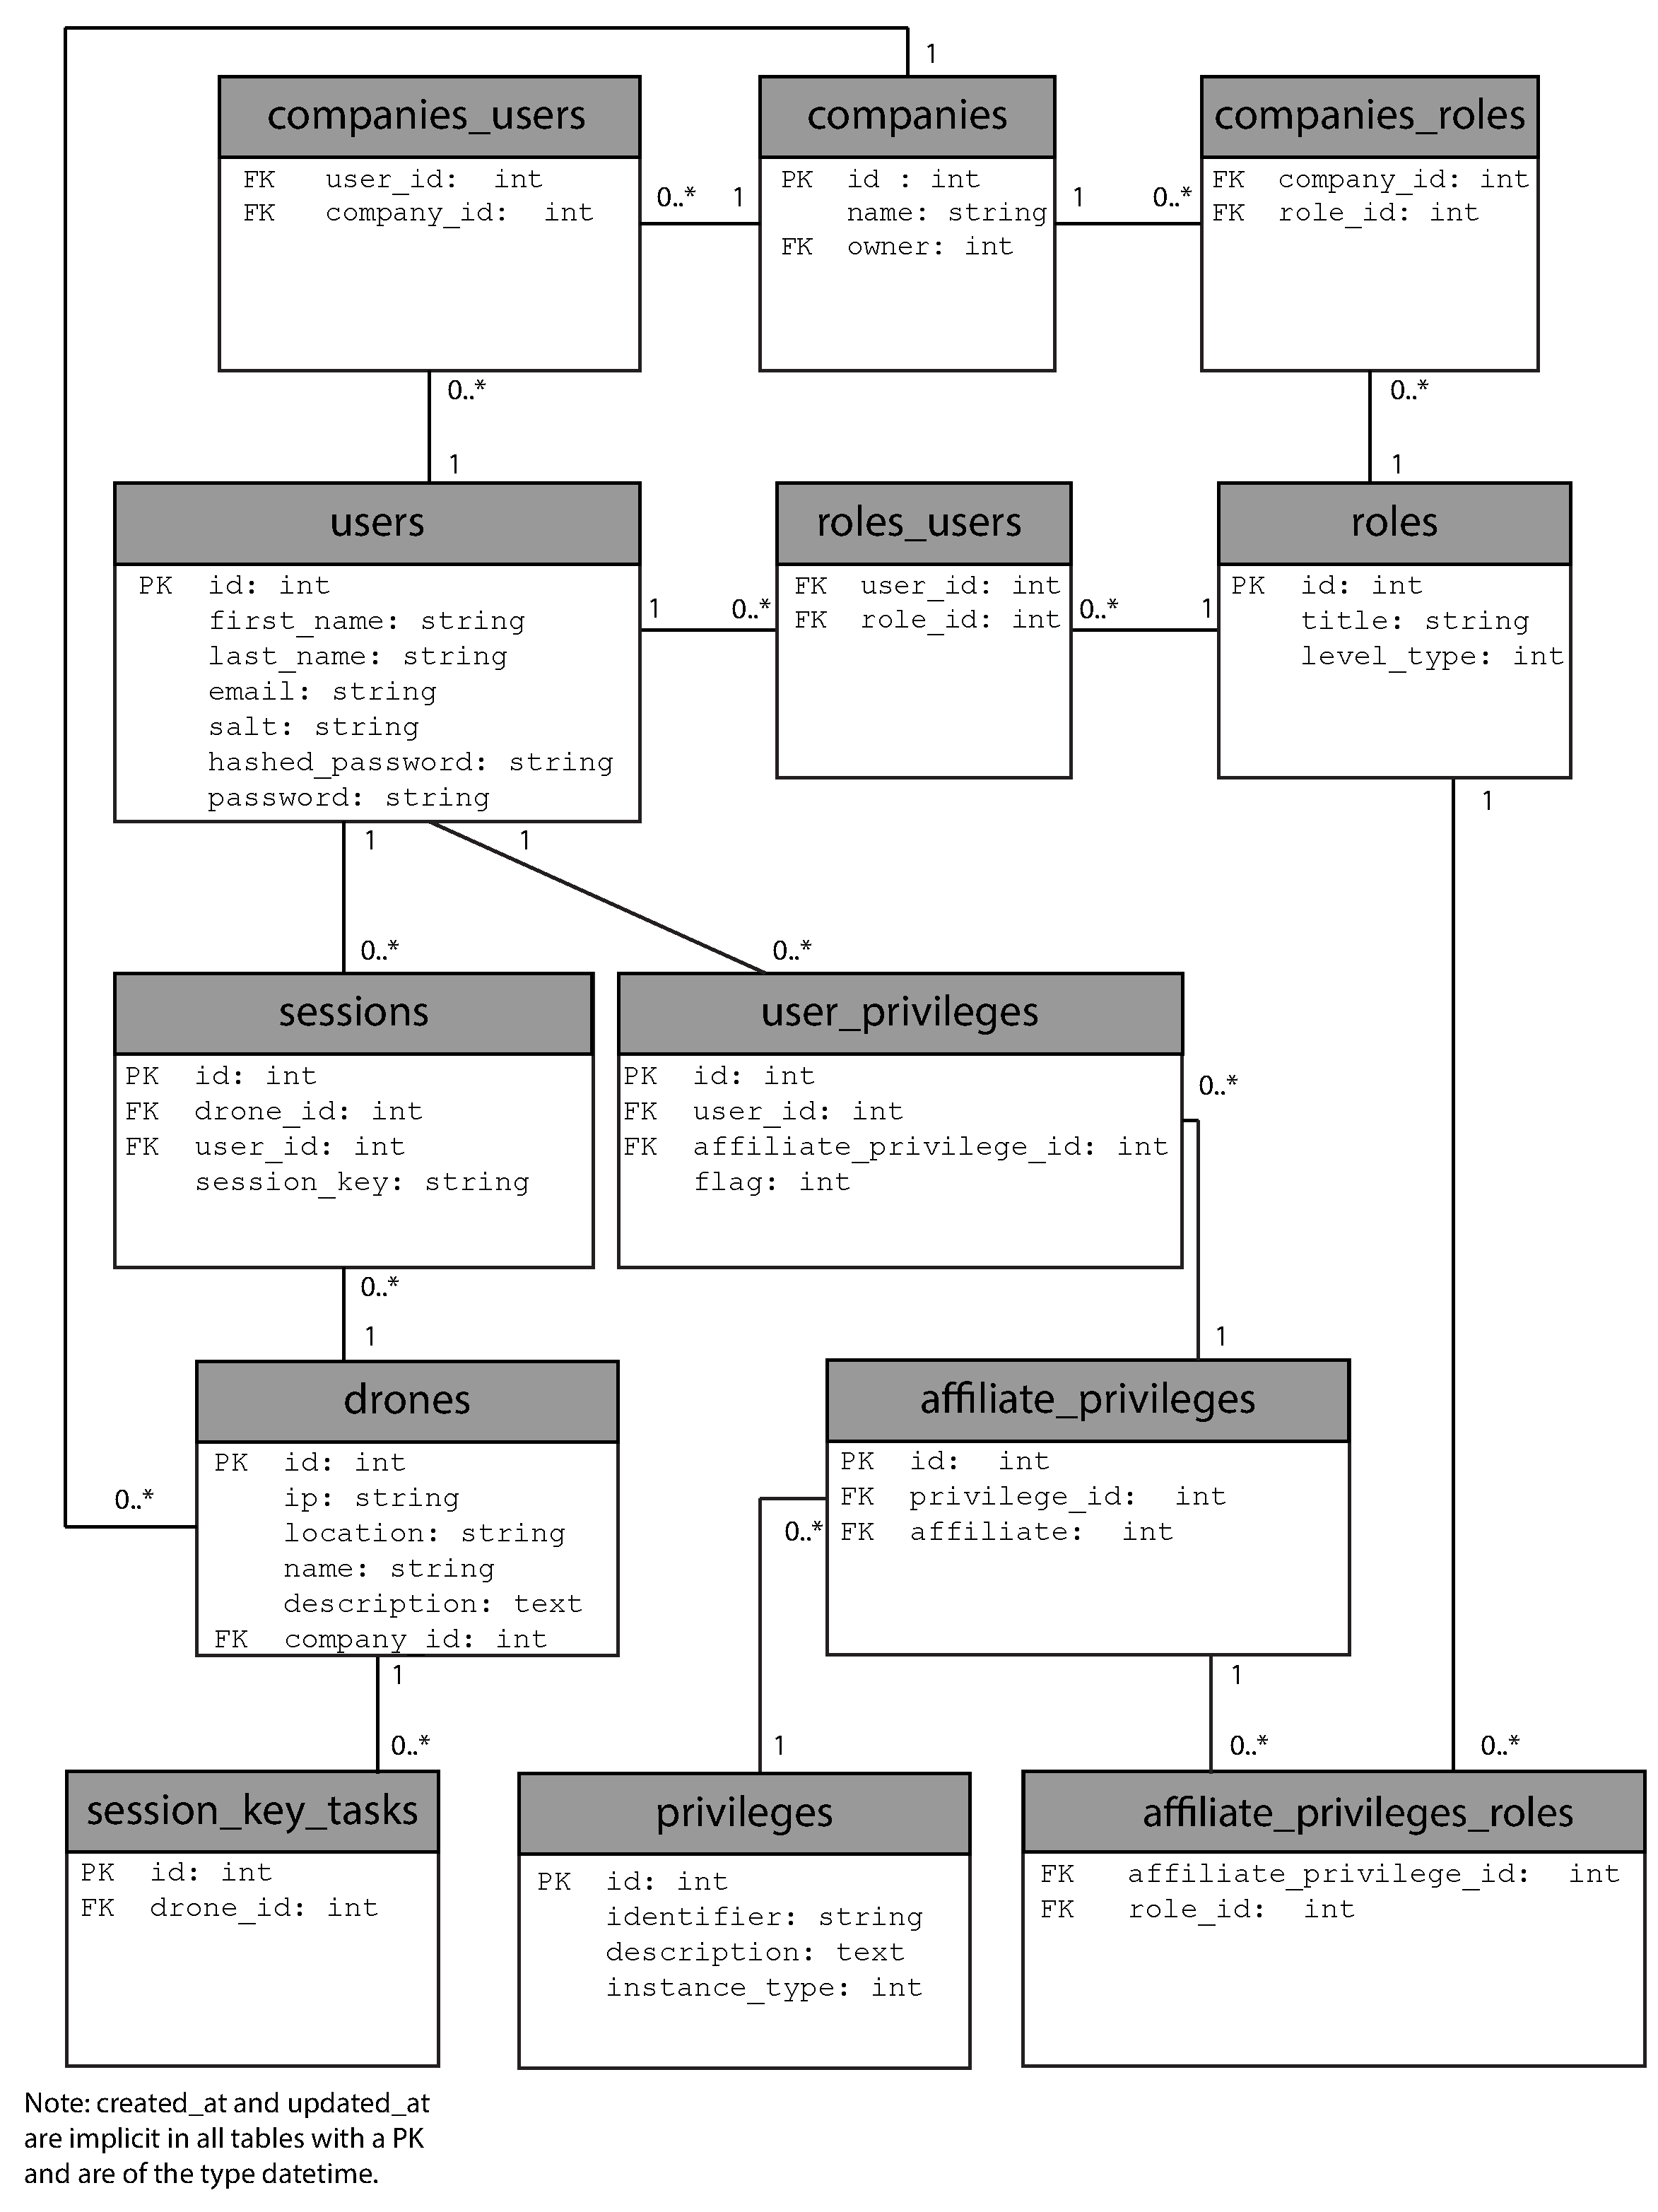
\includegraphics[width=0.95\textwidth]{gfx/UML_model.pdf}
    \caption{UML Class Diagram of \projectname{}}
    \label{fig:UML_class_diagram}
\end{figure}


\subsection{Objects}\fixme{Skal denne overskrift være der? Det burde ikke være nødvendigt at have den, men så skal teksten ændres lidt.}
Access to and actions of the system is restricted.
This restriction is based on the identity of user in the system.
An instance of the \deno{User} object represents a user to the system.
The \deno{User} object has the attributes \verb+email+ and \verb+password+, as seen in Figure~\ref{tab:user_object} in Appendix~\ref{app:objects}, these combined form the login credentials needed for a user to authenticate his identity towards the system. \\

The \verb+email+ is publicly available, which leaves the \verb+password+ to be protected in order for user to protect his identity in the system.
The \verb+password+ entered by the user is concatenated with a \verb+salt+ and hashed through a SHA-1 hashing algorithm to be stored in \verb+hashed_password+.
The hashing algorithm provides a way for storing the password without having its exact value, as this could leave to a security flaw.
Having access to passwords of users directly, e.g. through a hacker attack, would allow the hacker to login into the users account, which is unintended for the system.
When a salt is concatenated before hashing it makes it harder for the hacker to gain the original passwords, e.g. through a rainbow table~\cite{something}. \\

Having a distributed setup with multiple \deno{S}, each representing a \deno{Drone} object, means that the network locations of these need to be known in order to communicate.
The network location is stored in the \verb+ip+ field of the \deno{Drone} object, as shown in Figure~\ref{tab:drone_object} of Appendix~\ref{app:objects}.
The physical drone have a unique identifier known as \verb+name+, which makes the user able to identify a given drone. \\

The users of the system will be part of different companies, therefore there is a need for grouping users by a company.
The \deno{Company} object have an \verb+owner+, which is a reference to a \deno{User} object.
This is required for the system to know which user have access to all \deno{Affiliate Privilege} objects of the company. \\

An \deno{Affiliate Privilege} object references a \deno{Privilege}, and only when combined they form a unique key.
This key unlocks a certain functionality, meaning that if the user does not have a relation to the \deno{Affiliate Privilege} object, which represents the key, then the user is not able to unlock that functionality.
\deno{Role} objects give the possibility of grouping \deno{Privilege} objects together.
Each \deno{Company} have a related role which contains all privileges, of which the company have full control.
Full control gives the right for passing on a privilege, or disabling if the privilege is already granted.
\deno{Affiliate Privilege} objects have a field \verb+affiliate+ that links the privilege to an object of the type declared by the referenced \deno{Privilege} object's \verb+instance_type+ field. \\

The \deno{Session} object represents an active pilot connection between a user and a drone.
The \verb+session_key+ field provides a key that needs to be sent along with the commands.
The \deno{Session Key Task} object is an object used for \deno{D} and \deno{M} to communicate through \deno{DB}, as shown in Figure~\ref{fig:daemon_structure} in Section~\ref{sec:application_structure}. \\

In Section~\ref{sec:privileges} solutions for handling privileges were discussed.
From this discussion it was decided to model a system capable of handling all proposed solutions to fit scenarios of the users.
The \deno{User Privileges} relationship allows for connecting individual {Privilege} objects to a \deno{User} object.
This is could be either granting or revoking, i.e. exceptions, the privilege.
The \verb+flag+ field represents a value of either 1 or -1; 1 is regarded as granted, and -1 is regarded as revoked.


% \subsection{Relationships}
% The system is designed with flexibility and scalability in mind, and the structure of Roles and Privileges are what provides those features.
% As described before there are two ways that a User can be granted a specific Privilege.
% These are by 1) getting the Privilege granted directly via the \verb+User_Privileges+ table or 2) by being a member of a Role that via the \verb+Privileges_Roles+ table that has one or more Privileges granted.
% These will be explained in details in the following subsections.


% % Users and Privileges %
% An administrator can grant a specific Privilege directly to a user via the \verb+User_Privileges+ table.
% This Privilege is then affiliated with an object -- usually a Drone.
% The Privilege could also be a system functionality, however, as described in Section~\ref{sec:privileges}. \\

% This relationship is also used for exceptions.
% In an example where five Users: U1, U2, U3, U4 and U5 are a member of a Role: R1, we may have a situation where U2 is not suppose to have access to a given Privilege P1 in R1.
% Then a User-specific Privilege is granted to U2 on P1, but with the ``exception''-flag marked.
% This is equal to blacklisting U2 from using Privilege P1, providing the system with a lot of flexibility, as even though a group of Users are granted a number of Privileges via a role, User-specific exceptions can be added to this setting. \\


% % Roles and Privileges %
% As mentioned before -- the reason that Roles can be used to assign Privileges to a User, is to make both the administration and data structure of Users and Privileges as simple and efficient as possible.
% By allowing exceptions, full flexibility is still possible. \\

% This is how the relationship between Roles and Privileges works: \\

% An administrator creates a Role.
% Lets call this Role ``Control Drone \#4''.
% A number of Privileges are assigned to this Role.
% It could be the following:

% \begin{itemize}
%     \item Watch the video feed from a specific drone
%     \item Control the movement of a specific drone
% \end{itemize}

% Those Privileges are then linked to this Role and to the Drone this concerns. \\

% Roles can be assigned with affiliation to both Users and Companies.
% Say a user \verb+U1+ needs access to Drone \#4.
% User U1 then needs to either have the Privileges directly granted or be a member of the role ``Control Drone \#4''.


% % Privileges and granting of Privileges %
% Since it is possible to grant Privileges both directly to a User and via a Role, the same Privilege can be used in more than one context.
% Therefore the \verb+Affiliation_Privileges+ table exists.
% This table links the granting of a Privilege with the actual Privilege and defines on which Object the Privilege applies.
% The reason for having this table and not just link the two granting-tables \verb+User_Privileges+ and \verb+Privileges_Roles+ directly to the \verb+Privileges+ table, is that we try to avoid redundant data by having the data in the \verb+Privileges+ and \verb+Affiliation_Privileges+ table make up one instance of a privilege together.
% This is then granted to a User or a Role, who can then use the Privilege. \\

% The system is designed so that any User can grant a Privilege he already has already been granted to another User if he is permitted to.
% This is controlled via a ``re-grantable'' flag which is set in either the \verb+User_Privileges+ table or the \verb+Privileges_Roles+ table.
% By marking this flag as ``true'', the User or Users that via a Role is granted the Privilege in question, can via an interface in the system re-grant the Privilege to other Users in the same Company.


% %Note: Alle brugere kan videregrante et privilege hvis de har tilladelse til det. Det er et flag som sætes i user_privileges og privileges_roles, som tillader alle der har dette privilegie til at videregrante det. Husk at beskrive hvordan et privilege og et affiliation privilege til sammen giver et grant-able privilegie


% % Privileges and Drones %
% With \projectname{} in its current form, most Privileges that are granted will have an connected with a Drone.
% Privileges and its a affiliations are linked in the \verb+Affiliation_Privileges+ table.
% This is also where Drones are linked to any granted privilege. \\

% As described earlier, Drones are the current object-type implemented in the system.
% However, the structure and model of the system allows for later expansion, connection new objects such as stationary cameras or any other type of object to the system.
% The \verb+Affiliation_Privileges+ has a third field named \verb+object_id+.
% This field links the Privilege, the granting of it and the Object that this granting is valid for. \\

% An example could be linking Privilege P1, User U1 and Drone D1.
% Say P1 is the privilege for watching the video feed of a drone.
% Then the user U1 will have access to watch the video feed of Drone D1.


% % Drones and Companies %
% The \verb+Company_drones+ table defines a relationship between a Drone and a Company.

% The administrator of each Company defines the Roles in that Company.
% In doing so, he defines which Privileges that are granted in every Role.
% These Privileges are linked to a (Drone)-object.
% The system must make sure that any Company administrator cannot link a Privilege with a Object that is not within his control. \\

% This relationship defines which Drones are available to each Company.
% When a Company administrator adds new Roles (and hence Privileges), he is only able to associate it with Drones that are connected to the Company in question.

% **************************************************************************************************************
% A Classic Thesis Style
% An Homage to The Elements of Typographic Style
%
% Copyright (C) 2012 Andr\'e Miede http://www.miede.de
%
% If you like the style then I would appreciate a postcard. My address
% can be found in the file ClassicThesis.pdf. A collection of the
% postcards I received so far is available online at
% http://postcards.miede.de
%
% License:
% This program is free software; you can redistribute it and/or modify
% it under the terms of the GNU General Public License as published by
% the Free Software Foundation; either version 2 of the License, or
% (at your option) any later version.
%
% This program is distributed in the hope that it will be useful,
% but WITHOUT ANY WARRANTY; without even the implied warranty of
% MERCHANTABILITY or FITNESS FOR A PARTICULAR PURPOSE.  See the
% GNU General Public License for more details.
%
% You should have received a copy of the GNU General Public License
% along with this program; see the file COPYING.  If not, write to
% the Free Software Foundation, Inc., 59 Temple Place - Suite 330,
% Boston, MA 02111-1307, USA.
%
% **************************************************************************************************************
% Note:
%    * You must not use "u etc. in strings/commands that will be spaced out (use \"u or real umlauts instead)
%    * New enumeration (small caps): \begin{aenumerate} \end{aenumerate}
%    * For margin notes: \marginpar or \graffito{}
%    * Do not use bold fonts in this style, it is designed around them
%    * Use tables as in the examples
%    * See classicthesis-preamble.sty for useful commands
% **************************************************************************************************************
% To Do:
%		 * [high] Check this out: http://www.golatex.de/koma-script-warnung-in-verbindung-mit-listings-package-t2058.html
%    * [medium] mathbb in section-titles/chapter-titles => disappears somehow in headlines!!!
% **************************************************************************************************************
\documentclass[ twoside,openright,titlepage,numbers=noenddot,headinclude,%1headlines,% letterpaper a4paper
                footinclude=true,cleardoublepage=empty,abstractoff, % <--- obsolete, remove (todo)
                BCOR=5mm,paper=a4,fontsize=11pt,%11pt,a4paper,%
                ngerman,american,%
                ]{scrreprt}

%********************************************************************
% Note: Make all your adjustments in here
%*******************************************************
% ****************************************************************************************************
% classicthesis-config.tex
% formerly known as loadpackages.sty, classicthesis-ldpkg.sty, and classicthesis-preamble.sty
% Use it at the beginning of your ClassicThesis.tex, or as a LaTeX Preamble
% in your ClassicThesis.{tex,lyx} with \input{classicthesis-config}
% ****************************************************************************************************
% If you like the classicthesis, then I would appreciate a postcard.
% My address can be found in the file ClassicThesis.pdf. A collection
% of the postcards I received so far is available online at
% http://postcards.miede.de
% ****************************************************************************************************

% ****************************************************************************************************
% 1. Configure classicthesis for your needs here, e.g., remove "drafting" below
% in order to deactivate the time-stamp on the pages
% ****************************************************************************************************
\PassOptionsToPackage{eulerchapternumbers,listings,drafting,%
				 pdfspacing,%floatperchapter,%linedheaders,%
				 subfig,beramono,eulermath,parts}{classicthesis}
% ********************************************************************
% Available options for classicthesis.sty
% (see ClassicThesis.pdf for more information):
% drafting
% parts nochapters linedheaders
% eulerchapternumbers beramono eulermath pdfspacing minionprospacing
% tocaligned dottedtoc manychapters
% listings floatperchapter subfig
% ********************************************************************

% ********************************************************************
% Triggers for this config
% ********************************************************************
\usepackage{ifthen}
\newboolean{enable-backrefs} % enable backrefs in the bibliography
\setboolean{enable-backrefs}{false} % true false
% ****************************************************************************************************


% ****************************************************************************************************
% 2. Personal data and user ad-hoc commands
% ****************************************************************************************************
\newcommand{\myTitle}{LONE\xspace}
\newcommand{\mySubtitle}{Lone is Observation of Nondeterministic Environments\xspace}
%\newcommand{\myDegree}{Doktor-Ingenieur (Dr.-Ing.)\xspace}
\newcommand{\myName}{SW701E12\xspace}
\newcommand{\myProf}{Put name here\xspace}
\newcommand{\myOtherProf}{Put name here\xspace}
\newcommand{\mySupervisor}{Put name here\xspace}
\newcommand{\myFaculty}{Put data here\xspace}
\newcommand{\myDepartment}{Put data here\xspace}
\newcommand{\myUni}{Aalborg University\xspace}
\newcommand{\myLocation}{Aalborg\xspace}
\newcommand{\myTime}{December 2012\xspace}
\newcommand{\myVersion}{version 4.1\xspace}
\newcommand{\projectname}{<projectname>}

% ********************************************************************
% Setup, finetuning, and useful commands
% ********************************************************************
\newcounter{dummy} % necessary for correct hyperlinks (to index, bib, etc.)
\newlength{\abcd} % for ab..z string length calculation
\providecommand{\mLyX}{L\kern-.1667em\lower.25em\hbox{Y}\kern-.125emX\@}
\newcommand{\ie}{i.\,e.}
\newcommand{\Ie}{I.\,e.}
\newcommand{\eg}{e.\,g.}
\newcommand{\Eg}{E.\,g.}
% ****************************************************************************************************


% ****************************************************************************************************
% 3. Loading some handy packages
% ****************************************************************************************************
% ********************************************************************
% Packages with options that might require adjustments
% ********************************************************************
\PassOptionsToPackage{latin9}{inputenc}	% latin9 (ISO-8859-9) = latin1+"Euro sign"
 \usepackage{inputenc}

%\PassOptionsToPackage{ngerman,american}{babel}   % change this to your language(s)
% Spanish languages need extra options in order to work with this template
%\PassOptionsToPackage{spanish,es-lcroman}{babel}
 \usepackage{babel}

\PassOptionsToPackage{square,numbers}{natbib}
 \usepackage{natbib}

\PassOptionsToPackage{fleqn}{amsmath}		% math environments and more by the AMS
 \usepackage{amsmath}

% ********************************************************************
% General useful packages
% ********************************************************************
\PassOptionsToPackage{T1}{fontenc} % T2A for cyrillics
	\usepackage{fontenc}
\usepackage{textcomp} % fix warning with missing font shapes
\usepackage{scrhack} % fix warnings when using KOMA with listings package
\usepackage{xspace} % to get the spacing after macros right
\usepackage{mparhack} % get marginpar right
\usepackage{fixltx2e} % fixes some LaTeX stuff
\PassOptionsToPackage{printonlyused,smaller}{acronym}
	\usepackage{acronym} % nice macros for handling all acronyms in the thesis
%\renewcommand*{\acsfont}[1]{\textssc{#1}} % for MinionPro
\renewcommand{\bflabel}[1]{{#1}\hfill} % fix the list of acronyms
\usepackage[footnote,draft,english,silent,nomargin]{fixme}  % final instead of draft produces errors at
                                                            % compile time
                                                            
%Bjarke HS stuff
\newcommand{\todo}[1]{\fxnote{#1}}
\newcommand{\todoi}[1]{\fxfatal{#1}}
\newcommand{\todoI}[1]{\todoi{#1}}

%Rasmus stuff
\newcommand{\figref}[1]{\figurename~\ref{#1}}

% ****************************************************************************************************


% ****************************************************************************************************
% 4. Setup floats: tables, (sub)figures, and captions
% ****************************************************************************************************
\usepackage{tabularx} % better tables
	\setlength{\extrarowheight}{3pt} % increase table row height
\newcommand{\tableheadline}[1]{\multicolumn{1}{c}{\spacedlowsmallcaps{#1}}}
\newcommand{\myfloatalign}{\centering} % to be used with each float for alignment
\usepackage{caption}
\captionsetup{format=hang,font=small}
\usepackage{subfig}
% ****************************************************************************************************


% ****************************************************************************************************
% 5. Setup code listings
% ****************************************************************************************************
\usepackage{listings}
%\lstset{emph={trueIndex,root},emphstyle=\color{BlueViolet}}%\underbar} % for special keywords
\lstset{language=[LaTeX]Tex,%C++,
    keywordstyle=\color{RoyalBlue},%\bfseries,
    basicstyle=\small\ttfamily,
    %identifierstyle=\color{NavyBlue},
    commentstyle=\color{Green}\ttfamily,
    stringstyle=\rmfamily,
    numbers=none,%left,%
    numberstyle=\scriptsize,%\tiny
    stepnumber=5,
    numbersep=8pt,
    showstringspaces=false,
    breaklines=true,
    frameround=ftff,
    frame=single,
    belowcaptionskip=.75\baselineskip
    %frame=L
}
% ****************************************************************************************************


% ****************************************************************************************************
% 6. PDFLaTeX, hyperreferences and citation backreferences
% ****************************************************************************************************
% ********************************************************************
% Using PDFLaTeX
% ********************************************************************
\PassOptionsToPackage{pdftex,hyperfootnotes=false,pdfpagelabels}{hyperref}
	\usepackage{hyperref}  % backref linktocpage pagebackref
\pdfcompresslevel=9
\pdfadjustspacing=1
\PassOptionsToPackage{pdftex}{graphicx}
	\usepackage{graphicx}

% ********************************************************************
% Setup the style of the backrefs from the bibliography
% (translate the options to any language you use)
% ********************************************************************
\newcommand{\backrefnotcitedstring}{\relax}%(Not cited.)
\newcommand{\backrefcitedsinglestring}[1]{(Cited on page~#1.)}
\newcommand{\backrefcitedmultistring}[1]{(Cited on pages~#1.)}
\ifthenelse{\boolean{enable-backrefs}}%
{%
		\PassOptionsToPackage{hyperpageref}{backref}
		\usepackage{backref} % to be loaded after hyperref package
		   \renewcommand{\backreftwosep}{ and~} % separate 2 pages
		   \renewcommand{\backreflastsep}{, and~} % separate last of longer list
		   \renewcommand*{\backref}[1]{}  % disable standard
		   \renewcommand*{\backrefalt}[4]{% detailed backref
		      \ifcase #1 %
		         \backrefnotcitedstring%
		      \or%
		         \backrefcitedsinglestring{#2}%
		      \else%
		         \backrefcitedmultistring{#2}%
		      \fi}%
}{\relax}

% ********************************************************************
% Hyperreferences
% ********************************************************************
\hypersetup{%
    %draft,	% = no hyperlinking at all (useful in b/w printouts)
    colorlinks=true, linktocpage=true, pdfstartpage=3, pdfstartview=FitV,%
    % uncomment the following line if you want to have black links (e.g., for printing)
    %colorlinks=false, linktocpage=false, pdfborder={0 0 0}, pdfstartpage=3, pdfstartview=FitV,%
    breaklinks=true, pdfpagemode=UseNone, pageanchor=true, pdfpagemode=UseOutlines,%
    plainpages=false, bookmarksnumbered, bookmarksopen=true, bookmarksopenlevel=1,%
    hypertexnames=true, pdfhighlight=/O,%nesting=true,%frenchlinks,%
    urlcolor=webbrown, linkcolor=RoyalBlue, citecolor=webgreen, %pagecolor=RoyalBlue,%
    %urlcolor=Black, linkcolor=Black, citecolor=Black, %pagecolor=Black,%
    pdftitle={\myTitle},%
    pdfauthor={\textcopyright\ \myName, \myUni, \myFaculty},%
    pdfsubject={},%
    pdfkeywords={},%
    pdfcreator={pdfLaTeX},%
    pdfproducer={LaTeX with hyperref and classicthesis}%
}

% ********************************************************************
% Setup autoreferences
% ********************************************************************
% There are some issues regarding autorefnames
% http://www.ureader.de/msg/136221647.aspx
% http://www.tex.ac.uk/cgi-bin/texfaq2html?label=latexwords
% you have to redefine the makros for the
% language you use, e.g., american, ngerman
% (as chosen when loading babel/AtBeginDocument)
% ********************************************************************
\makeatletter
\@ifpackageloaded{babel}%
    {%
       \addto\extrasamerican{%
					\renewcommand*{\figureautorefname}{Figure}%
					\renewcommand*{\tableautorefname}{Table}%
					\renewcommand*{\partautorefname}{Part}%
					\renewcommand*{\chapterautorefname}{Chapter}%
					\renewcommand*{\sectionautorefname}{Section}%
					\renewcommand*{\subsectionautorefname}{Section}%
					\renewcommand*{\subsubsectionautorefname}{Section}%
				}%
       \addto\extrasngerman{%
					\renewcommand*{\paragraphautorefname}{Absatz}%
					\renewcommand*{\subparagraphautorefname}{Unterabsatz}%
					\renewcommand*{\footnoteautorefname}{Fu\"snote}%
					\renewcommand*{\FancyVerbLineautorefname}{Zeile}%
					\renewcommand*{\theoremautorefname}{Theorem}%
					\renewcommand*{\appendixautorefname}{Anhang}%
					\renewcommand*{\equationautorefname}{Gleichung}%
					\renewcommand*{\itemautorefname}{Punkt}%
				}%
			% Fix to getting autorefs for subfigures right (thanks to Belinda Vogt for changing the definition)
			\providecommand{\subfigureautorefname}{\figureautorefname}%
    }{\relax}
\makeatother


% ****************************************************************************************************
% 7. Last calls before the bar closes
% ****************************************************************************************************
% ********************************************************************
% Development Stuff
% ********************************************************************
\listfiles
%\PassOptionsToPackage{l2tabu,orthodox,abort}{nag}
%	\usepackage{nag}
%\PassOptionsToPackage{warning, all}{onlyamsmath}
%	\usepackage{onlyamsmath}

% ********************************************************************
% Last, but not least...
% ********************************************************************
\usepackage{classicthesis}
% ****************************************************************************************************


% ****************************************************************************************************
% 8. Further adjustments (experimental)
% ****************************************************************************************************
% ********************************************************************
% Changing the text area
% ********************************************************************
%\linespread{1.05} % a bit more for Palatino
%\areaset[current]{312pt}{761pt} % 686 (factor 2.2) + 33 head + 42 head \the\footskip
%\setlength{\marginparwidth}{7em}%
%\setlength{\marginparsep}{2em}%

% ********************************************************************
% Using different fonts
% ********************************************************************
%\usepackage[oldstylenums]{kpfonts} % oldstyle notextcomp
%\usepackage[osf]{libertine}
%\usepackage{hfoldsty} % Computer Modern with osf
%\usepackage[light,condensed,math]{iwona}
%\renewcommand{\sfdefault}{iwona}
%\usepackage{lmodern} % <-- no osf support :-(
%\usepackage[urw-garamond]{mathdesign} <-- no osf support :-(
% ****************************************************************************************************


%********************************************************************
% Hyphenation
%*******************************************************
%\hyphenation{put special hyphenation here}

% ********************************************************************
% GO!GO!GO! MOVE IT!
%*******************************************************
\begin{document}
\frenchspacing
\raggedbottom
\selectlanguage{american} % american ngerman
%\renewcommand*{\bibname}{new name}
%\setbibpreamble{}
\pagenumbering{roman}
\pagestyle{plain}
%********************************************************************
% Frontmatter
%*******************************************************
%%*******************************************************
% Little Dirty Titlepage
%*******************************************************
\thispagestyle{empty}
%\pdfbookmark[1]{Titel}{title}
%*******************************************************
\begin{center}
    \spacedlowsmallcaps{\myName} \\ \medskip                        

    \begingroup
        \color{Maroon}\spacedallcaps{\myTitle}
    \endgroup
\end{center}        

%*******************************************************
% Titlepage
%*******************************************************
\begin{titlepage}
	% if you want the titlepage to be centered, uncomment and fine-tune the line below (KOMA classes environment)
	\begin{addmargin}[-1cm]{-3cm}
    \begin{center}
        \large  

        \hfill

        \vfill

        \begingroup
            \color{Maroon}\spacedallcaps{\myTitle} \\ \bigskip
        \endgroup

        \vfill

        %\myDegree \\
        %\myDepartment \\                            
        %\myFaculty \\
        %\myUni \\ \bigskip

        \myTime\ -- \myVersion

        \vfill                      

    \end{center}  
  \end{addmargin}       
\end{titlepage}   
\thispagestyle{empty}

\hfill

\vfill

\noindent\myName: \textit{\myTitle,} \mySubtitle, %\myDegree, 
\textcopyright\ \myTime

%\bigskip
%
%\noindent\spacedlowsmallcaps{Supervisors}: \\
%\myProf \\
%\myOtherProf \\ 
%\mySupervisor
%
%\medskip
%
%\noindent\spacedlowsmallcaps{Location}: \\
%\myLocation
%
%\medskip
%
%\noindent\spacedlowsmallcaps{Time Frame}: \\
%\myTime

%\cleardoublepage%*******************************************************
% Dedication
%*******************************************************
\thispagestyle{empty}
%\phantomsection 
\refstepcounter{dummy}
\pdfbookmark[1]{Dedication}{Dedication}

\vspace*{3cm}

\begin{center}
    \emph{Ohana} means family. \\
    Family means nobody gets left behind, or forgotten. \\ \medskip
    --- Lilo \& Stitch    
\end{center}

\medskip

\begin{center}
    Dedicated to the loving memory of Rudolf Miede. \\ \smallskip
    1939\,--\,2005
\end{center}
%\cleardoublepage\include{FrontBackmatter/Foreword}
\cleardoublepage%*******************************************************
% Abstract
%*******************************************************
%\renewcommand{\abstractname}{Abstract}
\pdfbookmark[1]{Abstract}{Abstract}
\begingroup
\let\clearpage\relax
\let\cleardoublepage\relax
\let\cleardoublepage\relax

\chapter*{Abstract}
Video surveilance is becoming more and more used around the world.
Governments use it in big cities to prevent criminal activities and terror, while privates use it to surveil their property and have evidence if a crime happens.
The ways that the technology allows us to video surveil today is, however, quite expensive and has its limitations such as the amount of needed hardware to get a sufficient degree of surveilance and the installation costs of this equipment. \\

This paper seeks to take advantage of modern technology to provide a new way of video surveil large areas in a cost-efficient way. 
A proof of concept solution that uses unmanned air-crafts with mounted cameras -- drones -- and a web-interface for user interacting based on a scalable infrastructure is designed and implemented.
The goal is a scalable web-application that allows multiple users to control and view the video stream from such drones to do remote and cost-efficient surveilance of large areas. \\

The system that was developed in this student project is a proof of concept solution that shows that -- with better hardware than what was available in this project -- a product that uses drones to surveil large areas is possible to deploy. 

\endgroup			

\vfill
%\cleardoublepage%*******************************************************
% Publications
%*******************************************************
\pdfbookmark[1]{Publications}{publications}
\chapter*{Publications}
Some ideas and figures have appeared previously in the following publications:

\bigskip

\noindent Put your publications from the thesis here. The packages \texttt{multibib} or \texttt{bibtopic} etc. can be used to handle multiple different bibliographies in your document.
%\cleardoublepage%*******************************************************
% Acknowledgments
%*******************************************************
\pdfbookmark[1]{Acknowledgments}{acknowledgments}

\begin{flushright}{\slshape    
    We have seen that computer programming is an art, \\ 
    because it applies accumulated knowledge to the world, \\ 
    because it requires skill and ingenuity, and especially \\
    because it produces objects of beauty.} \\ \medskip
    --- \defcitealias{knuth:1974}{Donald E. Knuth}\citetalias{knuth:1974} \citep{knuth:1974}
\end{flushright}



\bigskip

\begingroup
\let\clearpage\relax
\let\cleardoublepage\relax
\let\cleardoublepage\relax
\chapter*{Acknowledgments}
Put your acknowledgments here.

Many thanks to everybody who already sent me a postcard!

Regarding the typography and other help, many thanks go to Marco 
Kuhlmann, Philipp Lehman, Lothar Schlesier, Jim Young, Lorenzo 
Pantieri and Enrico Gregorio\footnote{Members of GuIT (Gruppo 
Italiano Utilizzatori di \TeX\ e \LaTeX )}, J\"org Sommer, 
Joachim K\"ostler, Daniel Gottschlag, Denis Aydin, Paride 
Legovini, Steffen Prochnow, Nicolas Repp, Hinrich Harms, 
 Roland Winkler, J\"org Weber, 
 and the whole \LaTeX-community for support, ideas and 
 some great software.

\bigskip

\noindent\emph{Regarding \mLyX}: The \mLyX\ port was intially done by 
\emph{Nicholas Mariette} in March 2009 and continued by 
\emph{Ivo Pletikosi\'c} in 2011. Thank you very much for your 
work and the contributions to the original style.


\endgroup




\pagestyle{scrheadings}
\cleardoublepage%*******************************************************
% Table of Contents
%*******************************************************
%\phantomsection
\refstepcounter{dummy}
\pdfbookmark[1]{\contentsname}{tableofcontents}
\setcounter{tocdepth}{2} % <-- 2 includes up to subsections in the ToC
\setcounter{secnumdepth}{3} % <-- 3 numbers up to subsubsections
\manualmark
\markboth{\spacedlowsmallcaps{\contentsname}}{\spacedlowsmallcaps{\contentsname}}
\tableofcontents 
\automark[section]{chapter}
\renewcommand{\chaptermark}[1]{\markboth{\spacedlowsmallcaps{#1}}{\spacedlowsmallcaps{#1}}}
\renewcommand{\sectionmark}[1]{\markright{\thesection\enspace\spacedlowsmallcaps{#1}}}
%*******************************************************
% List of Figures and of the Tables
%*******************************************************
\clearpage

\begingroup 
    \let\clearpage\relax
    \let\cleardoublepage\relax
    \let\cleardoublepage\relax
    %*******************************************************
    % List of Figures
    %*******************************************************    
    %\phantomsection 
    \refstepcounter{dummy}
    %\addcontentsline{toc}{chapter}{\listfigurename}
    \pdfbookmark[1]{\listfigurename}{lof}
    \listoffigures

    \vspace*{8ex}

    %*******************************************************
    % List of Tables
    %*******************************************************
    %\phantomsection 
    \refstepcounter{dummy}
    %\addcontentsline{toc}{chapter}{\listtablename}
    \pdfbookmark[1]{\listtablename}{lot}
    \listoftables
        
    \vspace*{8ex}
%   \newpage
    
    %*******************************************************
    % List of Listings
    %*******************************************************      
	  %\phantomsection 
    \refstepcounter{dummy}
    %\addcontentsline{toc}{chapter}{\lstlistlistingname}
    \pdfbookmark[1]{\lstlistlistingname}{lol}
    \lstlistoflistings 

    \vspace*{8ex}
       
    %*******************************************************
    % Acronyms
    %*******************************************************
    %\phantomsection 
    \refstepcounter{dummy}
    \pdfbookmark[1]{Acronyms}{acronyms}
    \markboth{\spacedlowsmallcaps{Acronyms}}{\spacedlowsmallcaps{Acronyms}}
    \chapter*{Acronyms}
    \begin{acronym}[UML]
        \acro{DRY}{Don't Repeat Yourself}
        \acro{API}{Application Programming Interface}
        \acro{UML}{Unified Modeling Language}
        \acro{GUI}{Graphical User Interface}
        \acro{Video Frame}{A coded still image in video technology}
        \acro{Frame Header}{Header containing metadata about a video frame such as resolution, and size}
        \acro{Framerate}{The frequency with which a new video frame is displayed in a video. Is often meassured in Frames per second.}
        \acro{Rails}{Ruby on Rails}
        \acro{LONE}{LONE is Observation of Nondeterministic Environments}
        \acro{DoS}{Denial-of-service attack}
    \end{acronym}                    
\endgroup

\cleardoublepage
%********************************************************************
% Mainmatter
%*******************************************************
\pagenumbering{arabic}
%\setcounter{page}{90}
% use \cleardoublepage here to avoid problems with pdfbookmark
\cleardoublepage

%\part{Some Kind of Manual}
%%************************************************
\chapter{Introduction}\label{ch:introduction}
%************************************************
This bundle for \LaTeX\ has two goals:
\begin{enumerate}
    \item Provide students with an easy-to-use template for their
    Master's
    or PhD thesis. (Though it might also be used by other types of
    authors
    for reports, books, etc.)
    \item Provide a classic, high-quality typographic style that is
    inspired by \citeauthor{bringhurst:2002}'s ``\emph{The Elements of
    Typographic Style}'' \citep{bringhurst:2002}.
    \marginpar{\myTitle \myVersion}
\end{enumerate}
The bundle is configured to run with a \emph{full} 
MiK\TeX\ or \TeX Live\footnote{See the file \texttt{LISTOFFILES} for
needed packages. Furthermore, \texttt{classicthesis} 
works with most other distributions and, thus, with most systems 
\LaTeX\ is available for.} 
installation right away and, therefore, it uses only freely available 
fonts. (Minion fans can easily adjust the style to their needs.)

People interested only in the nice style and not the whole bundle can
now use the style stand-alone via the file \texttt{classicthesis.sty}.
This works now also with ``plain'' \LaTeX.

As of version 3.0, \texttt{classicthesis} can also be easily used with 
\mLyX\footnote{\url{http://www.lyx.org}} thanks to Nicholas Mariette 
and Ivo Pletikosi\'c. The \mLyX\ version of this manual will contain
more information on the details.

This should enable anyone with a basic knowledge of \LaTeXe\ or \mLyX\ to
produce beautiful documents without too much effort. In the end, this
is my overall goal: more beautiful documents, especially theses, as I
am tired of seeing so many ugly ones.

The whole template and the used style is released under the
\textsmaller{GNU} General Public License. 

If you like the style then I would appreciate a postcard:
\begin{center}
 Andr� Miede \\
 Detmolder Stra�e 32 \\
 31737 Rinteln \\
 Germany
\end{center}
The postcards I received so far are available at:
\begin{center}
 \url{http://postcards.miede.de}
\end{center}
\marginpar{A well-balanced line width improves the legibility of
the text. That's what typography is all about, right?}
So far, many theses, some books, and several other publications have 
been typeset successfully with it. If you are interested in some
typographic details behind it, enjoy Robert Bringhurst's wonderful book.
% \citep{bringhurst:2002}.

\paragraph{Important Note:} Some things of this style might look
unusual at first glance, many people feel so in the beginning.
However, all things are intentionally designed to be as they are,
especially these:
\begin{itemize}
    \item No bold fonts are used. Italics or spaced small caps do the
    job quite well.
    \item The size of the text body is intentionally shaped like it
    is. It supports both legibility and allows a reasonable amount of
    information to be on a page. And, no: the lines are not too short.
    \item The tables intentionally do not use vertical or double
    rules. See the documentation for the \texttt{booktabs} package for
    a nice discussion of this topic.\footnote{To be found online at \\
    \url{http://www.ctan.org/tex-archive/macros/latex/contrib/booktabs/}.}
    \item And last but not least, to provide the reader with a way
    easier access to page numbers in the table of contents, the page
    numbers are right behind the titles. Yes, they are \emph{not}
    neatly aligned at the right side and they are \emph{not} connected
    with dots that help the eye to bridge a distance that is not
    necessary. If you are still not convinced: is your reader
    interested in the page number or does she want to sum the numbers
    up?
\end{itemize}
Therefore, please do not break the beauty of the style by changing
these things unless you really know what you are doing! Please.


\section{Organization}
A very important factor for successful thesis writing is the
organization of the material. This template suggests a structure as
the following:
\begin{itemize}
    \marginpar{You can use these margins for summaries of the text
    body\dots}
    \item\texttt{Chapters/} is where all the ``real'' content goes in
    separate files such as \texttt{Chapter01.tex} etc.
 %  \item\texttt{Examples/} is where you store all listings and other
 %  examples you want to use for your text.
    \item\texttt{FrontBackMatter/} is where all the stuff goes that
    surrounds the ``real'' content, such as the acknowledgments,
    dedication, etc.
    \item\texttt{gfx/} is where you put all the graphics you use in
    the thesis. Maybe they should be organized into subfolders
    depending on the chapter they are used in, if you have a lot of
    graphics.
    \item\texttt{Bibliography.bib}: the Bib\TeX\ database to organize
    all the references you might want to cite.
    \item\texttt{classicthesis.sty}: the style definition to get this
    awesome look and feel. Does not only work with this thesis template
    but also on its own (see folder \texttt{Examples}). Bonus: works
    with both \LaTeX\ and \textsc{pdf}\LaTeX\dots and \mLyX.
    \item\texttt{ClassicThesis.tcp} a \TeX nicCenter project file.
    Great tool and it's free!
    \item\texttt{ClassicThesis.tex}: the main file of your thesis
    where all gets bundled together.
    \item\texttt{classicthesis-config.tex}: a central place to load all 
    nifty packages that are used. In there, you can also activate 
    backrefs in order to have information in the bibliography about 
    where a source was cited in the text (\ie, the page number).
    
    \emph{Make your changes and adjustments here.} This means that you  
    specify here the options you want to load \texttt{classicthesis.sty} 
    with. You also adjust the title of your thesis, your name, and all 
    similar information here. Refer to \autoref{sec:custom} for more 
    information.
    
		This had to change as of version 3.0 in order to enable an easy 
		transition from the ``basic'' style to \mLyX.
    
\end{itemize}
In total, this should get you started in no time.


\section{Style Options}\label{sec:options}
There are a couple of options for \texttt{classicthesis.sty} that
allow for a bit of freedom concerning the layout:
\marginpar{\dots or your supervisor might use the margins for some
    comments of her own while reading.}
\begin{itemize}
	\item General:
		\begin{itemize}
			\item\texttt{drafting}: prints the date and time at the bottom of
    each page, so you always know which version you are dealing with.
    Might come in handy not to give your Prof. that old draft.
		\end{itemize}
	
	\item Parts and Chapters:
		\begin{itemize}
			\item\texttt{parts}: if you use Part divisions for your document,
    you should choose this option. (Cannot be used together with 
    \texttt{nochapters}.)
    
			\item\texttt{nochapters}: allows to use the look-and-feel with 
    classes that do not use chapters, \eg, for articles. Automatically
    turns off a couple of other options: \texttt{eulerchapternumbers}, 
    \texttt{linedheaders}, \texttt{listsseparated}, and \texttt{parts}. 
    
	    \item\texttt{linedheaders}: changes the look of the chapter
	    headings a bit by adding a horizontal line above the chapter
	    title. The chapter number will also be moved to the top of the
	    page, above the chapter title.
    
		\end{itemize}

  \item Typography:
		\begin{itemize}
				\item\texttt{eulerchapternumbers}: use figures from Hermann Zapf's
    Euler math font for the chapter numbers. By default, old style
    figures from the Palatino font are used.
    
        \item\texttt{beramono}: loads Bera Mono as typewriter font. 
    (Default setting is using the standard CM typewriter font.)
    \item\texttt{eulermath}: loads the awesome Euler fonts for math. 
    (Palatino is used as default font.)
    
		    \item\texttt{pdfspacing}: makes use of pdftex' letter spacing
		    capabilities via the \texttt{microtype} package.\footnote{Use 
		    \texttt{microtype}'s \texttt{DVIoutput} option to generate
		    DVI with pdftex.} This fixes some serious issues regarding 
		    math formul\ae\ etc. (\eg, ``\ss'') in headers. 
		    
		    \item\texttt{minionprospacing}: uses the internal \texttt{textssc}
		    command of the \texttt{MinionPro} package for letter spacing. This 
		    automatically enables the \texttt{minionpro} option and overrides
		    the \texttt{pdfspacing} option.
    
		\end{itemize}  

	\item Table of Contents:
		\begin{itemize}
			 \item\texttt{tocaligned}: aligns the whole table of contents on
		    the left side. Some people like that, some don't.
		    
		    \item\texttt{dottedtoc}: sets pagenumbers flushed right in the 
		    table of contents.

			\item\texttt{manychapters}: if you need more than nine chapters for 
	    your document, you might not be happy with the spacing between the 
	    chapter number and the chapter title in the Table of Contents. 
	    This option allows for additional space in this context. 
	    However, it does not look as ``perfect'' if you use
	    \verb|\parts| for structuring your document.
		    
		\end{itemize}
    
	\item Floats:
		\begin{itemize}
    \item\texttt{listings}: loads the \texttt{listings} package (if not 
    already done) and configures the List of Listings accordingly.
    
    \item\texttt{floatperchapter}: activates numbering per chapter for
    all floats such as figures, tables, and listings (if used).	
    
	    \item\texttt{subfig}(\texttt{ure}): is passed to the \texttt{tocloft} 
	    package to enable compatibility with the \texttt{subfig}(\texttt{ure}) 
	    package. Use this option if you want use classicthesis with the
	    \texttt{subfig} package.
    	
%    \item\texttt{listsseparated}: will add extra space between table
%    and figure entries of different chapters in the list of tables or
%    figures, respectively. % Deprecated as of version 2.9.
		\end{itemize}    
 
% 	\item\texttt{a5paper}: adjusts the page layout according to the
%    global \texttt{a5paper} option (\emph{experimental} feature).
%    \item\texttt{minionpro}: sets Robert Slimbach's Minion as the 
%    main font of the document. The textblock size is adjusted 
%    accordingly.    

   \end{itemize}
The best way to figure these options out is to try the different
possibilities and see, what you and your supervisor like best.

In order to make things easier in general, 
\texttt{classicthesis-config.tex} 
contains some useful commands that might help you.


\section{Customization}\label{sec:custom}
%(As of v3.0, the Classic Thesis Style for \LaTeX{} and \mLyX{} share
%the same two \texttt{.sty} files.)
This section will give you some hints about how to adapt 
\texttt{classicthesis} to your needs.

The file \texttt{classicthesis.sty}
contains the core functionality of the style and in most cases will
be left intact, whereas the file \texttt{classic\-thesis-config.tex}
is used for some common user customizations. 

The first customization you are about to make is to alter the document
title, author name, and other thesis details. In order to do this, replace
the data in the following lines of \texttt{classicthesis-config.tex:}%
\marginpar{Modifications in \texttt{classic\-thesis-config.tex}%
}

\begin{lstlisting}[frame=lt]
% **************************************************
% 2. Personal data and user ad-hoc commands
% **************************************************
\newcommand{\myTitle}{A Classic Thesis Style\xspace} 
\newcommand{\mySubtitle}{An Homage to...\xspace} 
\end{lstlisting}

Further customization can be made in \texttt{classicthesis-config.tex}
by choosing the options to \texttt{classicthesis.sty} 
(see~\autoref{sec:options}) in a line that looks like this:

\begin{lstlisting}[frame=lt]
\PassOptionsToPackage{eulerchapternumbers,drafting,listings,subfig,eulermath,parts}{classicthesis}
\end{lstlisting}

If you want to use backreferences from your citations to the pages
they were cited on, change the following line from:
\begin{lstlisting}[breaklines=false,frame=lt]
\setboolean{enable-backrefs}{false} % true false
\end{lstlisting}
to
\begin{lstlisting}[breaklines=false,frame=lt]
\setboolean{enable-backrefs}{true} % true false
\end{lstlisting}

Many other customizations in \texttt{classicthesis-config.tex} are
possible, but you should be careful making changes there, since some
changes could cause errors.

Finally, changes can be made in the file \texttt{classicthesis.sty},%
\marginpar{Modifications in \texttt{classicthesis.sty}%
} although this is mostly not designed for user customization. The
main change that might be made here is the text-block size, for example,
to get longer lines of text.


\section{Issues}\label{sec:issues}
This section will list some information about problems using
\texttt{classic\-thesis} in general or using it with other packages.

Beta versions of \texttt{classicthesis} can be found at the following 
Google code repository:
\begin{center}
	\url{http://code.google.com/p/classicthesis/}
\end{center}
There, you can also post serious bugs and problems you encounter.

\subsection*{Compatibility with the \texttt{glossaries} Package}
If you want to use the \texttt{glossaries} package, take care of loading it 
with the following options:
\begin{verbatim}
	\usepackage[style=long,nolist]{glossaries}
\end{verbatim}
Thanks to Sven Staehs for this information. 


\subsection*{Compatibility with the (Spanish) \texttt{babel} Package}
Spanish languages need an extra option in order to work with this template:
\begin{verbatim}
	\usepackage[spanish,es-lcroman]{babel}
\end{verbatim}
Thanks to an unknown person for this information (via Google Code issue reporting). 


\paragraph{Further information for using \texttt{classicthesis} with Spanish (in addition to the above)}
In the file \texttt{ClassicThesis.tex} activate the language: 
\begin{verbatim}
	\selectlanguage{spanish}
\end{verbatim}
	
In order to get the bibliography style right, you can use the following:
\begin{verbatim}
	\bibliographystyle{babplain}
\end{verbatim}

For this, it is necessary to load the package:
\begin{verbatim}
	\usepackage[spanish,fixlanguage]{babelbib}
	\selectbiblanguage{spanish}
\end{verbatim}

If there are issues changing \verb|\tablename|, \eg, using this:
\begin{verbatim}
	\renewcommand{\bibname}{Referencias}
	\renewcommand{\tablename}{Tabla}
\end{verbatim}

This can be solved by passing \texttt{es-tabla} parameter to \texttt{babel}:
\begin{verbatim}
	\PassOptionsToPackage{es-tabla,spanish,es-lcroman,english}{babel}
	\usepackage{babel}
\end{verbatim}

But it is also necessary set \texttt{spanish} in the \verb|\documentclass|.

Thanks to Alvaro Jaramillo Duque for this information. 


\subsection*{Compatibility with the \texttt{pdfsync} Package}
Using the \texttt{pdfsync} package leads to linebreaking problems with the \texttt{graffito} command. 
Thanks to Henrik Schumacher for this information. 



\section{Future Work}
So far, this is a quite stable version that served a couple of people
well during their thesis time. However, some things are still not as
they should be. Proper documentation in the standard format is still
missing. In the long run, the style should probably be published
separately, with the template bundle being only an application of the
style. Alas, there is no time for that at the moment\dots it could be
a nice task for a small group of \LaTeX nicians.

Please do not send me email with questions concerning \LaTeX\ or the
template, as I do not have time for an answer. But if you have
comments, suggestions, or improvements for the style or the template
in general, do not hesitate to write them on that postcard of yours.


\section{Beyond a Thesis}
It is easy to use the layout of \texttt{classicthesis.sty} without the
framework of this bundle. To make it even easier, this section offers 
some plug-and-play-examples.

The \LaTeX -sources of these examples can be found in the folder 
with the name \texttt{Examples}. They have been tested with  
\texttt{latex} and \texttt{pdflatex} and are easy to compile. To 
assure you even a bit more, PDFs built from the sources can also 
be found in the folder. 
%(It might be necessary to adjust the path to 
%\texttt{classicthesis.sty} and \texttt{Bibliography.bib} within the 
%examples.)

\lstinputlisting[caption=An Article]%
    {Examples/classicthesis-article.tex}
    
\lstinputlisting[caption=A Book]%
    {Examples/classicthesis-book.tex}

\lstinputlisting[caption=A Curriculum Vit\ae]%
    {Examples/classicthesis-cv.tex}


\section{License}
\paragraph{GNU General Public License:} This program is free software;
you can redistribute it and/or modify
 it under the terms of the \textsmaller{GNU} General Public License as
 published by
 the Free Software Foundation; either version 2 of the License, or
 (at your option) any later version.

 This program is distributed in the hope that it will be useful,
 but \emph{without any warranty}; without even the implied warranty of
 \emph{merchantability} or \emph{fitness for a particular purpose}.
 See the
 \textsmaller{GNU} General Public License for more details.

 You should have received a copy of the \textsmaller{GNU} General
 Public License
 along with this program; see the file \texttt{COPYING}.  If not,
 write to
 the Free Software Foundation, Inc., 59 Temple Place - Suite 330,
 Boston, \textsmaller{MA} 02111-1307, \textsmaller{USA}.

%*****************************************
%*****************************************
%*****************************************
%*****************************************
%*****************************************





%\cleardoublepage

%\ctparttext{You can put some informational part preamble text here.
%Illo principalmente su nos. Non message \emph{occidental} angloromanic
%da. Debitas effortio simplificate sia se, auxiliar summarios da que,
%se avantiate publicationes via. Pan in terra summarios, capital
%interlingua se que. Al via multo esser specimen, campo responder que
%da. Le usate medical addresses pro, europa origine sanctificate nos se.}

% \part{Introduction \& Analysis}
\chapter{Design}
This chapter will cover the design of the application by solving design problems, based upon the analysis, of the problem statement. The design problems are problems unfolded by the use cases and acceptance tests from the analysis process. The solution process includes discussion and reasoning behind the choices made throughout the design process. 

\input{Chapters/design/application_structure}
\input{Chapters/design/functionality_distribution}
\input{Chapters/design/communication_network}
\input{Chapters/design/object_model}
\input{Chapters/design/master}
\input{Chapters/design/slave}
\input{Chapters/design/client}
\input{Chapters/design/tools}
\chapter{Design}
This chapter will cover the design of the application by solving design problems, based upon the analysis, of the problem statement. The design problems are problems unfolded by the use cases and acceptance tests from the analysis process. The solution process includes discussion and reasoning behind the choices made throughout the design process. 

\input{Chapters/design/application_structure}
\input{Chapters/design/functionality_distribution}
\input{Chapters/design/communication_network}
\input{Chapters/design/object_model}
\input{Chapters/design/master}
\input{Chapters/design/slave}
\input{Chapters/design/client}
\input{Chapters/design/tools}

% \part{Architecture \& Design}
\chapter{Design}
This chapter will cover the design of the application by solving design problems, based upon the analysis, of the problem statement. The design problems are problems unfolded by the use cases and acceptance tests from the analysis process. The solution process includes discussion and reasoning behind the choices made throughout the design process. 

\input{Chapters/design/application_structure}
\input{Chapters/design/functionality_distribution}
\input{Chapters/design/communication_network}
\input{Chapters/design/object_model}
\input{Chapters/design/master}
\input{Chapters/design/slave}
\input{Chapters/design/client}
\input{Chapters/design/tools}

% \part{Implementation}
\chapter{Design}
This chapter will cover the design of the application by solving design problems, based upon the analysis, of the problem statement. The design problems are problems unfolded by the use cases and acceptance tests from the analysis process. The solution process includes discussion and reasoning behind the choices made throughout the design process. 

\input{Chapters/design/application_structure}
\input{Chapters/design/functionality_distribution}
\input{Chapters/design/communication_network}
\input{Chapters/design/object_model}
\input{Chapters/design/master}
\input{Chapters/design/slave}
\input{Chapters/design/client}
\input{Chapters/design/tools}

% \part{Testing}
\chapter{Design}
This chapter will cover the design of the application by solving design problems, based upon the analysis, of the problem statement. The design problems are problems unfolded by the use cases and acceptance tests from the analysis process. The solution process includes discussion and reasoning behind the choices made throughout the design process. 

\input{Chapters/design/application_structure}
\input{Chapters/design/functionality_distribution}
\input{Chapters/design/communication_network}
\input{Chapters/design/object_model}
\input{Chapters/design/master}
\input{Chapters/design/slave}
\input{Chapters/design/client}
\input{Chapters/design/tools}

% \part{Epilogue}
\chapter{Design}
This chapter will cover the design of the application by solving design problems, based upon the analysis, of the problem statement. The design problems are problems unfolded by the use cases and acceptance tests from the analysis process. The solution process includes discussion and reasoning behind the choices made throughout the design process. 

\input{Chapters/design/application_structure}
\input{Chapters/design/functionality_distribution}
\input{Chapters/design/communication_network}
\input{Chapters/design/object_model}
\input{Chapters/design/master}
\input{Chapters/design/slave}
\input{Chapters/design/client}
\input{Chapters/design/tools}


%\addtocontents{toc}{\protect\clearpage} % <--- just debug stuff, ignore
%%************************************************
\chapter{Math Test Chapter}\label{ch:mathtest} % $\mathbb{ZNR}$
%************************************************
Ei choro aeterno antiopam mea, labitur bonorum pri no. His no decore
nemore graecis. In eos meis nominavi, liber soluta vim cu. Sea commune
suavitate interpretaris eu, vix eu libris efficiantur.

\section{Some Formulas}
Due to the statistical nature of ionisation energy loss, large
fluctuations can occur in the amount of energy deposited by a particle
traversing an absorber element\footnote{Examples taken from Walter
Schmidt's great gallery: \\
\url{http://home.vrweb.de/~was/mathfonts.html}}.  Continuous processes
such as multiple
scattering and energy loss play a relevant role in the longitudinal
and lateral development of electromagnetic and hadronic
showers, and in the case of sampling calorimeters the
measured resolution can be significantly affected by such fluctuations
in their active layers.  The description of ionisation fluctuations is
characterised by the significance parameter $\kappa$, which is
proportional to the ratio of mean energy loss to the maximum allowed
energy transfer in a single collision with an atomic electron:
\graffito{You might get unexpected results using math in chapter or
section heads. Consider the \texttt{pdfspacing} option.}
\begin{equation}
\kappa =\frac{\xi}{E_{\textrm{max}}} %\mathbb{ZNR}
\end{equation}
$E_{\textrm{max}}$ is the maximum transferable energy in a single
collision with an atomic electron.
\[
E_{\textrm{max}} =\frac{2 m_{\textrm{e}} \beta^2\gamma^2 }{1 +
2\gamma m_{\textrm{e}}/m_{\textrm{x}} + \left ( m_{\textrm{e}}
/m_{\textrm{x}}\right)^2}\ ,
\]
where $\gamma = E/m_{\textrm{x}}$, $E$ is energy and
$m_{\textrm{x}}$ the mass of the incident particle,
$\beta^2 = 1 - 1/\gamma^2$ and $m_{\textrm{e}}$ is the electron mass.
$\xi$ comes from the Rutherford scattering cross section
and is defined as:
\begin{eqnarray*} \xi  = \frac{2\pi z^2 e^4 N_{\textrm{Av}} Z \rho
\delta x}{m_{\textrm{e}} \beta^2 c^2 A} =  153.4 \frac{z^2}{\beta^2}
\frac{Z}{A}
  \rho \delta x \quad\textrm{keV},
\end{eqnarray*}
where

\begin{tabular}{ll}
$z$          & charge of the incident particle \\
$N_{\textrm{Av}}$     & Avogadro's number \\
$Z$          & atomic number of the material \\
$A$          & atomic weight of the material \\
$\rho$       & density \\
$ \delta x$  & thickness of the material \\
\end{tabular}

$\kappa$ measures the contribution of the collisions with energy
transfer close to $E_{\textrm{max}}$.  For a given absorber, $\kappa$
tends
towards large values if $\delta x$ is large and/or if $\beta$ is
small.  Likewise, $\kappa$ tends towards zero if $\delta x $ is small
and/or if $\beta$ approaches $1$.

The value of $\kappa$ distinguishes two regimes which occur in the
description of ionisation fluctuations:

\begin{enumerate}
\item A large number of collisions involving the loss of all or most
  of the incident particle energy during the traversal of an absorber.

  As the total energy transfer is composed of a multitude of small
  energy losses, we can apply the central limit theorem and describe
  the fluctuations by a Gaussian distribution.  This case is
  applicable to non-relativistic particles and is described by the
  inequality $\kappa > 10 $ (\ie, when the mean energy loss in the
  absorber is greater than the maximum energy transfer in a single
  collision).

\item Particles traversing thin counters and incident electrons under
  any conditions.

  The relevant inequalities and distributions are $ 0.01 < \kappa < 10
  $,
  Vavilov distribution, and $\kappa < 0.01 $, Landau distribution.
\end{enumerate}


\section{Various Mathematical Examples}
If $n > 2$, the identity
\[
  t[u_1,\dots,u_n] = t\bigl[t[u_1,\dots,u_{n_1}], t[u_2,\dots,u_n]
  \bigr]
\]
defines $t[u_1,\dots,u_n]$ recursively, and it can be shown that the
alternative definition
\[
  t[u_1,\dots,u_n] = t\bigl[t[u_1,u_2],\dots,t[u_{n-1},u_n]\bigr]
\]
gives the same result.  

%*****************************************
%*****************************************
%*****************************************
%*****************************************
%*****************************************

%\include{multiToC} % <--- just debug stuff, ignore for your documents
% ********************************************************************
% Backmatter
%*******************************************************
\appendix
\cleardoublepage
\part{Appendix}
\chapter{Design}
This chapter will cover the design of the application by solving design problems, based upon the analysis, of the problem statement. The design problems are problems unfolded by the use cases and acceptance tests from the analysis process. The solution process includes discussion and reasoning behind the choices made throughout the design process. 

\input{Chapters/design/application_structure}
\input{Chapters/design/functionality_distribution}
\input{Chapters/design/communication_network}
\input{Chapters/design/object_model}
\input{Chapters/design/master}
\input{Chapters/design/slave}
\input{Chapters/design/client}
\input{Chapters/design/tools}
%********************************************************************
% Other Stuff in the Back
%*******************************************************
\cleardoublepage%********************************************************************
% Bibliography
%*******************************************************
% work-around to have small caps also here in the headline
\manualmark
\markboth{\spacedlowsmallcaps{\bibname}}{\spacedlowsmallcaps{\bibname}} % work-around to have small caps also
%\phantomsection 
\refstepcounter{dummy}
\addtocontents{toc}{\protect\vspace{\beforebibskip}} % to have the bib a bit from the rest in the toc
\addcontentsline{toc}{chapter}{\tocEntry{\bibname}}
\bibliographystyle{plainnat}
\label{app:bibliography} 
\bibliography{Bibliography}
\cleardoublepage\pagestyle{empty}

\hfill

\vfill


\pdfbookmark[0]{Colophon}{colophon}
\section*{Colophon}
This document was typeset using the typographical look-and-feel \texttt{classicthesis} developed by Andr\'e Miede. 
The style was inspired by Robert Bringhurst's seminal book on typography ``\emph{The Elements of Typographic Style}''. 
\texttt{classicthesis} is available for both \LaTeX\ and \mLyX: 
\begin{center}
\url{http://code.google.com/p/classicthesis/}
\end{center}
Happy users of \texttt{classicthesis} usually send a real postcard to the author, a collection of postcards received so far is featured here: 
\begin{center}
\url{http://postcards.miede.de/}
\end{center}
 
\bigskip

\noindent\finalVersionString

%Hermann Zapf's \emph{Palatino} and \emph{Euler} type faces (Type~1 PostScript fonts \emph{URW
%Palladio L} and \emph{FPL}) are used. The ``typewriter'' text is typeset in \emph{Bera Mono}, 
%originally developed by Bitstream, Inc. as ``Bitstream Vera''. (Type~1 PostScript fonts were made 
%available by Malte Rosenau and
%Ulrich Dirr.)

%\paragraph{note:} The custom size of the textblock was calculated
%using the directions given by Mr. Bringhurst (pages 26--29 and
%175/176). 10~pt Palatino needs  133.21~pt for the string
%``abcdefghijklmnopqrstuvwxyz''. This yields a good line length between
%24--26~pc (288--312~pt). Using a ``\emph{double square textblock}''
%with a 1:2 ratio this results in a textblock of 312:624~pt (which
%includes the headline in this design). A good alternative would be the
%``\emph{golden section textblock}'' with a ratio of 1:1.62, here
%312:505.44~pt. For comparison, \texttt{DIV9} of the \texttt{typearea}
%package results in a line length of 389~pt (32.4~pc), which is by far
%too long. However, this information will only be of interest for
%hardcore pseudo-typographers like me.%
%
%To make your own calculations, use the following commands and look up
%the corresponding lengths in the book:
%\begin{verbatim}
%    \settowidth{\abcd}{abcdefghijklmnopqrstuvwxyz}
%    \the\abcd\ % prints the value of the length
%\end{verbatim}
%Please see the file \texttt{classicthesis.sty} for some precalculated 
%values for Palatino and Minion.
%
%    \settowidth{\abcd}{abcdefghijklmnopqrstuvwxyz}
%    \the\abcd\ % prints the value of the length





\cleardoublepage%*******************************************************
% Declaration
%*******************************************************
\refstepcounter{dummy}
\pdfbookmark[0]{Declaration}{declaration}
\chapter*{Declaration}
\thispagestyle{empty}
Put your declaration here.
\bigskip
 
\noindent\textit{\myLocation, \myTime}

\smallskip

\begin{flushright}
    \begin{tabular}{m{5cm}}
        \\ \hline
        \centering signature \\
    \end{tabular}
\end{flushright}

% ********************************************************************
% Game Over: Restore, Restart, or Quit?
%*******************************************************
\end{document}
% ********************************************************************

\section{Slave}
\label{sec:design_slave}
The functionality of Slave is as follows, derived from Section~\ref{sec:communication_network} and Section~\ref{sec:functionality_distribution}.

\begin{enumerate}
	\item Establish and maintain a wireless connection to the drone.\label{enum:wireless}
	\item Send initialization message to M when powered on, as seen in Figure~\ref{fig:sequence_diagram}.\label{enum:initialization}
	\item Create and send session keys upon request.\label{enum:session}
	\item Receive flight-operations from \deno{B} and send them to the drone.\label{enum:actions}
	\item Read video feed from the drone and forward it to \deno{B}.\label{enum:stream}
\end{enumerate}

The slave is connected to the drone and the Internet. %\fxfatal{Hvilket ord skal bruges her? - det der står? Det er jo rigtigt /a}.
Therefore two network interfaces are required, one of which must be a wireless network interface (WIFI-interface), as all the communication with the drone is wireless as described in Appendix~\ref{app:ar_drone_specification}.
\deno{S} will automatically attempt to establish a connection to the drones wireless network when powered on.
Following this the initialization message is send to \deno{M}.
When the initialization is succesfully completed, \deno{S} is ready to use.
Each \deno{S} will have a unique identifier called serial code. \\

The initialization message is send from \deno{S} to \deno{M} as JSON, see Section~\ref{sec:tools}.
It will contain \deno{S}' serial code.
The initialization message is send to \deno{M} when \deno{S} is powered on.

A session key is generated on \deno{S} when a request is received, see item~\ref{enum:session}.
It is not be possible to communicate with \deno{S} without a valid session key.
The session key is generated on \deno{S} to ease the load on \deno{M}.
As mentioned in Section~\ref{sec:communication_network} there can only be one active session key active on \deno{S}.
A session key is a 40 character string consisting of letters and numbers.
This was chosen based on \citep{password_length} which states that length is stronger than complexity when creating passwords.
A session key of length 40 was deemed sufficient.
Following the generation of a session key it is stored on \deno{S} and send to \deno{M}.
While a session key is active on \deno{S} only messages containing it are forwarded to \deno{S}' associated drone.
The session key is send to \deno{M} as JSON, see Section~\ref{sec:tools}.
Session keys will be deleted from \deno{S} if the connection times out.

\deno{S} receives flight-operations from \deno{B} which must be forwarded to the drone, see item~\ref{enum:actions}.
The flight-operations must be read and converted to an \verb+AT command+ for it to be interpretable by the drone, see Appendix~\ref{app:ar_drone_specification}.

Item~\ref{enum:stream} will be explained in Section~\ref{sec:tools}, as already existing technologies will be used.

%The need for session keys was described in Section~\ref{sec:communication_network}.
%When a client tries to access the drone attached to a give slave, the clients connection must be verified using these session keys.
%So the slave has to make these and synchronize with \deno{M}.

%As soon as \deno{S} boots, it should connect to the WIFI broadcast by \deno{D}.
%\deno{S} will come with some pre-installed software on deployment.
%A part of this will be instructing the operating system, that when it is booted and the drivers for the wireless network interface are loaded, it must connect to a %defined network.
%This network will be defined to be the one broadcast by the drone that \deno{S} is parred with. \\

%The four remaining areas of responsibility for \deno{S} requires some custom program to be executed.
%Connecting to \deno{M} when connected and creating and sending session keys are designed as individual scripts that are executed on boot and on request.
%The dissemination of flight commands to the drone and steaming of its video feed is more interesting, however. \\

%As described in Appendix~\ref{app:ar_drone_specification} commands are send to \deno{D} as UDP packages, and that \deno{S} must send as many as 30 packages per second.
%Furthermore \deno{D} will return to its default hovering position, if it does not receive any packages.
%To send a sufficient ammount of packages requires a state-full connection, as the delay with a state-less connection is to large to properly control the drone\fxfatal{statement: soirve}.
%Therefore we have to create a daemon running on \deno{S} which accepts packages, formats them to the correct format and sends them on to \deno{D}.  \\

%The video feed from \deno{D} that the client must be able to see communicates the other way.
%It is recorded by \deno{D}, sent to \deno{S} and from there it must be sent to the client.
%It is out of the scope of this project that we design an implement our own streaming protocol.
%Therefore an existing streaming protocol will be used to stream the video feed from \deno{D} to the client.
%This is described in further details in Section~\ref{sec:tools_streaming}.




% Skriv at vi bruger eksisterende steaming tools fremfor at lave et streaming tool selv, da det er udenfor projektets scope

\section{Client}
\section{Tools}
The problem domain dictates that the proposed solution will consist of web development and server-side scripting.
The development platform will therefore consist of two parts.
Firstly the setup including the operating system of the server must be decided, and secondly the programming language for the application must be decided.

\subsection{Server operating system}
There are two major operating system families to choose from, which each has some potential operating systems beneath them:

\begin{itemize}
    \item Windows Server family
        \begin{itemize}
            \item Windows Server 2003
            \item Windows Server 2008
            \item Windows Server 2012
        \end{itemize}
    \item UNIX family
        \begin{itemize}
            \item Linux
                \begin{itemize}
                    \item Debian/Ubuntu
                    \item Fedora
                    \item CentOS/RedHat
                    \item Various other distributions of Linux
                \end{itemize}
            \item BSD
            \item Mac OSX Server
        \end{itemize}
\end{itemize}

We have chosen to use Linux Debian due to the following reasons:

\begin{itemize}
    \item We find that the various Linux distributions are easier to use for project like these, where various web applications and server-side scripts are executed on the server. This is of course our preference, and a Windows-family server has equivalent execution power when it comes to executing web applications and similar. We have more experience with the Linux-family server operating systems, and therefore it is easier for us to deploy.
    \item It is easy to get started on the project, as installation of the programs needed is simple.
    \item Linux Debian is open-source and does not require a license to install or use.
    \item Linux Debian is one of the most well-liked operating systems amongst system administrators, credited for its maintainability, size, ease to customize and community support \citep{why_debian}. Linux Debian has a huge community that continuously updates and maintains it.
\end{itemize}

It is important to underline that any of the listed operating systems are fully capable of handling any task needed in this project.
Operating systems are often chosen based on personal preferences or experience with a given operating system.
%Deciding which operating system to use is often considered a ``religious'' choice, as different system administrates has each there preferences.
The operating system chosen for the server-side applications in \projectname{} is Linux Debian.

\subsection{Programming language}
Our choice to use Linux Debian as operating system on the servers limits the possible choices for programming languages.
Programming languages such as .NET that are not natively written to work on other platforms than Windows Server are discarded as we do not consider emulating tools such as Wine a reliable solution. \\

We have some requirements to the programming language that we want to use.
These are:

\begin{itemize}
    \item It must support object oriented programming
    \item It must have native MySQL libraries
    \item It must be open-source and have an active community to ensure continuous bug-fixing etc. or be a corporate language that is professionally maintained.
\end{itemize}

This leaves us with a number of options that we have narrowed down to the ones we already have little to some knowledge about or experience with.
These are:
\begin{itemize}
    \item Java
    \item Python
    \item Ruby
    \item Perl
    \item PHP
\end{itemize}

Just as when you are choosing which operating system to use, choosing which programming language to use can be considered a bit ``religious''.
All of the above are able to output a program with similar functionality that runs on a Linux Debian server.\\

The language we have chosen for \projectname{} is Ruby and the web development framework Ruby on Rails.
The reasons why we have chosen Ruby and Ruby on rails follows.
First are some of the advantages by using Ruby and Ruby on Rails:

\begin{itemize}
    \item Ruby is easy to install server-side.
    \item Ruby can be used as a server-side scripting language.
    \item Rails provide an easy-to-use framework for web-development with Ruby.
\end{itemize}

Ruby is a object oriented scripting language.
Besides working as a server-side scripting language it also works for web programming as several different web servers - e.g. Apache - has modules to support Ruby. \\

Ruby on Rails \emph{[Rails]} is a open-source web framework for Ruby optimized to make programming as easy and efficient as possible.
Rails provide a set of built-in features, such as native support for the MVC model and Active Records.
%that enables us to be more efficient and write better quality code.
Rails also has build in features that make it easier to be multiple programmers working on the same project.
An example is ``Migrations'', which is Rails' way of handling databases.
Instead of having one big shared database that each developer connects to, to make sure that everybody is always working on an updated database, Rails uses migrations to save changes to the databases.
When a developer pulls the newest revision from the repository, he is able to execute a command to run all migrations.
This will initialize a part of Rails that updates the developers local database.
If he makes some changes to the database, he simply makes a new migration document, pushes it to the repository and the rest of the team can get the updated version of the database by running the migration.\\

%This is one of the features of Rails that helped us to make the decision to use it. \\

Keeping in mind that this is a student project, Ruby is also a natural choice as we in the group have little to no knowledge of how Ruby works.
This is a great opportunity for us to lean how to use another programming language. \\

We know that we will be communicating long distance with the drone.
We define ``Long Distance'' in this context as communication between two computer devices that are not on the same LAN.
This will require some sort of server or gateway between the web application and the drone.
We also already know that we have to build some web application and server side scripting which both requires some soft of hosting.
Both aspects also work very well with Ruby and Rails.

\subsection{Streaming Tools}\label{sec:tools_streaming}
%Hvad skal vi opn� med streaming
%Hvilke tilgange kan der tages til at l�se problemet
%Hvilke l�sningsmuligheder findes i den valgte tilgang
%Hvilke tools er valgt og hvorfor
%Hvordan er toolsne kombineret
The video feed send by the drone to \deno{S} is to be forwarded to the users browser.
The stream is to be displayed in a Flash application.
A Flash application is capable of reading and displaying video streams send via Real Time Messaging Protocol\textit{(RTMP)}\fxfatal{source}.
Each S must therefore contain functionality capable of reading the drones stream and forward it via RTMP to the Flash application running in the users browser.

As mentioned in Section~\ref{sec:design_slave} developing a streaming solution from scratch is outside the scope of the project.
The streaming is therefore as a result to be handled using tools.
The tools must be open-source\fxfatal{Hvorfor? Noget med budget eller bare fordi vi har valgt det}.
\\

There are two approaches to handling this.
One is using a tool capable of reading the drones video feed and broadcast a RTMP feed.
The other is one using two tools.
A tool which reads the drones feeds and forwards it to a rtmp server.
Both solution depends on a tool capable of decoding the PaVE headers the drones video feed is encoded with, see Appendi~\ref{app:ar_drone_specification}.

FFmpegg is a multimedia framework capable of recording, and converting audio and video.
FFmpeg contain a multimedia streaming server called FFserver.
FFserver is made for live broadcasts and is capable of decoding and enconding a large set of video formats.
It is however incapable of decoding the unique PaVE headers the drones video feed is encoded with.
Therefore FFmpeg cannot be used for reading the drones video feed, as it is unable to decode the drones video feed.

Gstreamer is multimedia framework built arround pipelines.
A pipeline in this context is a set plugin the video feed is send through and processed by.
Gstreamer is not capable of outputting a readable RTMP stream.
It is however capable of sending a rtmp feed to a RTMP server.
Gstreamer is not natively capable of decoding PaVE header.
There does however exist a plugin for gstreamer developed by the AR Drone community which enables to properly parse the PaVE headers.
The plugin is named paveparse.

As FFmpeg is not capable of reading drones' video feed Gstreamer will be used to read and restream the drones video feed. 







%We have decided to use Linux Debian for this purpose, as Linux provides a lot of useful and built-in features for hosting both web applications, server side scripting and databases.


% \part{Testing}
\chapter{Design}
This chapter will cover the design of the application by solving design problems, based upon the analysis, of the problem statement. The design problems are problems unfolded by the use cases and acceptance tests from the analysis process. The solution process includes discussion and reasoning behind the choices made throughout the design process. 

\section{Application Structure}
\label{sec:application_structure}

Web applications have a single point of entry, a hostname, that is translated into an IP address.
The IP address points to a server, which then handles HTTP requests (requests) from users, these users will be denoted as Browser or \deno{B}.
This means that a server solution is needed.
Server solutions can either be a singleton or a distributed with multiple servers.
Singleton server solutions are based on having one server that handles all incoming requests.
This means that singleton server solutions are vulnerable to DoS, through HTTP requests, but provides consistency.

\begin{figure}[htb]
    \centering
    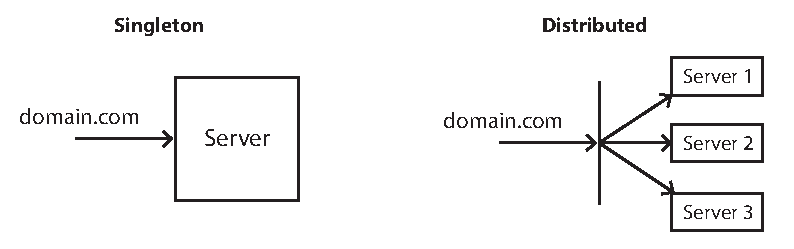
\includegraphics[width=\textwidth]{gfx/server_solutions.pdf}
    \caption{Illustration of a singleton and distributed server solution.}
    \label{fig:server_solutions}
\end{figure}

Distributed server solutions contain several servers possibly on several locations, meaning that DoS will be harder to perform, since there is no single point of failure.
However, this solution cannot ensure consistency and adds complexity.
The two solutions are graphically displayed in Figure~\ref{fig:server_solutions}.
A singleton solution has been chosen due to; consistency and simplicity.
This singleton solution will be denoted as Master or \deno{M}.

The application is required to handle communication with drones, as defined by \at{1} in Figure~\ref{tab:acceptance_tests1}.
In case of the communication being disabled, this might end up with a drone crash.
The technical limitations of antennas for digital wireless communication, sets a constraint for the availability of drones.
Assuming there exists no antenna to cover the physical area of our problem domain, it is necessary to have a distributed antenna setup in order to cover the whole physical area of the problem domain.
This leads to the structure shown in Figure~\ref{fig:antenna_structure}.

\begin{figure}[htb]
    \centering
    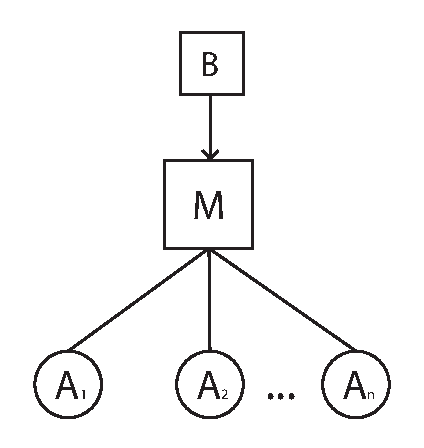
\includegraphics[width=0.5\textwidth]{gfx/antenna_structure.pdf}
    \caption{Antenna structure.}
    \label{fig:antenna_structure}
\end{figure}

If all \deno{B}'s communication with the drones goes through \deno{M}, this would create a single point of failure.
This means that, if \deno{M} crashes at any point, all communication with the drones will be disabled.
Providing the antennas with processing power and opportunity to communicate directly with \deno{B} would solve this issue.
If an antenna crashes only the drones connected to that antenna would be disconnected, leaving the drones connected to other antennas untouched.
This could be achieved by distributing some of the communication from \deno{M}.
This is solved by combining the antennas with distributed processing units, which will be denoted as Slaves or \deno{S}, as shown in Figure~\ref{fig:slave_structure}.

As \deno{S} has a dynamic network position relative to \deno{M}, this enforces that \deno{B} is not able to communicate directly with \deno{S} before getting network information about \deno{S} from \deno{M}. This communication is illustrated by a dashed line in Figure~\ref{fig:slave_structure}.

\begin{figure}[htb]
    \centering
    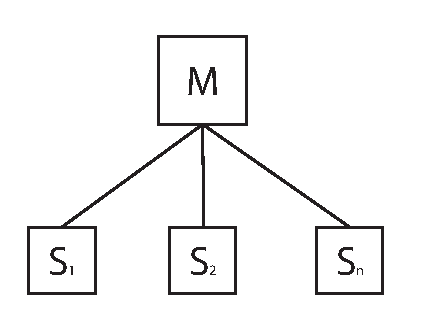
\includegraphics[width=0.5\textwidth]{gfx/slave_structure.pdf}
    \caption{Slave structure.}
    \label{fig:slave_structure}
\end{figure}

The acceptance tests, e.g. 17, 24, 25 in Figure~\ref{tab:acceptance_tests2}, enforces a constraint that requires \deno{M} to be able to store data based of the interaction of the user.
As requests can happen asynchronously, this makes it ideal to use a database denoted \deno{DB}, due to its transaction system in order to ensure no data loss.

The response output of \deno{M} needs to be dynamic based on the user, e.g. Acceptance test 2 in Figure~\ref{tab:acceptance_tests1}, which requires \deno{M} to be capable of processing data and store it in the database.
The processing unit that creates the dynamic response will be denoted \deno{W}.
The communication with the drones are handled by another processing unit, denoted \deno{D}.
If \deno{W} were to handle requests from \deno{S} and \deno{B}, this would increase the load on \deno{W}.
By creating multiple request handlers, it is possible to have a process for each. \deno{W}, \deno{DB}, and \deno{S} are processes, seen in Figure~\ref{fig:daemon_structure}, which improves resource management.
The resource management could be to constrain processing power for each process, or distribute the processes on individual machines.

\begin{figure}[htb]
    \centering
    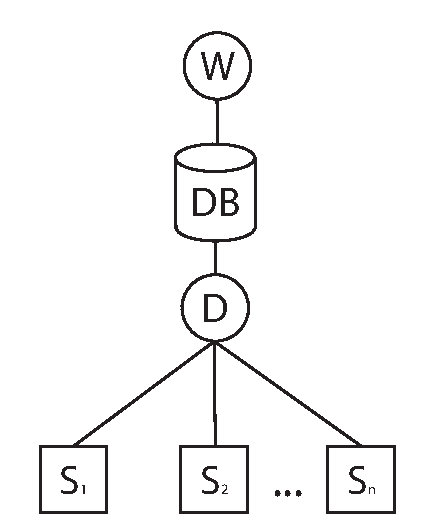
\includegraphics[width=0.5\textwidth]{gfx/daemon_structure.pdf}
    \caption{Daemon structure.}
    \label{fig:daemon_structure}
\end{figure}

% The architecture of \projectname{} differs from other web applications due to the fact that there exists two different type of servers.
% The architecture can be seen in figure~\ref{fig:system_architecture}.
% The server where the web application is running is called Master denoted M.
% For each drone in the system there is a Slave denoted S.
% On both M and S there exists daemons which is responsible for different tasks, however there is some similarity in the tasks they perform.
% These tasks can happen at anytime therefore the program needs to be running at anytime. These daemons are denoted D.
% Each user have a browser they view the application through this is denoted B.
% It is M's responsibility to communicate with every S in the system.
% S is responsible for all communication with the drone it is parred with.

% When a user wants to interact with a drone in the system a session key is needed.
% Such a session key is generated by S and then given to B through M.
% When both B and S have the same session key it is possible for them to communicate without M.
% This ensures that M does not become a bottleneck for controlling and streaming from drones and it reduces latency.
% When a new drone is added it is controlled by its S. This ensures that the system can scaled out and not have to scale up.
% Scale out means using more than one server where scale up means adding more processors, ram etc. to the server so it can handle more by itself.
% M does not handle commands and streaming, and every drone in the system have their own S.
% This makes the application architecture scalable because it removes bottlenecks from both M and S's.

% \begin{figure}[htb]
%     \centering
%     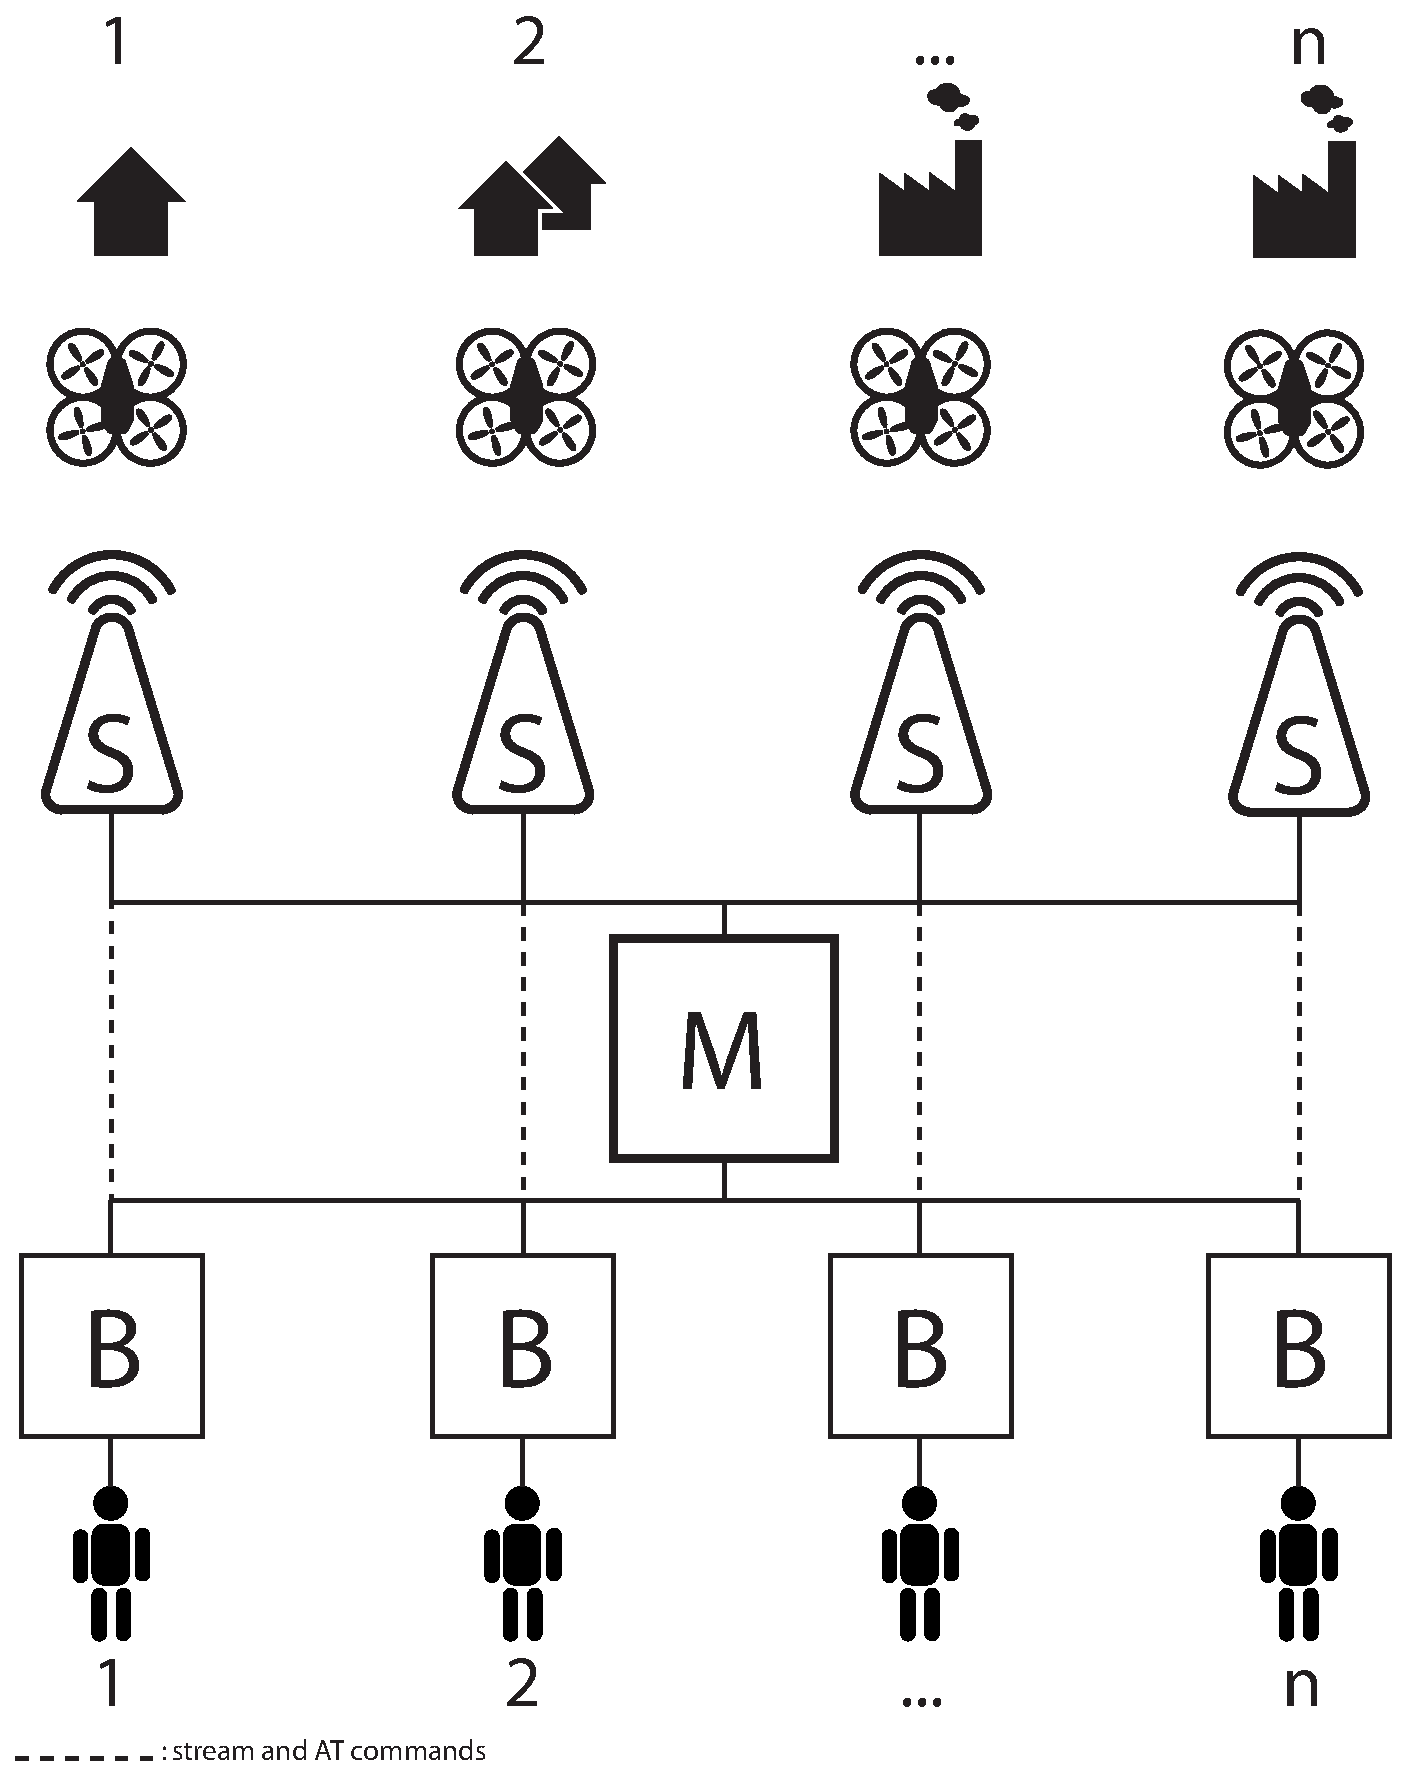
\includegraphics[width=\textwidth]{gfx/system_architecture.pdf}
%     \caption{System architecture of \projectname{}}
%     \label{fig:system_architecture}
% \end{figure}

% The system only uses one M. This can also be seen the bottleneck of the system.
% If M crashes all S's and B's will have to wait for M to come back up.
% One alternative could be running with more M's and in that way scale out.

% There is always one S for each drone connected to the system.
% In this way the system is scaled out.
% This ensures that any S is not likely to become a bottleneck.
% This was done because the drone uses wireless network which is short ranged and the drone is the host which means that the server needs one wireless connection for each drone it have to transmit to.
% One alternative could be only running with one S at each company and just scale it up.
% The problem with this is the server will need a wireless connection for each drone it have to control and it have to be in range.

% Daemon is a background process on a Linux system.
% Daemons are used when it is needed that a process is running at all times.
% In \projectname{} there are both the session key system which both resides on M and S and a policy file system for Adobe Flash on S.
% Both of these processes needs to be running at all times for the user to interact with the drone on S.
\section{Functionality distribution}\label{sec:functionality_distrubution}
% Hvilke funktionaliteter skal dækkes?
% Hvilke instancer dækker hvad?
% Hvorfor gør de det?

The functionality of the system can be derived from the acceptance tests.
This section will cover what instances are responsible for each functionality.

The need for storing data is derived from \at{1}, as previously described this is handled by the database \deno{DB}, which is a part of \deno{M}.
\at{2} sets the need for a dynamic response to \deno{B}, which requires processing of the stored data.
This processing is handled by Web or \deno{W} as the structure contains a singleton server solution.

Knowing that \deno{S} has a dynamic location relative to \deno{M}, this requires \deno{S} to send a signal to the daemon or \deno{D} in order for \deno{M} to get the location of \deno{S} on the network.
\deno{D} is then responsible for being able to receive incoming signals from \deno{S}.

Displaying video is required of \deno{B} by \at{3}.
The video displayed by \deno{B} is a stream, which requires that \deno{S} sends out a video stream.
In order to control a drone, commands have to be provided to the drone, as required by \at{3}.
\deno{S} is responsible for being able to receive commands and have the drone execute the given command.
\at{29} enforces security of the command handler.
\deno{S} is the only instance with a direct link to the drone, this makes \deno{S} responsible for the command handler's security.

% While Section~\ref{sec:application_structure} covered the overall structure of this application, this section will cover how the functionality is divided between the Master and the Slaves in the system. \\

% The Master is the users only way into the system.
% This access will always be via the users local web browser, where he sees the web system for \projectname{}.
% This web system and the database containing all informations about the system, drones, users etc. will be located on the Master.
% The Master is responsible for providing these services and coordinating the communication between the users and drones via the Slaves. \\

% A Slave is needed for every drone in the field, as the drones are not capable of long-distance communication.
% Therefore, in order to communicate with any drone, the communication must be channeled through its assigned Slave.
% This Slave is responsible for keeping contact with the drone and communicate directly with it via its API's.



\section{Communication network}\label{sec:communication_network}

Having functionality distributed across several instances sets the need for communication between the instances.
Based on Figure~\ref{fig:slave_structure}, which displays the dependency between \deno{B}, \deno{M}, and \deno{S} this leads to the diagram shown in Figure~\ref{fig:dataflow_diagrem}. \\


\begin{figure}[!h]
    \centering 
    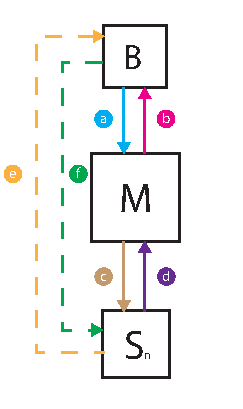
\includegraphics[width=0.5\textwidth]{gfx/dataflow_diagram.pdf}
    \caption{Dataflow diagram of \projectname{}}
    \label{fig:dataflow_diagrem}
\end{figure}


The arrows represent a connection, each connection represent dataflow in the direction of the arrow.
The type of data flowing in each connection and the reasons behind will be covered as each connection is discussed below. \\

Connection \deno{a} covers requests made by \deno{B}, which covers HTTP requests, which is a limit of web solutions that they must use the HTTP protocol.
HTTP requests enable the user to view the web application through his browser, and to send information.
In order to fulfill the request created by \deno{a}, a response is needed which the connection \deno{b} handles.
This connection covers the flow of the dynamic content created by \deno{M}, and static content such as: images, stylesheets, and multimedia objects.
Connection \deno{b} sends both the static and dynamic content back to \deno{B} to be displayed for the user. \\

The connection \deno{d} handles the signal described in Section~\ref{sec:functionality_distribution}.
This signal covers the initial communication between \deno{S} and \deno{M}. \deno{M} verifies the identity of \deno{S} by \deno{S} sending its own unique identifier.
This unique identifier is a string, which consist of X characters \fixme{How many chars?}.
All unique identifiers of each \deno{S} is known to \deno{M}.
This allows \deno{M} to determine the identity of each incoming signal. When \deno{M} receives a signal, and verify the identity of \deno{S}, the source location of the signal is stored in \deno{M} making \deno{M} able to know the location of \deno{S}. \\

Since requests from \deno{B} can happen asynchronously and from dynamic locations, it can create a problem that the identity of the connection made from \deno{S} to \deno{f} is not known. 
\at{28} sets the requirement of differentiating between incoming connections to \deno{S}.
If the communication described in connection \deno{e} and connection \deno{f} were running through \deno{M}, this would be no problem as security would be handled by the already existing sessions on \deno{M}.
The connections \deno{e} and \deno{f} are required to transport a large amount of data.
This data covers a video feed of the drone's video camera and commands for the drone.
This would increase the load on \deno{M}, which is not desired as \deno{M} is assumed to have a high load already.
However, since connection \deno{e} and connection \deno{f} are not running through \deno{M}, this leaves the problem of which \deno{B}, \deno{S} should listen to. \\

The solution chosen to solve this problem is to make \deno{S} create a randomly generated key (session key), that contains 40 characters and is unique relative to \deno{S} stored on \deno{S} itself.
When \deno{S} receives incoming commands, \deno{S} verifies whether or not the key received along with the command is equal to the one locally stored on \deno{S}.
If this is the case, \deno{S} classifies the received command as valid and performs the action.
The session key is delivered to \deno{B} from \deno{M}, as \deno{M} is able to verify the identity of \deno{B} through the session. \\

The connection \deno{c} covers requesting a session key by \deno{M}.
As \deno{M} has a static location, \deno{S} is able to verify the identity of \deno{M} based on its location.
Connection \deno{d} covers the response of the request received in \deno{c}, and \deno{M} is able to verify the identity of \deno{S} based on its location. \\

\begin{figure}[!h]
    \centering 
    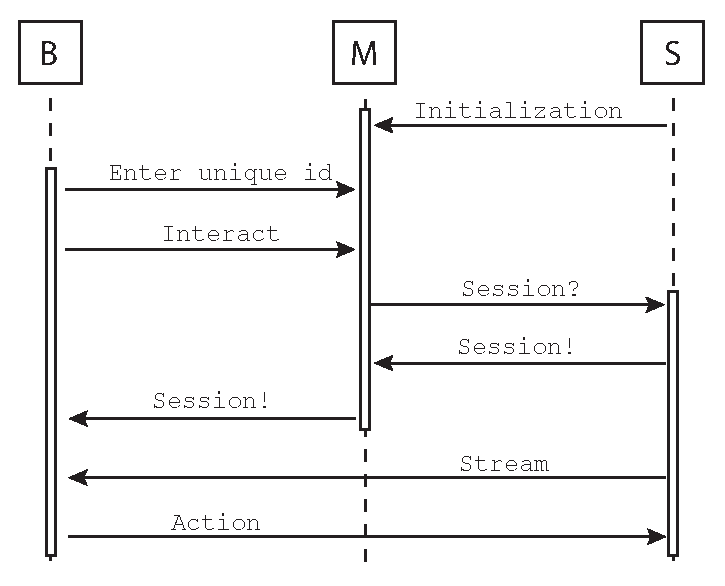
\includegraphics[width=\textwidth]{gfx/sequence_diagram.pdf}
    \caption{Sequence diagram of the communication network between \deno{B}, \deno{M}, and \deno{S}}
    \label{fig:sequence_diagram}
\end{figure}
\fxfatal{Check UML notation.}


The functionalities of the described connections, can only happen in a sequence as illustrated in Figure~\ref{fig:sequence_diagram}.
Each message in the sequence diagram can be done multiple times, however above messages are enforced to be performed atleast once in order for the given message to be performed. \\


% The communication network is crucial for \projectname{} to work.
% When designing a scalable communication network it is important to choose the right structure.
% There are different ways when designing such a network but identical for them all is that they need to support the structure of \deno{M}, \deno{S} and \deno{B} described in section~\ref{sec:application_structure}.

% One solution is to make a structure where \deno{M}, \deno{S} and \deno{B} talk to each other with a level of security. 
% The security aspect would be implemented with a form of session key. 
% This key would be used to determine if a session between a \deno{B} and a \deno{S} is valid.
% Another solution is to provide no security aspect and let it be up to the users and / or company to keep drones safe from intruders.
% This would lessen the communication between \deno{B}, \deno{M} and \deno{S}.  
% It would also decrease the load on \deno{M} and \deno{S}'s database. 
% On the down side the system could be considered not safe because it would be possible to tamper with the drones.
% As this is a system where it is important that the integrity is high, evidence is not tampered with, and where the outcome of an unauthorized user controller a drone could be devastating, it is important to deliver some form of security.



% This lead to a solution where sessions is designed to keep the integrity and secure evidence as seen in figure~\ref{fig:sequence_diagram}. 
% As seen in the figure there is designed a level of security because of the sessions.
% It is not possible for a \deno{B} to interact with a drone without having a session with a drones \deno{S}.

% When a drone is purchased a \deno{S} is setup at the location where the drone is going to operate.
% The \deno{S} sends an initializing message to \deno{M}, informing \deno{M} that a new drone has entered the system.
% \deno{M} adds the drone with the IP and location of the \deno{S}, along with the drone's unique identifier.
% If \deno{M} receives an initializing message from a \deno{S} with a drone identifier that is already in the system, it will destroy any session that correlates with that drone.
% The sessions is destroyed because if one or more sessions are granted and \deno{S} sends its initializing message it is safe to assume that \deno{S} either disconnected or crashed and all sessions keys are invalid.
% Furthermore if the IP of \deno{S} differs from the IP \deno{M} holds in its database it will be updated.

% If a user tries to interact with a drone the system behaves differently.
% A session key will be made on a \deno{S}, this key will be send to \deno{M} and giving to \deno{B}. If this session key is valid it is possible for the user to communicate directly with \deno{S} without \deno{M}.

% \begin{figure}[!h]
%     \centering 
%     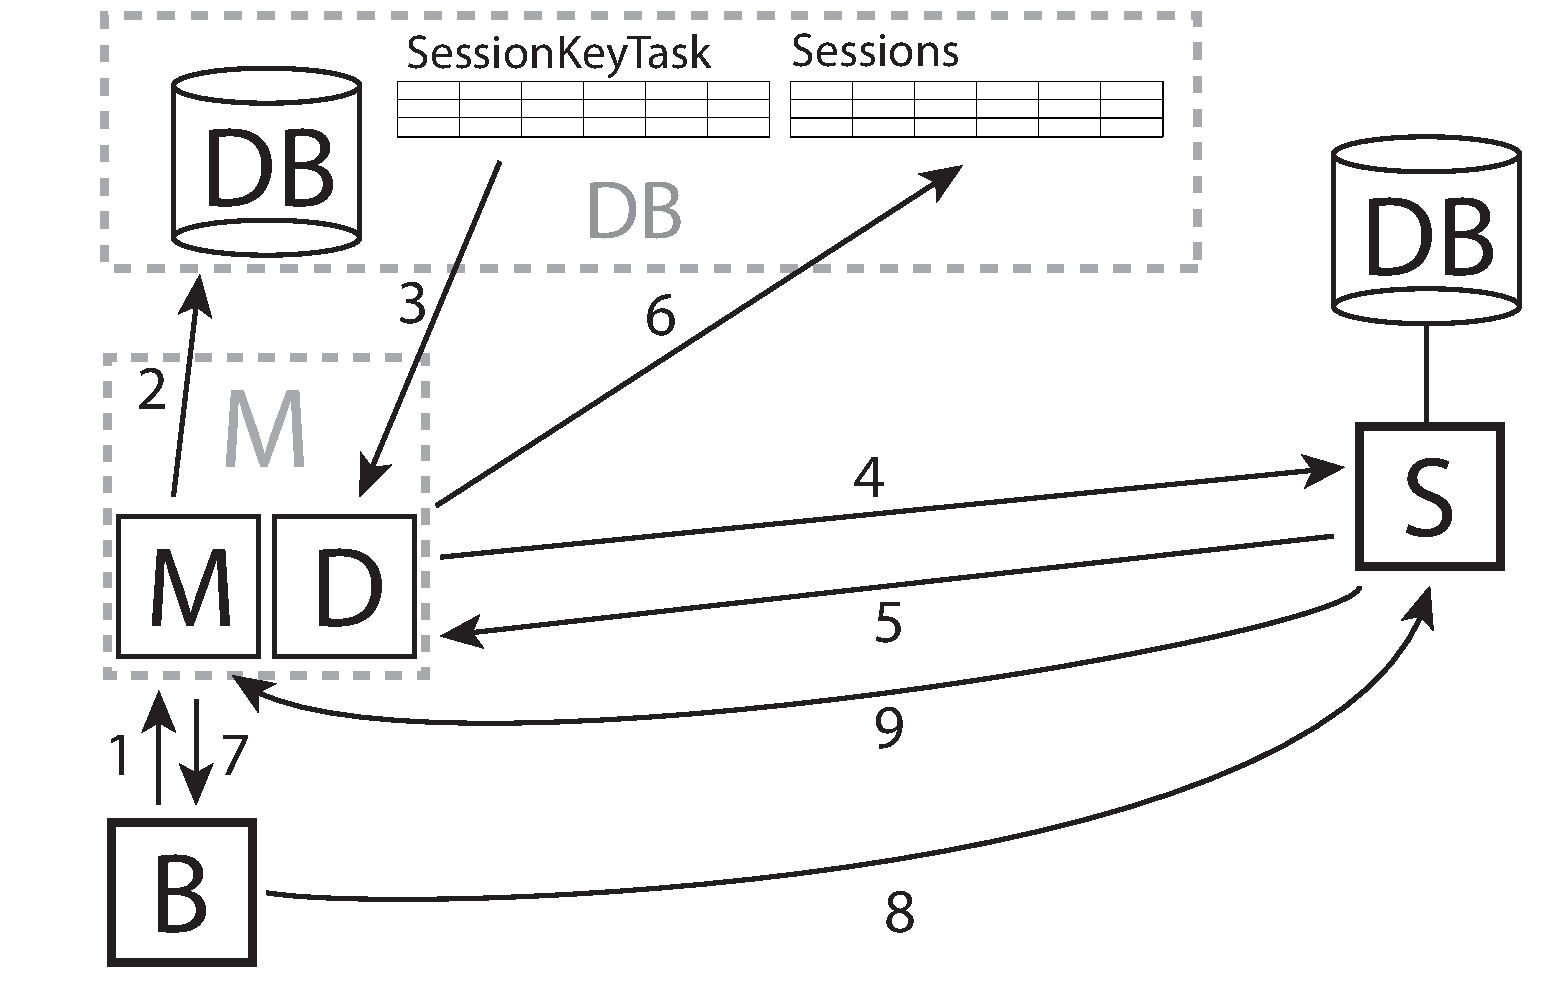
\includegraphics[width=\textwidth]{gfx/sessionkey_communication.pdf}
%     \caption{Session key communication between \deno{B}, \deno{M}, and \deno{S}}
%     \label{fig:sessionkey_communication}
% \end{figure}

% This behavior can be seen in figure~\ref{fig:sessionkey_communication}. 

% Session keys have been designed for security reasons.
% Firstly they were designed to ensure that only one user at a time can control a drone.
% Secondly it ensured that unauthorized users do not have the possibility of controlling a drone.

% \begin{enumerate}
% 	\item Request send from \deno{B} to \deno{M} about getting a session key to interact with a drone.
% 	\item \deno{M} inserts this request in its database table called SessionKeyTask.
% 	\item \deno{D} scans the database table SessionKeyTask, when it sees a new entry it select it and then deletes it from the table.
% 	\item \deno{D} requests a session key from \deno{S} parred with the drone the user wants to interact with.
% 	\item \deno{S} makes a random generated string with uppercase, lowercase letters and number. This string is used as the session key. \deno{S} updates its database with this session key and then sends it back to \deno{D} on \deno{M}.
% 	\item \deno{D} inserts the newly received session key into the session table of \deno{M}.
% 	\item \deno{M} then contacts \deno{B} with the session key.
% 	\item \deno{B} uses this session key to access \deno{S} and through it interact with the drone.
% 	\item A Timeout happens if \deno{B} and \deno{S} does not communicate for 10 seconds.
% \end{enumerate}

% Communication between the servers in the system is crucial. 
% Therefore it is important design a method or a set of methods handling the communication between them. 
% One method could be to make a service which handles all these requests on each server.
% The problem however is that using a single service might create a bottleneck.
% An alternative solution is to make a service for each communication level.
% One service that handles sessions, a service that handles control commands, and a service that handles initial messages from \deno{S} see section~\ref{sec:application_structure}.\fxfatal{Den her paragraf er uspecifik}

% This lead to a solution where the different actors in the system delivered and / or depended on services.

% The interface of the communication network can be seen in figure~\ref{fig:communication_network}.

% The communication network of \projectname{} uses four different ports for providing its services:

% \begin{itemize}
% 	\item Port A - service port for sending and receiving drone control commands.
% 	\item Port B - service port for receiving and sending initial messages.
% 	\item Port C - service port for sending and receiving session information including session keys.
% 	\item Port Web - service port for sending and receiving web specific information.
% \end{itemize}

% \begin{figure}[!h]
%     \centering 
%     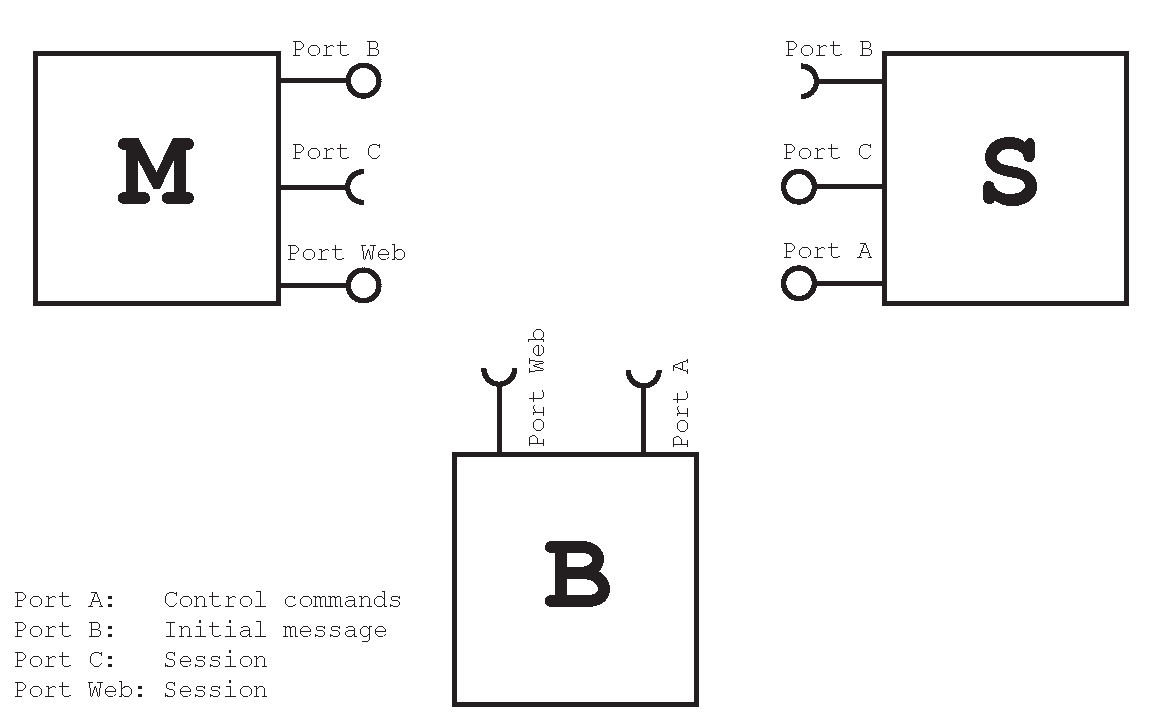
\includegraphics[width=\textwidth]{gfx/communication_network.pdf}
%     \caption{Communication network between \deno{B}, \deno{M}, and \deno{S}}
%     \label{fig:communication_network}
% \end{figure}

% When designing a communication network it is also important to select the right technique for exchanging data between services.
% One of the more widely used techniques are Extensible Markup Language.
% Extensible Markup Language, or XML for short, is a markup language designed to easily mark up data.
% The markup that XML provides makes it possible to easily send and receive data.
% The Extensible in XML makes it possible to extent what data types XML can handle through the XML schema. \citep{simonstl}
% This gives XML a drawback because XML is designed to be extensible it also carries a lot of overhead when used to mark up data.

% \projectname{} needs to be scalable therefore it is important to use as little overhead when sending structured information.
% Otherwise there is a chance that this overhead creates a bottleneck within the network.

% JSON, or JavaScript Object Notation, is design for data interchange and to be human-readable.
% It have a simpler syntax than XML and is not build to be extensible, it is not even a markup language. 
% It is a structured way of exchanging data between sources. 
% This results in less overhead i.e. it costs less data for each piece of information. 
% JSON is also data orientated which makes it easier to map a JSON object directly to a object orientated structure.
% Douglas Crockford call JSON ``The Fat-Free Alternative to XML'' \citep{JSON}.

% Therefore JSON is the perfect format for data interchange between the different services in \projectname{}. There are lesser costs associated with JSON than XML and it is easier to map them into a object orientated language.
\section{Object Model}
\label{section:uml_notation}
\label{subsec:objects}

This section will cover the design choices behind the application's object model, derived from the use cases in Section~\ref{sec:use_cases}.
The UML object model diagram can be seen in Figure~\ref{fig:UML_class_diagram}, and is guided by the UML standard guide written in cooperation by several different software companies~\citep{UML_notation}.\\

The UML attribute notation in this report is:
\begin{itemize}
    \item PK attribute - means that the attribute is a primary key.
    \item FK attribute - means that the attribute is a foreign key.
    \item attribute : type - all attributes will have a type e.g. \verb+id : int+.
\end{itemize}

The system will contain the following objects: \deno{Affiliate Privilege}, \deno{Company}, \deno{Drone}, \deno{Privilege}, \deno{Role}, \deno{Session}, and \deno{User}.
The model of the objects and their relationships can be seen in Figure~\ref{fig:UML_class_diagram}.
Each object covered is represented in the object model diagram with its name in lowercase and pluralized, e.g. \deno{User} object $\rightarrow$ \deno{users}.
If an object's name consists of several words the spaces will be replaced by underscores, e.g. Session Key Task becomes session\_key\_tasks.
The relationships between objects can either be implicit with a line directly from one object to another, or explicit with a simple or rich relationship model between the two objects.
Simple relationship models are models without a PK.
They are represented in the model diagram with both objects in lowercase and pluralized, e.g. roles\_users.
Rich relationship models have a PK.
This kind of relationship model does not have a predetermined naming convention, therefore it can be anything as long as it does not collide with the other model names, e.g. user\_privileges.\\

\begin{figure}[htb]
    \centering
    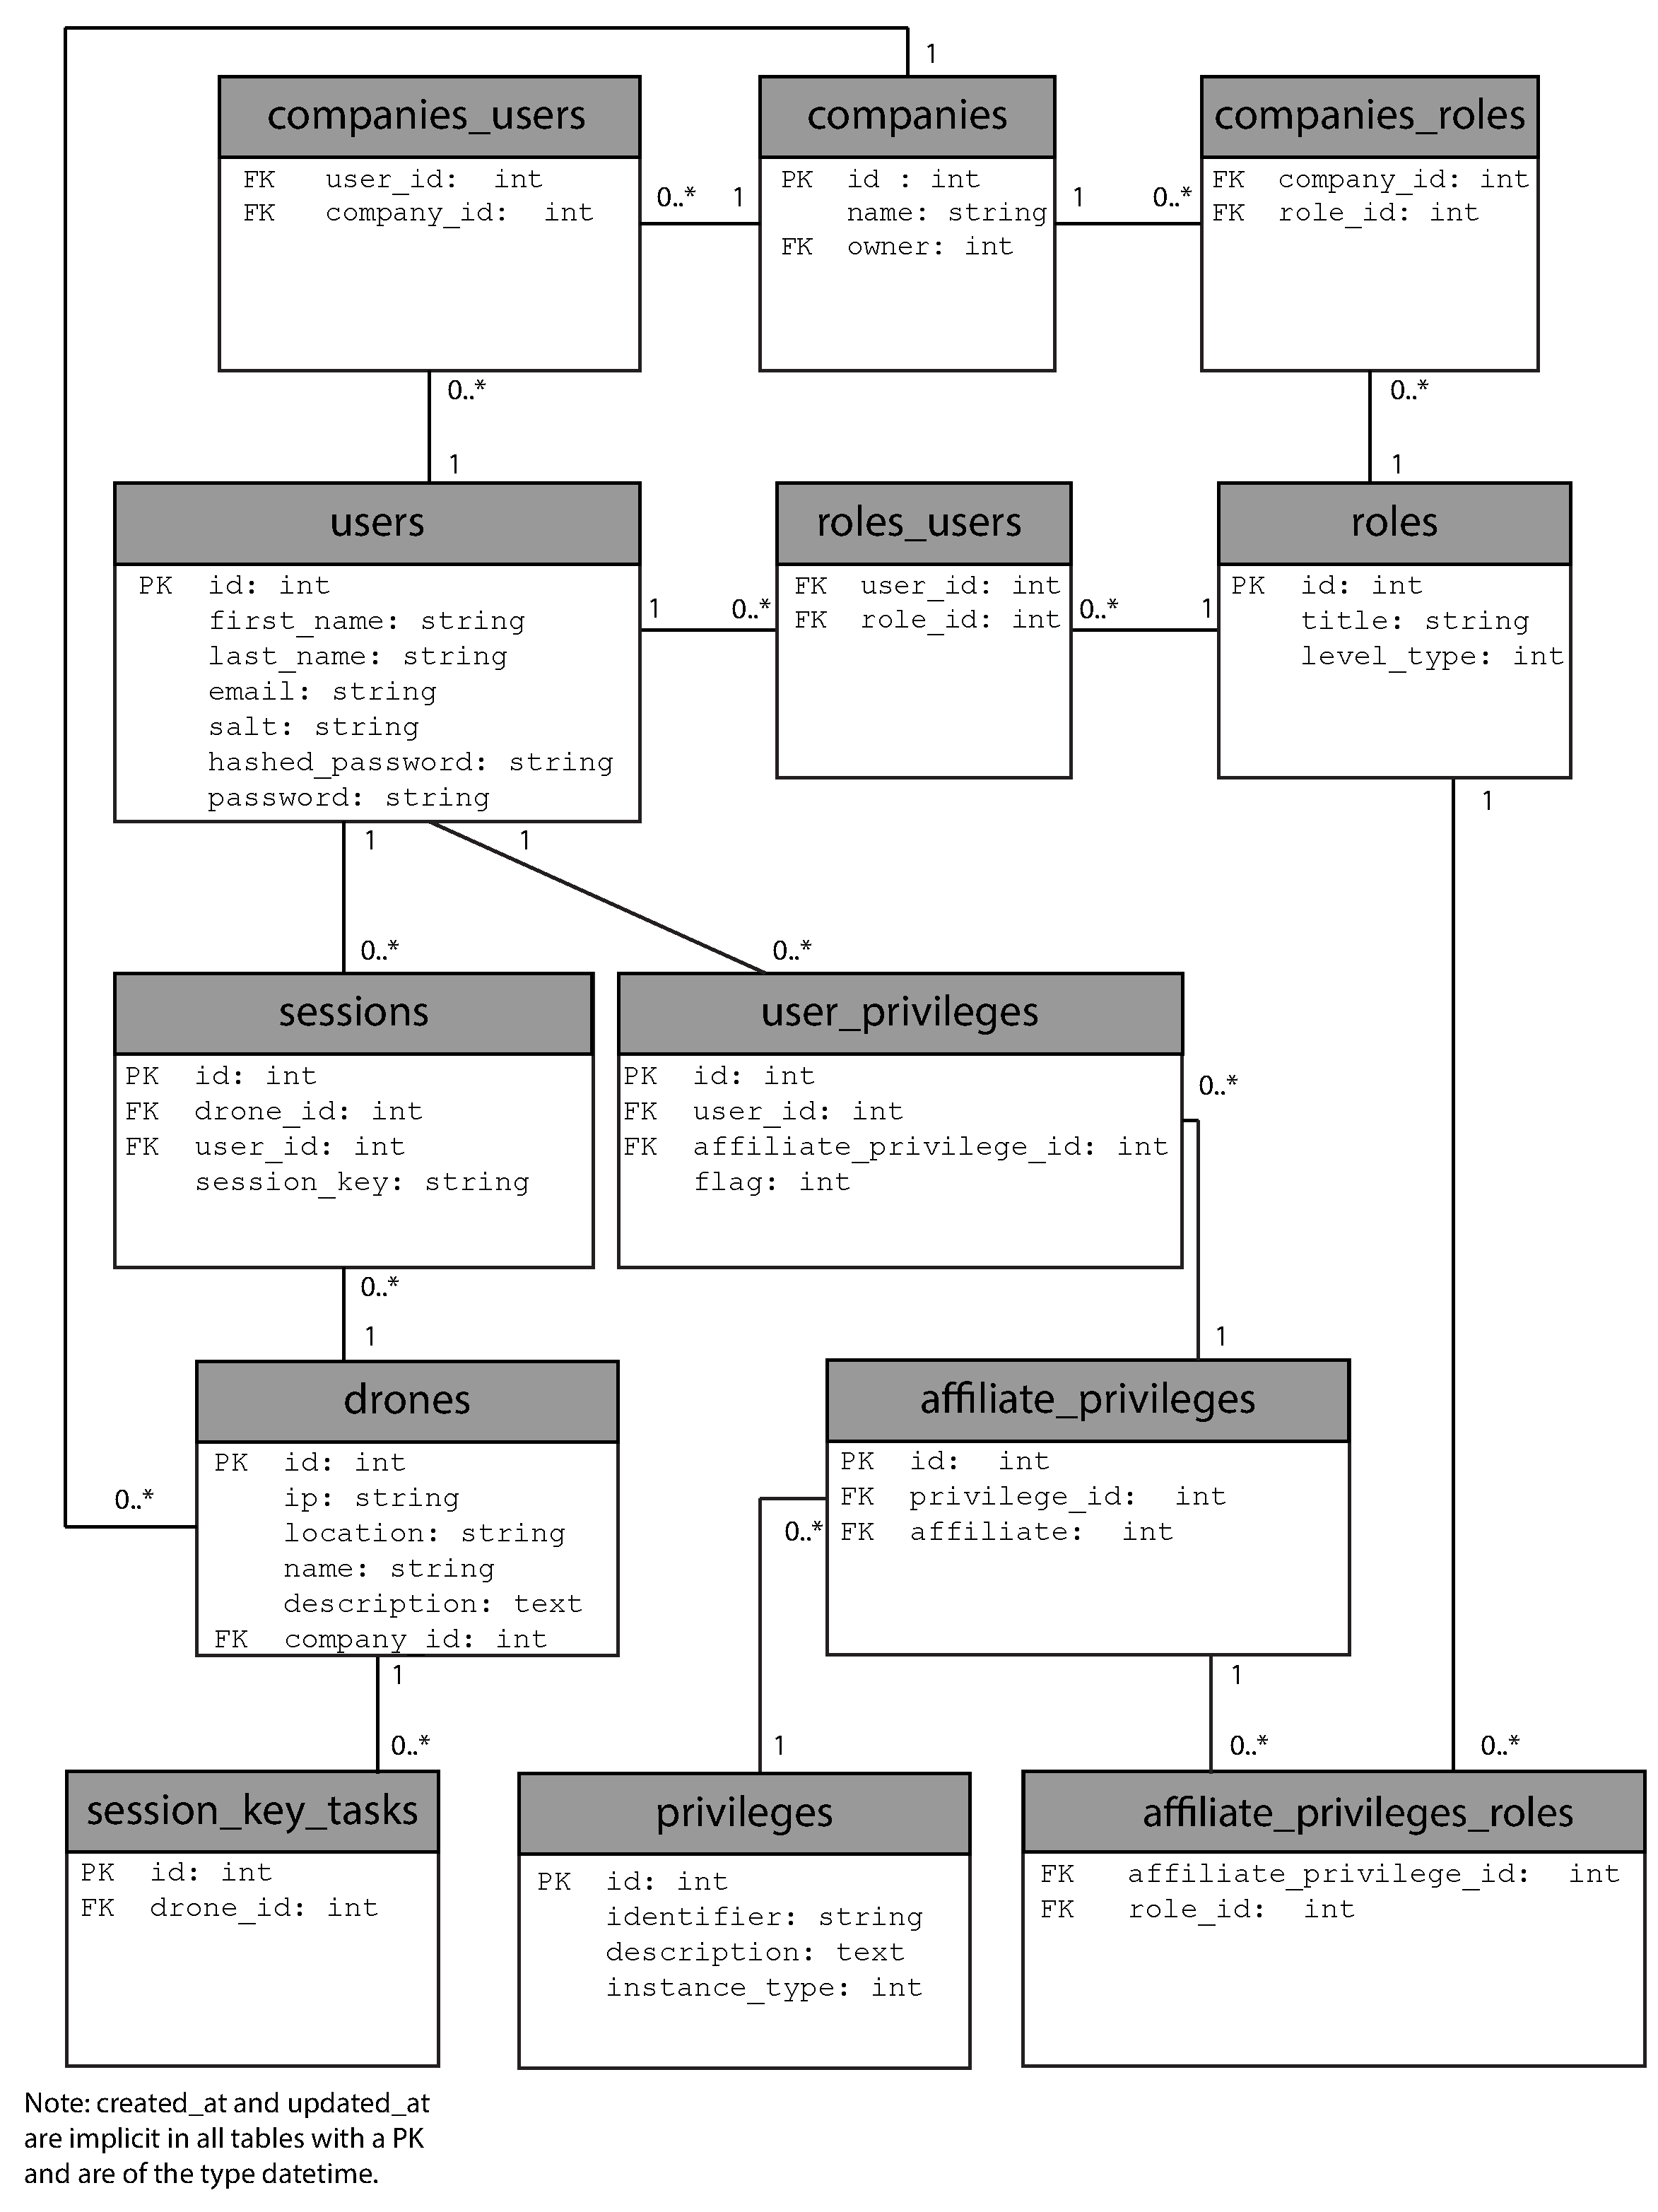
\includegraphics[width=0.95\textwidth]{gfx/UML_model.pdf}
    \caption{UML Class Diagram of \projectname{}}
    \label{fig:UML_class_diagram}
\end{figure}


\subsection{Objects}\fixme{Skal denne overskrift være der? Det burde ikke være nødvendigt at have den, men så skal teksten ændres lidt.}
Access to and actions of the system is restricted.
This restriction is based on the identity of user in the system.
An instance of the \deno{User} object represents a user to the system.
The \deno{User} object has the attributes \verb+email+ and \verb+password+, as seen in Figure~\ref{tab:user_object} in Appendix~\ref{app:objects}, these combined form the login credentials needed for a user to authenticate his identity towards the system. \\

The \verb+email+ is publicly available, which leaves the \verb+password+ to be protected in order for user to protect his identity in the system.
The \verb+password+ entered by the user is concatenated with a \verb+salt+ and hashed through a SHA-1 hashing algorithm to be stored in \verb+hashed_password+.
The hashing algorithm provides a way for storing the password without having its exact value, as this could leave to a security flaw.
Having access to passwords of users directly, e.g. through a hacker attack, would allow the hacker to login into the users account, which is unintended for the system.
When a salt is concatenated before hashing it makes it harder for the hacker to gain the original passwords, e.g. through a rainbow table~\cite{something}. \\

Having a distributed setup with multiple \deno{S}, each representing a \deno{Drone} object, means that the network locations of these need to be known in order to communicate.
The network location is stored in the \verb+ip+ field of the \deno{Drone} object, as shown in Figure~\ref{tab:drone_object} of Appendix~\ref{app:objects}.
The physical drone have a unique identifier known as \verb+name+, which makes the user able to identify a given drone. \\

The users of the system will be part of different companies, therefore there is a need for grouping users by a company.
The \deno{Company} object have an \verb+owner+, which is a reference to a \deno{User} object.
This is required for the system to know which user have access to all \deno{Affiliate Privilege} objects of the company. \\

An \deno{Affiliate Privilege} object references a \deno{Privilege}, and only when combined they form a unique key.
This key unlocks a certain functionality, meaning that if the user does not have a relation to the \deno{Affiliate Privilege} object, which represents the key, then the user is not able to unlock that functionality.
\deno{Role} objects give the possibility of grouping \deno{Privilege} objects together.
Each \deno{Company} have a related role which contains all privileges, of which the company have full control.
Full control gives the right for passing on a privilege, or disabling if the privilege is already granted.
\deno{Affiliate Privilege} objects have a field \verb+affiliate+ that links the privilege to an object of the type declared by the referenced \deno{Privilege} object's \verb+instance_type+ field. \\

The \deno{Session} object represents an active pilot connection between a user and a drone.
The \verb+session_key+ field provides a key that needs to be sent along with the commands.
The \deno{Session Key Task} object is an object used for \deno{D} and \deno{M} to communicate through \deno{DB}, as shown in Figure~\ref{fig:daemon_structure} in Section~\ref{sec:application_structure}. \\

In Section~\ref{sec:privileges} solutions for handling privileges were discussed.
From this discussion it was decided to model a system capable of handling all proposed solutions to fit scenarios of the users.
The \deno{User Privileges} relationship allows for connecting individual {Privilege} objects to a \deno{User} object.
This is could be either granting or revoking, i.e. exceptions, the privilege.
The \verb+flag+ field represents a value of either 1 or -1; 1 is regarded as granted, and -1 is regarded as revoked.


% \subsection{Relationships}
% The system is designed with flexibility and scalability in mind, and the structure of Roles and Privileges are what provides those features.
% As described before there are two ways that a User can be granted a specific Privilege.
% These are by 1) getting the Privilege granted directly via the \verb+User_Privileges+ table or 2) by being a member of a Role that via the \verb+Privileges_Roles+ table that has one or more Privileges granted.
% These will be explained in details in the following subsections.


% % Users and Privileges %
% An administrator can grant a specific Privilege directly to a user via the \verb+User_Privileges+ table.
% This Privilege is then affiliated with an object -- usually a Drone.
% The Privilege could also be a system functionality, however, as described in Section~\ref{sec:privileges}. \\

% This relationship is also used for exceptions.
% In an example where five Users: U1, U2, U3, U4 and U5 are a member of a Role: R1, we may have a situation where U2 is not suppose to have access to a given Privilege P1 in R1.
% Then a User-specific Privilege is granted to U2 on P1, but with the ``exception''-flag marked.
% This is equal to blacklisting U2 from using Privilege P1, providing the system with a lot of flexibility, as even though a group of Users are granted a number of Privileges via a role, User-specific exceptions can be added to this setting. \\


% % Roles and Privileges %
% As mentioned before -- the reason that Roles can be used to assign Privileges to a User, is to make both the administration and data structure of Users and Privileges as simple and efficient as possible.
% By allowing exceptions, full flexibility is still possible. \\

% This is how the relationship between Roles and Privileges works: \\

% An administrator creates a Role.
% Lets call this Role ``Control Drone \#4''.
% A number of Privileges are assigned to this Role.
% It could be the following:

% \begin{itemize}
%     \item Watch the video feed from a specific drone
%     \item Control the movement of a specific drone
% \end{itemize}

% Those Privileges are then linked to this Role and to the Drone this concerns. \\

% Roles can be assigned with affiliation to both Users and Companies.
% Say a user \verb+U1+ needs access to Drone \#4.
% User U1 then needs to either have the Privileges directly granted or be a member of the role ``Control Drone \#4''.


% % Privileges and granting of Privileges %
% Since it is possible to grant Privileges both directly to a User and via a Role, the same Privilege can be used in more than one context.
% Therefore the \verb+Affiliation_Privileges+ table exists.
% This table links the granting of a Privilege with the actual Privilege and defines on which Object the Privilege applies.
% The reason for having this table and not just link the two granting-tables \verb+User_Privileges+ and \verb+Privileges_Roles+ directly to the \verb+Privileges+ table, is that we try to avoid redundant data by having the data in the \verb+Privileges+ and \verb+Affiliation_Privileges+ table make up one instance of a privilege together.
% This is then granted to a User or a Role, who can then use the Privilege. \\

% The system is designed so that any User can grant a Privilege he already has already been granted to another User if he is permitted to.
% This is controlled via a ``re-grantable'' flag which is set in either the \verb+User_Privileges+ table or the \verb+Privileges_Roles+ table.
% By marking this flag as ``true'', the User or Users that via a Role is granted the Privilege in question, can via an interface in the system re-grant the Privilege to other Users in the same Company.


% %Note: Alle brugere kan videregrante et privilege hvis de har tilladelse til det. Det er et flag som sætes i user_privileges og privileges_roles, som tillader alle der har dette privilegie til at videregrante det. Husk at beskrive hvordan et privilege og et affiliation privilege til sammen giver et grant-able privilegie


% % Privileges and Drones %
% With \projectname{} in its current form, most Privileges that are granted will have an connected with a Drone.
% Privileges and its a affiliations are linked in the \verb+Affiliation_Privileges+ table.
% This is also where Drones are linked to any granted privilege. \\

% As described earlier, Drones are the current object-type implemented in the system.
% However, the structure and model of the system allows for later expansion, connection new objects such as stationary cameras or any other type of object to the system.
% The \verb+Affiliation_Privileges+ has a third field named \verb+object_id+.
% This field links the Privilege, the granting of it and the Object that this granting is valid for. \\

% An example could be linking Privilege P1, User U1 and Drone D1.
% Say P1 is the privilege for watching the video feed of a drone.
% Then the user U1 will have access to watch the video feed of Drone D1.


% % Drones and Companies %
% The \verb+Company_drones+ table defines a relationship between a Drone and a Company.

% The administrator of each Company defines the Roles in that Company.
% In doing so, he defines which Privileges that are granted in every Role.
% These Privileges are linked to a (Drone)-object.
% The system must make sure that any Company administrator cannot link a Privilege with a Object that is not within his control. \\

% This relationship defines which Drones are available to each Company.
% When a Company administrator adds new Roles (and hence Privileges), he is only able to associate it with Drones that are connected to the Company in question.

% **************************************************************************************************************
% A Classic Thesis Style
% An Homage to The Elements of Typographic Style
%
% Copyright (C) 2012 Andr\'e Miede http://www.miede.de
%
% If you like the style then I would appreciate a postcard. My address
% can be found in the file ClassicThesis.pdf. A collection of the
% postcards I received so far is available online at
% http://postcards.miede.de
%
% License:
% This program is free software; you can redistribute it and/or modify
% it under the terms of the GNU General Public License as published by
% the Free Software Foundation; either version 2 of the License, or
% (at your option) any later version.
%
% This program is distributed in the hope that it will be useful,
% but WITHOUT ANY WARRANTY; without even the implied warranty of
% MERCHANTABILITY or FITNESS FOR A PARTICULAR PURPOSE.  See the
% GNU General Public License for more details.
%
% You should have received a copy of the GNU General Public License
% along with this program; see the file COPYING.  If not, write to
% the Free Software Foundation, Inc., 59 Temple Place - Suite 330,
% Boston, MA 02111-1307, USA.
%
% **************************************************************************************************************
% Note:
%    * You must not use "u etc. in strings/commands that will be spaced out (use \"u or real umlauts instead)
%    * New enumeration (small caps): \begin{aenumerate} \end{aenumerate}
%    * For margin notes: \marginpar or \graffito{}
%    * Do not use bold fonts in this style, it is designed around them
%    * Use tables as in the examples
%    * See classicthesis-preamble.sty for useful commands
% **************************************************************************************************************
% To Do:
%		 * [high] Check this out: http://www.golatex.de/koma-script-warnung-in-verbindung-mit-listings-package-t2058.html
%    * [medium] mathbb in section-titles/chapter-titles => disappears somehow in headlines!!!
% **************************************************************************************************************
\documentclass[ twoside,openright,titlepage,numbers=noenddot,headinclude,%1headlines,% letterpaper a4paper
                footinclude=true,cleardoublepage=empty,abstractoff, % <--- obsolete, remove (todo)
                BCOR=5mm,paper=a4,fontsize=11pt,%11pt,a4paper,%
                ngerman,american,%
                ]{scrreprt}

%********************************************************************
% Note: Make all your adjustments in here
%*******************************************************
% ****************************************************************************************************
% classicthesis-config.tex
% formerly known as loadpackages.sty, classicthesis-ldpkg.sty, and classicthesis-preamble.sty
% Use it at the beginning of your ClassicThesis.tex, or as a LaTeX Preamble
% in your ClassicThesis.{tex,lyx} with \input{classicthesis-config}
% ****************************************************************************************************
% If you like the classicthesis, then I would appreciate a postcard.
% My address can be found in the file ClassicThesis.pdf. A collection
% of the postcards I received so far is available online at
% http://postcards.miede.de
% ****************************************************************************************************

% ****************************************************************************************************
% 1. Configure classicthesis for your needs here, e.g., remove "drafting" below
% in order to deactivate the time-stamp on the pages
% ****************************************************************************************************
\PassOptionsToPackage{eulerchapternumbers,listings,drafting,%
				 pdfspacing,%floatperchapter,%linedheaders,%
				 subfig,beramono,eulermath,parts}{classicthesis}
% ********************************************************************
% Available options for classicthesis.sty
% (see ClassicThesis.pdf for more information):
% drafting
% parts nochapters linedheaders
% eulerchapternumbers beramono eulermath pdfspacing minionprospacing
% tocaligned dottedtoc manychapters
% listings floatperchapter subfig
% ********************************************************************

% ********************************************************************
% Triggers for this config
% ********************************************************************
\usepackage{ifthen}
\newboolean{enable-backrefs} % enable backrefs in the bibliography
\setboolean{enable-backrefs}{false} % true false
% ****************************************************************************************************


% ****************************************************************************************************
% 2. Personal data and user ad-hoc commands
% ****************************************************************************************************
\newcommand{\myTitle}{LONE\xspace}
\newcommand{\mySubtitle}{Lone is Observation of Nondeterministic Environments\xspace}
%\newcommand{\myDegree}{Doktor-Ingenieur (Dr.-Ing.)\xspace}
\newcommand{\myName}{SW701E12\xspace}
\newcommand{\myProf}{Put name here\xspace}
\newcommand{\myOtherProf}{Put name here\xspace}
\newcommand{\mySupervisor}{Put name here\xspace}
\newcommand{\myFaculty}{Put data here\xspace}
\newcommand{\myDepartment}{Put data here\xspace}
\newcommand{\myUni}{Aalborg University\xspace}
\newcommand{\myLocation}{Aalborg\xspace}
\newcommand{\myTime}{December 2012\xspace}
\newcommand{\myVersion}{version 4.1\xspace}
\newcommand{\projectname}{<projectname>}

% ********************************************************************
% Setup, finetuning, and useful commands
% ********************************************************************
\newcounter{dummy} % necessary for correct hyperlinks (to index, bib, etc.)
\newlength{\abcd} % for ab..z string length calculation
\providecommand{\mLyX}{L\kern-.1667em\lower.25em\hbox{Y}\kern-.125emX\@}
\newcommand{\ie}{i.\,e.}
\newcommand{\Ie}{I.\,e.}
\newcommand{\eg}{e.\,g.}
\newcommand{\Eg}{E.\,g.}
% ****************************************************************************************************


% ****************************************************************************************************
% 3. Loading some handy packages
% ****************************************************************************************************
% ********************************************************************
% Packages with options that might require adjustments
% ********************************************************************
\PassOptionsToPackage{latin9}{inputenc}	% latin9 (ISO-8859-9) = latin1+"Euro sign"
 \usepackage{inputenc}

%\PassOptionsToPackage{ngerman,american}{babel}   % change this to your language(s)
% Spanish languages need extra options in order to work with this template
%\PassOptionsToPackage{spanish,es-lcroman}{babel}
 \usepackage{babel}

\PassOptionsToPackage{square,numbers}{natbib}
 \usepackage{natbib}

\PassOptionsToPackage{fleqn}{amsmath}		% math environments and more by the AMS
 \usepackage{amsmath}

% ********************************************************************
% General useful packages
% ********************************************************************
\PassOptionsToPackage{T1}{fontenc} % T2A for cyrillics
	\usepackage{fontenc}
\usepackage{textcomp} % fix warning with missing font shapes
\usepackage{scrhack} % fix warnings when using KOMA with listings package
\usepackage{xspace} % to get the spacing after macros right
\usepackage{mparhack} % get marginpar right
\usepackage{fixltx2e} % fixes some LaTeX stuff
\PassOptionsToPackage{printonlyused,smaller}{acronym}
	\usepackage{acronym} % nice macros for handling all acronyms in the thesis
%\renewcommand*{\acsfont}[1]{\textssc{#1}} % for MinionPro
\renewcommand{\bflabel}[1]{{#1}\hfill} % fix the list of acronyms
\usepackage[footnote,draft,english,silent,nomargin]{fixme}  % final instead of draft produces errors at
                                                            % compile time
                                                            
%Bjarke HS stuff
\newcommand{\todo}[1]{\fxnote{#1}}
\newcommand{\todoi}[1]{\fxfatal{#1}}
\newcommand{\todoI}[1]{\todoi{#1}}

%Rasmus stuff
\newcommand{\figref}[1]{\figurename~\ref{#1}}

% ****************************************************************************************************


% ****************************************************************************************************
% 4. Setup floats: tables, (sub)figures, and captions
% ****************************************************************************************************
\usepackage{tabularx} % better tables
	\setlength{\extrarowheight}{3pt} % increase table row height
\newcommand{\tableheadline}[1]{\multicolumn{1}{c}{\spacedlowsmallcaps{#1}}}
\newcommand{\myfloatalign}{\centering} % to be used with each float for alignment
\usepackage{caption}
\captionsetup{format=hang,font=small}
\usepackage{subfig}
% ****************************************************************************************************


% ****************************************************************************************************
% 5. Setup code listings
% ****************************************************************************************************
\usepackage{listings}
%\lstset{emph={trueIndex,root},emphstyle=\color{BlueViolet}}%\underbar} % for special keywords
\lstset{language=[LaTeX]Tex,%C++,
    keywordstyle=\color{RoyalBlue},%\bfseries,
    basicstyle=\small\ttfamily,
    %identifierstyle=\color{NavyBlue},
    commentstyle=\color{Green}\ttfamily,
    stringstyle=\rmfamily,
    numbers=none,%left,%
    numberstyle=\scriptsize,%\tiny
    stepnumber=5,
    numbersep=8pt,
    showstringspaces=false,
    breaklines=true,
    frameround=ftff,
    frame=single,
    belowcaptionskip=.75\baselineskip
    %frame=L
}
% ****************************************************************************************************


% ****************************************************************************************************
% 6. PDFLaTeX, hyperreferences and citation backreferences
% ****************************************************************************************************
% ********************************************************************
% Using PDFLaTeX
% ********************************************************************
\PassOptionsToPackage{pdftex,hyperfootnotes=false,pdfpagelabels}{hyperref}
	\usepackage{hyperref}  % backref linktocpage pagebackref
\pdfcompresslevel=9
\pdfadjustspacing=1
\PassOptionsToPackage{pdftex}{graphicx}
	\usepackage{graphicx}

% ********************************************************************
% Setup the style of the backrefs from the bibliography
% (translate the options to any language you use)
% ********************************************************************
\newcommand{\backrefnotcitedstring}{\relax}%(Not cited.)
\newcommand{\backrefcitedsinglestring}[1]{(Cited on page~#1.)}
\newcommand{\backrefcitedmultistring}[1]{(Cited on pages~#1.)}
\ifthenelse{\boolean{enable-backrefs}}%
{%
		\PassOptionsToPackage{hyperpageref}{backref}
		\usepackage{backref} % to be loaded after hyperref package
		   \renewcommand{\backreftwosep}{ and~} % separate 2 pages
		   \renewcommand{\backreflastsep}{, and~} % separate last of longer list
		   \renewcommand*{\backref}[1]{}  % disable standard
		   \renewcommand*{\backrefalt}[4]{% detailed backref
		      \ifcase #1 %
		         \backrefnotcitedstring%
		      \or%
		         \backrefcitedsinglestring{#2}%
		      \else%
		         \backrefcitedmultistring{#2}%
		      \fi}%
}{\relax}

% ********************************************************************
% Hyperreferences
% ********************************************************************
\hypersetup{%
    %draft,	% = no hyperlinking at all (useful in b/w printouts)
    colorlinks=true, linktocpage=true, pdfstartpage=3, pdfstartview=FitV,%
    % uncomment the following line if you want to have black links (e.g., for printing)
    %colorlinks=false, linktocpage=false, pdfborder={0 0 0}, pdfstartpage=3, pdfstartview=FitV,%
    breaklinks=true, pdfpagemode=UseNone, pageanchor=true, pdfpagemode=UseOutlines,%
    plainpages=false, bookmarksnumbered, bookmarksopen=true, bookmarksopenlevel=1,%
    hypertexnames=true, pdfhighlight=/O,%nesting=true,%frenchlinks,%
    urlcolor=webbrown, linkcolor=RoyalBlue, citecolor=webgreen, %pagecolor=RoyalBlue,%
    %urlcolor=Black, linkcolor=Black, citecolor=Black, %pagecolor=Black,%
    pdftitle={\myTitle},%
    pdfauthor={\textcopyright\ \myName, \myUni, \myFaculty},%
    pdfsubject={},%
    pdfkeywords={},%
    pdfcreator={pdfLaTeX},%
    pdfproducer={LaTeX with hyperref and classicthesis}%
}

% ********************************************************************
% Setup autoreferences
% ********************************************************************
% There are some issues regarding autorefnames
% http://www.ureader.de/msg/136221647.aspx
% http://www.tex.ac.uk/cgi-bin/texfaq2html?label=latexwords
% you have to redefine the makros for the
% language you use, e.g., american, ngerman
% (as chosen when loading babel/AtBeginDocument)
% ********************************************************************
\makeatletter
\@ifpackageloaded{babel}%
    {%
       \addto\extrasamerican{%
					\renewcommand*{\figureautorefname}{Figure}%
					\renewcommand*{\tableautorefname}{Table}%
					\renewcommand*{\partautorefname}{Part}%
					\renewcommand*{\chapterautorefname}{Chapter}%
					\renewcommand*{\sectionautorefname}{Section}%
					\renewcommand*{\subsectionautorefname}{Section}%
					\renewcommand*{\subsubsectionautorefname}{Section}%
				}%
       \addto\extrasngerman{%
					\renewcommand*{\paragraphautorefname}{Absatz}%
					\renewcommand*{\subparagraphautorefname}{Unterabsatz}%
					\renewcommand*{\footnoteautorefname}{Fu\"snote}%
					\renewcommand*{\FancyVerbLineautorefname}{Zeile}%
					\renewcommand*{\theoremautorefname}{Theorem}%
					\renewcommand*{\appendixautorefname}{Anhang}%
					\renewcommand*{\equationautorefname}{Gleichung}%
					\renewcommand*{\itemautorefname}{Punkt}%
				}%
			% Fix to getting autorefs for subfigures right (thanks to Belinda Vogt for changing the definition)
			\providecommand{\subfigureautorefname}{\figureautorefname}%
    }{\relax}
\makeatother


% ****************************************************************************************************
% 7. Last calls before the bar closes
% ****************************************************************************************************
% ********************************************************************
% Development Stuff
% ********************************************************************
\listfiles
%\PassOptionsToPackage{l2tabu,orthodox,abort}{nag}
%	\usepackage{nag}
%\PassOptionsToPackage{warning, all}{onlyamsmath}
%	\usepackage{onlyamsmath}

% ********************************************************************
% Last, but not least...
% ********************************************************************
\usepackage{classicthesis}
% ****************************************************************************************************


% ****************************************************************************************************
% 8. Further adjustments (experimental)
% ****************************************************************************************************
% ********************************************************************
% Changing the text area
% ********************************************************************
%\linespread{1.05} % a bit more for Palatino
%\areaset[current]{312pt}{761pt} % 686 (factor 2.2) + 33 head + 42 head \the\footskip
%\setlength{\marginparwidth}{7em}%
%\setlength{\marginparsep}{2em}%

% ********************************************************************
% Using different fonts
% ********************************************************************
%\usepackage[oldstylenums]{kpfonts} % oldstyle notextcomp
%\usepackage[osf]{libertine}
%\usepackage{hfoldsty} % Computer Modern with osf
%\usepackage[light,condensed,math]{iwona}
%\renewcommand{\sfdefault}{iwona}
%\usepackage{lmodern} % <-- no osf support :-(
%\usepackage[urw-garamond]{mathdesign} <-- no osf support :-(
% ****************************************************************************************************


%********************************************************************
% Hyphenation
%*******************************************************
%\hyphenation{put special hyphenation here}

% ********************************************************************
% GO!GO!GO! MOVE IT!
%*******************************************************
\begin{document}
\frenchspacing
\raggedbottom
\selectlanguage{american} % american ngerman
%\renewcommand*{\bibname}{new name}
%\setbibpreamble{}
\pagenumbering{roman}
\pagestyle{plain}
%********************************************************************
% Frontmatter
%*******************************************************
%%*******************************************************
% Little Dirty Titlepage
%*******************************************************
\thispagestyle{empty}
%\pdfbookmark[1]{Titel}{title}
%*******************************************************
\begin{center}
    \spacedlowsmallcaps{\myName} \\ \medskip                        

    \begingroup
        \color{Maroon}\spacedallcaps{\myTitle}
    \endgroup
\end{center}        

%*******************************************************
% Titlepage
%*******************************************************
\begin{titlepage}
	% if you want the titlepage to be centered, uncomment and fine-tune the line below (KOMA classes environment)
	\begin{addmargin}[-1cm]{-3cm}
    \begin{center}
        \large  

        \hfill

        \vfill

        \begingroup
            \color{Maroon}\spacedallcaps{\myTitle} \\ \bigskip
        \endgroup

        \vfill

        %\myDegree \\
        %\myDepartment \\                            
        %\myFaculty \\
        %\myUni \\ \bigskip

        \myTime\ -- \myVersion

        \vfill                      

    \end{center}  
  \end{addmargin}       
\end{titlepage}   
\thispagestyle{empty}

\hfill

\vfill

\noindent\myName: \textit{\myTitle,} \mySubtitle, %\myDegree, 
\textcopyright\ \myTime

%\bigskip
%
%\noindent\spacedlowsmallcaps{Supervisors}: \\
%\myProf \\
%\myOtherProf \\ 
%\mySupervisor
%
%\medskip
%
%\noindent\spacedlowsmallcaps{Location}: \\
%\myLocation
%
%\medskip
%
%\noindent\spacedlowsmallcaps{Time Frame}: \\
%\myTime

%\cleardoublepage%*******************************************************
% Dedication
%*******************************************************
\thispagestyle{empty}
%\phantomsection 
\refstepcounter{dummy}
\pdfbookmark[1]{Dedication}{Dedication}

\vspace*{3cm}

\begin{center}
    \emph{Ohana} means family. \\
    Family means nobody gets left behind, or forgotten. \\ \medskip
    --- Lilo \& Stitch    
\end{center}

\medskip

\begin{center}
    Dedicated to the loving memory of Rudolf Miede. \\ \smallskip
    1939\,--\,2005
\end{center}
%\cleardoublepage\include{FrontBackmatter/Foreword}
\cleardoublepage%*******************************************************
% Abstract
%*******************************************************
%\renewcommand{\abstractname}{Abstract}
\pdfbookmark[1]{Abstract}{Abstract}
\begingroup
\let\clearpage\relax
\let\cleardoublepage\relax
\let\cleardoublepage\relax

\chapter*{Abstract}
Video surveilance is becoming more and more used around the world.
Governments use it in big cities to prevent criminal activities and terror, while privates use it to surveil their property and have evidence if a crime happens.
The ways that the technology allows us to video surveil today is, however, quite expensive and has its limitations such as the amount of needed hardware to get a sufficient degree of surveilance and the installation costs of this equipment. \\

This paper seeks to take advantage of modern technology to provide a new way of video surveil large areas in a cost-efficient way. 
A proof of concept solution that uses unmanned air-crafts with mounted cameras -- drones -- and a web-interface for user interacting based on a scalable infrastructure is designed and implemented.
The goal is a scalable web-application that allows multiple users to control and view the video stream from such drones to do remote and cost-efficient surveilance of large areas. \\

The system that was developed in this student project is a proof of concept solution that shows that -- with better hardware than what was available in this project -- a product that uses drones to surveil large areas is possible to deploy. 

\endgroup			

\vfill
%\cleardoublepage%*******************************************************
% Publications
%*******************************************************
\pdfbookmark[1]{Publications}{publications}
\chapter*{Publications}
Some ideas and figures have appeared previously in the following publications:

\bigskip

\noindent Put your publications from the thesis here. The packages \texttt{multibib} or \texttt{bibtopic} etc. can be used to handle multiple different bibliographies in your document.
%\cleardoublepage%*******************************************************
% Acknowledgments
%*******************************************************
\pdfbookmark[1]{Acknowledgments}{acknowledgments}

\begin{flushright}{\slshape    
    We have seen that computer programming is an art, \\ 
    because it applies accumulated knowledge to the world, \\ 
    because it requires skill and ingenuity, and especially \\
    because it produces objects of beauty.} \\ \medskip
    --- \defcitealias{knuth:1974}{Donald E. Knuth}\citetalias{knuth:1974} \citep{knuth:1974}
\end{flushright}



\bigskip

\begingroup
\let\clearpage\relax
\let\cleardoublepage\relax
\let\cleardoublepage\relax
\chapter*{Acknowledgments}
Put your acknowledgments here.

Many thanks to everybody who already sent me a postcard!

Regarding the typography and other help, many thanks go to Marco 
Kuhlmann, Philipp Lehman, Lothar Schlesier, Jim Young, Lorenzo 
Pantieri and Enrico Gregorio\footnote{Members of GuIT (Gruppo 
Italiano Utilizzatori di \TeX\ e \LaTeX )}, J\"org Sommer, 
Joachim K\"ostler, Daniel Gottschlag, Denis Aydin, Paride 
Legovini, Steffen Prochnow, Nicolas Repp, Hinrich Harms, 
 Roland Winkler, J\"org Weber, 
 and the whole \LaTeX-community for support, ideas and 
 some great software.

\bigskip

\noindent\emph{Regarding \mLyX}: The \mLyX\ port was intially done by 
\emph{Nicholas Mariette} in March 2009 and continued by 
\emph{Ivo Pletikosi\'c} in 2011. Thank you very much for your 
work and the contributions to the original style.


\endgroup




\pagestyle{scrheadings}
\cleardoublepage%*******************************************************
% Table of Contents
%*******************************************************
%\phantomsection
\refstepcounter{dummy}
\pdfbookmark[1]{\contentsname}{tableofcontents}
\setcounter{tocdepth}{2} % <-- 2 includes up to subsections in the ToC
\setcounter{secnumdepth}{3} % <-- 3 numbers up to subsubsections
\manualmark
\markboth{\spacedlowsmallcaps{\contentsname}}{\spacedlowsmallcaps{\contentsname}}
\tableofcontents 
\automark[section]{chapter}
\renewcommand{\chaptermark}[1]{\markboth{\spacedlowsmallcaps{#1}}{\spacedlowsmallcaps{#1}}}
\renewcommand{\sectionmark}[1]{\markright{\thesection\enspace\spacedlowsmallcaps{#1}}}
%*******************************************************
% List of Figures and of the Tables
%*******************************************************
\clearpage

\begingroup 
    \let\clearpage\relax
    \let\cleardoublepage\relax
    \let\cleardoublepage\relax
    %*******************************************************
    % List of Figures
    %*******************************************************    
    %\phantomsection 
    \refstepcounter{dummy}
    %\addcontentsline{toc}{chapter}{\listfigurename}
    \pdfbookmark[1]{\listfigurename}{lof}
    \listoffigures

    \vspace*{8ex}

    %*******************************************************
    % List of Tables
    %*******************************************************
    %\phantomsection 
    \refstepcounter{dummy}
    %\addcontentsline{toc}{chapter}{\listtablename}
    \pdfbookmark[1]{\listtablename}{lot}
    \listoftables
        
    \vspace*{8ex}
%   \newpage
    
    %*******************************************************
    % List of Listings
    %*******************************************************      
	  %\phantomsection 
    \refstepcounter{dummy}
    %\addcontentsline{toc}{chapter}{\lstlistlistingname}
    \pdfbookmark[1]{\lstlistlistingname}{lol}
    \lstlistoflistings 

    \vspace*{8ex}
       
    %*******************************************************
    % Acronyms
    %*******************************************************
    %\phantomsection 
    \refstepcounter{dummy}
    \pdfbookmark[1]{Acronyms}{acronyms}
    \markboth{\spacedlowsmallcaps{Acronyms}}{\spacedlowsmallcaps{Acronyms}}
    \chapter*{Acronyms}
    \begin{acronym}[UML]
        \acro{DRY}{Don't Repeat Yourself}
        \acro{API}{Application Programming Interface}
        \acro{UML}{Unified Modeling Language}
        \acro{GUI}{Graphical User Interface}
        \acro{Video Frame}{A coded still image in video technology}
        \acro{Frame Header}{Header containing metadata about a video frame such as resolution, and size}
        \acro{Framerate}{The frequency with which a new video frame is displayed in a video. Is often meassured in Frames per second.}
        \acro{Rails}{Ruby on Rails}
        \acro{LONE}{LONE is Observation of Nondeterministic Environments}
        \acro{DoS}{Denial-of-service attack}
    \end{acronym}                    
\endgroup

\cleardoublepage
%********************************************************************
% Mainmatter
%*******************************************************
\pagenumbering{arabic}
%\setcounter{page}{90}
% use \cleardoublepage here to avoid problems with pdfbookmark
\cleardoublepage

%\part{Some Kind of Manual}
%%************************************************
\chapter{Introduction}\label{ch:introduction}
%************************************************
This bundle for \LaTeX\ has two goals:
\begin{enumerate}
    \item Provide students with an easy-to-use template for their
    Master's
    or PhD thesis. (Though it might also be used by other types of
    authors
    for reports, books, etc.)
    \item Provide a classic, high-quality typographic style that is
    inspired by \citeauthor{bringhurst:2002}'s ``\emph{The Elements of
    Typographic Style}'' \citep{bringhurst:2002}.
    \marginpar{\myTitle \myVersion}
\end{enumerate}
The bundle is configured to run with a \emph{full} 
MiK\TeX\ or \TeX Live\footnote{See the file \texttt{LISTOFFILES} for
needed packages. Furthermore, \texttt{classicthesis} 
works with most other distributions and, thus, with most systems 
\LaTeX\ is available for.} 
installation right away and, therefore, it uses only freely available 
fonts. (Minion fans can easily adjust the style to their needs.)

People interested only in the nice style and not the whole bundle can
now use the style stand-alone via the file \texttt{classicthesis.sty}.
This works now also with ``plain'' \LaTeX.

As of version 3.0, \texttt{classicthesis} can also be easily used with 
\mLyX\footnote{\url{http://www.lyx.org}} thanks to Nicholas Mariette 
and Ivo Pletikosi\'c. The \mLyX\ version of this manual will contain
more information on the details.

This should enable anyone with a basic knowledge of \LaTeXe\ or \mLyX\ to
produce beautiful documents without too much effort. In the end, this
is my overall goal: more beautiful documents, especially theses, as I
am tired of seeing so many ugly ones.

The whole template and the used style is released under the
\textsmaller{GNU} General Public License. 

If you like the style then I would appreciate a postcard:
\begin{center}
 Andr� Miede \\
 Detmolder Stra�e 32 \\
 31737 Rinteln \\
 Germany
\end{center}
The postcards I received so far are available at:
\begin{center}
 \url{http://postcards.miede.de}
\end{center}
\marginpar{A well-balanced line width improves the legibility of
the text. That's what typography is all about, right?}
So far, many theses, some books, and several other publications have 
been typeset successfully with it. If you are interested in some
typographic details behind it, enjoy Robert Bringhurst's wonderful book.
% \citep{bringhurst:2002}.

\paragraph{Important Note:} Some things of this style might look
unusual at first glance, many people feel so in the beginning.
However, all things are intentionally designed to be as they are,
especially these:
\begin{itemize}
    \item No bold fonts are used. Italics or spaced small caps do the
    job quite well.
    \item The size of the text body is intentionally shaped like it
    is. It supports both legibility and allows a reasonable amount of
    information to be on a page. And, no: the lines are not too short.
    \item The tables intentionally do not use vertical or double
    rules. See the documentation for the \texttt{booktabs} package for
    a nice discussion of this topic.\footnote{To be found online at \\
    \url{http://www.ctan.org/tex-archive/macros/latex/contrib/booktabs/}.}
    \item And last but not least, to provide the reader with a way
    easier access to page numbers in the table of contents, the page
    numbers are right behind the titles. Yes, they are \emph{not}
    neatly aligned at the right side and they are \emph{not} connected
    with dots that help the eye to bridge a distance that is not
    necessary. If you are still not convinced: is your reader
    interested in the page number or does she want to sum the numbers
    up?
\end{itemize}
Therefore, please do not break the beauty of the style by changing
these things unless you really know what you are doing! Please.


\section{Organization}
A very important factor for successful thesis writing is the
organization of the material. This template suggests a structure as
the following:
\begin{itemize}
    \marginpar{You can use these margins for summaries of the text
    body\dots}
    \item\texttt{Chapters/} is where all the ``real'' content goes in
    separate files such as \texttt{Chapter01.tex} etc.
 %  \item\texttt{Examples/} is where you store all listings and other
 %  examples you want to use for your text.
    \item\texttt{FrontBackMatter/} is where all the stuff goes that
    surrounds the ``real'' content, such as the acknowledgments,
    dedication, etc.
    \item\texttt{gfx/} is where you put all the graphics you use in
    the thesis. Maybe they should be organized into subfolders
    depending on the chapter they are used in, if you have a lot of
    graphics.
    \item\texttt{Bibliography.bib}: the Bib\TeX\ database to organize
    all the references you might want to cite.
    \item\texttt{classicthesis.sty}: the style definition to get this
    awesome look and feel. Does not only work with this thesis template
    but also on its own (see folder \texttt{Examples}). Bonus: works
    with both \LaTeX\ and \textsc{pdf}\LaTeX\dots and \mLyX.
    \item\texttt{ClassicThesis.tcp} a \TeX nicCenter project file.
    Great tool and it's free!
    \item\texttt{ClassicThesis.tex}: the main file of your thesis
    where all gets bundled together.
    \item\texttt{classicthesis-config.tex}: a central place to load all 
    nifty packages that are used. In there, you can also activate 
    backrefs in order to have information in the bibliography about 
    where a source was cited in the text (\ie, the page number).
    
    \emph{Make your changes and adjustments here.} This means that you  
    specify here the options you want to load \texttt{classicthesis.sty} 
    with. You also adjust the title of your thesis, your name, and all 
    similar information here. Refer to \autoref{sec:custom} for more 
    information.
    
		This had to change as of version 3.0 in order to enable an easy 
		transition from the ``basic'' style to \mLyX.
    
\end{itemize}
In total, this should get you started in no time.


\section{Style Options}\label{sec:options}
There are a couple of options for \texttt{classicthesis.sty} that
allow for a bit of freedom concerning the layout:
\marginpar{\dots or your supervisor might use the margins for some
    comments of her own while reading.}
\begin{itemize}
	\item General:
		\begin{itemize}
			\item\texttt{drafting}: prints the date and time at the bottom of
    each page, so you always know which version you are dealing with.
    Might come in handy not to give your Prof. that old draft.
		\end{itemize}
	
	\item Parts and Chapters:
		\begin{itemize}
			\item\texttt{parts}: if you use Part divisions for your document,
    you should choose this option. (Cannot be used together with 
    \texttt{nochapters}.)
    
			\item\texttt{nochapters}: allows to use the look-and-feel with 
    classes that do not use chapters, \eg, for articles. Automatically
    turns off a couple of other options: \texttt{eulerchapternumbers}, 
    \texttt{linedheaders}, \texttt{listsseparated}, and \texttt{parts}. 
    
	    \item\texttt{linedheaders}: changes the look of the chapter
	    headings a bit by adding a horizontal line above the chapter
	    title. The chapter number will also be moved to the top of the
	    page, above the chapter title.
    
		\end{itemize}

  \item Typography:
		\begin{itemize}
				\item\texttt{eulerchapternumbers}: use figures from Hermann Zapf's
    Euler math font for the chapter numbers. By default, old style
    figures from the Palatino font are used.
    
        \item\texttt{beramono}: loads Bera Mono as typewriter font. 
    (Default setting is using the standard CM typewriter font.)
    \item\texttt{eulermath}: loads the awesome Euler fonts for math. 
    (Palatino is used as default font.)
    
		    \item\texttt{pdfspacing}: makes use of pdftex' letter spacing
		    capabilities via the \texttt{microtype} package.\footnote{Use 
		    \texttt{microtype}'s \texttt{DVIoutput} option to generate
		    DVI with pdftex.} This fixes some serious issues regarding 
		    math formul\ae\ etc. (\eg, ``\ss'') in headers. 
		    
		    \item\texttt{minionprospacing}: uses the internal \texttt{textssc}
		    command of the \texttt{MinionPro} package for letter spacing. This 
		    automatically enables the \texttt{minionpro} option and overrides
		    the \texttt{pdfspacing} option.
    
		\end{itemize}  

	\item Table of Contents:
		\begin{itemize}
			 \item\texttt{tocaligned}: aligns the whole table of contents on
		    the left side. Some people like that, some don't.
		    
		    \item\texttt{dottedtoc}: sets pagenumbers flushed right in the 
		    table of contents.

			\item\texttt{manychapters}: if you need more than nine chapters for 
	    your document, you might not be happy with the spacing between the 
	    chapter number and the chapter title in the Table of Contents. 
	    This option allows for additional space in this context. 
	    However, it does not look as ``perfect'' if you use
	    \verb|\parts| for structuring your document.
		    
		\end{itemize}
    
	\item Floats:
		\begin{itemize}
    \item\texttt{listings}: loads the \texttt{listings} package (if not 
    already done) and configures the List of Listings accordingly.
    
    \item\texttt{floatperchapter}: activates numbering per chapter for
    all floats such as figures, tables, and listings (if used).	
    
	    \item\texttt{subfig}(\texttt{ure}): is passed to the \texttt{tocloft} 
	    package to enable compatibility with the \texttt{subfig}(\texttt{ure}) 
	    package. Use this option if you want use classicthesis with the
	    \texttt{subfig} package.
    	
%    \item\texttt{listsseparated}: will add extra space between table
%    and figure entries of different chapters in the list of tables or
%    figures, respectively. % Deprecated as of version 2.9.
		\end{itemize}    
 
% 	\item\texttt{a5paper}: adjusts the page layout according to the
%    global \texttt{a5paper} option (\emph{experimental} feature).
%    \item\texttt{minionpro}: sets Robert Slimbach's Minion as the 
%    main font of the document. The textblock size is adjusted 
%    accordingly.    

   \end{itemize}
The best way to figure these options out is to try the different
possibilities and see, what you and your supervisor like best.

In order to make things easier in general, 
\texttt{classicthesis-config.tex} 
contains some useful commands that might help you.


\section{Customization}\label{sec:custom}
%(As of v3.0, the Classic Thesis Style for \LaTeX{} and \mLyX{} share
%the same two \texttt{.sty} files.)
This section will give you some hints about how to adapt 
\texttt{classicthesis} to your needs.

The file \texttt{classicthesis.sty}
contains the core functionality of the style and in most cases will
be left intact, whereas the file \texttt{classic\-thesis-config.tex}
is used for some common user customizations. 

The first customization you are about to make is to alter the document
title, author name, and other thesis details. In order to do this, replace
the data in the following lines of \texttt{classicthesis-config.tex:}%
\marginpar{Modifications in \texttt{classic\-thesis-config.tex}%
}

\begin{lstlisting}[frame=lt]
% **************************************************
% 2. Personal data and user ad-hoc commands
% **************************************************
\newcommand{\myTitle}{A Classic Thesis Style\xspace} 
\newcommand{\mySubtitle}{An Homage to...\xspace} 
\end{lstlisting}

Further customization can be made in \texttt{classicthesis-config.tex}
by choosing the options to \texttt{classicthesis.sty} 
(see~\autoref{sec:options}) in a line that looks like this:

\begin{lstlisting}[frame=lt]
\PassOptionsToPackage{eulerchapternumbers,drafting,listings,subfig,eulermath,parts}{classicthesis}
\end{lstlisting}

If you want to use backreferences from your citations to the pages
they were cited on, change the following line from:
\begin{lstlisting}[breaklines=false,frame=lt]
\setboolean{enable-backrefs}{false} % true false
\end{lstlisting}
to
\begin{lstlisting}[breaklines=false,frame=lt]
\setboolean{enable-backrefs}{true} % true false
\end{lstlisting}

Many other customizations in \texttt{classicthesis-config.tex} are
possible, but you should be careful making changes there, since some
changes could cause errors.

Finally, changes can be made in the file \texttt{classicthesis.sty},%
\marginpar{Modifications in \texttt{classicthesis.sty}%
} although this is mostly not designed for user customization. The
main change that might be made here is the text-block size, for example,
to get longer lines of text.


\section{Issues}\label{sec:issues}
This section will list some information about problems using
\texttt{classic\-thesis} in general or using it with other packages.

Beta versions of \texttt{classicthesis} can be found at the following 
Google code repository:
\begin{center}
	\url{http://code.google.com/p/classicthesis/}
\end{center}
There, you can also post serious bugs and problems you encounter.

\subsection*{Compatibility with the \texttt{glossaries} Package}
If you want to use the \texttt{glossaries} package, take care of loading it 
with the following options:
\begin{verbatim}
	\usepackage[style=long,nolist]{glossaries}
\end{verbatim}
Thanks to Sven Staehs for this information. 


\subsection*{Compatibility with the (Spanish) \texttt{babel} Package}
Spanish languages need an extra option in order to work with this template:
\begin{verbatim}
	\usepackage[spanish,es-lcroman]{babel}
\end{verbatim}
Thanks to an unknown person for this information (via Google Code issue reporting). 


\paragraph{Further information for using \texttt{classicthesis} with Spanish (in addition to the above)}
In the file \texttt{ClassicThesis.tex} activate the language: 
\begin{verbatim}
	\selectlanguage{spanish}
\end{verbatim}
	
In order to get the bibliography style right, you can use the following:
\begin{verbatim}
	\bibliographystyle{babplain}
\end{verbatim}

For this, it is necessary to load the package:
\begin{verbatim}
	\usepackage[spanish,fixlanguage]{babelbib}
	\selectbiblanguage{spanish}
\end{verbatim}

If there are issues changing \verb|\tablename|, \eg, using this:
\begin{verbatim}
	\renewcommand{\bibname}{Referencias}
	\renewcommand{\tablename}{Tabla}
\end{verbatim}

This can be solved by passing \texttt{es-tabla} parameter to \texttt{babel}:
\begin{verbatim}
	\PassOptionsToPackage{es-tabla,spanish,es-lcroman,english}{babel}
	\usepackage{babel}
\end{verbatim}

But it is also necessary set \texttt{spanish} in the \verb|\documentclass|.

Thanks to Alvaro Jaramillo Duque for this information. 


\subsection*{Compatibility with the \texttt{pdfsync} Package}
Using the \texttt{pdfsync} package leads to linebreaking problems with the \texttt{graffito} command. 
Thanks to Henrik Schumacher for this information. 



\section{Future Work}
So far, this is a quite stable version that served a couple of people
well during their thesis time. However, some things are still not as
they should be. Proper documentation in the standard format is still
missing. In the long run, the style should probably be published
separately, with the template bundle being only an application of the
style. Alas, there is no time for that at the moment\dots it could be
a nice task for a small group of \LaTeX nicians.

Please do not send me email with questions concerning \LaTeX\ or the
template, as I do not have time for an answer. But if you have
comments, suggestions, or improvements for the style or the template
in general, do not hesitate to write them on that postcard of yours.


\section{Beyond a Thesis}
It is easy to use the layout of \texttt{classicthesis.sty} without the
framework of this bundle. To make it even easier, this section offers 
some plug-and-play-examples.

The \LaTeX -sources of these examples can be found in the folder 
with the name \texttt{Examples}. They have been tested with  
\texttt{latex} and \texttt{pdflatex} and are easy to compile. To 
assure you even a bit more, PDFs built from the sources can also 
be found in the folder. 
%(It might be necessary to adjust the path to 
%\texttt{classicthesis.sty} and \texttt{Bibliography.bib} within the 
%examples.)

\lstinputlisting[caption=An Article]%
    {Examples/classicthesis-article.tex}
    
\lstinputlisting[caption=A Book]%
    {Examples/classicthesis-book.tex}

\lstinputlisting[caption=A Curriculum Vit\ae]%
    {Examples/classicthesis-cv.tex}


\section{License}
\paragraph{GNU General Public License:} This program is free software;
you can redistribute it and/or modify
 it under the terms of the \textsmaller{GNU} General Public License as
 published by
 the Free Software Foundation; either version 2 of the License, or
 (at your option) any later version.

 This program is distributed in the hope that it will be useful,
 but \emph{without any warranty}; without even the implied warranty of
 \emph{merchantability} or \emph{fitness for a particular purpose}.
 See the
 \textsmaller{GNU} General Public License for more details.

 You should have received a copy of the \textsmaller{GNU} General
 Public License
 along with this program; see the file \texttt{COPYING}.  If not,
 write to
 the Free Software Foundation, Inc., 59 Temple Place - Suite 330,
 Boston, \textsmaller{MA} 02111-1307, \textsmaller{USA}.

%*****************************************
%*****************************************
%*****************************************
%*****************************************
%*****************************************





%\cleardoublepage

%\ctparttext{You can put some informational part preamble text here.
%Illo principalmente su nos. Non message \emph{occidental} angloromanic
%da. Debitas effortio simplificate sia se, auxiliar summarios da que,
%se avantiate publicationes via. Pan in terra summarios, capital
%interlingua se que. Al via multo esser specimen, campo responder que
%da. Le usate medical addresses pro, europa origine sanctificate nos se.}

% \part{Introduction \& Analysis}
\chapter{Design}
This chapter will cover the design of the application by solving design problems, based upon the analysis, of the problem statement. The design problems are problems unfolded by the use cases and acceptance tests from the analysis process. The solution process includes discussion and reasoning behind the choices made throughout the design process. 

\input{Chapters/design/application_structure}
\input{Chapters/design/functionality_distribution}
\input{Chapters/design/communication_network}
\input{Chapters/design/object_model}
\input{Chapters/design/master}
\input{Chapters/design/slave}
\input{Chapters/design/client}
\input{Chapters/design/tools}
\chapter{Design}
This chapter will cover the design of the application by solving design problems, based upon the analysis, of the problem statement. The design problems are problems unfolded by the use cases and acceptance tests from the analysis process. The solution process includes discussion and reasoning behind the choices made throughout the design process. 

\input{Chapters/design/application_structure}
\input{Chapters/design/functionality_distribution}
\input{Chapters/design/communication_network}
\input{Chapters/design/object_model}
\input{Chapters/design/master}
\input{Chapters/design/slave}
\input{Chapters/design/client}
\input{Chapters/design/tools}

% \part{Architecture \& Design}
\chapter{Design}
This chapter will cover the design of the application by solving design problems, based upon the analysis, of the problem statement. The design problems are problems unfolded by the use cases and acceptance tests from the analysis process. The solution process includes discussion and reasoning behind the choices made throughout the design process. 

\input{Chapters/design/application_structure}
\input{Chapters/design/functionality_distribution}
\input{Chapters/design/communication_network}
\input{Chapters/design/object_model}
\input{Chapters/design/master}
\input{Chapters/design/slave}
\input{Chapters/design/client}
\input{Chapters/design/tools}

% \part{Implementation}
\chapter{Design}
This chapter will cover the design of the application by solving design problems, based upon the analysis, of the problem statement. The design problems are problems unfolded by the use cases and acceptance tests from the analysis process. The solution process includes discussion and reasoning behind the choices made throughout the design process. 

\input{Chapters/design/application_structure}
\input{Chapters/design/functionality_distribution}
\input{Chapters/design/communication_network}
\input{Chapters/design/object_model}
\input{Chapters/design/master}
\input{Chapters/design/slave}
\input{Chapters/design/client}
\input{Chapters/design/tools}

% \part{Testing}
\chapter{Design}
This chapter will cover the design of the application by solving design problems, based upon the analysis, of the problem statement. The design problems are problems unfolded by the use cases and acceptance tests from the analysis process. The solution process includes discussion and reasoning behind the choices made throughout the design process. 

\input{Chapters/design/application_structure}
\input{Chapters/design/functionality_distribution}
\input{Chapters/design/communication_network}
\input{Chapters/design/object_model}
\input{Chapters/design/master}
\input{Chapters/design/slave}
\input{Chapters/design/client}
\input{Chapters/design/tools}

% \part{Epilogue}
\chapter{Design}
This chapter will cover the design of the application by solving design problems, based upon the analysis, of the problem statement. The design problems are problems unfolded by the use cases and acceptance tests from the analysis process. The solution process includes discussion and reasoning behind the choices made throughout the design process. 

\input{Chapters/design/application_structure}
\input{Chapters/design/functionality_distribution}
\input{Chapters/design/communication_network}
\input{Chapters/design/object_model}
\input{Chapters/design/master}
\input{Chapters/design/slave}
\input{Chapters/design/client}
\input{Chapters/design/tools}


%\addtocontents{toc}{\protect\clearpage} % <--- just debug stuff, ignore
%%************************************************
\chapter{Math Test Chapter}\label{ch:mathtest} % $\mathbb{ZNR}$
%************************************************
Ei choro aeterno antiopam mea, labitur bonorum pri no. His no decore
nemore graecis. In eos meis nominavi, liber soluta vim cu. Sea commune
suavitate interpretaris eu, vix eu libris efficiantur.

\section{Some Formulas}
Due to the statistical nature of ionisation energy loss, large
fluctuations can occur in the amount of energy deposited by a particle
traversing an absorber element\footnote{Examples taken from Walter
Schmidt's great gallery: \\
\url{http://home.vrweb.de/~was/mathfonts.html}}.  Continuous processes
such as multiple
scattering and energy loss play a relevant role in the longitudinal
and lateral development of electromagnetic and hadronic
showers, and in the case of sampling calorimeters the
measured resolution can be significantly affected by such fluctuations
in their active layers.  The description of ionisation fluctuations is
characterised by the significance parameter $\kappa$, which is
proportional to the ratio of mean energy loss to the maximum allowed
energy transfer in a single collision with an atomic electron:
\graffito{You might get unexpected results using math in chapter or
section heads. Consider the \texttt{pdfspacing} option.}
\begin{equation}
\kappa =\frac{\xi}{E_{\textrm{max}}} %\mathbb{ZNR}
\end{equation}
$E_{\textrm{max}}$ is the maximum transferable energy in a single
collision with an atomic electron.
\[
E_{\textrm{max}} =\frac{2 m_{\textrm{e}} \beta^2\gamma^2 }{1 +
2\gamma m_{\textrm{e}}/m_{\textrm{x}} + \left ( m_{\textrm{e}}
/m_{\textrm{x}}\right)^2}\ ,
\]
where $\gamma = E/m_{\textrm{x}}$, $E$ is energy and
$m_{\textrm{x}}$ the mass of the incident particle,
$\beta^2 = 1 - 1/\gamma^2$ and $m_{\textrm{e}}$ is the electron mass.
$\xi$ comes from the Rutherford scattering cross section
and is defined as:
\begin{eqnarray*} \xi  = \frac{2\pi z^2 e^4 N_{\textrm{Av}} Z \rho
\delta x}{m_{\textrm{e}} \beta^2 c^2 A} =  153.4 \frac{z^2}{\beta^2}
\frac{Z}{A}
  \rho \delta x \quad\textrm{keV},
\end{eqnarray*}
where

\begin{tabular}{ll}
$z$          & charge of the incident particle \\
$N_{\textrm{Av}}$     & Avogadro's number \\
$Z$          & atomic number of the material \\
$A$          & atomic weight of the material \\
$\rho$       & density \\
$ \delta x$  & thickness of the material \\
\end{tabular}

$\kappa$ measures the contribution of the collisions with energy
transfer close to $E_{\textrm{max}}$.  For a given absorber, $\kappa$
tends
towards large values if $\delta x$ is large and/or if $\beta$ is
small.  Likewise, $\kappa$ tends towards zero if $\delta x $ is small
and/or if $\beta$ approaches $1$.

The value of $\kappa$ distinguishes two regimes which occur in the
description of ionisation fluctuations:

\begin{enumerate}
\item A large number of collisions involving the loss of all or most
  of the incident particle energy during the traversal of an absorber.

  As the total energy transfer is composed of a multitude of small
  energy losses, we can apply the central limit theorem and describe
  the fluctuations by a Gaussian distribution.  This case is
  applicable to non-relativistic particles and is described by the
  inequality $\kappa > 10 $ (\ie, when the mean energy loss in the
  absorber is greater than the maximum energy transfer in a single
  collision).

\item Particles traversing thin counters and incident electrons under
  any conditions.

  The relevant inequalities and distributions are $ 0.01 < \kappa < 10
  $,
  Vavilov distribution, and $\kappa < 0.01 $, Landau distribution.
\end{enumerate}


\section{Various Mathematical Examples}
If $n > 2$, the identity
\[
  t[u_1,\dots,u_n] = t\bigl[t[u_1,\dots,u_{n_1}], t[u_2,\dots,u_n]
  \bigr]
\]
defines $t[u_1,\dots,u_n]$ recursively, and it can be shown that the
alternative definition
\[
  t[u_1,\dots,u_n] = t\bigl[t[u_1,u_2],\dots,t[u_{n-1},u_n]\bigr]
\]
gives the same result.  

%*****************************************
%*****************************************
%*****************************************
%*****************************************
%*****************************************

%\include{multiToC} % <--- just debug stuff, ignore for your documents
% ********************************************************************
% Backmatter
%*******************************************************
\appendix
\cleardoublepage
\part{Appendix}
\chapter{Design}
This chapter will cover the design of the application by solving design problems, based upon the analysis, of the problem statement. The design problems are problems unfolded by the use cases and acceptance tests from the analysis process. The solution process includes discussion and reasoning behind the choices made throughout the design process. 

\input{Chapters/design/application_structure}
\input{Chapters/design/functionality_distribution}
\input{Chapters/design/communication_network}
\input{Chapters/design/object_model}
\input{Chapters/design/master}
\input{Chapters/design/slave}
\input{Chapters/design/client}
\input{Chapters/design/tools}
%********************************************************************
% Other Stuff in the Back
%*******************************************************
\cleardoublepage%********************************************************************
% Bibliography
%*******************************************************
% work-around to have small caps also here in the headline
\manualmark
\markboth{\spacedlowsmallcaps{\bibname}}{\spacedlowsmallcaps{\bibname}} % work-around to have small caps also
%\phantomsection 
\refstepcounter{dummy}
\addtocontents{toc}{\protect\vspace{\beforebibskip}} % to have the bib a bit from the rest in the toc
\addcontentsline{toc}{chapter}{\tocEntry{\bibname}}
\bibliographystyle{plainnat}
\label{app:bibliography} 
\bibliography{Bibliography}
\cleardoublepage\pagestyle{empty}

\hfill

\vfill


\pdfbookmark[0]{Colophon}{colophon}
\section*{Colophon}
This document was typeset using the typographical look-and-feel \texttt{classicthesis} developed by Andr\'e Miede. 
The style was inspired by Robert Bringhurst's seminal book on typography ``\emph{The Elements of Typographic Style}''. 
\texttt{classicthesis} is available for both \LaTeX\ and \mLyX: 
\begin{center}
\url{http://code.google.com/p/classicthesis/}
\end{center}
Happy users of \texttt{classicthesis} usually send a real postcard to the author, a collection of postcards received so far is featured here: 
\begin{center}
\url{http://postcards.miede.de/}
\end{center}
 
\bigskip

\noindent\finalVersionString

%Hermann Zapf's \emph{Palatino} and \emph{Euler} type faces (Type~1 PostScript fonts \emph{URW
%Palladio L} and \emph{FPL}) are used. The ``typewriter'' text is typeset in \emph{Bera Mono}, 
%originally developed by Bitstream, Inc. as ``Bitstream Vera''. (Type~1 PostScript fonts were made 
%available by Malte Rosenau and
%Ulrich Dirr.)

%\paragraph{note:} The custom size of the textblock was calculated
%using the directions given by Mr. Bringhurst (pages 26--29 and
%175/176). 10~pt Palatino needs  133.21~pt for the string
%``abcdefghijklmnopqrstuvwxyz''. This yields a good line length between
%24--26~pc (288--312~pt). Using a ``\emph{double square textblock}''
%with a 1:2 ratio this results in a textblock of 312:624~pt (which
%includes the headline in this design). A good alternative would be the
%``\emph{golden section textblock}'' with a ratio of 1:1.62, here
%312:505.44~pt. For comparison, \texttt{DIV9} of the \texttt{typearea}
%package results in a line length of 389~pt (32.4~pc), which is by far
%too long. However, this information will only be of interest for
%hardcore pseudo-typographers like me.%
%
%To make your own calculations, use the following commands and look up
%the corresponding lengths in the book:
%\begin{verbatim}
%    \settowidth{\abcd}{abcdefghijklmnopqrstuvwxyz}
%    \the\abcd\ % prints the value of the length
%\end{verbatim}
%Please see the file \texttt{classicthesis.sty} for some precalculated 
%values for Palatino and Minion.
%
%    \settowidth{\abcd}{abcdefghijklmnopqrstuvwxyz}
%    \the\abcd\ % prints the value of the length





\cleardoublepage%*******************************************************
% Declaration
%*******************************************************
\refstepcounter{dummy}
\pdfbookmark[0]{Declaration}{declaration}
\chapter*{Declaration}
\thispagestyle{empty}
Put your declaration here.
\bigskip
 
\noindent\textit{\myLocation, \myTime}

\smallskip

\begin{flushright}
    \begin{tabular}{m{5cm}}
        \\ \hline
        \centering signature \\
    \end{tabular}
\end{flushright}

% ********************************************************************
% Game Over: Restore, Restart, or Quit?
%*******************************************************
\end{document}
% ********************************************************************

\section{Slave}
\label{sec:design_slave}
The functionality of Slave is as follows, derived from Section~\ref{sec:communication_network} and Section~\ref{sec:functionality_distribution}.

\begin{enumerate}
	\item Establish and maintain a wireless connection to the drone.\label{enum:wireless}
	\item Send initialization message to M when powered on, as seen in Figure~\ref{fig:sequence_diagram}.\label{enum:initialization}
	\item Create and send session keys upon request.\label{enum:session}
	\item Receive flight-operations from \deno{B} and send them to the drone.\label{enum:actions}
	\item Read video feed from the drone and forward it to \deno{B}.\label{enum:stream}
\end{enumerate}

The slave is connected to the drone and the Internet. %\fxfatal{Hvilket ord skal bruges her? - det der står? Det er jo rigtigt /a}.
Therefore two network interfaces are required, one of which must be a wireless network interface (WIFI-interface), as all the communication with the drone is wireless as described in Appendix~\ref{app:ar_drone_specification}.
\deno{S} will automatically attempt to establish a connection to the drones wireless network when powered on.
Following this the initialization message is send to \deno{M}.
When the initialization is succesfully completed, \deno{S} is ready to use.
Each \deno{S} will have a unique identifier called serial code. \\

The initialization message is send from \deno{S} to \deno{M} as JSON, see Section~\ref{sec:tools}.
It will contain \deno{S}' serial code.
The initialization message is send to \deno{M} when \deno{S} is powered on.

A session key is generated on \deno{S} when a request is received, see item~\ref{enum:session}.
It is not be possible to communicate with \deno{S} without a valid session key.
The session key is generated on \deno{S} to ease the load on \deno{M}.
As mentioned in Section~\ref{sec:communication_network} there can only be one active session key active on \deno{S}.
A session key is a 40 character string consisting of letters and numbers.
This was chosen based on \citep{password_length} which states that length is stronger than complexity when creating passwords.
A session key of length 40 was deemed sufficient.
Following the generation of a session key it is stored on \deno{S} and send to \deno{M}.
While a session key is active on \deno{S} only messages containing it are forwarded to \deno{S}' associated drone.
The session key is send to \deno{M} as JSON, see Section~\ref{sec:tools}.
Session keys will be deleted from \deno{S} if the connection times out.

\deno{S} receives flight-operations from \deno{B} which must be forwarded to the drone, see item~\ref{enum:actions}.
The flight-operations must be read and converted to an \verb+AT command+ for it to be interpretable by the drone, see Appendix~\ref{app:ar_drone_specification}.

Item~\ref{enum:stream} will be explained in Section~\ref{sec:tools}, as already existing technologies will be used.

%The need for session keys was described in Section~\ref{sec:communication_network}.
%When a client tries to access the drone attached to a give slave, the clients connection must be verified using these session keys.
%So the slave has to make these and synchronize with \deno{M}.

%As soon as \deno{S} boots, it should connect to the WIFI broadcast by \deno{D}.
%\deno{S} will come with some pre-installed software on deployment.
%A part of this will be instructing the operating system, that when it is booted and the drivers for the wireless network interface are loaded, it must connect to a %defined network.
%This network will be defined to be the one broadcast by the drone that \deno{S} is parred with. \\

%The four remaining areas of responsibility for \deno{S} requires some custom program to be executed.
%Connecting to \deno{M} when connected and creating and sending session keys are designed as individual scripts that are executed on boot and on request.
%The dissemination of flight commands to the drone and steaming of its video feed is more interesting, however. \\

%As described in Appendix~\ref{app:ar_drone_specification} commands are send to \deno{D} as UDP packages, and that \deno{S} must send as many as 30 packages per second.
%Furthermore \deno{D} will return to its default hovering position, if it does not receive any packages.
%To send a sufficient ammount of packages requires a state-full connection, as the delay with a state-less connection is to large to properly control the drone\fxfatal{statement: soirve}.
%Therefore we have to create a daemon running on \deno{S} which accepts packages, formats them to the correct format and sends them on to \deno{D}.  \\

%The video feed from \deno{D} that the client must be able to see communicates the other way.
%It is recorded by \deno{D}, sent to \deno{S} and from there it must be sent to the client.
%It is out of the scope of this project that we design an implement our own streaming protocol.
%Therefore an existing streaming protocol will be used to stream the video feed from \deno{D} to the client.
%This is described in further details in Section~\ref{sec:tools_streaming}.




% Skriv at vi bruger eksisterende steaming tools fremfor at lave et streaming tool selv, da det er udenfor projektets scope

\section{Client}
\section{Tools}
The problem domain dictates that the proposed solution will consist of web development and server-side scripting.
The development platform will therefore consist of two parts.
Firstly the setup including the operating system of the server must be decided, and secondly the programming language for the application must be decided.

\subsection{Server operating system}
There are two major operating system families to choose from, which each has some potential operating systems beneath them:

\begin{itemize}
    \item Windows Server family
        \begin{itemize}
            \item Windows Server 2003
            \item Windows Server 2008
            \item Windows Server 2012
        \end{itemize}
    \item UNIX family
        \begin{itemize}
            \item Linux
                \begin{itemize}
                    \item Debian/Ubuntu
                    \item Fedora
                    \item CentOS/RedHat
                    \item Various other distributions of Linux
                \end{itemize}
            \item BSD
            \item Mac OSX Server
        \end{itemize}
\end{itemize}

We have chosen to use Linux Debian due to the following reasons:

\begin{itemize}
    \item We find that the various Linux distributions are easier to use for project like these, where various web applications and server-side scripts are executed on the server. This is of course our preference, and a Windows-family server has equivalent execution power when it comes to executing web applications and similar. We have more experience with the Linux-family server operating systems, and therefore it is easier for us to deploy.
    \item It is easy to get started on the project, as installation of the programs needed is simple.
    \item Linux Debian is open-source and does not require a license to install or use.
    \item Linux Debian is one of the most well-liked operating systems amongst system administrators, credited for its maintainability, size, ease to customize and community support \citep{why_debian}. Linux Debian has a huge community that continuously updates and maintains it.
\end{itemize}

It is important to underline that any of the listed operating systems are fully capable of handling any task needed in this project.
Operating systems are often chosen based on personal preferences or experience with a given operating system.
%Deciding which operating system to use is often considered a ``religious'' choice, as different system administrates has each there preferences.
The operating system chosen for the server-side applications in \projectname{} is Linux Debian.

\subsection{Programming language}
Our choice to use Linux Debian as operating system on the servers limits the possible choices for programming languages.
Programming languages such as .NET that are not natively written to work on other platforms than Windows Server are discarded as we do not consider emulating tools such as Wine a reliable solution. \\

We have some requirements to the programming language that we want to use.
These are:

\begin{itemize}
    \item It must support object oriented programming
    \item It must have native MySQL libraries
    \item It must be open-source and have an active community to ensure continuous bug-fixing etc. or be a corporate language that is professionally maintained.
\end{itemize}

This leaves us with a number of options that we have narrowed down to the ones we already have little to some knowledge about or experience with.
These are:
\begin{itemize}
    \item Java
    \item Python
    \item Ruby
    \item Perl
    \item PHP
\end{itemize}

Just as when you are choosing which operating system to use, choosing which programming language to use can be considered a bit ``religious''.
All of the above are able to output a program with similar functionality that runs on a Linux Debian server.\\

The language we have chosen for \projectname{} is Ruby and the web development framework Ruby on Rails.
The reasons why we have chosen Ruby and Ruby on rails follows.
First are some of the advantages by using Ruby and Ruby on Rails:

\begin{itemize}
    \item Ruby is easy to install server-side.
    \item Ruby can be used as a server-side scripting language.
    \item Rails provide an easy-to-use framework for web-development with Ruby.
\end{itemize}

Ruby is a object oriented scripting language.
Besides working as a server-side scripting language it also works for web programming as several different web servers - e.g. Apache - has modules to support Ruby. \\

Ruby on Rails \emph{[Rails]} is a open-source web framework for Ruby optimized to make programming as easy and efficient as possible.
Rails provide a set of built-in features, such as native support for the MVC model and Active Records.
%that enables us to be more efficient and write better quality code.
Rails also has build in features that make it easier to be multiple programmers working on the same project.
An example is ``Migrations'', which is Rails' way of handling databases.
Instead of having one big shared database that each developer connects to, to make sure that everybody is always working on an updated database, Rails uses migrations to save changes to the databases.
When a developer pulls the newest revision from the repository, he is able to execute a command to run all migrations.
This will initialize a part of Rails that updates the developers local database.
If he makes some changes to the database, he simply makes a new migration document, pushes it to the repository and the rest of the team can get the updated version of the database by running the migration.\\

%This is one of the features of Rails that helped us to make the decision to use it. \\

Keeping in mind that this is a student project, Ruby is also a natural choice as we in the group have little to no knowledge of how Ruby works.
This is a great opportunity for us to lean how to use another programming language. \\

We know that we will be communicating long distance with the drone.
We define ``Long Distance'' in this context as communication between two computer devices that are not on the same LAN.
This will require some sort of server or gateway between the web application and the drone.
We also already know that we have to build some web application and server side scripting which both requires some soft of hosting.
Both aspects also work very well with Ruby and Rails.

\subsection{Streaming Tools}\label{sec:tools_streaming}
%Hvad skal vi opn� med streaming
%Hvilke tilgange kan der tages til at l�se problemet
%Hvilke l�sningsmuligheder findes i den valgte tilgang
%Hvilke tools er valgt og hvorfor
%Hvordan er toolsne kombineret
The video feed send by the drone to \deno{S} is to be forwarded to the users browser.
The stream is to be displayed in a Flash application.
A Flash application is capable of reading and displaying video streams send via Real Time Messaging Protocol\textit{(RTMP)}\fxfatal{source}.
Each S must therefore contain functionality capable of reading the drones stream and forward it via RTMP to the Flash application running in the users browser.

As mentioned in Section~\ref{sec:design_slave} developing a streaming solution from scratch is outside the scope of the project.
The streaming is therefore as a result to be handled using tools.
The tools must be open-source\fxfatal{Hvorfor? Noget med budget eller bare fordi vi har valgt det}.
\\

There are two approaches to handling this.
One is using a tool capable of reading the drones video feed and broadcast a RTMP feed.
The other is one using two tools.
A tool which reads the drones feeds and forwards it to a rtmp server.
Both solution depends on a tool capable of decoding the PaVE headers the drones video feed is encoded with, see Appendi~\ref{app:ar_drone_specification}.

FFmpegg is a multimedia framework capable of recording, and converting audio and video.
FFmpeg contain a multimedia streaming server called FFserver.
FFserver is made for live broadcasts and is capable of decoding and enconding a large set of video formats.
It is however incapable of decoding the unique PaVE headers the drones video feed is encoded with.
Therefore FFmpeg cannot be used for reading the drones video feed, as it is unable to decode the drones video feed.

Gstreamer is multimedia framework built arround pipelines.
A pipeline in this context is a set plugin the video feed is send through and processed by.
Gstreamer is not capable of outputting a readable RTMP stream.
It is however capable of sending a rtmp feed to a RTMP server.
Gstreamer is not natively capable of decoding PaVE header.
There does however exist a plugin for gstreamer developed by the AR Drone community which enables to properly parse the PaVE headers.
The plugin is named paveparse.

As FFmpeg is not capable of reading drones' video feed Gstreamer will be used to read and restream the drones video feed. 







%We have decided to use Linux Debian for this purpose, as Linux provides a lot of useful and built-in features for hosting both web applications, server side scripting and databases.


% \part{Epilogue}
% 

% streaming - det virker ikke som vi ville, hvad gjorde vi / hvad ville vi gerne have gjort
% security på slaven - ukrypteret nøgle sendes - se stream selvom du ikke har adgang

% use case perspektiv er steaming ikke opfyldt, men vi kan godt gøre "sådan her..!"

% godkendelse af nye slaver - de har et unikt id men alle kan sådan set godkende sig as is now. Mangler db på master med kendte slaver

% det har kostet os noget tid at lære Rails fremfor at bruge noget vi kender.




% hvor godt er det vi har lavet ift. det vi ville?
% rails fremfor php/noget vi er kendt i?
% forhold os til de valg vi har truffet
% vær kritisk overfor det vi har valgt her.


% STRUKTUR
% Done! Rails - god/dårlig beslutning? Hvad har det tilført projektet?
% Done! security problem - det er ukrypteret trafik og man kan spoof nye slaver.
% Done! streaming - hvorfor virker vores idé ikke? Hvad kunne man have gjort? Hvad har vi så gjort i stedet? Fordele/ulemper. 
% Done! Arbejdsblade - tidsforbrug, godt/skidt? 

% Reflektér over det endelige produkt



\section{Discussion \& Reflection}
During the design and implementation of \projectname{} we have made a series of choices that has affected the outcome of the project.
This section will elaborate on these choices and the impact they have had on the final product. \\

One of the first decisions we made was that we will use the programming language Ruby and the development framework Ruby on Rails. 
We knew that Rails came with a lot of functionality, such as using the MVC model and Active Relations and other features that helped us use out time as efficient as possible when we were developing. 
On the other hand we had little to none previous experience with Ruby or Rails, so the time saved on the built-in feature of Rails was spent on learning the programming language instead.
We believe this was a wise decision. 
One of the preliminary boundaries of this project was, that it is a student project. 
We therefore believe that it is a good thing, that we got to learn a new programming language. 
We may have been able to implement this project faster if we were using a programming language that we were more familiar with, such as PHP, but we believe that the learning process is worth more than the time we might have saved. \\

Looking at the final product, \projectname{}, we are satisfied with the results. 
There are, however, elements in it that could be improved. 
Some are important to look at while others are less important until the product should be made ready for market. \\

Whenever a client (Browser \deno{B}) is trying to access a Drone \deno{D}, it must receive a session key from \deno{M} generated on \deno{S}.
This key is transfered unencrypted via regular HTTP. 
This means that the key can be caught by third party if he can sniff the network packages sent on the network of either \deno{S} or \deno{B}. 
This has no impact on the functionality of the system, but it is a security concern that should be looked at before \projectname{} is ready to market.

Another potential security issue is the registration of new Slaves \deno{S}.
There is no authentication of new \deno{S} in the current implementation, meaning that any computer can connect to \deno{M}.
If they provide a valid serial ID when they connect the first time, they will be saved in the system as an active and valid \deno{S}. 
This can lead to different security issues, but as the previous security issue it has no significant impact no the functionality of \projectname{}.
It must, however, be fixed before \projectname{} can be seen as ready to market. \\

A lot of our time was spent on streaming the video feed from the drone to the clients browser. 
Transporting the video feed from the drone to the slave \deno{S} was no problem, for this purpose Gstreamer was used and set up with appropriate options on \deno{S} to fetch the feed from the drone. 
Displaying the video feed in the flash application in the clients browser did not work because of the lack of PaVE headers as described in Section~\ref{sec:issues_with_pave_headers}.
A lot of time was spent on this, as displaying the video feed from the drone is one of the important features of \projectname{}. 
Instead we ended up implementing the solution described in Section~\ref{sec:video_stream_implemented_solution}, which works (sort of) but in no way is an ideal implementation.
It requires the client to run a separate application on his computer to view the video stream, and have his computer focused on the flash application in the browser at the same time to be able to send commands to the drone. 

This is not a satisfying solution.
However, it works as a proof of concept implementation. 
It is possible to both view the video feed from the drone and send commands to it that it will react too. 
If \projectname{} was suppose to be ready to market now, a solution where the video feed is presented in the browser, preferably in the same flash application that takes the flight commands, is a requirement. 

A lot of time was spent trying to implement the first solution, as we are aware of the importance if this, given the case that \projectname{} should be ready to market. 
However, when we came to the conclusion that we could not get it to work within the given time of this project, the secondary solution was implemented, which -- in our eyes -- is better than no video feed and still makes a proof of concept. 
We do not consider the time wasted, as it still provided the project with a lot of valuable knowledge about streaming and how to implement such solutions. \\

During the design and implementation of \projectname{} we have used work sheets to document our thoughts and work, to make it easier when we had to write this report. 
This also took a lot of time, but is considered a good investment as it provided useful resources in writing this report. \\

\projectname{} is not a perfect system, and it is not ready to market.
However, there are elements in it that we are very proud of, and that we think is good work. 

\begin{itemize}
	\item The architecture that binds a drone and a user together, using a browser, slave and master-server. 
	\item The object-model of the structure of the web application hosted on the master.
	\item The communication with the drone that allows us to control its movements via a flash application in the clients browser.
\end{itemize}

These are the most basic elements in \projectname{}\'s foundation, that we are proud of and believe are well implemented.







%% Links

%% http://www.computerworld.dk/art/113631/flyvende-linux-drone-skal-give-katastrofe-overblik
%% http://sky-watch.dk/
%% http://www.alltheworldsprimates.org/All_The_Worlds_Primates_Blog/12-09-08/Unmanned_Drones_Used_to_Count_Orangutan_Nests.aspx
%% http://www.marcusuav.com/blog/small-uav-systems-for-cattle-tracking
%% http://eijournal.com/industry-insights-trends/cattle-rustling-family-nabbed-by-drone

\author{Rasmus Steiniche}
\section{Reflection}
\begin{frame}{Drones in real world scenarios}
\begin{itemize}
	\item Red cross - Emergency situations
	\item Sky Watch
	\begin{itemize}
		\item Mine clearance
		\item Search for missing persons in catastrophe areas
		\item Visual inspection of inaccessible areas
		\item Inspection of contaminated areas
	\end{itemize}
	\item Unmanned Drones Used to Count Orangutan Nests
	\item Counting cattle
	\item Finding cattle thieves and securing that they were unarmed.
\end{itemize}
\end{frame}

\subsection{Deployment}
\begin{frame}{Ready to deploy}
\begin{itemize}
	\item Fully implement streaming and controls
	\item Extensive testing
	\begin{itemize}
		\item Acceptance tests
		\item Unit tests
		\item Usability tests
	\end{itemize}
	\item Better Hardware
	\begin{itemize}
		\item Batteries
		\item Wi-Fi vs. Radio
	\end{itemize}
\end{itemize}
\end{frame}

\subsection{Testing}
\begin{frame}{Testing}
\begin{itemize}
	\item Unit testing
	\item Integration testing
	\item System testing
	\item Usability survey
\end{itemize}
\end{frame}

\section{Conclusion}
\begin{frame}{Conclusion}
LONE in its current state is not ready to deploy. It is, however, a proof of concept solution showing how drone technology can be applied in a scalable web application to improve the efficiency and cost-efficiency of remote video surveillance of large outdoor areas.
\end{frame}
\chapter{Evaluation}
...


%\addtocontents{toc}{\protect\clearpage} % <--- just debug stuff, ignore
%%************************************************
\chapter{Math Test Chapter}\label{ch:mathtest} % $\mathbb{ZNR}$
%************************************************
Ei choro aeterno antiopam mea, labitur bonorum pri no. His no decore
nemore graecis. In eos meis nominavi, liber soluta vim cu. Sea commune
suavitate interpretaris eu, vix eu libris efficiantur.

\section{Some Formulas}
Due to the statistical nature of ionisation energy loss, large
fluctuations can occur in the amount of energy deposited by a particle
traversing an absorber element\footnote{Examples taken from Walter
Schmidt's great gallery: \\
\url{http://home.vrweb.de/~was/mathfonts.html}}.  Continuous processes
such as multiple
scattering and energy loss play a relevant role in the longitudinal
and lateral development of electromagnetic and hadronic
showers, and in the case of sampling calorimeters the
measured resolution can be significantly affected by such fluctuations
in their active layers.  The description of ionisation fluctuations is
characterised by the significance parameter $\kappa$, which is
proportional to the ratio of mean energy loss to the maximum allowed
energy transfer in a single collision with an atomic electron:
\graffito{You might get unexpected results using math in chapter or
section heads. Consider the \texttt{pdfspacing} option.}
\begin{equation}
\kappa =\frac{\xi}{E_{\textrm{max}}} %\mathbb{ZNR}
\end{equation}
$E_{\textrm{max}}$ is the maximum transferable energy in a single
collision with an atomic electron.
\[
E_{\textrm{max}} =\frac{2 m_{\textrm{e}} \beta^2\gamma^2 }{1 +
2\gamma m_{\textrm{e}}/m_{\textrm{x}} + \left ( m_{\textrm{e}}
/m_{\textrm{x}}\right)^2}\ ,
\]
where $\gamma = E/m_{\textrm{x}}$, $E$ is energy and
$m_{\textrm{x}}$ the mass of the incident particle,
$\beta^2 = 1 - 1/\gamma^2$ and $m_{\textrm{e}}$ is the electron mass.
$\xi$ comes from the Rutherford scattering cross section
and is defined as:
\begin{eqnarray*} \xi  = \frac{2\pi z^2 e^4 N_{\textrm{Av}} Z \rho
\delta x}{m_{\textrm{e}} \beta^2 c^2 A} =  153.4 \frac{z^2}{\beta^2}
\frac{Z}{A}
  \rho \delta x \quad\textrm{keV},
\end{eqnarray*}
where

\begin{tabular}{ll}
$z$          & charge of the incident particle \\
$N_{\textrm{Av}}$     & Avogadro's number \\
$Z$          & atomic number of the material \\
$A$          & atomic weight of the material \\
$\rho$       & density \\
$ \delta x$  & thickness of the material \\
\end{tabular}

$\kappa$ measures the contribution of the collisions with energy
transfer close to $E_{\textrm{max}}$.  For a given absorber, $\kappa$
tends
towards large values if $\delta x$ is large and/or if $\beta$ is
small.  Likewise, $\kappa$ tends towards zero if $\delta x $ is small
and/or if $\beta$ approaches $1$.

The value of $\kappa$ distinguishes two regimes which occur in the
description of ionisation fluctuations:

\begin{enumerate}
\item A large number of collisions involving the loss of all or most
  of the incident particle energy during the traversal of an absorber.

  As the total energy transfer is composed of a multitude of small
  energy losses, we can apply the central limit theorem and describe
  the fluctuations by a Gaussian distribution.  This case is
  applicable to non-relativistic particles and is described by the
  inequality $\kappa > 10 $ (\ie, when the mean energy loss in the
  absorber is greater than the maximum energy transfer in a single
  collision).

\item Particles traversing thin counters and incident electrons under
  any conditions.

  The relevant inequalities and distributions are $ 0.01 < \kappa < 10
  $,
  Vavilov distribution, and $\kappa < 0.01 $, Landau distribution.
\end{enumerate}


\section{Various Mathematical Examples}
If $n > 2$, the identity
\[
  t[u_1,\dots,u_n] = t\bigl[t[u_1,\dots,u_{n_1}], t[u_2,\dots,u_n]
  \bigr]
\]
defines $t[u_1,\dots,u_n]$ recursively, and it can be shown that the
alternative definition
\[
  t[u_1,\dots,u_n] = t\bigl[t[u_1,u_2],\dots,t[u_{n-1},u_n]\bigr]
\]
gives the same result.  

%*****************************************
%*****************************************
%*****************************************
%*****************************************
%*****************************************

%\include{multiToC} % <--- just debug stuff, ignore for your documents
% ********************************************************************
% Backmatter
%*******************************************************
\appendix
\cleardoublepage
\part{Appendix}
\chapter{Design}
This chapter will cover the design of the application by solving design problems, based upon the analysis, of the problem statement. The design problems are problems unfolded by the use cases and acceptance tests from the analysis process. The solution process includes discussion and reasoning behind the choices made throughout the design process. 

\section{Application Structure}
\label{sec:application_structure}

Web applications have a single point of entry, a hostname, that is translated into an IP address.
The IP address points to a server, which then handles HTTP requests (requests) from users, these users will be denoted as Browser or \deno{B}.
This means that a server solution is needed.
Server solutions can either be a singleton or a distributed with multiple servers.
Singleton server solutions are based on having one server that handles all incoming requests.
This means that singleton server solutions are vulnerable to DoS, through HTTP requests, but provides consistency.

\begin{figure}[htb]
    \centering
    \includegraphics[width=\textwidth]{gfx/server_solutions.pdf}
    \caption{Illustration of a singleton and distributed server solution.}
    \label{fig:server_solutions}
\end{figure}

Distributed server solutions contain several servers possibly on several locations, meaning that DoS will be harder to perform, since there is no single point of failure.
However, this solution cannot ensure consistency and adds complexity.
The two solutions are graphically displayed in Figure~\ref{fig:server_solutions}.
A singleton solution has been chosen due to; consistency and simplicity.
This singleton solution will be denoted as Master or \deno{M}.

The application is required to handle communication with drones, as defined by \at{1} in Figure~\ref{tab:acceptance_tests1}.
In case of the communication being disabled, this might end up with a drone crash.
The technical limitations of antennas for digital wireless communication, sets a constraint for the availability of drones.
Assuming there exists no antenna to cover the physical area of our problem domain, it is necessary to have a distributed antenna setup in order to cover the whole physical area of the problem domain.
This leads to the structure shown in Figure~\ref{fig:antenna_structure}.

\begin{figure}[htb]
    \centering
    \includegraphics[width=0.5\textwidth]{gfx/antenna_structure.pdf}
    \caption{Antenna structure.}
    \label{fig:antenna_structure}
\end{figure}

If all \deno{B}'s communication with the drones goes through \deno{M}, this would create a single point of failure.
This means that, if \deno{M} crashes at any point, all communication with the drones will be disabled.
Providing the antennas with processing power and opportunity to communicate directly with \deno{B} would solve this issue.
If an antenna crashes only the drones connected to that antenna would be disconnected, leaving the drones connected to other antennas untouched.
This could be achieved by distributing some of the communication from \deno{M}.
This is solved by combining the antennas with distributed processing units, which will be denoted as Slaves or \deno{S}, as shown in Figure~\ref{fig:slave_structure}.

As \deno{S} has a dynamic network position relative to \deno{M}, this enforces that \deno{B} is not able to communicate directly with \deno{S} before getting network information about \deno{S} from \deno{M}. This communication is illustrated by a dashed line in Figure~\ref{fig:slave_structure}.

\begin{figure}[htb]
    \centering
    \includegraphics[width=0.5\textwidth]{gfx/slave_structure.pdf}
    \caption{Slave structure.}
    \label{fig:slave_structure}
\end{figure}

The acceptance tests, e.g. 17, 24, 25 in Figure~\ref{tab:acceptance_tests2}, enforces a constraint that requires \deno{M} to be able to store data based of the interaction of the user.
As requests can happen asynchronously, this makes it ideal to use a database denoted \deno{DB}, due to its transaction system in order to ensure no data loss.

The response output of \deno{M} needs to be dynamic based on the user, e.g. Acceptance test 2 in Figure~\ref{tab:acceptance_tests1}, which requires \deno{M} to be capable of processing data and store it in the database.
The processing unit that creates the dynamic response will be denoted \deno{W}.
The communication with the drones are handled by another processing unit, denoted \deno{D}.
If \deno{W} were to handle requests from \deno{S} and \deno{B}, this would increase the load on \deno{W}.
By creating multiple request handlers, it is possible to have a process for each. \deno{W}, \deno{DB}, and \deno{S} are processes, seen in Figure~\ref{fig:daemon_structure}, which improves resource management.
The resource management could be to constrain processing power for each process, or distribute the processes on individual machines.

\begin{figure}[htb]
    \centering
    \includegraphics[width=0.5\textwidth]{gfx/daemon_structure.pdf}
    \caption{Daemon structure.}
    \label{fig:daemon_structure}
\end{figure}

% The architecture of \projectname{} differs from other web applications due to the fact that there exists two different type of servers.
% The architecture can be seen in figure~\ref{fig:system_architecture}.
% The server where the web application is running is called Master denoted M.
% For each drone in the system there is a Slave denoted S.
% On both M and S there exists daemons which is responsible for different tasks, however there is some similarity in the tasks they perform.
% These tasks can happen at anytime therefore the program needs to be running at anytime. These daemons are denoted D.
% Each user have a browser they view the application through this is denoted B.
% It is M's responsibility to communicate with every S in the system.
% S is responsible for all communication with the drone it is parred with.

% When a user wants to interact with a drone in the system a session key is needed.
% Such a session key is generated by S and then given to B through M.
% When both B and S have the same session key it is possible for them to communicate without M.
% This ensures that M does not become a bottleneck for controlling and streaming from drones and it reduces latency.
% When a new drone is added it is controlled by its S. This ensures that the system can scaled out and not have to scale up.
% Scale out means using more than one server where scale up means adding more processors, ram etc. to the server so it can handle more by itself.
% M does not handle commands and streaming, and every drone in the system have their own S.
% This makes the application architecture scalable because it removes bottlenecks from both M and S's.

% \begin{figure}[htb]
%     \centering
%     \includegraphics[width=\textwidth]{gfx/system_architecture.pdf}
%     \caption{System architecture of \projectname{}}
%     \label{fig:system_architecture}
% \end{figure}

% The system only uses one M. This can also be seen the bottleneck of the system.
% If M crashes all S's and B's will have to wait for M to come back up.
% One alternative could be running with more M's and in that way scale out.

% There is always one S for each drone connected to the system.
% In this way the system is scaled out.
% This ensures that any S is not likely to become a bottleneck.
% This was done because the drone uses wireless network which is short ranged and the drone is the host which means that the server needs one wireless connection for each drone it have to transmit to.
% One alternative could be only running with one S at each company and just scale it up.
% The problem with this is the server will need a wireless connection for each drone it have to control and it have to be in range.

% Daemon is a background process on a Linux system.
% Daemons are used when it is needed that a process is running at all times.
% In \projectname{} there are both the session key system which both resides on M and S and a policy file system for Adobe Flash on S.
% Both of these processes needs to be running at all times for the user to interact with the drone on S.
\section{Functionality distribution}\label{sec:functionality_distrubution}
% Hvilke funktionaliteter skal dækkes?
% Hvilke instancer dækker hvad?
% Hvorfor gør de det?

The functionality of the system can be derived from the acceptance tests.
This section will cover what instances are responsible for each functionality.

The need for storing data is derived from \at{1}, as previously described this is handled by the database \deno{DB}, which is a part of \deno{M}.
\at{2} sets the need for a dynamic response to \deno{B}, which requires processing of the stored data.
This processing is handled by Web or \deno{W} as the structure contains a singleton server solution.

Knowing that \deno{S} has a dynamic location relative to \deno{M}, this requires \deno{S} to send a signal to the daemon or \deno{D} in order for \deno{M} to get the location of \deno{S} on the network.
\deno{D} is then responsible for being able to receive incoming signals from \deno{S}.

Displaying video is required of \deno{B} by \at{3}.
The video displayed by \deno{B} is a stream, which requires that \deno{S} sends out a video stream.
In order to control a drone, commands have to be provided to the drone, as required by \at{3}.
\deno{S} is responsible for being able to receive commands and have the drone execute the given command.
\at{29} enforces security of the command handler.
\deno{S} is the only instance with a direct link to the drone, this makes \deno{S} responsible for the command handler's security.

% While Section~\ref{sec:application_structure} covered the overall structure of this application, this section will cover how the functionality is divided between the Master and the Slaves in the system. \\

% The Master is the users only way into the system.
% This access will always be via the users local web browser, where he sees the web system for \projectname{}.
% This web system and the database containing all informations about the system, drones, users etc. will be located on the Master.
% The Master is responsible for providing these services and coordinating the communication between the users and drones via the Slaves. \\

% A Slave is needed for every drone in the field, as the drones are not capable of long-distance communication.
% Therefore, in order to communicate with any drone, the communication must be channeled through its assigned Slave.
% This Slave is responsible for keeping contact with the drone and communicate directly with it via its API's.



\section{Communication network}\label{sec:communication_network}

Having functionality distributed across several instances sets the need for communication between the instances.
Based on Figure~\ref{fig:slave_structure}, which displays the dependency between \deno{B}, \deno{M}, and \deno{S} this leads to the diagram shown in Figure~\ref{fig:dataflow_diagrem}. \\


\begin{figure}[!h]
    \centering 
    \includegraphics[width=0.5\textwidth]{gfx/dataflow_diagram.pdf}
    \caption{Dataflow diagram of \projectname{}}
    \label{fig:dataflow_diagrem}
\end{figure}


The arrows represent a connection, each connection represent dataflow in the direction of the arrow.
The type of data flowing in each connection and the reasons behind will be covered as each connection is discussed below. \\

Connection \deno{a} covers requests made by \deno{B}, which covers HTTP requests, which is a limit of web solutions that they must use the HTTP protocol.
HTTP requests enable the user to view the web application through his browser, and to send information.
In order to fulfill the request created by \deno{a}, a response is needed which the connection \deno{b} handles.
This connection covers the flow of the dynamic content created by \deno{M}, and static content such as: images, stylesheets, and multimedia objects.
Connection \deno{b} sends both the static and dynamic content back to \deno{B} to be displayed for the user. \\

The connection \deno{d} handles the signal described in Section~\ref{sec:functionality_distribution}.
This signal covers the initial communication between \deno{S} and \deno{M}. \deno{M} verifies the identity of \deno{S} by \deno{S} sending its own unique identifier.
This unique identifier is a string, which consist of X characters \fixme{How many chars?}.
All unique identifiers of each \deno{S} is known to \deno{M}.
This allows \deno{M} to determine the identity of each incoming signal. When \deno{M} receives a signal, and verify the identity of \deno{S}, the source location of the signal is stored in \deno{M} making \deno{M} able to know the location of \deno{S}. \\

Since requests from \deno{B} can happen asynchronously and from dynamic locations, it can create a problem that the identity of the connection made from \deno{S} to \deno{f} is not known. 
\at{28} sets the requirement of differentiating between incoming connections to \deno{S}.
If the communication described in connection \deno{e} and connection \deno{f} were running through \deno{M}, this would be no problem as security would be handled by the already existing sessions on \deno{M}.
The connections \deno{e} and \deno{f} are required to transport a large amount of data.
This data covers a video feed of the drone's video camera and commands for the drone.
This would increase the load on \deno{M}, which is not desired as \deno{M} is assumed to have a high load already.
However, since connection \deno{e} and connection \deno{f} are not running through \deno{M}, this leaves the problem of which \deno{B}, \deno{S} should listen to. \\

The solution chosen to solve this problem is to make \deno{S} create a randomly generated key (session key), that contains 40 characters and is unique relative to \deno{S} stored on \deno{S} itself.
When \deno{S} receives incoming commands, \deno{S} verifies whether or not the key received along with the command is equal to the one locally stored on \deno{S}.
If this is the case, \deno{S} classifies the received command as valid and performs the action.
The session key is delivered to \deno{B} from \deno{M}, as \deno{M} is able to verify the identity of \deno{B} through the session. \\

The connection \deno{c} covers requesting a session key by \deno{M}.
As \deno{M} has a static location, \deno{S} is able to verify the identity of \deno{M} based on its location.
Connection \deno{d} covers the response of the request received in \deno{c}, and \deno{M} is able to verify the identity of \deno{S} based on its location. \\

\begin{figure}[!h]
    \centering 
    \includegraphics[width=\textwidth]{gfx/sequence_diagram.pdf}
    \caption{Sequence diagram of the communication network between \deno{B}, \deno{M}, and \deno{S}}
    \label{fig:sequence_diagram}
\end{figure}
\fxfatal{Check UML notation.}


The functionalities of the described connections, can only happen in a sequence as illustrated in Figure~\ref{fig:sequence_diagram}.
Each message in the sequence diagram can be done multiple times, however above messages are enforced to be performed atleast once in order for the given message to be performed. \\


% The communication network is crucial for \projectname{} to work.
% When designing a scalable communication network it is important to choose the right structure.
% There are different ways when designing such a network but identical for them all is that they need to support the structure of \deno{M}, \deno{S} and \deno{B} described in section~\ref{sec:application_structure}.

% One solution is to make a structure where \deno{M}, \deno{S} and \deno{B} talk to each other with a level of security. 
% The security aspect would be implemented with a form of session key. 
% This key would be used to determine if a session between a \deno{B} and a \deno{S} is valid.
% Another solution is to provide no security aspect and let it be up to the users and / or company to keep drones safe from intruders.
% This would lessen the communication between \deno{B}, \deno{M} and \deno{S}.  
% It would also decrease the load on \deno{M} and \deno{S}'s database. 
% On the down side the system could be considered not safe because it would be possible to tamper with the drones.
% As this is a system where it is important that the integrity is high, evidence is not tampered with, and where the outcome of an unauthorized user controller a drone could be devastating, it is important to deliver some form of security.



% This lead to a solution where sessions is designed to keep the integrity and secure evidence as seen in figure~\ref{fig:sequence_diagram}. 
% As seen in the figure there is designed a level of security because of the sessions.
% It is not possible for a \deno{B} to interact with a drone without having a session with a drones \deno{S}.

% When a drone is purchased a \deno{S} is setup at the location where the drone is going to operate.
% The \deno{S} sends an initializing message to \deno{M}, informing \deno{M} that a new drone has entered the system.
% \deno{M} adds the drone with the IP and location of the \deno{S}, along with the drone's unique identifier.
% If \deno{M} receives an initializing message from a \deno{S} with a drone identifier that is already in the system, it will destroy any session that correlates with that drone.
% The sessions is destroyed because if one or more sessions are granted and \deno{S} sends its initializing message it is safe to assume that \deno{S} either disconnected or crashed and all sessions keys are invalid.
% Furthermore if the IP of \deno{S} differs from the IP \deno{M} holds in its database it will be updated.

% If a user tries to interact with a drone the system behaves differently.
% A session key will be made on a \deno{S}, this key will be send to \deno{M} and giving to \deno{B}. If this session key is valid it is possible for the user to communicate directly with \deno{S} without \deno{M}.

% \begin{figure}[!h]
%     \centering 
%     \includegraphics[width=\textwidth]{gfx/sessionkey_communication.pdf}
%     \caption{Session key communication between \deno{B}, \deno{M}, and \deno{S}}
%     \label{fig:sessionkey_communication}
% \end{figure}

% This behavior can be seen in figure~\ref{fig:sessionkey_communication}. 

% Session keys have been designed for security reasons.
% Firstly they were designed to ensure that only one user at a time can control a drone.
% Secondly it ensured that unauthorized users do not have the possibility of controlling a drone.

% \begin{enumerate}
% 	\item Request send from \deno{B} to \deno{M} about getting a session key to interact with a drone.
% 	\item \deno{M} inserts this request in its database table called SessionKeyTask.
% 	\item \deno{D} scans the database table SessionKeyTask, when it sees a new entry it select it and then deletes it from the table.
% 	\item \deno{D} requests a session key from \deno{S} parred with the drone the user wants to interact with.
% 	\item \deno{S} makes a random generated string with uppercase, lowercase letters and number. This string is used as the session key. \deno{S} updates its database with this session key and then sends it back to \deno{D} on \deno{M}.
% 	\item \deno{D} inserts the newly received session key into the session table of \deno{M}.
% 	\item \deno{M} then contacts \deno{B} with the session key.
% 	\item \deno{B} uses this session key to access \deno{S} and through it interact with the drone.
% 	\item A Timeout happens if \deno{B} and \deno{S} does not communicate for 10 seconds.
% \end{enumerate}

% Communication between the servers in the system is crucial. 
% Therefore it is important design a method or a set of methods handling the communication between them. 
% One method could be to make a service which handles all these requests on each server.
% The problem however is that using a single service might create a bottleneck.
% An alternative solution is to make a service for each communication level.
% One service that handles sessions, a service that handles control commands, and a service that handles initial messages from \deno{S} see section~\ref{sec:application_structure}.\fxfatal{Den her paragraf er uspecifik}

% This lead to a solution where the different actors in the system delivered and / or depended on services.

% The interface of the communication network can be seen in figure~\ref{fig:communication_network}.

% The communication network of \projectname{} uses four different ports for providing its services:

% \begin{itemize}
% 	\item Port A - service port for sending and receiving drone control commands.
% 	\item Port B - service port for receiving and sending initial messages.
% 	\item Port C - service port for sending and receiving session information including session keys.
% 	\item Port Web - service port for sending and receiving web specific information.
% \end{itemize}

% \begin{figure}[!h]
%     \centering 
%     \includegraphics[width=\textwidth]{gfx/communication_network.pdf}
%     \caption{Communication network between \deno{B}, \deno{M}, and \deno{S}}
%     \label{fig:communication_network}
% \end{figure}

% When designing a communication network it is also important to select the right technique for exchanging data between services.
% One of the more widely used techniques are Extensible Markup Language.
% Extensible Markup Language, or XML for short, is a markup language designed to easily mark up data.
% The markup that XML provides makes it possible to easily send and receive data.
% The Extensible in XML makes it possible to extent what data types XML can handle through the XML schema. \citep{simonstl}
% This gives XML a drawback because XML is designed to be extensible it also carries a lot of overhead when used to mark up data.

% \projectname{} needs to be scalable therefore it is important to use as little overhead when sending structured information.
% Otherwise there is a chance that this overhead creates a bottleneck within the network.

% JSON, or JavaScript Object Notation, is design for data interchange and to be human-readable.
% It have a simpler syntax than XML and is not build to be extensible, it is not even a markup language. 
% It is a structured way of exchanging data between sources. 
% This results in less overhead i.e. it costs less data for each piece of information. 
% JSON is also data orientated which makes it easier to map a JSON object directly to a object orientated structure.
% Douglas Crockford call JSON ``The Fat-Free Alternative to XML'' \citep{JSON}.

% Therefore JSON is the perfect format for data interchange between the different services in \projectname{}. There are lesser costs associated with JSON than XML and it is easier to map them into a object orientated language.
\section{Object Model}
\label{section:uml_notation}
\label{subsec:objects}

This section will cover the design choices behind the application's object model, derived from the use cases in Section~\ref{sec:use_cases}.
The UML object model diagram can be seen in Figure~\ref{fig:UML_class_diagram}, and is guided by the UML standard guide written in cooperation by several different software companies~\citep{UML_notation}.\\

The UML attribute notation in this report is:
\begin{itemize}
    \item PK attribute - means that the attribute is a primary key.
    \item FK attribute - means that the attribute is a foreign key.
    \item attribute : type - all attributes will have a type e.g. \verb+id : int+.
\end{itemize}

The system will contain the following objects: \deno{Affiliate Privilege}, \deno{Company}, \deno{Drone}, \deno{Privilege}, \deno{Role}, \deno{Session}, and \deno{User}.
The model of the objects and their relationships can be seen in Figure~\ref{fig:UML_class_diagram}.
Each object covered is represented in the object model diagram with its name in lowercase and pluralized, e.g. \deno{User} object $\rightarrow$ \deno{users}.
If an object's name consists of several words the spaces will be replaced by underscores, e.g. Session Key Task becomes session\_key\_tasks.
The relationships between objects can either be implicit with a line directly from one object to another, or explicit with a simple or rich relationship model between the two objects.
Simple relationship models are models without a PK.
They are represented in the model diagram with both objects in lowercase and pluralized, e.g. roles\_users.
Rich relationship models have a PK.
This kind of relationship model does not have a predetermined naming convention, therefore it can be anything as long as it does not collide with the other model names, e.g. user\_privileges.\\

\begin{figure}[htb]
    \centering
    \includegraphics[width=0.95\textwidth]{gfx/UML_model.pdf}
    \caption{UML Class Diagram of \projectname{}}
    \label{fig:UML_class_diagram}
\end{figure}


\subsection{Objects}\fixme{Skal denne overskrift være der? Det burde ikke være nødvendigt at have den, men så skal teksten ændres lidt.}
Access to and actions of the system is restricted.
This restriction is based on the identity of user in the system.
An instance of the \deno{User} object represents a user to the system.
The \deno{User} object has the attributes \verb+email+ and \verb+password+, as seen in Figure~\ref{tab:user_object} in Appendix~\ref{app:objects}, these combined form the login credentials needed for a user to authenticate his identity towards the system. \\

The \verb+email+ is publicly available, which leaves the \verb+password+ to be protected in order for user to protect his identity in the system.
The \verb+password+ entered by the user is concatenated with a \verb+salt+ and hashed through a SHA-1 hashing algorithm to be stored in \verb+hashed_password+.
The hashing algorithm provides a way for storing the password without having its exact value, as this could leave to a security flaw.
Having access to passwords of users directly, e.g. through a hacker attack, would allow the hacker to login into the users account, which is unintended for the system.
When a salt is concatenated before hashing it makes it harder for the hacker to gain the original passwords, e.g. through a rainbow table~\cite{something}. \\

Having a distributed setup with multiple \deno{S}, each representing a \deno{Drone} object, means that the network locations of these need to be known in order to communicate.
The network location is stored in the \verb+ip+ field of the \deno{Drone} object, as shown in Figure~\ref{tab:drone_object} of Appendix~\ref{app:objects}.
The physical drone have a unique identifier known as \verb+name+, which makes the user able to identify a given drone. \\

The users of the system will be part of different companies, therefore there is a need for grouping users by a company.
The \deno{Company} object have an \verb+owner+, which is a reference to a \deno{User} object.
This is required for the system to know which user have access to all \deno{Affiliate Privilege} objects of the company. \\

An \deno{Affiliate Privilege} object references a \deno{Privilege}, and only when combined they form a unique key.
This key unlocks a certain functionality, meaning that if the user does not have a relation to the \deno{Affiliate Privilege} object, which represents the key, then the user is not able to unlock that functionality.
\deno{Role} objects give the possibility of grouping \deno{Privilege} objects together.
Each \deno{Company} have a related role which contains all privileges, of which the company have full control.
Full control gives the right for passing on a privilege, or disabling if the privilege is already granted.
\deno{Affiliate Privilege} objects have a field \verb+affiliate+ that links the privilege to an object of the type declared by the referenced \deno{Privilege} object's \verb+instance_type+ field. \\

The \deno{Session} object represents an active pilot connection between a user and a drone.
The \verb+session_key+ field provides a key that needs to be sent along with the commands.
The \deno{Session Key Task} object is an object used for \deno{D} and \deno{M} to communicate through \deno{DB}, as shown in Figure~\ref{fig:daemon_structure} in Section~\ref{sec:application_structure}. \\

In Section~\ref{sec:privileges} solutions for handling privileges were discussed.
From this discussion it was decided to model a system capable of handling all proposed solutions to fit scenarios of the users.
The \deno{User Privileges} relationship allows for connecting individual {Privilege} objects to a \deno{User} object.
This is could be either granting or revoking, i.e. exceptions, the privilege.
The \verb+flag+ field represents a value of either 1 or -1; 1 is regarded as granted, and -1 is regarded as revoked.


% \subsection{Relationships}
% The system is designed with flexibility and scalability in mind, and the structure of Roles and Privileges are what provides those features.
% As described before there are two ways that a User can be granted a specific Privilege.
% These are by 1) getting the Privilege granted directly via the \verb+User_Privileges+ table or 2) by being a member of a Role that via the \verb+Privileges_Roles+ table that has one or more Privileges granted.
% These will be explained in details in the following subsections.


% % Users and Privileges %
% An administrator can grant a specific Privilege directly to a user via the \verb+User_Privileges+ table.
% This Privilege is then affiliated with an object -- usually a Drone.
% The Privilege could also be a system functionality, however, as described in Section~\ref{sec:privileges}. \\

% This relationship is also used for exceptions.
% In an example where five Users: U1, U2, U3, U4 and U5 are a member of a Role: R1, we may have a situation where U2 is not suppose to have access to a given Privilege P1 in R1.
% Then a User-specific Privilege is granted to U2 on P1, but with the ``exception''-flag marked.
% This is equal to blacklisting U2 from using Privilege P1, providing the system with a lot of flexibility, as even though a group of Users are granted a number of Privileges via a role, User-specific exceptions can be added to this setting. \\


% % Roles and Privileges %
% As mentioned before -- the reason that Roles can be used to assign Privileges to a User, is to make both the administration and data structure of Users and Privileges as simple and efficient as possible.
% By allowing exceptions, full flexibility is still possible. \\

% This is how the relationship between Roles and Privileges works: \\

% An administrator creates a Role.
% Lets call this Role ``Control Drone \#4''.
% A number of Privileges are assigned to this Role.
% It could be the following:

% \begin{itemize}
%     \item Watch the video feed from a specific drone
%     \item Control the movement of a specific drone
% \end{itemize}

% Those Privileges are then linked to this Role and to the Drone this concerns. \\

% Roles can be assigned with affiliation to both Users and Companies.
% Say a user \verb+U1+ needs access to Drone \#4.
% User U1 then needs to either have the Privileges directly granted or be a member of the role ``Control Drone \#4''.


% % Privileges and granting of Privileges %
% Since it is possible to grant Privileges both directly to a User and via a Role, the same Privilege can be used in more than one context.
% Therefore the \verb+Affiliation_Privileges+ table exists.
% This table links the granting of a Privilege with the actual Privilege and defines on which Object the Privilege applies.
% The reason for having this table and not just link the two granting-tables \verb+User_Privileges+ and \verb+Privileges_Roles+ directly to the \verb+Privileges+ table, is that we try to avoid redundant data by having the data in the \verb+Privileges+ and \verb+Affiliation_Privileges+ table make up one instance of a privilege together.
% This is then granted to a User or a Role, who can then use the Privilege. \\

% The system is designed so that any User can grant a Privilege he already has already been granted to another User if he is permitted to.
% This is controlled via a ``re-grantable'' flag which is set in either the \verb+User_Privileges+ table or the \verb+Privileges_Roles+ table.
% By marking this flag as ``true'', the User or Users that via a Role is granted the Privilege in question, can via an interface in the system re-grant the Privilege to other Users in the same Company.


% %Note: Alle brugere kan videregrante et privilege hvis de har tilladelse til det. Det er et flag som sætes i user_privileges og privileges_roles, som tillader alle der har dette privilegie til at videregrante det. Husk at beskrive hvordan et privilege og et affiliation privilege til sammen giver et grant-able privilegie


% % Privileges and Drones %
% With \projectname{} in its current form, most Privileges that are granted will have an connected with a Drone.
% Privileges and its a affiliations are linked in the \verb+Affiliation_Privileges+ table.
% This is also where Drones are linked to any granted privilege. \\

% As described earlier, Drones are the current object-type implemented in the system.
% However, the structure and model of the system allows for later expansion, connection new objects such as stationary cameras or any other type of object to the system.
% The \verb+Affiliation_Privileges+ has a third field named \verb+object_id+.
% This field links the Privilege, the granting of it and the Object that this granting is valid for. \\

% An example could be linking Privilege P1, User U1 and Drone D1.
% Say P1 is the privilege for watching the video feed of a drone.
% Then the user U1 will have access to watch the video feed of Drone D1.


% % Drones and Companies %
% The \verb+Company_drones+ table defines a relationship between a Drone and a Company.

% The administrator of each Company defines the Roles in that Company.
% In doing so, he defines which Privileges that are granted in every Role.
% These Privileges are linked to a (Drone)-object.
% The system must make sure that any Company administrator cannot link a Privilege with a Object that is not within his control. \\

% This relationship defines which Drones are available to each Company.
% When a Company administrator adds new Roles (and hence Privileges), he is only able to associate it with Drones that are connected to the Company in question.

% **************************************************************************************************************
% A Classic Thesis Style
% An Homage to The Elements of Typographic Style
%
% Copyright (C) 2012 Andr\'e Miede http://www.miede.de
%
% If you like the style then I would appreciate a postcard. My address
% can be found in the file ClassicThesis.pdf. A collection of the
% postcards I received so far is available online at
% http://postcards.miede.de
%
% License:
% This program is free software; you can redistribute it and/or modify
% it under the terms of the GNU General Public License as published by
% the Free Software Foundation; either version 2 of the License, or
% (at your option) any later version.
%
% This program is distributed in the hope that it will be useful,
% but WITHOUT ANY WARRANTY; without even the implied warranty of
% MERCHANTABILITY or FITNESS FOR A PARTICULAR PURPOSE.  See the
% GNU General Public License for more details.
%
% You should have received a copy of the GNU General Public License
% along with this program; see the file COPYING.  If not, write to
% the Free Software Foundation, Inc., 59 Temple Place - Suite 330,
% Boston, MA 02111-1307, USA.
%
% **************************************************************************************************************
% Note:
%    * You must not use "u etc. in strings/commands that will be spaced out (use \"u or real umlauts instead)
%    * New enumeration (small caps): \begin{aenumerate} \end{aenumerate}
%    * For margin notes: \marginpar or \graffito{}
%    * Do not use bold fonts in this style, it is designed around them
%    * Use tables as in the examples
%    * See classicthesis-preamble.sty for useful commands
% **************************************************************************************************************
% To Do:
%		 * [high] Check this out: http://www.golatex.de/koma-script-warnung-in-verbindung-mit-listings-package-t2058.html
%    * [medium] mathbb in section-titles/chapter-titles => disappears somehow in headlines!!!
% **************************************************************************************************************
\documentclass[ twoside,openright,titlepage,numbers=noenddot,headinclude,%1headlines,% letterpaper a4paper
                footinclude=true,cleardoublepage=empty,abstractoff, % <--- obsolete, remove (todo)
                BCOR=5mm,paper=a4,fontsize=11pt,%11pt,a4paper,%
                ngerman,american,%
                ]{scrreprt}

%********************************************************************
% Note: Make all your adjustments in here
%*******************************************************
% ****************************************************************************************************
% classicthesis-config.tex
% formerly known as loadpackages.sty, classicthesis-ldpkg.sty, and classicthesis-preamble.sty
% Use it at the beginning of your ClassicThesis.tex, or as a LaTeX Preamble
% in your ClassicThesis.{tex,lyx} with \input{classicthesis-config}
% ****************************************************************************************************
% If you like the classicthesis, then I would appreciate a postcard.
% My address can be found in the file ClassicThesis.pdf. A collection
% of the postcards I received so far is available online at
% http://postcards.miede.de
% ****************************************************************************************************

% ****************************************************************************************************
% 1. Configure classicthesis for your needs here, e.g., remove "drafting" below
% in order to deactivate the time-stamp on the pages
% ****************************************************************************************************
\PassOptionsToPackage{eulerchapternumbers,listings,drafting,%
				 pdfspacing,%floatperchapter,%linedheaders,%
				 subfig,beramono,eulermath,parts}{classicthesis}
% ********************************************************************
% Available options for classicthesis.sty
% (see ClassicThesis.pdf for more information):
% drafting
% parts nochapters linedheaders
% eulerchapternumbers beramono eulermath pdfspacing minionprospacing
% tocaligned dottedtoc manychapters
% listings floatperchapter subfig
% ********************************************************************

% ********************************************************************
% Triggers for this config
% ********************************************************************
\usepackage{ifthen}
\newboolean{enable-backrefs} % enable backrefs in the bibliography
\setboolean{enable-backrefs}{false} % true false
% ****************************************************************************************************


% ****************************************************************************************************
% 2. Personal data and user ad-hoc commands
% ****************************************************************************************************
\newcommand{\myTitle}{LONE\xspace}
\newcommand{\mySubtitle}{Lone is Observation of Nondeterministic Environments\xspace}
%\newcommand{\myDegree}{Doktor-Ingenieur (Dr.-Ing.)\xspace}
\newcommand{\myName}{SW701E12\xspace}
\newcommand{\myProf}{Put name here\xspace}
\newcommand{\myOtherProf}{Put name here\xspace}
\newcommand{\mySupervisor}{Put name here\xspace}
\newcommand{\myFaculty}{Put data here\xspace}
\newcommand{\myDepartment}{Put data here\xspace}
\newcommand{\myUni}{Aalborg University\xspace}
\newcommand{\myLocation}{Aalborg\xspace}
\newcommand{\myTime}{December 2012\xspace}
\newcommand{\myVersion}{version 4.1\xspace}
\newcommand{\projectname}{<projectname>}

% ********************************************************************
% Setup, finetuning, and useful commands
% ********************************************************************
\newcounter{dummy} % necessary for correct hyperlinks (to index, bib, etc.)
\newlength{\abcd} % for ab..z string length calculation
\providecommand{\mLyX}{L\kern-.1667em\lower.25em\hbox{Y}\kern-.125emX\@}
\newcommand{\ie}{i.\,e.}
\newcommand{\Ie}{I.\,e.}
\newcommand{\eg}{e.\,g.}
\newcommand{\Eg}{E.\,g.}
% ****************************************************************************************************


% ****************************************************************************************************
% 3. Loading some handy packages
% ****************************************************************************************************
% ********************************************************************
% Packages with options that might require adjustments
% ********************************************************************
\PassOptionsToPackage{latin9}{inputenc}	% latin9 (ISO-8859-9) = latin1+"Euro sign"
 \usepackage{inputenc}

%\PassOptionsToPackage{ngerman,american}{babel}   % change this to your language(s)
% Spanish languages need extra options in order to work with this template
%\PassOptionsToPackage{spanish,es-lcroman}{babel}
 \usepackage{babel}

\PassOptionsToPackage{square,numbers}{natbib}
 \usepackage{natbib}

\PassOptionsToPackage{fleqn}{amsmath}		% math environments and more by the AMS
 \usepackage{amsmath}

% ********************************************************************
% General useful packages
% ********************************************************************
\PassOptionsToPackage{T1}{fontenc} % T2A for cyrillics
	\usepackage{fontenc}
\usepackage{textcomp} % fix warning with missing font shapes
\usepackage{scrhack} % fix warnings when using KOMA with listings package
\usepackage{xspace} % to get the spacing after macros right
\usepackage{mparhack} % get marginpar right
\usepackage{fixltx2e} % fixes some LaTeX stuff
\PassOptionsToPackage{printonlyused,smaller}{acronym}
	\usepackage{acronym} % nice macros for handling all acronyms in the thesis
%\renewcommand*{\acsfont}[1]{\textssc{#1}} % for MinionPro
\renewcommand{\bflabel}[1]{{#1}\hfill} % fix the list of acronyms
\usepackage[footnote,draft,english,silent,nomargin]{fixme}  % final instead of draft produces errors at
                                                            % compile time
                                                            
%Bjarke HS stuff
\newcommand{\todo}[1]{\fxnote{#1}}
\newcommand{\todoi}[1]{\fxfatal{#1}}
\newcommand{\todoI}[1]{\todoi{#1}}

%Rasmus stuff
\newcommand{\figref}[1]{\figurename~\ref{#1}}

% ****************************************************************************************************


% ****************************************************************************************************
% 4. Setup floats: tables, (sub)figures, and captions
% ****************************************************************************************************
\usepackage{tabularx} % better tables
	\setlength{\extrarowheight}{3pt} % increase table row height
\newcommand{\tableheadline}[1]{\multicolumn{1}{c}{\spacedlowsmallcaps{#1}}}
\newcommand{\myfloatalign}{\centering} % to be used with each float for alignment
\usepackage{caption}
\captionsetup{format=hang,font=small}
\usepackage{subfig}
% ****************************************************************************************************


% ****************************************************************************************************
% 5. Setup code listings
% ****************************************************************************************************
\usepackage{listings}
%\lstset{emph={trueIndex,root},emphstyle=\color{BlueViolet}}%\underbar} % for special keywords
\lstset{language=[LaTeX]Tex,%C++,
    keywordstyle=\color{RoyalBlue},%\bfseries,
    basicstyle=\small\ttfamily,
    %identifierstyle=\color{NavyBlue},
    commentstyle=\color{Green}\ttfamily,
    stringstyle=\rmfamily,
    numbers=none,%left,%
    numberstyle=\scriptsize,%\tiny
    stepnumber=5,
    numbersep=8pt,
    showstringspaces=false,
    breaklines=true,
    frameround=ftff,
    frame=single,
    belowcaptionskip=.75\baselineskip
    %frame=L
}
% ****************************************************************************************************


% ****************************************************************************************************
% 6. PDFLaTeX, hyperreferences and citation backreferences
% ****************************************************************************************************
% ********************************************************************
% Using PDFLaTeX
% ********************************************************************
\PassOptionsToPackage{pdftex,hyperfootnotes=false,pdfpagelabels}{hyperref}
	\usepackage{hyperref}  % backref linktocpage pagebackref
\pdfcompresslevel=9
\pdfadjustspacing=1
\PassOptionsToPackage{pdftex}{graphicx}
	\usepackage{graphicx}

% ********************************************************************
% Setup the style of the backrefs from the bibliography
% (translate the options to any language you use)
% ********************************************************************
\newcommand{\backrefnotcitedstring}{\relax}%(Not cited.)
\newcommand{\backrefcitedsinglestring}[1]{(Cited on page~#1.)}
\newcommand{\backrefcitedmultistring}[1]{(Cited on pages~#1.)}
\ifthenelse{\boolean{enable-backrefs}}%
{%
		\PassOptionsToPackage{hyperpageref}{backref}
		\usepackage{backref} % to be loaded after hyperref package
		   \renewcommand{\backreftwosep}{ and~} % separate 2 pages
		   \renewcommand{\backreflastsep}{, and~} % separate last of longer list
		   \renewcommand*{\backref}[1]{}  % disable standard
		   \renewcommand*{\backrefalt}[4]{% detailed backref
		      \ifcase #1 %
		         \backrefnotcitedstring%
		      \or%
		         \backrefcitedsinglestring{#2}%
		      \else%
		         \backrefcitedmultistring{#2}%
		      \fi}%
}{\relax}

% ********************************************************************
% Hyperreferences
% ********************************************************************
\hypersetup{%
    %draft,	% = no hyperlinking at all (useful in b/w printouts)
    colorlinks=true, linktocpage=true, pdfstartpage=3, pdfstartview=FitV,%
    % uncomment the following line if you want to have black links (e.g., for printing)
    %colorlinks=false, linktocpage=false, pdfborder={0 0 0}, pdfstartpage=3, pdfstartview=FitV,%
    breaklinks=true, pdfpagemode=UseNone, pageanchor=true, pdfpagemode=UseOutlines,%
    plainpages=false, bookmarksnumbered, bookmarksopen=true, bookmarksopenlevel=1,%
    hypertexnames=true, pdfhighlight=/O,%nesting=true,%frenchlinks,%
    urlcolor=webbrown, linkcolor=RoyalBlue, citecolor=webgreen, %pagecolor=RoyalBlue,%
    %urlcolor=Black, linkcolor=Black, citecolor=Black, %pagecolor=Black,%
    pdftitle={\myTitle},%
    pdfauthor={\textcopyright\ \myName, \myUni, \myFaculty},%
    pdfsubject={},%
    pdfkeywords={},%
    pdfcreator={pdfLaTeX},%
    pdfproducer={LaTeX with hyperref and classicthesis}%
}

% ********************************************************************
% Setup autoreferences
% ********************************************************************
% There are some issues regarding autorefnames
% http://www.ureader.de/msg/136221647.aspx
% http://www.tex.ac.uk/cgi-bin/texfaq2html?label=latexwords
% you have to redefine the makros for the
% language you use, e.g., american, ngerman
% (as chosen when loading babel/AtBeginDocument)
% ********************************************************************
\makeatletter
\@ifpackageloaded{babel}%
    {%
       \addto\extrasamerican{%
					\renewcommand*{\figureautorefname}{Figure}%
					\renewcommand*{\tableautorefname}{Table}%
					\renewcommand*{\partautorefname}{Part}%
					\renewcommand*{\chapterautorefname}{Chapter}%
					\renewcommand*{\sectionautorefname}{Section}%
					\renewcommand*{\subsectionautorefname}{Section}%
					\renewcommand*{\subsubsectionautorefname}{Section}%
				}%
       \addto\extrasngerman{%
					\renewcommand*{\paragraphautorefname}{Absatz}%
					\renewcommand*{\subparagraphautorefname}{Unterabsatz}%
					\renewcommand*{\footnoteautorefname}{Fu\"snote}%
					\renewcommand*{\FancyVerbLineautorefname}{Zeile}%
					\renewcommand*{\theoremautorefname}{Theorem}%
					\renewcommand*{\appendixautorefname}{Anhang}%
					\renewcommand*{\equationautorefname}{Gleichung}%
					\renewcommand*{\itemautorefname}{Punkt}%
				}%
			% Fix to getting autorefs for subfigures right (thanks to Belinda Vogt for changing the definition)
			\providecommand{\subfigureautorefname}{\figureautorefname}%
    }{\relax}
\makeatother


% ****************************************************************************************************
% 7. Last calls before the bar closes
% ****************************************************************************************************
% ********************************************************************
% Development Stuff
% ********************************************************************
\listfiles
%\PassOptionsToPackage{l2tabu,orthodox,abort}{nag}
%	\usepackage{nag}
%\PassOptionsToPackage{warning, all}{onlyamsmath}
%	\usepackage{onlyamsmath}

% ********************************************************************
% Last, but not least...
% ********************************************************************
\usepackage{classicthesis}
% ****************************************************************************************************


% ****************************************************************************************************
% 8. Further adjustments (experimental)
% ****************************************************************************************************
% ********************************************************************
% Changing the text area
% ********************************************************************
%\linespread{1.05} % a bit more for Palatino
%\areaset[current]{312pt}{761pt} % 686 (factor 2.2) + 33 head + 42 head \the\footskip
%\setlength{\marginparwidth}{7em}%
%\setlength{\marginparsep}{2em}%

% ********************************************************************
% Using different fonts
% ********************************************************************
%\usepackage[oldstylenums]{kpfonts} % oldstyle notextcomp
%\usepackage[osf]{libertine}
%\usepackage{hfoldsty} % Computer Modern with osf
%\usepackage[light,condensed,math]{iwona}
%\renewcommand{\sfdefault}{iwona}
%\usepackage{lmodern} % <-- no osf support :-(
%\usepackage[urw-garamond]{mathdesign} <-- no osf support :-(
% ****************************************************************************************************


%********************************************************************
% Hyphenation
%*******************************************************
%\hyphenation{put special hyphenation here}

% ********************************************************************
% GO!GO!GO! MOVE IT!
%*******************************************************
\begin{document}
\frenchspacing
\raggedbottom
\selectlanguage{american} % american ngerman
%\renewcommand*{\bibname}{new name}
%\setbibpreamble{}
\pagenumbering{roman}
\pagestyle{plain}
%********************************************************************
% Frontmatter
%*******************************************************
%%*******************************************************
% Little Dirty Titlepage
%*******************************************************
\thispagestyle{empty}
%\pdfbookmark[1]{Titel}{title}
%*******************************************************
\begin{center}
    \spacedlowsmallcaps{\myName} \\ \medskip                        

    \begingroup
        \color{Maroon}\spacedallcaps{\myTitle}
    \endgroup
\end{center}        

%*******************************************************
% Titlepage
%*******************************************************
\begin{titlepage}
	% if you want the titlepage to be centered, uncomment and fine-tune the line below (KOMA classes environment)
	\begin{addmargin}[-1cm]{-3cm}
    \begin{center}
        \large  

        \hfill

        \vfill

        \begingroup
            \color{Maroon}\spacedallcaps{\myTitle} \\ \bigskip
        \endgroup

        \vfill

        %\myDegree \\
        %\myDepartment \\                            
        %\myFaculty \\
        %\myUni \\ \bigskip

        \myTime\ -- \myVersion

        \vfill                      

    \end{center}  
  \end{addmargin}       
\end{titlepage}   
\thispagestyle{empty}

\hfill

\vfill

\noindent\myName: \textit{\myTitle,} \mySubtitle, %\myDegree, 
\textcopyright\ \myTime

%\bigskip
%
%\noindent\spacedlowsmallcaps{Supervisors}: \\
%\myProf \\
%\myOtherProf \\ 
%\mySupervisor
%
%\medskip
%
%\noindent\spacedlowsmallcaps{Location}: \\
%\myLocation
%
%\medskip
%
%\noindent\spacedlowsmallcaps{Time Frame}: \\
%\myTime

%\cleardoublepage%*******************************************************
% Dedication
%*******************************************************
\thispagestyle{empty}
%\phantomsection 
\refstepcounter{dummy}
\pdfbookmark[1]{Dedication}{Dedication}

\vspace*{3cm}

\begin{center}
    \emph{Ohana} means family. \\
    Family means nobody gets left behind, or forgotten. \\ \medskip
    --- Lilo \& Stitch    
\end{center}

\medskip

\begin{center}
    Dedicated to the loving memory of Rudolf Miede. \\ \smallskip
    1939\,--\,2005
\end{center}
%\cleardoublepage\include{FrontBackmatter/Foreword}
\cleardoublepage%*******************************************************
% Abstract
%*******************************************************
%\renewcommand{\abstractname}{Abstract}
\pdfbookmark[1]{Abstract}{Abstract}
\begingroup
\let\clearpage\relax
\let\cleardoublepage\relax
\let\cleardoublepage\relax

\chapter*{Abstract}
Video surveilance is becoming more and more used around the world.
Governments use it in big cities to prevent criminal activities and terror, while privates use it to surveil their property and have evidence if a crime happens.
The ways that the technology allows us to video surveil today is, however, quite expensive and has its limitations such as the amount of needed hardware to get a sufficient degree of surveilance and the installation costs of this equipment. \\

This paper seeks to take advantage of modern technology to provide a new way of video surveil large areas in a cost-efficient way. 
A proof of concept solution that uses unmanned air-crafts with mounted cameras -- drones -- and a web-interface for user interacting based on a scalable infrastructure is designed and implemented.
The goal is a scalable web-application that allows multiple users to control and view the video stream from such drones to do remote and cost-efficient surveilance of large areas. \\

The system that was developed in this student project is a proof of concept solution that shows that -- with better hardware than what was available in this project -- a product that uses drones to surveil large areas is possible to deploy. 

\endgroup			

\vfill
%\cleardoublepage%*******************************************************
% Publications
%*******************************************************
\pdfbookmark[1]{Publications}{publications}
\chapter*{Publications}
Some ideas and figures have appeared previously in the following publications:

\bigskip

\noindent Put your publications from the thesis here. The packages \texttt{multibib} or \texttt{bibtopic} etc. can be used to handle multiple different bibliographies in your document.
%\cleardoublepage%*******************************************************
% Acknowledgments
%*******************************************************
\pdfbookmark[1]{Acknowledgments}{acknowledgments}

\begin{flushright}{\slshape    
    We have seen that computer programming is an art, \\ 
    because it applies accumulated knowledge to the world, \\ 
    because it requires skill and ingenuity, and especially \\
    because it produces objects of beauty.} \\ \medskip
    --- \defcitealias{knuth:1974}{Donald E. Knuth}\citetalias{knuth:1974} \citep{knuth:1974}
\end{flushright}



\bigskip

\begingroup
\let\clearpage\relax
\let\cleardoublepage\relax
\let\cleardoublepage\relax
\chapter*{Acknowledgments}
Put your acknowledgments here.

Many thanks to everybody who already sent me a postcard!

Regarding the typography and other help, many thanks go to Marco 
Kuhlmann, Philipp Lehman, Lothar Schlesier, Jim Young, Lorenzo 
Pantieri and Enrico Gregorio\footnote{Members of GuIT (Gruppo 
Italiano Utilizzatori di \TeX\ e \LaTeX )}, J\"org Sommer, 
Joachim K\"ostler, Daniel Gottschlag, Denis Aydin, Paride 
Legovini, Steffen Prochnow, Nicolas Repp, Hinrich Harms, 
 Roland Winkler, J\"org Weber, 
 and the whole \LaTeX-community for support, ideas and 
 some great software.

\bigskip

\noindent\emph{Regarding \mLyX}: The \mLyX\ port was intially done by 
\emph{Nicholas Mariette} in March 2009 and continued by 
\emph{Ivo Pletikosi\'c} in 2011. Thank you very much for your 
work and the contributions to the original style.


\endgroup




\pagestyle{scrheadings}
\cleardoublepage%*******************************************************
% Table of Contents
%*******************************************************
%\phantomsection
\refstepcounter{dummy}
\pdfbookmark[1]{\contentsname}{tableofcontents}
\setcounter{tocdepth}{2} % <-- 2 includes up to subsections in the ToC
\setcounter{secnumdepth}{3} % <-- 3 numbers up to subsubsections
\manualmark
\markboth{\spacedlowsmallcaps{\contentsname}}{\spacedlowsmallcaps{\contentsname}}
\tableofcontents 
\automark[section]{chapter}
\renewcommand{\chaptermark}[1]{\markboth{\spacedlowsmallcaps{#1}}{\spacedlowsmallcaps{#1}}}
\renewcommand{\sectionmark}[1]{\markright{\thesection\enspace\spacedlowsmallcaps{#1}}}
%*******************************************************
% List of Figures and of the Tables
%*******************************************************
\clearpage

\begingroup 
    \let\clearpage\relax
    \let\cleardoublepage\relax
    \let\cleardoublepage\relax
    %*******************************************************
    % List of Figures
    %*******************************************************    
    %\phantomsection 
    \refstepcounter{dummy}
    %\addcontentsline{toc}{chapter}{\listfigurename}
    \pdfbookmark[1]{\listfigurename}{lof}
    \listoffigures

    \vspace*{8ex}

    %*******************************************************
    % List of Tables
    %*******************************************************
    %\phantomsection 
    \refstepcounter{dummy}
    %\addcontentsline{toc}{chapter}{\listtablename}
    \pdfbookmark[1]{\listtablename}{lot}
    \listoftables
        
    \vspace*{8ex}
%   \newpage
    
    %*******************************************************
    % List of Listings
    %*******************************************************      
	  %\phantomsection 
    \refstepcounter{dummy}
    %\addcontentsline{toc}{chapter}{\lstlistlistingname}
    \pdfbookmark[1]{\lstlistlistingname}{lol}
    \lstlistoflistings 

    \vspace*{8ex}
       
    %*******************************************************
    % Acronyms
    %*******************************************************
    %\phantomsection 
    \refstepcounter{dummy}
    \pdfbookmark[1]{Acronyms}{acronyms}
    \markboth{\spacedlowsmallcaps{Acronyms}}{\spacedlowsmallcaps{Acronyms}}
    \chapter*{Acronyms}
    \begin{acronym}[UML]
        \acro{DRY}{Don't Repeat Yourself}
        \acro{API}{Application Programming Interface}
        \acro{UML}{Unified Modeling Language}
        \acro{GUI}{Graphical User Interface}
        \acro{Video Frame}{A coded still image in video technology}
        \acro{Frame Header}{Header containing metadata about a video frame such as resolution, and size}
        \acro{Framerate}{The frequency with which a new video frame is displayed in a video. Is often meassured in Frames per second.}
        \acro{Rails}{Ruby on Rails}
        \acro{LONE}{LONE is Observation of Nondeterministic Environments}
        \acro{DoS}{Denial-of-service attack}
    \end{acronym}                    
\endgroup

\cleardoublepage
%********************************************************************
% Mainmatter
%*******************************************************
\pagenumbering{arabic}
%\setcounter{page}{90}
% use \cleardoublepage here to avoid problems with pdfbookmark
\cleardoublepage

%\part{Some Kind of Manual}
%%************************************************
\chapter{Introduction}\label{ch:introduction}
%************************************************
This bundle for \LaTeX\ has two goals:
\begin{enumerate}
    \item Provide students with an easy-to-use template for their
    Master's
    or PhD thesis. (Though it might also be used by other types of
    authors
    for reports, books, etc.)
    \item Provide a classic, high-quality typographic style that is
    inspired by \citeauthor{bringhurst:2002}'s ``\emph{The Elements of
    Typographic Style}'' \citep{bringhurst:2002}.
    \marginpar{\myTitle \myVersion}
\end{enumerate}
The bundle is configured to run with a \emph{full} 
MiK\TeX\ or \TeX Live\footnote{See the file \texttt{LISTOFFILES} for
needed packages. Furthermore, \texttt{classicthesis} 
works with most other distributions and, thus, with most systems 
\LaTeX\ is available for.} 
installation right away and, therefore, it uses only freely available 
fonts. (Minion fans can easily adjust the style to their needs.)

People interested only in the nice style and not the whole bundle can
now use the style stand-alone via the file \texttt{classicthesis.sty}.
This works now also with ``plain'' \LaTeX.

As of version 3.0, \texttt{classicthesis} can also be easily used with 
\mLyX\footnote{\url{http://www.lyx.org}} thanks to Nicholas Mariette 
and Ivo Pletikosi\'c. The \mLyX\ version of this manual will contain
more information on the details.

This should enable anyone with a basic knowledge of \LaTeXe\ or \mLyX\ to
produce beautiful documents without too much effort. In the end, this
is my overall goal: more beautiful documents, especially theses, as I
am tired of seeing so many ugly ones.

The whole template and the used style is released under the
\textsmaller{GNU} General Public License. 

If you like the style then I would appreciate a postcard:
\begin{center}
 Andr� Miede \\
 Detmolder Stra�e 32 \\
 31737 Rinteln \\
 Germany
\end{center}
The postcards I received so far are available at:
\begin{center}
 \url{http://postcards.miede.de}
\end{center}
\marginpar{A well-balanced line width improves the legibility of
the text. That's what typography is all about, right?}
So far, many theses, some books, and several other publications have 
been typeset successfully with it. If you are interested in some
typographic details behind it, enjoy Robert Bringhurst's wonderful book.
% \citep{bringhurst:2002}.

\paragraph{Important Note:} Some things of this style might look
unusual at first glance, many people feel so in the beginning.
However, all things are intentionally designed to be as they are,
especially these:
\begin{itemize}
    \item No bold fonts are used. Italics or spaced small caps do the
    job quite well.
    \item The size of the text body is intentionally shaped like it
    is. It supports both legibility and allows a reasonable amount of
    information to be on a page. And, no: the lines are not too short.
    \item The tables intentionally do not use vertical or double
    rules. See the documentation for the \texttt{booktabs} package for
    a nice discussion of this topic.\footnote{To be found online at \\
    \url{http://www.ctan.org/tex-archive/macros/latex/contrib/booktabs/}.}
    \item And last but not least, to provide the reader with a way
    easier access to page numbers in the table of contents, the page
    numbers are right behind the titles. Yes, they are \emph{not}
    neatly aligned at the right side and they are \emph{not} connected
    with dots that help the eye to bridge a distance that is not
    necessary. If you are still not convinced: is your reader
    interested in the page number or does she want to sum the numbers
    up?
\end{itemize}
Therefore, please do not break the beauty of the style by changing
these things unless you really know what you are doing! Please.


\section{Organization}
A very important factor for successful thesis writing is the
organization of the material. This template suggests a structure as
the following:
\begin{itemize}
    \marginpar{You can use these margins for summaries of the text
    body\dots}
    \item\texttt{Chapters/} is where all the ``real'' content goes in
    separate files such as \texttt{Chapter01.tex} etc.
 %  \item\texttt{Examples/} is where you store all listings and other
 %  examples you want to use for your text.
    \item\texttt{FrontBackMatter/} is where all the stuff goes that
    surrounds the ``real'' content, such as the acknowledgments,
    dedication, etc.
    \item\texttt{gfx/} is where you put all the graphics you use in
    the thesis. Maybe they should be organized into subfolders
    depending on the chapter they are used in, if you have a lot of
    graphics.
    \item\texttt{Bibliography.bib}: the Bib\TeX\ database to organize
    all the references you might want to cite.
    \item\texttt{classicthesis.sty}: the style definition to get this
    awesome look and feel. Does not only work with this thesis template
    but also on its own (see folder \texttt{Examples}). Bonus: works
    with both \LaTeX\ and \textsc{pdf}\LaTeX\dots and \mLyX.
    \item\texttt{ClassicThesis.tcp} a \TeX nicCenter project file.
    Great tool and it's free!
    \item\texttt{ClassicThesis.tex}: the main file of your thesis
    where all gets bundled together.
    \item\texttt{classicthesis-config.tex}: a central place to load all 
    nifty packages that are used. In there, you can also activate 
    backrefs in order to have information in the bibliography about 
    where a source was cited in the text (\ie, the page number).
    
    \emph{Make your changes and adjustments here.} This means that you  
    specify here the options you want to load \texttt{classicthesis.sty} 
    with. You also adjust the title of your thesis, your name, and all 
    similar information here. Refer to \autoref{sec:custom} for more 
    information.
    
		This had to change as of version 3.0 in order to enable an easy 
		transition from the ``basic'' style to \mLyX.
    
\end{itemize}
In total, this should get you started in no time.


\section{Style Options}\label{sec:options}
There are a couple of options for \texttt{classicthesis.sty} that
allow for a bit of freedom concerning the layout:
\marginpar{\dots or your supervisor might use the margins for some
    comments of her own while reading.}
\begin{itemize}
	\item General:
		\begin{itemize}
			\item\texttt{drafting}: prints the date and time at the bottom of
    each page, so you always know which version you are dealing with.
    Might come in handy not to give your Prof. that old draft.
		\end{itemize}
	
	\item Parts and Chapters:
		\begin{itemize}
			\item\texttt{parts}: if you use Part divisions for your document,
    you should choose this option. (Cannot be used together with 
    \texttt{nochapters}.)
    
			\item\texttt{nochapters}: allows to use the look-and-feel with 
    classes that do not use chapters, \eg, for articles. Automatically
    turns off a couple of other options: \texttt{eulerchapternumbers}, 
    \texttt{linedheaders}, \texttt{listsseparated}, and \texttt{parts}. 
    
	    \item\texttt{linedheaders}: changes the look of the chapter
	    headings a bit by adding a horizontal line above the chapter
	    title. The chapter number will also be moved to the top of the
	    page, above the chapter title.
    
		\end{itemize}

  \item Typography:
		\begin{itemize}
				\item\texttt{eulerchapternumbers}: use figures from Hermann Zapf's
    Euler math font for the chapter numbers. By default, old style
    figures from the Palatino font are used.
    
        \item\texttt{beramono}: loads Bera Mono as typewriter font. 
    (Default setting is using the standard CM typewriter font.)
    \item\texttt{eulermath}: loads the awesome Euler fonts for math. 
    (Palatino is used as default font.)
    
		    \item\texttt{pdfspacing}: makes use of pdftex' letter spacing
		    capabilities via the \texttt{microtype} package.\footnote{Use 
		    \texttt{microtype}'s \texttt{DVIoutput} option to generate
		    DVI with pdftex.} This fixes some serious issues regarding 
		    math formul\ae\ etc. (\eg, ``\ss'') in headers. 
		    
		    \item\texttt{minionprospacing}: uses the internal \texttt{textssc}
		    command of the \texttt{MinionPro} package for letter spacing. This 
		    automatically enables the \texttt{minionpro} option and overrides
		    the \texttt{pdfspacing} option.
    
		\end{itemize}  

	\item Table of Contents:
		\begin{itemize}
			 \item\texttt{tocaligned}: aligns the whole table of contents on
		    the left side. Some people like that, some don't.
		    
		    \item\texttt{dottedtoc}: sets pagenumbers flushed right in the 
		    table of contents.

			\item\texttt{manychapters}: if you need more than nine chapters for 
	    your document, you might not be happy with the spacing between the 
	    chapter number and the chapter title in the Table of Contents. 
	    This option allows for additional space in this context. 
	    However, it does not look as ``perfect'' if you use
	    \verb|\parts| for structuring your document.
		    
		\end{itemize}
    
	\item Floats:
		\begin{itemize}
    \item\texttt{listings}: loads the \texttt{listings} package (if not 
    already done) and configures the List of Listings accordingly.
    
    \item\texttt{floatperchapter}: activates numbering per chapter for
    all floats such as figures, tables, and listings (if used).	
    
	    \item\texttt{subfig}(\texttt{ure}): is passed to the \texttt{tocloft} 
	    package to enable compatibility with the \texttt{subfig}(\texttt{ure}) 
	    package. Use this option if you want use classicthesis with the
	    \texttt{subfig} package.
    	
%    \item\texttt{listsseparated}: will add extra space between table
%    and figure entries of different chapters in the list of tables or
%    figures, respectively. % Deprecated as of version 2.9.
		\end{itemize}    
 
% 	\item\texttt{a5paper}: adjusts the page layout according to the
%    global \texttt{a5paper} option (\emph{experimental} feature).
%    \item\texttt{minionpro}: sets Robert Slimbach's Minion as the 
%    main font of the document. The textblock size is adjusted 
%    accordingly.    

   \end{itemize}
The best way to figure these options out is to try the different
possibilities and see, what you and your supervisor like best.

In order to make things easier in general, 
\texttt{classicthesis-config.tex} 
contains some useful commands that might help you.


\section{Customization}\label{sec:custom}
%(As of v3.0, the Classic Thesis Style for \LaTeX{} and \mLyX{} share
%the same two \texttt{.sty} files.)
This section will give you some hints about how to adapt 
\texttt{classicthesis} to your needs.

The file \texttt{classicthesis.sty}
contains the core functionality of the style and in most cases will
be left intact, whereas the file \texttt{classic\-thesis-config.tex}
is used for some common user customizations. 

The first customization you are about to make is to alter the document
title, author name, and other thesis details. In order to do this, replace
the data in the following lines of \texttt{classicthesis-config.tex:}%
\marginpar{Modifications in \texttt{classic\-thesis-config.tex}%
}

\begin{lstlisting}[frame=lt]
% **************************************************
% 2. Personal data and user ad-hoc commands
% **************************************************
\newcommand{\myTitle}{A Classic Thesis Style\xspace} 
\newcommand{\mySubtitle}{An Homage to...\xspace} 
\end{lstlisting}

Further customization can be made in \texttt{classicthesis-config.tex}
by choosing the options to \texttt{classicthesis.sty} 
(see~\autoref{sec:options}) in a line that looks like this:

\begin{lstlisting}[frame=lt]
\PassOptionsToPackage{eulerchapternumbers,drafting,listings,subfig,eulermath,parts}{classicthesis}
\end{lstlisting}

If you want to use backreferences from your citations to the pages
they were cited on, change the following line from:
\begin{lstlisting}[breaklines=false,frame=lt]
\setboolean{enable-backrefs}{false} % true false
\end{lstlisting}
to
\begin{lstlisting}[breaklines=false,frame=lt]
\setboolean{enable-backrefs}{true} % true false
\end{lstlisting}

Many other customizations in \texttt{classicthesis-config.tex} are
possible, but you should be careful making changes there, since some
changes could cause errors.

Finally, changes can be made in the file \texttt{classicthesis.sty},%
\marginpar{Modifications in \texttt{classicthesis.sty}%
} although this is mostly not designed for user customization. The
main change that might be made here is the text-block size, for example,
to get longer lines of text.


\section{Issues}\label{sec:issues}
This section will list some information about problems using
\texttt{classic\-thesis} in general or using it with other packages.

Beta versions of \texttt{classicthesis} can be found at the following 
Google code repository:
\begin{center}
	\url{http://code.google.com/p/classicthesis/}
\end{center}
There, you can also post serious bugs and problems you encounter.

\subsection*{Compatibility with the \texttt{glossaries} Package}
If you want to use the \texttt{glossaries} package, take care of loading it 
with the following options:
\begin{verbatim}
	\usepackage[style=long,nolist]{glossaries}
\end{verbatim}
Thanks to Sven Staehs for this information. 


\subsection*{Compatibility with the (Spanish) \texttt{babel} Package}
Spanish languages need an extra option in order to work with this template:
\begin{verbatim}
	\usepackage[spanish,es-lcroman]{babel}
\end{verbatim}
Thanks to an unknown person for this information (via Google Code issue reporting). 


\paragraph{Further information for using \texttt{classicthesis} with Spanish (in addition to the above)}
In the file \texttt{ClassicThesis.tex} activate the language: 
\begin{verbatim}
	\selectlanguage{spanish}
\end{verbatim}
	
In order to get the bibliography style right, you can use the following:
\begin{verbatim}
	\bibliographystyle{babplain}
\end{verbatim}

For this, it is necessary to load the package:
\begin{verbatim}
	\usepackage[spanish,fixlanguage]{babelbib}
	\selectbiblanguage{spanish}
\end{verbatim}

If there are issues changing \verb|\tablename|, \eg, using this:
\begin{verbatim}
	\renewcommand{\bibname}{Referencias}
	\renewcommand{\tablename}{Tabla}
\end{verbatim}

This can be solved by passing \texttt{es-tabla} parameter to \texttt{babel}:
\begin{verbatim}
	\PassOptionsToPackage{es-tabla,spanish,es-lcroman,english}{babel}
	\usepackage{babel}
\end{verbatim}

But it is also necessary set \texttt{spanish} in the \verb|\documentclass|.

Thanks to Alvaro Jaramillo Duque for this information. 


\subsection*{Compatibility with the \texttt{pdfsync} Package}
Using the \texttt{pdfsync} package leads to linebreaking problems with the \texttt{graffito} command. 
Thanks to Henrik Schumacher for this information. 



\section{Future Work}
So far, this is a quite stable version that served a couple of people
well during their thesis time. However, some things are still not as
they should be. Proper documentation in the standard format is still
missing. In the long run, the style should probably be published
separately, with the template bundle being only an application of the
style. Alas, there is no time for that at the moment\dots it could be
a nice task for a small group of \LaTeX nicians.

Please do not send me email with questions concerning \LaTeX\ or the
template, as I do not have time for an answer. But if you have
comments, suggestions, or improvements for the style or the template
in general, do not hesitate to write them on that postcard of yours.


\section{Beyond a Thesis}
It is easy to use the layout of \texttt{classicthesis.sty} without the
framework of this bundle. To make it even easier, this section offers 
some plug-and-play-examples.

The \LaTeX -sources of these examples can be found in the folder 
with the name \texttt{Examples}. They have been tested with  
\texttt{latex} and \texttt{pdflatex} and are easy to compile. To 
assure you even a bit more, PDFs built from the sources can also 
be found in the folder. 
%(It might be necessary to adjust the path to 
%\texttt{classicthesis.sty} and \texttt{Bibliography.bib} within the 
%examples.)

\lstinputlisting[caption=An Article]%
    {Examples/classicthesis-article.tex}
    
\lstinputlisting[caption=A Book]%
    {Examples/classicthesis-book.tex}

\lstinputlisting[caption=A Curriculum Vit\ae]%
    {Examples/classicthesis-cv.tex}


\section{License}
\paragraph{GNU General Public License:} This program is free software;
you can redistribute it and/or modify
 it under the terms of the \textsmaller{GNU} General Public License as
 published by
 the Free Software Foundation; either version 2 of the License, or
 (at your option) any later version.

 This program is distributed in the hope that it will be useful,
 but \emph{without any warranty}; without even the implied warranty of
 \emph{merchantability} or \emph{fitness for a particular purpose}.
 See the
 \textsmaller{GNU} General Public License for more details.

 You should have received a copy of the \textsmaller{GNU} General
 Public License
 along with this program; see the file \texttt{COPYING}.  If not,
 write to
 the Free Software Foundation, Inc., 59 Temple Place - Suite 330,
 Boston, \textsmaller{MA} 02111-1307, \textsmaller{USA}.

%*****************************************
%*****************************************
%*****************************************
%*****************************************
%*****************************************





%\cleardoublepage

%\ctparttext{You can put some informational part preamble text here.
%Illo principalmente su nos. Non message \emph{occidental} angloromanic
%da. Debitas effortio simplificate sia se, auxiliar summarios da que,
%se avantiate publicationes via. Pan in terra summarios, capital
%interlingua se que. Al via multo esser specimen, campo responder que
%da. Le usate medical addresses pro, europa origine sanctificate nos se.}

% \part{Introduction \& Analysis}
\chapter{Design}
This chapter will cover the design of the application by solving design problems, based upon the analysis, of the problem statement. The design problems are problems unfolded by the use cases and acceptance tests from the analysis process. The solution process includes discussion and reasoning behind the choices made throughout the design process. 

\input{Chapters/design/application_structure}
\input{Chapters/design/functionality_distribution}
\input{Chapters/design/communication_network}
\input{Chapters/design/object_model}
\input{Chapters/design/master}
\input{Chapters/design/slave}
\input{Chapters/design/client}
\input{Chapters/design/tools}
\chapter{Design}
This chapter will cover the design of the application by solving design problems, based upon the analysis, of the problem statement. The design problems are problems unfolded by the use cases and acceptance tests from the analysis process. The solution process includes discussion and reasoning behind the choices made throughout the design process. 

\input{Chapters/design/application_structure}
\input{Chapters/design/functionality_distribution}
\input{Chapters/design/communication_network}
\input{Chapters/design/object_model}
\input{Chapters/design/master}
\input{Chapters/design/slave}
\input{Chapters/design/client}
\input{Chapters/design/tools}

% \part{Architecture \& Design}
\chapter{Design}
This chapter will cover the design of the application by solving design problems, based upon the analysis, of the problem statement. The design problems are problems unfolded by the use cases and acceptance tests from the analysis process. The solution process includes discussion and reasoning behind the choices made throughout the design process. 

\input{Chapters/design/application_structure}
\input{Chapters/design/functionality_distribution}
\input{Chapters/design/communication_network}
\input{Chapters/design/object_model}
\input{Chapters/design/master}
\input{Chapters/design/slave}
\input{Chapters/design/client}
\input{Chapters/design/tools}

% \part{Implementation}
\chapter{Design}
This chapter will cover the design of the application by solving design problems, based upon the analysis, of the problem statement. The design problems are problems unfolded by the use cases and acceptance tests from the analysis process. The solution process includes discussion and reasoning behind the choices made throughout the design process. 

\input{Chapters/design/application_structure}
\input{Chapters/design/functionality_distribution}
\input{Chapters/design/communication_network}
\input{Chapters/design/object_model}
\input{Chapters/design/master}
\input{Chapters/design/slave}
\input{Chapters/design/client}
\input{Chapters/design/tools}

% \part{Testing}
\chapter{Design}
This chapter will cover the design of the application by solving design problems, based upon the analysis, of the problem statement. The design problems are problems unfolded by the use cases and acceptance tests from the analysis process. The solution process includes discussion and reasoning behind the choices made throughout the design process. 

\input{Chapters/design/application_structure}
\input{Chapters/design/functionality_distribution}
\input{Chapters/design/communication_network}
\input{Chapters/design/object_model}
\input{Chapters/design/master}
\input{Chapters/design/slave}
\input{Chapters/design/client}
\input{Chapters/design/tools}

% \part{Epilogue}
\chapter{Design}
This chapter will cover the design of the application by solving design problems, based upon the analysis, of the problem statement. The design problems are problems unfolded by the use cases and acceptance tests from the analysis process. The solution process includes discussion and reasoning behind the choices made throughout the design process. 

\input{Chapters/design/application_structure}
\input{Chapters/design/functionality_distribution}
\input{Chapters/design/communication_network}
\input{Chapters/design/object_model}
\input{Chapters/design/master}
\input{Chapters/design/slave}
\input{Chapters/design/client}
\input{Chapters/design/tools}


%\addtocontents{toc}{\protect\clearpage} % <--- just debug stuff, ignore
%%************************************************
\chapter{Math Test Chapter}\label{ch:mathtest} % $\mathbb{ZNR}$
%************************************************
Ei choro aeterno antiopam mea, labitur bonorum pri no. His no decore
nemore graecis. In eos meis nominavi, liber soluta vim cu. Sea commune
suavitate interpretaris eu, vix eu libris efficiantur.

\section{Some Formulas}
Due to the statistical nature of ionisation energy loss, large
fluctuations can occur in the amount of energy deposited by a particle
traversing an absorber element\footnote{Examples taken from Walter
Schmidt's great gallery: \\
\url{http://home.vrweb.de/~was/mathfonts.html}}.  Continuous processes
such as multiple
scattering and energy loss play a relevant role in the longitudinal
and lateral development of electromagnetic and hadronic
showers, and in the case of sampling calorimeters the
measured resolution can be significantly affected by such fluctuations
in their active layers.  The description of ionisation fluctuations is
characterised by the significance parameter $\kappa$, which is
proportional to the ratio of mean energy loss to the maximum allowed
energy transfer in a single collision with an atomic electron:
\graffito{You might get unexpected results using math in chapter or
section heads. Consider the \texttt{pdfspacing} option.}
\begin{equation}
\kappa =\frac{\xi}{E_{\textrm{max}}} %\mathbb{ZNR}
\end{equation}
$E_{\textrm{max}}$ is the maximum transferable energy in a single
collision with an atomic electron.
\[
E_{\textrm{max}} =\frac{2 m_{\textrm{e}} \beta^2\gamma^2 }{1 +
2\gamma m_{\textrm{e}}/m_{\textrm{x}} + \left ( m_{\textrm{e}}
/m_{\textrm{x}}\right)^2}\ ,
\]
where $\gamma = E/m_{\textrm{x}}$, $E$ is energy and
$m_{\textrm{x}}$ the mass of the incident particle,
$\beta^2 = 1 - 1/\gamma^2$ and $m_{\textrm{e}}$ is the electron mass.
$\xi$ comes from the Rutherford scattering cross section
and is defined as:
\begin{eqnarray*} \xi  = \frac{2\pi z^2 e^4 N_{\textrm{Av}} Z \rho
\delta x}{m_{\textrm{e}} \beta^2 c^2 A} =  153.4 \frac{z^2}{\beta^2}
\frac{Z}{A}
  \rho \delta x \quad\textrm{keV},
\end{eqnarray*}
where

\begin{tabular}{ll}
$z$          & charge of the incident particle \\
$N_{\textrm{Av}}$     & Avogadro's number \\
$Z$          & atomic number of the material \\
$A$          & atomic weight of the material \\
$\rho$       & density \\
$ \delta x$  & thickness of the material \\
\end{tabular}

$\kappa$ measures the contribution of the collisions with energy
transfer close to $E_{\textrm{max}}$.  For a given absorber, $\kappa$
tends
towards large values if $\delta x$ is large and/or if $\beta$ is
small.  Likewise, $\kappa$ tends towards zero if $\delta x $ is small
and/or if $\beta$ approaches $1$.

The value of $\kappa$ distinguishes two regimes which occur in the
description of ionisation fluctuations:

\begin{enumerate}
\item A large number of collisions involving the loss of all or most
  of the incident particle energy during the traversal of an absorber.

  As the total energy transfer is composed of a multitude of small
  energy losses, we can apply the central limit theorem and describe
  the fluctuations by a Gaussian distribution.  This case is
  applicable to non-relativistic particles and is described by the
  inequality $\kappa > 10 $ (\ie, when the mean energy loss in the
  absorber is greater than the maximum energy transfer in a single
  collision).

\item Particles traversing thin counters and incident electrons under
  any conditions.

  The relevant inequalities and distributions are $ 0.01 < \kappa < 10
  $,
  Vavilov distribution, and $\kappa < 0.01 $, Landau distribution.
\end{enumerate}


\section{Various Mathematical Examples}
If $n > 2$, the identity
\[
  t[u_1,\dots,u_n] = t\bigl[t[u_1,\dots,u_{n_1}], t[u_2,\dots,u_n]
  \bigr]
\]
defines $t[u_1,\dots,u_n]$ recursively, and it can be shown that the
alternative definition
\[
  t[u_1,\dots,u_n] = t\bigl[t[u_1,u_2],\dots,t[u_{n-1},u_n]\bigr]
\]
gives the same result.  

%*****************************************
%*****************************************
%*****************************************
%*****************************************
%*****************************************

%\include{multiToC} % <--- just debug stuff, ignore for your documents
% ********************************************************************
% Backmatter
%*******************************************************
\appendix
\cleardoublepage
\part{Appendix}
\chapter{Design}
This chapter will cover the design of the application by solving design problems, based upon the analysis, of the problem statement. The design problems are problems unfolded by the use cases and acceptance tests from the analysis process. The solution process includes discussion and reasoning behind the choices made throughout the design process. 

\input{Chapters/design/application_structure}
\input{Chapters/design/functionality_distribution}
\input{Chapters/design/communication_network}
\input{Chapters/design/object_model}
\input{Chapters/design/master}
\input{Chapters/design/slave}
\input{Chapters/design/client}
\input{Chapters/design/tools}
%********************************************************************
% Other Stuff in the Back
%*******************************************************
\cleardoublepage%********************************************************************
% Bibliography
%*******************************************************
% work-around to have small caps also here in the headline
\manualmark
\markboth{\spacedlowsmallcaps{\bibname}}{\spacedlowsmallcaps{\bibname}} % work-around to have small caps also
%\phantomsection 
\refstepcounter{dummy}
\addtocontents{toc}{\protect\vspace{\beforebibskip}} % to have the bib a bit from the rest in the toc
\addcontentsline{toc}{chapter}{\tocEntry{\bibname}}
\bibliographystyle{plainnat}
\label{app:bibliography} 
\bibliography{Bibliography}
\cleardoublepage\pagestyle{empty}

\hfill

\vfill


\pdfbookmark[0]{Colophon}{colophon}
\section*{Colophon}
This document was typeset using the typographical look-and-feel \texttt{classicthesis} developed by Andr\'e Miede. 
The style was inspired by Robert Bringhurst's seminal book on typography ``\emph{The Elements of Typographic Style}''. 
\texttt{classicthesis} is available for both \LaTeX\ and \mLyX: 
\begin{center}
\url{http://code.google.com/p/classicthesis/}
\end{center}
Happy users of \texttt{classicthesis} usually send a real postcard to the author, a collection of postcards received so far is featured here: 
\begin{center}
\url{http://postcards.miede.de/}
\end{center}
 
\bigskip

\noindent\finalVersionString

%Hermann Zapf's \emph{Palatino} and \emph{Euler} type faces (Type~1 PostScript fonts \emph{URW
%Palladio L} and \emph{FPL}) are used. The ``typewriter'' text is typeset in \emph{Bera Mono}, 
%originally developed by Bitstream, Inc. as ``Bitstream Vera''. (Type~1 PostScript fonts were made 
%available by Malte Rosenau and
%Ulrich Dirr.)

%\paragraph{note:} The custom size of the textblock was calculated
%using the directions given by Mr. Bringhurst (pages 26--29 and
%175/176). 10~pt Palatino needs  133.21~pt for the string
%``abcdefghijklmnopqrstuvwxyz''. This yields a good line length between
%24--26~pc (288--312~pt). Using a ``\emph{double square textblock}''
%with a 1:2 ratio this results in a textblock of 312:624~pt (which
%includes the headline in this design). A good alternative would be the
%``\emph{golden section textblock}'' with a ratio of 1:1.62, here
%312:505.44~pt. For comparison, \texttt{DIV9} of the \texttt{typearea}
%package results in a line length of 389~pt (32.4~pc), which is by far
%too long. However, this information will only be of interest for
%hardcore pseudo-typographers like me.%
%
%To make your own calculations, use the following commands and look up
%the corresponding lengths in the book:
%\begin{verbatim}
%    \settowidth{\abcd}{abcdefghijklmnopqrstuvwxyz}
%    \the\abcd\ % prints the value of the length
%\end{verbatim}
%Please see the file \texttt{classicthesis.sty} for some precalculated 
%values for Palatino and Minion.
%
%    \settowidth{\abcd}{abcdefghijklmnopqrstuvwxyz}
%    \the\abcd\ % prints the value of the length





\cleardoublepage%*******************************************************
% Declaration
%*******************************************************
\refstepcounter{dummy}
\pdfbookmark[0]{Declaration}{declaration}
\chapter*{Declaration}
\thispagestyle{empty}
Put your declaration here.
\bigskip
 
\noindent\textit{\myLocation, \myTime}

\smallskip

\begin{flushright}
    \begin{tabular}{m{5cm}}
        \\ \hline
        \centering signature \\
    \end{tabular}
\end{flushright}

% ********************************************************************
% Game Over: Restore, Restart, or Quit?
%*******************************************************
\end{document}
% ********************************************************************

\section{Slave}
\label{sec:design_slave}
The functionality of Slave is as follows, derived from Section~\ref{sec:communication_network} and Section~\ref{sec:functionality_distribution}.

\begin{enumerate}
	\item Establish and maintain a wireless connection to the drone.\label{enum:wireless}
	\item Send initialization message to M when powered on, as seen in Figure~\ref{fig:sequence_diagram}.\label{enum:initialization}
	\item Create and send session keys upon request.\label{enum:session}
	\item Receive flight-operations from \deno{B} and send them to the drone.\label{enum:actions}
	\item Read video feed from the drone and forward it to \deno{B}.\label{enum:stream}
\end{enumerate}

The slave is connected to the drone and the Internet. %\fxfatal{Hvilket ord skal bruges her? - det der står? Det er jo rigtigt /a}.
Therefore two network interfaces are required, one of which must be a wireless network interface (WIFI-interface), as all the communication with the drone is wireless as described in Appendix~\ref{app:ar_drone_specification}.
\deno{S} will automatically attempt to establish a connection to the drones wireless network when powered on.
Following this the initialization message is send to \deno{M}.
When the initialization is succesfully completed, \deno{S} is ready to use.
Each \deno{S} will have a unique identifier called serial code. \\

The initialization message is send from \deno{S} to \deno{M} as JSON, see Section~\ref{sec:tools}.
It will contain \deno{S}' serial code.
The initialization message is send to \deno{M} when \deno{S} is powered on.

A session key is generated on \deno{S} when a request is received, see item~\ref{enum:session}.
It is not be possible to communicate with \deno{S} without a valid session key.
The session key is generated on \deno{S} to ease the load on \deno{M}.
As mentioned in Section~\ref{sec:communication_network} there can only be one active session key active on \deno{S}.
A session key is a 40 character string consisting of letters and numbers.
This was chosen based on \citep{password_length} which states that length is stronger than complexity when creating passwords.
A session key of length 40 was deemed sufficient.
Following the generation of a session key it is stored on \deno{S} and send to \deno{M}.
While a session key is active on \deno{S} only messages containing it are forwarded to \deno{S}' associated drone.
The session key is send to \deno{M} as JSON, see Section~\ref{sec:tools}.
Session keys will be deleted from \deno{S} if the connection times out.

\deno{S} receives flight-operations from \deno{B} which must be forwarded to the drone, see item~\ref{enum:actions}.
The flight-operations must be read and converted to an \verb+AT command+ for it to be interpretable by the drone, see Appendix~\ref{app:ar_drone_specification}.

Item~\ref{enum:stream} will be explained in Section~\ref{sec:tools}, as already existing technologies will be used.

%The need for session keys was described in Section~\ref{sec:communication_network}.
%When a client tries to access the drone attached to a give slave, the clients connection must be verified using these session keys.
%So the slave has to make these and synchronize with \deno{M}.

%As soon as \deno{S} boots, it should connect to the WIFI broadcast by \deno{D}.
%\deno{S} will come with some pre-installed software on deployment.
%A part of this will be instructing the operating system, that when it is booted and the drivers for the wireless network interface are loaded, it must connect to a %defined network.
%This network will be defined to be the one broadcast by the drone that \deno{S} is parred with. \\

%The four remaining areas of responsibility for \deno{S} requires some custom program to be executed.
%Connecting to \deno{M} when connected and creating and sending session keys are designed as individual scripts that are executed on boot and on request.
%The dissemination of flight commands to the drone and steaming of its video feed is more interesting, however. \\

%As described in Appendix~\ref{app:ar_drone_specification} commands are send to \deno{D} as UDP packages, and that \deno{S} must send as many as 30 packages per second.
%Furthermore \deno{D} will return to its default hovering position, if it does not receive any packages.
%To send a sufficient ammount of packages requires a state-full connection, as the delay with a state-less connection is to large to properly control the drone\fxfatal{statement: soirve}.
%Therefore we have to create a daemon running on \deno{S} which accepts packages, formats them to the correct format and sends them on to \deno{D}.  \\

%The video feed from \deno{D} that the client must be able to see communicates the other way.
%It is recorded by \deno{D}, sent to \deno{S} and from there it must be sent to the client.
%It is out of the scope of this project that we design an implement our own streaming protocol.
%Therefore an existing streaming protocol will be used to stream the video feed from \deno{D} to the client.
%This is described in further details in Section~\ref{sec:tools_streaming}.




% Skriv at vi bruger eksisterende steaming tools fremfor at lave et streaming tool selv, da det er udenfor projektets scope

\section{Client}
\section{Tools}
The problem domain dictates that the proposed solution will consist of web development and server-side scripting.
The development platform will therefore consist of two parts.
Firstly the setup including the operating system of the server must be decided, and secondly the programming language for the application must be decided.

\subsection{Server operating system}
There are two major operating system families to choose from, which each has some potential operating systems beneath them:

\begin{itemize}
    \item Windows Server family
        \begin{itemize}
            \item Windows Server 2003
            \item Windows Server 2008
            \item Windows Server 2012
        \end{itemize}
    \item UNIX family
        \begin{itemize}
            \item Linux
                \begin{itemize}
                    \item Debian/Ubuntu
                    \item Fedora
                    \item CentOS/RedHat
                    \item Various other distributions of Linux
                \end{itemize}
            \item BSD
            \item Mac OSX Server
        \end{itemize}
\end{itemize}

We have chosen to use Linux Debian due to the following reasons:

\begin{itemize}
    \item We find that the various Linux distributions are easier to use for project like these, where various web applications and server-side scripts are executed on the server. This is of course our preference, and a Windows-family server has equivalent execution power when it comes to executing web applications and similar. We have more experience with the Linux-family server operating systems, and therefore it is easier for us to deploy.
    \item It is easy to get started on the project, as installation of the programs needed is simple.
    \item Linux Debian is open-source and does not require a license to install or use.
    \item Linux Debian is one of the most well-liked operating systems amongst system administrators, credited for its maintainability, size, ease to customize and community support \citep{why_debian}. Linux Debian has a huge community that continuously updates and maintains it.
\end{itemize}

It is important to underline that any of the listed operating systems are fully capable of handling any task needed in this project.
Operating systems are often chosen based on personal preferences or experience with a given operating system.
%Deciding which operating system to use is often considered a ``religious'' choice, as different system administrates has each there preferences.
The operating system chosen for the server-side applications in \projectname{} is Linux Debian.

\subsection{Programming language}
Our choice to use Linux Debian as operating system on the servers limits the possible choices for programming languages.
Programming languages such as .NET that are not natively written to work on other platforms than Windows Server are discarded as we do not consider emulating tools such as Wine a reliable solution. \\

We have some requirements to the programming language that we want to use.
These are:

\begin{itemize}
    \item It must support object oriented programming
    \item It must have native MySQL libraries
    \item It must be open-source and have an active community to ensure continuous bug-fixing etc. or be a corporate language that is professionally maintained.
\end{itemize}

This leaves us with a number of options that we have narrowed down to the ones we already have little to some knowledge about or experience with.
These are:
\begin{itemize}
    \item Java
    \item Python
    \item Ruby
    \item Perl
    \item PHP
\end{itemize}

Just as when you are choosing which operating system to use, choosing which programming language to use can be considered a bit ``religious''.
All of the above are able to output a program with similar functionality that runs on a Linux Debian server.\\

The language we have chosen for \projectname{} is Ruby and the web development framework Ruby on Rails.
The reasons why we have chosen Ruby and Ruby on rails follows.
First are some of the advantages by using Ruby and Ruby on Rails:

\begin{itemize}
    \item Ruby is easy to install server-side.
    \item Ruby can be used as a server-side scripting language.
    \item Rails provide an easy-to-use framework for web-development with Ruby.
\end{itemize}

Ruby is a object oriented scripting language.
Besides working as a server-side scripting language it also works for web programming as several different web servers - e.g. Apache - has modules to support Ruby. \\

Ruby on Rails \emph{[Rails]} is a open-source web framework for Ruby optimized to make programming as easy and efficient as possible.
Rails provide a set of built-in features, such as native support for the MVC model and Active Records.
%that enables us to be more efficient and write better quality code.
Rails also has build in features that make it easier to be multiple programmers working on the same project.
An example is ``Migrations'', which is Rails' way of handling databases.
Instead of having one big shared database that each developer connects to, to make sure that everybody is always working on an updated database, Rails uses migrations to save changes to the databases.
When a developer pulls the newest revision from the repository, he is able to execute a command to run all migrations.
This will initialize a part of Rails that updates the developers local database.
If he makes some changes to the database, he simply makes a new migration document, pushes it to the repository and the rest of the team can get the updated version of the database by running the migration.\\

%This is one of the features of Rails that helped us to make the decision to use it. \\

Keeping in mind that this is a student project, Ruby is also a natural choice as we in the group have little to no knowledge of how Ruby works.
This is a great opportunity for us to lean how to use another programming language. \\

We know that we will be communicating long distance with the drone.
We define ``Long Distance'' in this context as communication between two computer devices that are not on the same LAN.
This will require some sort of server or gateway between the web application and the drone.
We also already know that we have to build some web application and server side scripting which both requires some soft of hosting.
Both aspects also work very well with Ruby and Rails.

\subsection{Streaming Tools}\label{sec:tools_streaming}
%Hvad skal vi opn� med streaming
%Hvilke tilgange kan der tages til at l�se problemet
%Hvilke l�sningsmuligheder findes i den valgte tilgang
%Hvilke tools er valgt og hvorfor
%Hvordan er toolsne kombineret
The video feed send by the drone to \deno{S} is to be forwarded to the users browser.
The stream is to be displayed in a Flash application.
A Flash application is capable of reading and displaying video streams send via Real Time Messaging Protocol\textit{(RTMP)}\fxfatal{source}.
Each S must therefore contain functionality capable of reading the drones stream and forward it via RTMP to the Flash application running in the users browser.

As mentioned in Section~\ref{sec:design_slave} developing a streaming solution from scratch is outside the scope of the project.
The streaming is therefore as a result to be handled using tools.
The tools must be open-source\fxfatal{Hvorfor? Noget med budget eller bare fordi vi har valgt det}.
\\

There are two approaches to handling this.
One is using a tool capable of reading the drones video feed and broadcast a RTMP feed.
The other is one using two tools.
A tool which reads the drones feeds and forwards it to a rtmp server.
Both solution depends on a tool capable of decoding the PaVE headers the drones video feed is encoded with, see Appendi~\ref{app:ar_drone_specification}.

FFmpegg is a multimedia framework capable of recording, and converting audio and video.
FFmpeg contain a multimedia streaming server called FFserver.
FFserver is made for live broadcasts and is capable of decoding and enconding a large set of video formats.
It is however incapable of decoding the unique PaVE headers the drones video feed is encoded with.
Therefore FFmpeg cannot be used for reading the drones video feed, as it is unable to decode the drones video feed.

Gstreamer is multimedia framework built arround pipelines.
A pipeline in this context is a set plugin the video feed is send through and processed by.
Gstreamer is not capable of outputting a readable RTMP stream.
It is however capable of sending a rtmp feed to a RTMP server.
Gstreamer is not natively capable of decoding PaVE header.
There does however exist a plugin for gstreamer developed by the AR Drone community which enables to properly parse the PaVE headers.
The plugin is named paveparse.

As FFmpeg is not capable of reading drones' video feed Gstreamer will be used to read and restream the drones video feed. 







%We have decided to use Linux Debian for this purpose, as Linux provides a lot of useful and built-in features for hosting both web applications, server side scripting and databases.

%********************************************************************
% Other Stuff in the Back
%*******************************************************
\cleardoublepage%********************************************************************
% Bibliography
%*******************************************************
% work-around to have small caps also here in the headline
\manualmark
\markboth{\spacedlowsmallcaps{\bibname}}{\spacedlowsmallcaps{\bibname}} % work-around to have small caps also
%\phantomsection 
\refstepcounter{dummy}
\addtocontents{toc}{\protect\vspace{\beforebibskip}} % to have the bib a bit from the rest in the toc
\addcontentsline{toc}{chapter}{\tocEntry{\bibname}}
\bibliographystyle{plainnat}
\label{app:bibliography} 
\bibliography{Bibliography}
\cleardoublepage\pagestyle{empty}

\hfill

\vfill


\pdfbookmark[0]{Colophon}{colophon}
\section*{Colophon}
This document was typeset using the typographical look-and-feel \texttt{classicthesis} developed by Andr\'e Miede. 
The style was inspired by Robert Bringhurst's seminal book on typography ``\emph{The Elements of Typographic Style}''. 
\texttt{classicthesis} is available for both \LaTeX\ and \mLyX: 
\begin{center}
\url{http://code.google.com/p/classicthesis/}
\end{center}
Happy users of \texttt{classicthesis} usually send a real postcard to the author, a collection of postcards received so far is featured here: 
\begin{center}
\url{http://postcards.miede.de/}
\end{center}
 
\bigskip

\noindent\finalVersionString

%Hermann Zapf's \emph{Palatino} and \emph{Euler} type faces (Type~1 PostScript fonts \emph{URW
%Palladio L} and \emph{FPL}) are used. The ``typewriter'' text is typeset in \emph{Bera Mono}, 
%originally developed by Bitstream, Inc. as ``Bitstream Vera''. (Type~1 PostScript fonts were made 
%available by Malte Rosenau and
%Ulrich Dirr.)

%\paragraph{note:} The custom size of the textblock was calculated
%using the directions given by Mr. Bringhurst (pages 26--29 and
%175/176). 10~pt Palatino needs  133.21~pt for the string
%``abcdefghijklmnopqrstuvwxyz''. This yields a good line length between
%24--26~pc (288--312~pt). Using a ``\emph{double square textblock}''
%with a 1:2 ratio this results in a textblock of 312:624~pt (which
%includes the headline in this design). A good alternative would be the
%``\emph{golden section textblock}'' with a ratio of 1:1.62, here
%312:505.44~pt. For comparison, \texttt{DIV9} of the \texttt{typearea}
%package results in a line length of 389~pt (32.4~pc), which is by far
%too long. However, this information will only be of interest for
%hardcore pseudo-typographers like me.%
%
%To make your own calculations, use the following commands and look up
%the corresponding lengths in the book:
%\begin{verbatim}
%    \settowidth{\abcd}{abcdefghijklmnopqrstuvwxyz}
%    \the\abcd\ % prints the value of the length
%\end{verbatim}
%Please see the file \texttt{classicthesis.sty} for some precalculated 
%values for Palatino and Minion.
%
%    \settowidth{\abcd}{abcdefghijklmnopqrstuvwxyz}
%    \the\abcd\ % prints the value of the length





\cleardoublepage%*******************************************************
% Declaration
%*******************************************************
\refstepcounter{dummy}
\pdfbookmark[0]{Declaration}{declaration}
\chapter*{Declaration}
\thispagestyle{empty}
Put your declaration here.
\bigskip
 
\noindent\textit{\myLocation, \myTime}

\smallskip

\begin{flushright}
    \begin{tabular}{m{5cm}}
        \\ \hline
        \centering signature \\
    \end{tabular}
\end{flushright}

% ********************************************************************
% Game Over: Restore, Restart, or Quit?
%*******************************************************
\end{document}
% ********************************************************************
